\documentclass[a4paper,11pt]{article}
\usepackage[a4paper,margin=2.4cm]{geometry}
\usepackage{amsmath,amssymb,amsthm}
\usepackage{fontspec}
\usepackage{unicode-math}
\usepackage{graphicx}
\usepackage{booktabs}
\usepackage{array}
\usepackage{hyperref}
\usepackage{xcolor}
\usepackage{enumitem}
\usepackage{seqsplit}
\usepackage{fvextra}
\usepackage{etoolbox}
% Allow long filenames to break across lines
\newcommand{\filename}[1]{\texttt{\seqsplit{#1}}}
% fvextra Verbatim for Lean listings (Unicode-safe, keeps characters in order)
\newcounter{leanlisting}
\newenvironment{leanlisting}[2]{%
  \refstepcounter{leanlisting}\label{#2}%
  \begin{center}\textit{\small Listing \theleanlisting: #1}\end{center}%
  \Verbatim[breaklines=true,breakanywhere=true,fontsize=\footnotesize,frame=single,framesep=4pt,rulecolor=\color{gray!50},fillcolor=\color{gray!5}]%
}{%
  \endVerbatim%
}
% fvextra Verbatim for code listings (Unicode-safe)
\newcounter{codelisting}
\newenvironment{codelisting}[2]{%
  \refstepcounter{codelisting}\label{#2}%
  \begin{center}\textit{\small Listing \thecodelisting: #1}\end{center}%
  \Verbatim[breaklines=true,breakanywhere=true,fontsize=\footnotesize,frame=single,framesep=4pt,rulecolor=\color{gray!50},fillcolor=\color{gray!5}]%
}{%
  \endVerbatim%
}
% Fonts: Noto Sans (text), Noto Sans Mono (code) and Noto Sans Math (math)
% are primary.  Glyphs missing from Noto Sans Math are taken from Fira Math
% by explicit range assignments below the \setmathfont line; glyphs missing
% from Noto Sans Mono in Lean listings are routed through active characters
% to Noto Sans Math.
\setmainfont{Noto Sans}[BoldFont={Noto Sans Bold},ItalicFont={Noto Sans Italic},BoldItalicFont={Noto Sans Bold Italic}]
\setmonofont{Noto Sans Mono}[BoldFont={Noto Sans Mono Bold},ItalicFont={Noto Sans Mono},ItalicFeatures={FakeSlant=0.2},Scale=0.92]
\setmathfont{Noto Sans Math}
% FIRA_RANGE_SUBS
\newfontfamily\notosans{Noto Sans}
\newfontfamily\notosansmath{Noto Sans Math}
\catcode`\∈=\active
\protected\def∈{\ifmmode\in\else{\notosansmath\char"2208}\fi}
\catcode`\∃=\active
\protected\def∃{\ifmmode\exists\else{\notosansmath\char"2203}\fi}
\catcode`\∧=\active
\protected\def∧{\ifmmode\wedge\else{\notosansmath\char"2227}\fi}
\catcode`\∀=\active
\protected\def∀{\ifmmode\forall\else{\notosansmath\char"2200}\fi}
\catcode`\⊆=\active
\protected\def⊆{\ifmmode\subseteq\else{\notosansmath\char"2286}\fi}
\catcode`\ₐ=\active
\protected\defₐ{\ifmmode{}_{\mathrm{a}}\else{\notosans\char"2090}\fi}
\hypersetup{colorlinks=true,linkcolor=blue!60!black,citecolor=blue!60!black,urlcolor=blue!60!black}
\setlength{\parskip}{0.6em}
\setlength{\parindent}{0pt}
\setlength{\emergencystretch}{2em}

% Section, equation, figure, table and listing numbering restarts in each
% part, matching the standalone papers; hyperref anchors stay unique.
\makeatletter
\@addtoreset{section}{part}
\@addtoreset{equation}{part}
\@addtoreset{figure}{part}
\@addtoreset{table}{part}
\@addtoreset{leanlisting}{part}
\@addtoreset{codelisting}{part}
\makeatother
\makeatletter
\renewcommand{\@pnumwidth}{2.2em}% three-digit page numbers in the contents
\renewcommand{\@tocrmarg}{3em}
\makeatother
\renewcommand{\thesection}{\arabic{section}}
\renewcommand{\theHsection}{\thepart.\arabic{section}}
\renewcommand{\theHequation}{\thepart.\arabic{equation}}
\renewcommand{\theHfigure}{\thepart.\arabic{figure}}
\renewcommand{\theHtable}{\thepart.\arabic{table}}
\renewcommand{\theHleanlisting}{\thepart.\arabic{leanlisting}}
\renewcommand{\theHcodelisting}{\thepart.\arabic{codelisting}}

\theoremstyle{plain}
\newtheorem{theorem}{Theorem}[section]
\newtheorem{proposition}[theorem]{Proposition}
\newtheorem{lemma}[theorem]{Lemma}
\newtheorem{corollary}[theorem]{Corollary}

\theoremstyle{definition}
\newtheorem{definition}[theorem]{Definition}
\newtheorem{example}[theorem]{Example}

\theoremstyle{remark}
\newtheorem{remark}[theorem]{Remark}
\renewcommand{\theHtheorem}{\thepart.\thesection.\arabic{theorem}}

\begin{document}

\title{{\Large Elimination of the GGHV Normal Forms at Degree~Pair $(72,108)$, and Local Obstructions for Theorem~R}\\[0.6em]
\large A certified computational study in four parts}
\author{Brandon D. McCrary\\[0.25em]
\textit{Independent Researcher}\\[0.25em]
\href{https://orcid.org/0009-0008-2804-7165}{ORCID: 0009-0008-2804-7165}\\[0.6em]
\small Computation, Lean and \LaTeX{} source:\\
\href{https://github.com/brandonmccraryresearch-cloud/2D-Jacobian-Conjecture-Workspace}{\nolinkurl{github.com/brandonmccraryresearch-cloud/}}\\
\href{https://github.com/brandonmccraryresearch-cloud/2D-Jacobian-Conjecture-Workspace}{\nolinkurl{2D-Jacobian-Conjecture-Workspace}}}
\date{Parts I--III first drafted September 28 -- October 1, 2026; combined edition October 22, 2026; revised November 4 and November 22, 2026; this edition November 25, 2026}
\maketitle

\begin{abstract}
A Keller map is a polynomial map $(P,Q)$ of the plane over a field of characteristic $0$ whose Jacobian determinant $[P,Q]=P_xQ_y-P_yQ_x$ is a nonzero constant, and the planar Jacobian conjecture asserts that every such map is invertible. Guccione, Guccione, Horruitiner and Valqui raised the lower bound for the degree of a counterexample from $100$ to $108$, leaving open only the degree pair $(72,108)$, and reduced that pair to two normal forms for the Newton polygons of $P$ and $Q$ \cite{GGHV}. In Part~I we prove that the normal form of their case~(2), after their change of variables, admits no polynomials with $[P,Q]=\lambda x^2$ and $\lambda\ne0$. The bracket equation splits into five layers; the top layer is the Davenport--Stothers equation, whose solutions are classified by Belyi maps, and the lower layers are linear systems of known rank. In Part~II we prove the same for the normal form of their case~(1): a descent through the layers reduces the bracket equation to twelve polynomial equations over a quintic number field, and these have no solution. Both results are theorems of Lean~4 whose only axioms are the three standard ones. They exclude $(72,108)$ only on the hypothesis that GGHV's Proposition~4.3 is correct and exhaustive.

Part~III studies the pencil $\lambda P+\mu Q$ of a Keller map and its dicritical divisors at infinity. An earlier claim that no Keller map has two dicritical divisors is false and is withdrawn. The corrected statement, Theorem~R, asserts at most one dicritical divisor at infinity; it is equivalent to the planar Jacobian conjecture and is open. We prove that the line at infinity and every first blow-up at infinity are not dicritical, so that a dicritical at infinity lies at depth at least $2$, and we record the remaining obligations. Part~IV reports work of November 2026 on those obligations: the elimination of degree $(56,84)$ in the kernel, a gap at $\lambda=0$ in a published argument at degree $84$ and its exclusion, kernel proofs of results of van den Essen's Chapter~10 including a refutation of one part as printed, the status of the remaining rows of the enumeration, a formal proof of the classical fact that proper Keller maps are automorphisms, and a reduction of the last configuration to a case left open by Wright. Every claim carries an evidence grade, explained in Appendix~\ref{app:methods}. Theorem~R, and with it the conjecture, remains open.
\end{abstract}

\vspace{0.8cm}
\hrule
\vspace{0.8cm}

\tableofcontents
\newpage

\section*{General introduction}\addcontentsline{toc}{section}{General introduction}\label{gen:intro}

Let $K$ be a field of characteristic $0$. A polynomial map $F=(P,Q)\colon K^2\to K^2$ is a \emph{Keller map} if its Jacobian determinant
\[
[P,Q] \;:=\; \frac{\partial P}{\partial x}\frac{\partial Q}{\partial y}-\frac{\partial P}{\partial y}\frac{\partial Q}{\partial x}
\]
is a nonzero constant. The chain rule shows that every polynomial automorphism of $K^2$ is a Keller map, since the Jacobian determinant of the inverse is the reciprocal of $[P,Q]$ and both are polynomials. The planar Jacobian conjecture, which we write JC(2), asserts the converse: every Keller map of $K^2$ is an automorphism. It was posed by Keller in 1939 and is still open. We use the bracket $[P,Q]$ throughout; it is bilinear and antisymmetric, it satisfies the Leibniz rule $[PR,Q]=P[R,Q]+R[P,Q]$, and for weighted-homogeneous $P,Q$ of weighted degrees $a,b$ it is weighted-homogeneous of degree $a+b-w(x)-w(y)$. These three properties are all that most of the arithmetic below uses.

A classical line of attack, going back to Abhyankar and Moh and carried furthest by Guccione, Guccione, Horruitiner and Valqui (GGHV) \cite{GGHV}, works with the Newton polygon. For a polynomial $P=\sum a_{ij}x^iy^j$ its \emph{support} is the set of exponents $(i,j)$ with $a_{ij}\ne0$, and its \emph{Newton polygon} $N(P)$ is the convex hull of the support together with the origin. If $F$ is a counterexample to JC(2), one can normalise it by automorphisms of the source and target and then study the edges of $N(P)$ and $N(Q)$ one at a time; for a Keller pair the two polygons turn out to be similar, with ratio $\deg Q/\deg P$ \cite{GGHV}. Moh \cite{Moh} showed by this kind of analysis that a counterexample must have $\max\{\deg P,\deg Q\}>100$. GGHV raised the bound to $108$, leaving open only the degree pair $(72,108)$ and its symmetric counterpart. Their Proposition~4.3 lists the normal forms a counterexample at this pair could take after a final change of variables $\varphi$, and splits them into two cases. Case~(2) consists of polygons without the vertices $(0,8)$ and $(0,12)$; we call this family $\mathrm{NewtonNF2}$ and treat it in Part~I (branches (a) and (b)). Case~(1) consists of the polygons with those vertices; we call it $\mathrm{NewtonNFc}$ and treat it in Part~II (branch (c)).

Parts I and II each prove that the corresponding normal form admits no polynomials with $[P,Q]=\lambda x^2$, $\lambda\ne0$. Both eliminations are proved as theorems in the Lean~4 proof assistant, and in each case the only axioms the final theorem depends on are the three standard ones of Lean's foundations. We stress at the outset what this does and does not give. It shows that the two normal forms of GGHV Proposition~4.3 are empty. It excludes the degree pair $(72,108)$ only on the hypothesis that Proposition~4.3 is correct and exhaustive and that the reduction from a counterexample to these normal forms is correct; neither was re-derived here. It does not prove JC(2).

Part~III turns from fixed degrees to a structural statement. To a Keller map one attaches the pencil of curves $\lambda P+\mu Q=0$, and to that pencil the divisors at infinity on which a general member of the pencil does not have a fixed limit point. These are the \emph{dicritical divisors} (defined in Part~III, \S\ref{td:sec:statement}). An earlier draft of Part~III claimed that a Keller map never has two of them; that claim is false and Part~III withdraws it. The corrected target, Theorem~R, says that a Keller map has at most one dicritical divisor at infinity. Theorem~R is equivalent to JC(2), and it is open. Part~III proves several local facts toward it and lists, as obligations O1--O6, what a proof would still need.

Part~IV is new in this edition. It reports a sequence of investigations carried out in November 2026 on the obligations of Part~III and on the literature results they lean on. These include the elimination of the degree pair $(56,84)$ in the kernel, a gap found in a published Puiseux-free argument at degree $84$ together with the exclusion of the missing branch, kernel proofs of a number of results from Chapter~10 of van den Essen's book \cite{vdE2000} (one of which is false as printed), the status of the remaining rows of the enumeration, and a reduction of the hardest remaining configuration, which is a case Wright left open in 1997 \cite{Wright1997}. None of this proves Theorem~R. Part~IV ends with a plain list of what is and is not established.

Every claim in this paper carries a grade. The grading scheme, the software and the verification procedures are described in Appendix~\ref{app:methods}, which a reader may want to consult before Part~I. Appendix~\ref{app:history} records how this edition differs from the earlier ones and which errors in them have been corrected. The three earlier parts are self-contained, and numbering of sections, theorems and equations restarts in each part. Cross-references to another part name the part.

\part{\texorpdfstring{Elimination of the GGHV Branch-(a,b) Normal Form at Degree Pair (72,108)}{Elimination of the GGHV Branch-(a,b) Normal Form at Degree Pair (72,108)}}

\section{Introduction}

\subsection{Context and prior work}

Let $K$ be a field of characteristic~$0$. For polynomials $P,Q\in K[x,y]$ we write
\[
[P,Q]:=P_xQ_y-P_yQ_x
\]
for the \emph{Jacobian bracket}; it is the determinant of the Jacobian matrix of the map $(P,Q)\colon K^2\to K^2$. A \emph{Keller map} is a polynomial map $(P,Q)$ with $[P,Q]\in K^\times$, and the planar Jacobian conjecture, JC(2), asserts that every Keller map over $\mathbb{C}$ has a polynomial inverse. The conjecture is open. Moh~\cite{Moh} showed that a counterexample must have $\max\{\deg P,\deg Q\}>100$ (we take this bound as it is reported in the introduction of~\cite{GGHV}). Guccione, Guccione, Horruitiner and Valqui~\cite{GGHV} raised the bound to $108$, leaving open only the degree pair $(72,108)$ and its mirror image $(108,72)$.

Santib\'a\~nez-Leal has published machine evidence on the $(72,108)$ candidate~\cite{Santibanez,SantibanezPaper}; he explicitly does not claim an elimination. The candidate itself is documented in~\cite{JC125note}.

For the degree pair $(72,108)$ the preprint~\cite{GGHV} (unrefereed, arXiv:2204.14178v1) distinguishes two corners. The corner $(9,27)$ is discarded in \cite[Prop.~4.1, Cor.~5.7 and Thm.~5.1]{GGHV}. The corner that remains open is $(8,28)$, with $(m,n)=(3,2)$. For it, \cite[Proposition~4.3]{GGHV} shows that a counterexample produces, after an explicit morphism $\varphi$ that is not an automorphism, a pair $(P,Q)$ with one of two Newton polygon configurations. Case~(1), with the extra vertices $(0,8)$ and $(0,12)$, is called branch~(c) and is treated in Part~II. Case~(2) is called branches~(a) and~(b), and it is the subject of this part:
\begin{equation}\label{ab:eq:polygons}
\begin{aligned}
N(P)&=\operatorname{conv}\{(0,0),(1,0),(8,14),(8,16)\},\\
N(Q)&=\operatorname{conv}\{(0,0),(2,1),(12,21),(12,24)\},
\end{aligned}
\end{equation}
with $[P,Q]=x^2$ in the coordinates after $\varphi$. Here $N(\cdot)$ denotes the Newton polygon, defined in~\S\ref{ab:sec:notation}. Figure~\ref{ab:fig:polygons} shows the two polygons. Figure~\ref{ab:fig:polygons-layers} draws them again as lattice points coloured by the layer $k=2i-j$ used in the layer descent below; read along a slope-$2$ line to see one layer, and compare the filled dots with the grey ones to see how much larger the case-(1) polygons of Part~II are.

\begin{figure}[htbp]
\centering
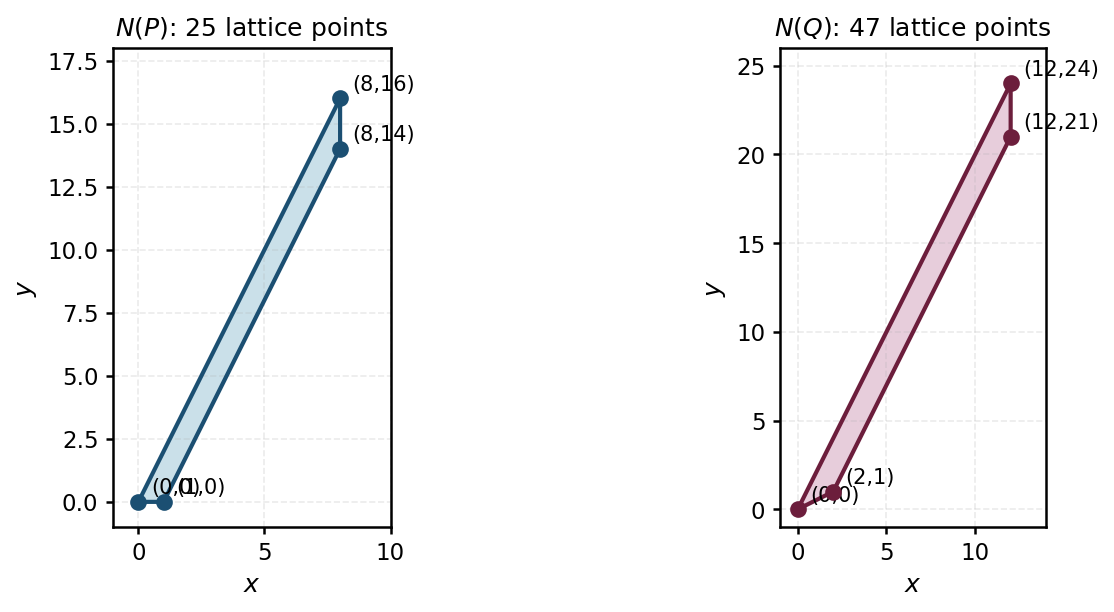
\includegraphics[width=0.95\linewidth]{figures_ab/fig1_newton_polygons.png}
\caption{The branch~(a,b) Newton polygons of~\cite[Proposition~4.3(2)]{GGHV}, checked against v1, lines~495 and 599--600 of the text extraction. $N(P)$ contains $25$ lattice points and $N(Q)$ contains $47$.}
\label{ab:fig:polygons}
\end{figure}

\begin{figure}[htbp]
\centering
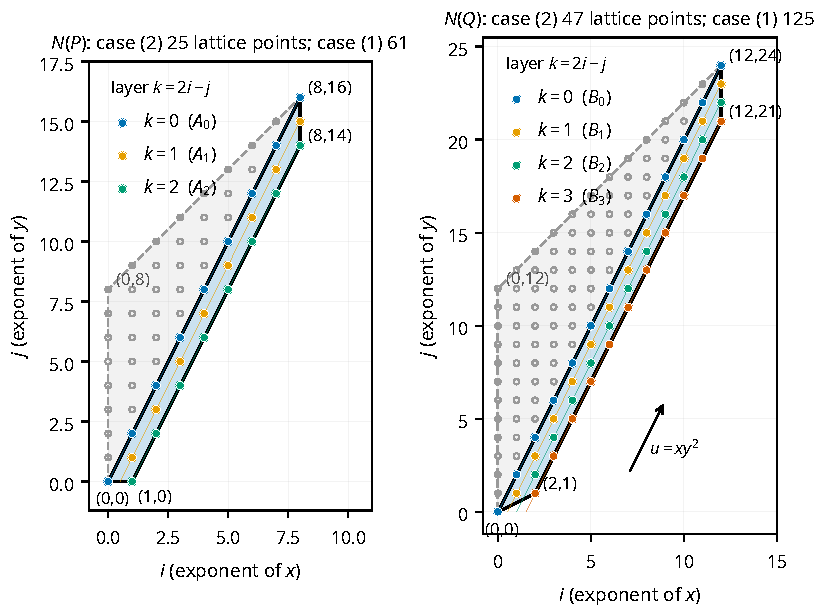
\includegraphics[width=\linewidth]{figures_jac/figJ1_newton_layers.pdf}
\caption{Case~(1) of GGHV Proposition~4.3 at the corner $(8,28)$ is case~(2) enlarged by one wedge at $i=0$. The panels show the lattice points of $N(P)$ (left) and $N(Q)$ (right) for the two normal forms, in the coordinates after $\varphi$ in which $[P,Q]=x^2$. Filled dots are case~(2): $N(P)=\mathrm{conv}\{(0,0),(1,0),(8,14),(8,16)\}$ with $25$ lattice points and $N(Q)=\mathrm{conv}\{(0,0),(2,1),(12,21),(12,24)\}$ with $47$. Each dot is coloured by its layer $k=2i-j$ in $P=\sum_k y^{-k}A_k(u)$, $Q=\sum_\ell y^{-\ell}B_\ell(u)$, $u=xy^2$; a layer is a line of slope $2$, the direction of $u$. Open grey dots and the dashed outline are the extra points of case~(1), with the added vertex $(0,8)$ ($61$ points) and $(0,12)$ ($125$ points). The points are generated from the half-plane predicates \texttt{inNP}, \texttt{inNQ}, \texttt{inNPc} and \texttt{inNQc} of the Lean sources, and their numbers agree with the lattice counts proved in the kernel. Case~(2) is excluded by \texttt{main\_theorem} (Theorem~\ref{ab:thm:main}) and case~(1) by \texttt{branch\_c\_eliminated}, both Lean kernel theorems on the standard axioms. Applying them to $(72,108)$ needs GGHV Proposition~4.3 to be exhaustive, which has not been verified, so the figure does not show $(72,108)$ excluded.}
\label{ab:fig:polygons-layers}
\end{figure}

\subsection{Main result}

Write $P=\sum a_{i,j}x^iy^j$ and $Q=\sum b_{i,j}x^iy^j$, and let $N_P$, $N_Q$ be the two polygons of~\eqref{ab:eq:polygons}.

\begin{theorem}[Elimination of the GGHV branch-(a,b) normal form]\label{ab:thm:main}
Let $K$ be a field of characteristic~$0$. Let $P,Q\in K[x,y]$ satisfy $\operatorname{supp}P\subset N_P$ and $\operatorname{supp}Q\subset N_Q$, suppose that $a_{1,0}\,a_{8,14}\,b_{2,1}\,b_{12,21}\neq0$, and suppose that $[P,Q]=\lambda x^2$ for some $\lambda\neq0$. Then $b_{12,24}=0$. In particular no pair $(P,Q)$ satisfies $\mathrm{NewtonNF2}(P,Q)$ (listing~\ref{ab:lst:def-newtonnf2}; the polygons are checked in~\S\ref{ab:sec:source}) together with $[P,Q]=\lambda x^2$.
\end{theorem}

\begin{corollary}[Lower-edge rigidity]\label{ab:cor:a816}
Under the hypotheses of Theorem~\ref{ab:thm:main}, also $a_{8,16}=0$. More precisely, every coefficient $a_{i,j}$ with $j\geq 2i-1$ and every coefficient $b_{i,j}$ with $j\geq 2i-2$ vanishes, except $a_{0,0}$ and $b_{0,0}$; that is, $P=P_2+a_{0,0}$ and $Q=Q_3+b_{0,0}$, where $P_2$ and $Q_3$ are the leading forms of~\S\ref{ab:sec:notation}.
\end{corollary}

In Lean this corollary is the theorem \texttt{lower\_\allowbreak{}edge\_\allowbreak{}rigidity} (listing~\ref{ab:lst:a816}), and the hypothesis $\lambda\neq0$ is not needed for it. A second proof of $a_{8,16}=0$, outside Lean, is an explicit ideal-membership certificate over $K_5$ (\filename{scripts/a816\_certificate/}), checked exactly by {\sc Singular} and by python-flint; see~\S\ref{ab:sec:lower-edge}. The corollary is not needed for the elimination, since $b_{12,24}=0$ already contradicts the required vertex $(12,24)$ of $N(Q)$.

\begin{remark}[Lean-to-mathematics correspondence]\label{ab:rem:nf2-bridge}
The Lean predicate \texttt{NewtonNF2} (listing~\ref{ab:lst:def-newtonnf2}) unfolds to
\[
\texttt{NewtonNF2}(P,Q)\iff
\begin{cases}
\operatorname{supp}P\subseteq N_P\ \text{and}\ \operatorname{supp}Q\subseteq N_Q
\ \text{(through \texttt{inNP}, \texttt{inNQ})},\\
a_{0,0},\,a_{1,0},\,a_{8,14},\,a_{8,16}\neq0,\\
b_{0,0},\,b_{2,1},\,b_{12,21},\,b_{12,24}\neq0 .
\end{cases}
\]
These are the support conditions of Theorem~\ref{ab:thm:main} together with the nonvanishing of the eight vertex coefficients. The predicates \texttt{inNP} and \texttt{inNQ} describe the polygons by half-planes; for $N_P$ these are $i\le 8$, $j\le 2i$ and $2i\le j+2$, and for $N_Q$ they are $i\le 12$, $j\le 2i$, $2i\le j+3$ and $i\le 2j$. They are tied to the vertex sets by \texttt{decide} checks on the duplicate predicates \texttt{latticeNP} and \texttt{latticeNQ}, which restate the same inequalities: the lattice-point counts ($25$ and $47$) and a vertex-membership check confirm that the eight vertices lie on the polygons. This is what lets the kernel-checked \texttt{main\_\allowbreak{}theorem} speak about the same $P,Q$ as Theorem~\ref{ab:thm:main}.
\end{remark}

\begin{corollary}[Conditional on GGHV]\label{ab:cor:gghv}
Assume \cite[Prop.~4.3]{GGHV}. Then no counterexample to the plane Jacobian conjecture arises in case~$(8,28)$, sub-cases~a) and~b).
\end{corollary}

The proof is computational but exact. We reduce the system of $72$ unknown coefficients to five triangular layers (Figure~\ref{ab:fig:layers}). We determine the top layer twice: by a Belyi-map argument resting on Riemann's existence theorem (Figure~\ref{ab:fig:top}), and by an algebraic argument formalized in Lean (\S\ref{ab:sec:chartproof}). We then show that no top-layer solution extends through the lower layers, using layer certificates that are also formalized in Lean (\S\ref{ab:sec:descent}). Key steps were checked in {\sc Singular}~4.4.1 and in Python with {\sc SymPy}; the scripts are archived with the paper.

\begin{figure}[htbp]
\centering
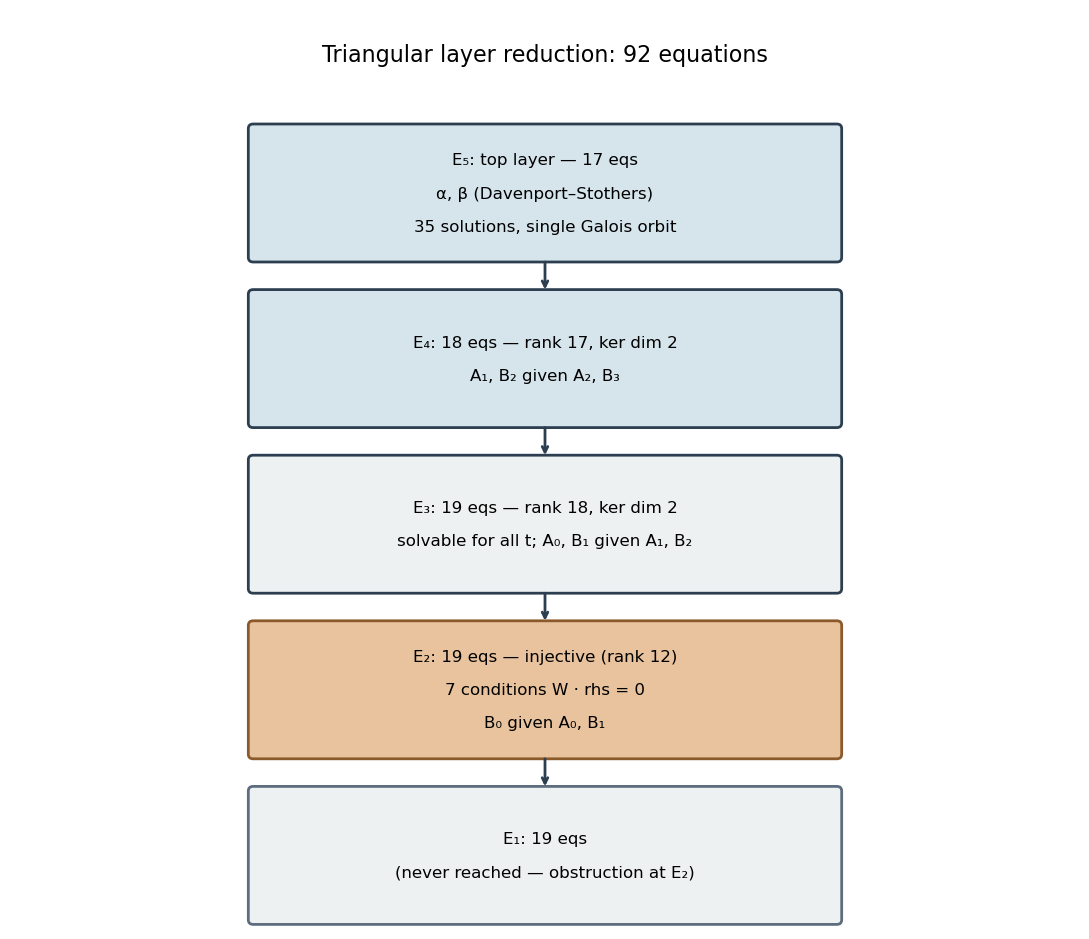
\includegraphics[width=0.75\linewidth]{figures_ab/fig2_layer_descent.png}
\caption{The triangular layer structure: $92$ equations in five layers. Each layer is affine-linear in its own unknowns once the layers above it are solved.}
\label{ab:fig:layers}
\end{figure}

\subsection{Logical status}

\begin{remark}\label{ab:rem:conditional}
Theorem~\ref{ab:thm:main} does not depend on GGHV. Its proof uses Proposition~\ref{ab:prop:top-class} for $m=7$, which we prove twice. On paper it follows from Riemann's existence theorem (\S\ref{ab:sec:top}). In \S\ref{ab:sec:chartproof} the classification it provides is proved algebraically in the normalized chart, and that proof is formalized in Lean as \texttt{chartClassification\_\allowbreak{}holds} (listing~\ref{ab:lst:proofchartclass}).

On the Lean side, \texttt{main\_\allowbreak{}theorem\_\allowbreak{}of\_\allowbreak{}chart} (listing~\ref{ab:lst:chart}) derives the NewtonNF2 form of Theorem~\ref{ab:thm:main} from the explicit statement \texttt{ChartClassification} (listing~\ref{ab:lst:def-chartclass}). The theorem \texttt{main\_\allowbreak{}theorem} (listing~\ref{ab:lst:unconditional}) combines it with \texttt{chartClassification\_\allowbreak{}holds} into one kernel-checked theorem that does not depend on GGHV Proposition~4.3, and \texttt{\#print axioms} reports for it only \texttt{propext}, \texttt{Classical.\allowbreak{}choice} and \texttt{Quot.\allowbreak{}sound}. The part $b_{12,24}=0$ follows from \texttt{no\_\allowbreak{}completion\_\allowbreak{}K5\_\allowbreak{}PQ} together with \texttt{topLayerClassification\_\allowbreak{}of\_\allowbreak{}chart} and \texttt{chartClassification\_\allowbreak{}holds}. The part $a_{8,16}=0$ of Corollary~\ref{ab:cor:a816} is \texttt{a816\_\allowbreak{}eq\_\allowbreak{}zero}, and the whole corollary is \texttt{lower\_\allowbreak{}edge\_\allowbreak{}rigidity} (listing~\ref{ab:lst:a816}). Both are kernel-checked on the same three axioms, and both reuse the descent down to $t=0$.

Outside Lean there is an explicit certificate $a_{8,16}^2=\sum_k H_k e_k$ over $K_5$. It is stored as the $76$ cofactors of $1=\sum_k z^2H_k e_k-(1+a_{8,16}z)(a_{8,16}z-1)$ in \filename{scripts/a816\_certificate/a816\_lift.txt}, checked exactly by {\sc Singular} and by python-flint, and it proves $a_{8,16}=0$ without the descent (\S\ref{ab:sec:lower-edge}). Only Corollary~\ref{ab:cor:gghv} also assumes GGHV Proposition~4.3.
\end{remark}

Grades are those of the author's evidence-grading scheme HLRE~v5.1, explained in Appendix~\ref{app:methods}; grades run from A (strongest) to D. The campaign record grades the elimination of branches~(a) and~(b), that is, the NewtonNF2 form of Theorem~\ref{ab:thm:main} as the kernel-checked theorem \texttt{main\_\allowbreak{}theorem}, at grade~A. The record gives no separate grade to the other statements of this part, and we assign none; instead we say for each statement whether it is kernel-checked, an exact machine computation, or a hand argument. The application to the Jacobian conjecture (Corollary~\ref{ab:cor:gghv}) is conditional on the correctness and exhaustiveness of~\cite[Prop.~4.3]{GGHV}, and nothing in this part excludes the degree pair $(72,108)$ unconditionally.

\subsection{Outline}

Section~\ref{ab:sec:notation} fixes notation and recalls the standard notions used later. Section~\ref{ab:sec:source} checks every base object against GGHV v1. Section~\ref{ab:sec:system} sets up the system of $72$ unknowns, and Section~\ref{ab:sec:layers} reduces it exactly to five layers. Section~\ref{ab:sec:normalization} fixes normalizations. Section~\ref{ab:sec:top} classifies the top layer, Section~\ref{ab:sec:descent} carries out the descent through the lower layers, and Section~\ref{ab:sec:obstruction} proves the final obstruction. Section~\ref{ab:sec:lifting} explains why the computations over $K_5$ hold in every field of characteristic zero. Section~\ref{ab:sec:conclusion} sums up; branch~(c) is eliminated in Part~II (Theorem~\ref{bc:thm:unconditional}). Section~\ref{ab:sec:attribution} covers prior work, attribution and independence.

The proof is organized around four certificates. Certificate~I, the Newton reduction, shows that $[P,Q]=\lambda x^2$ implies the layer identities $E_5,\dots,E_1$ (\S\ref{ab:sec:layers}). Certificate~II, top-layer completeness, shows that $E_5$ leaves exactly five torus orbits, all defined over $K_5$ (\S\ref{ab:sec:top} and~\S\ref{ab:sec:chartproof}). Certificate~III, the descent obstruction, shows that $E_4$, $E_3$ and $E_2$ force a compatibility ideal equal to $(t_1,t_2)^5$, hence $t=0$ (\S\ref{ab:sec:descent} and~\S\ref{ab:sec:obstruction}). Certificate~IV, vertex destruction, shows that $t=0$ forces $B_0'=0$ and hence $b_{12,24}=0$ (Corollary~\ref{ab:cor:t0}). The rigidity $a_{8,16}=0$ of Corollary~\ref{ab:cor:a816} is a supplement that Theorem~\ref{ab:thm:main} does not use. The logical chain is
\[
\boxed{\text{counterexample in case }(8,28)\xrightarrow{\ \text{GGHV 4.3}\ } \text{NewtonNF2},\ [P,Q]=\lambda x^2 \xrightarrow{\ \text{Thm.~\ref{ab:thm:main}}\ } \text{contradiction}}
\]
and only its first arrow uses GGHV. Table~\ref{ab:tab:dependence} lists the dependence of each step.

\begin{table}[htbp]
\centering
\begin{tabular}{lc}
\toprule
Result & Depends on GGHV? \\ \midrule
Layer reduction & no \\
Top-layer classification & no \\
$K_5$ descent & no \\
$b_{12,24}=0$ & no \\
$a_{8,16}=0$ & no \\
Theorem~\ref{ab:thm:main} & no \\
Corollary~\ref{ab:cor:gghv} (Jacobian application) & yes\\
\bottomrule
\end{tabular}
\caption{Dependence of the steps of Part~I on GGHV Proposition~4.3.}
\label{ab:tab:dependence}
\end{table}

\section{Setting and notation}\label{ab:sec:notation}

This section collects the definitions used in the rest of Part~I. Readers who know them can skip to~\S\ref{ab:sec:source}.

\subsection{Supports, Newton polygons and vertex coefficients}

For $P=\sum a_{i,j}x^iy^j\in K[x,y]$ the \emph{support} is $\operatorname{supp}P=\{(i,j)\in\mathbb{Z}_{\ge0}^2: a_{i,j}\neq0\}$, and the \emph{Newton polygon} $N(P)$ is the convex hull of $\operatorname{supp}P$ in $\mathbb{R}^2$. GGHV list a Newton polygon by its vertices. If $(i,j)$ is a vertex of $N(P)$, then $a_{i,j}\neq0$ automatically; we call $a_{i,j}$ a \emph{vertex coefficient}. Conversely, to say that a candidate pair has prescribed polygons $N_P,N_Q$ means two things: the supports lie in $N_P$ and $N_Q$, and the vertex coefficients do not vanish. This is exactly the predicate \texttt{NewtonNF2} of Remark~\ref{ab:rem:nf2-bridge}. We write \emph{GGHV normal form (2)} for the pair of polygons~\eqref{ab:eq:polygons}.

\subsection{The bracket}

The bracket $[P,Q]=P_xQ_y-P_yQ_x$ is $K$-bilinear and antisymmetric, and it is a derivation in each argument: $[PR,Q]=P[R,Q]+R[P,Q]$. The morphism $\varphi$ of GGHV ($\varphi(x)=x^{-1}$, $\varphi(y)=x^4y$) is not an automorphism, and it changes the bracket by the factor $-x^2$ (Proposition~\ref{ab:prop:gghv43}); this is why the target in~\eqref{ab:eq:polygons} is $[P,Q]=x^2$ rather than a constant. Since the two sides may be rescaled independently, we allow $[P,Q]=\lambda x^2$ with any $\lambda\neq0$.

\subsection{A grading and leading forms}

Give $x$ the weight $2$ and $y$ the weight $-1$, so that the monomial $x^iy^j$ has weight $2i-j$. A polynomial is \emph{weighted homogeneous of weight $k$} if all its monomials have weight $k$. Every $P$ splits uniquely as $P=\sum_kP_k$ with $P_k$ weighted homogeneous of weight $k$; the component of highest weight is the \emph{leading form}. The inequalities $j\le 2i\le j+2$ of $N_P$ say exactly that $0\le 2i-j\le 2$, so $P=P_0+P_1+P_2$ with leading form $P_2$. In the same way the inequalities $j\le 2i\le j+3$ of $N_Q$ give $Q=Q_0+Q_1+Q_2+Q_3$ with leading form $Q_3$.

The monomial $u:=xy^2$ has weight $0$, and $x^iy^j=u^i\,y^{j-2i}$. Hence a weighted homogeneous polynomial of weight $k$ can be written as $y^{-k}A(u)$ with $A\in K[u]$, the coefficient of $u^i$ in $A$ being $a_{i,2i-k}$. Differentiation by $x$ lowers the weight by $2$ and differentiation by $y$ raises it by $1$, so for weighted homogeneous $P,Q$ of weights $a,b$ the products $P_xQ_y$ and $P_yQ_x$ both have weight $(a-2)+(b+1)=a+b-1$. Thus $[P_a,Q_b]$ is weighted homogeneous of weight $a+b-1$. The polynomial $x^2$ has weight $4$, and $x^2=u^2y^{-4}$.

For $a,b\in\mathbb{Z}_{\ge0}$ and $A,B\in K[u]$ we put
\[
\mathrm{LT}_{a,b}(A,B):=a\,A\,B'-b\,A'\,B,
\]
where $'$ is $d/du$. In Lean this operator is \texttt{layerTerm} (listing~\ref{ab:lst:def-layerterm}).

\subsection{Belyi maps, passports and the Davenport--Stothers equation}

A \emph{Belyi map} is a nonconstant rational function $\phi\colon\mathbb{P}^1\to\mathbb{P}^1$ whose critical values lie in a set of three points. If $\phi$ has degree $n$, then over each of the three branch points the ramification indices form a partition of $n$; the triple of partitions is the \emph{passport} of $\phi$. We write a partition multiplicatively, so $[2^{10}1]$ means ten points of index $2$ and one unramified point. Riemann's existence theorem says that, up to isomorphism of covers, degree-$n$ covers of $\mathbb{P}^1$ branched over three given points correspond to simultaneous $S_n$-conjugacy classes of triples $(g_0,g_1,g_\infty)$ of permutations that generate a transitive subgroup and satisfy $g_0g_1g_\infty=1$, the cycle type of each $g$ being the partition over the corresponding point.

For polynomials $f,g\in\mathbb{C}[s]$ with $f^3\neq g^2$, Davenport's theorem~\cite{Davenport} states that $\deg(f^3-g^2)\ge\tfrac12\deg f+1$, and Stothers~\cite{Stothers} proved that the bound is attained for every even $\deg f$. We call the equation $2fg'-3f'g=c$ with $c\in\mathbb{C}^\times$ the \emph{Davenport--Stothers equation}; in~\S\ref{ab:sec:top} we show that its solutions are extremal for Davenport's bound.

\subsection{The field \texorpdfstring{$K_5$}{K5} and the torus}

Put $R(w)=w^5-w^4+3w^3+3w^2+26$ and $K_5=\mathbb{Q}[w]/(R)$. We show in Lemma~\ref{ab:lem:basechange} that $R$ is irreducible, so $K_5$ is a number field of degree~$5$. All exact descent computations are done over $K_5$.

The equations below have a group of scaling symmetries, which we call \emph{the torus}: for $\rho,\sigma,\varepsilon\in K^\times$ the substitution $A(u)\mapsto\rho\,\varepsilon^{-1}A(\varepsilon u)$ on the $P$-side and $B(u)\mapsto\sigma\,\varepsilon^{-2}B(\varepsilon u)$ on the $Q$-side multiplies the coefficient of $u^i$ by $\rho\varepsilon^{i-1}$, respectively $\sigma\varepsilon^{k-2}$ for $u^k$ (this is the form used in \texttt{TopLayerClassification}, listing~\ref{ab:lst:def-toplayerclass}). Two solutions related in this way are said to lie in the same \emph{torus orbit}.

\subsection{Coefficient matrices and ideals}

When a polynomial identity in $u$ is linear in a vector $x$ of unknown coefficients, comparing the coefficients of $1,u,u^2,\dots$ gives a linear system $Mx=K$; we call $M$ the \emph{coefficient matrix} of the layer. A row vector $v$ with $v^{\mathrm T}M=0$ is a \emph{left null vector}, and $Mx=K$ is solvable only if $v^{\mathrm T}K=0$ for every such $v$; these are the \emph{compatibility conditions}. For an ideal $I$ and a polynomial $f$, the saturation is $I:f^\infty=\{g:f^Ng\in I\text{ for some }N\}$. Ideal membership $g\in I$ is certified by explicit cofactors $c_i$ with $g=\sum_ic_ie_i$ for generators $e_i$ of $I$; such a certificate can be checked by expansion alone. The Rabinowitsch form of a certificate that $g$ vanishes on $V(I)$ writes $1$ as a combination of the $e_i$ and of $1-zg$ for a new variable $z$.

\subsection{Lean, the kernel and \texttt{\#print axioms}}

Lean~4 is an interactive theorem prover. Every proof it accepts is reduced to a term of its type theory, and a small trusted program, the \emph{kernel}, re-checks that term. The command \texttt{\#print axioms T} lists every axiom on which the theorem \texttt{T} depends, through all the lemmas it uses. A theorem whose list contains only \texttt{propext}, \texttt{Classical.\allowbreak{}choice} and \texttt{Quot.\allowbreak{}sound}, the three standard axioms of Lean's foundations used throughout Mathlib, has been checked by the kernel with no gaps: an unfinished proof (\texttt{sorry}) would appear as the axiom \texttt{sorryAx}, and the compiled-code shortcut \texttt{native\_\allowbreak{}decide} would appear as an extra axiom. We say such a theorem is \emph{kernel-checked}. The kernel checks that the proofs prove the stated propositions; whether a stated proposition says what the mathematics says is checked by a human reader, which is why we print the relevant Lean definitions verbatim. The Lean listings in this part are extracted mechanically from the source files, with the file name and a hash prefix in each caption.

\section{Source data}\label{ab:sec:source}

We checked every base object directly against version~1 of~\cite{GGHV} (arXiv:2204.14178v1), downloaded from \url{https://arxiv.org/pdf/2204.14178v1} and converted with \texttt{pdftotext -layout}. No proof was drafted until the polygons, the bracket and $\varphi$ had been confirmed character by character against the text of GGHV. The result we use is the following; $L^{(1)}$ is GGHV's ring of polynomials in $y$ with Laurent coefficients in $x$, in which their reduction takes place.

\begin{proposition}[{\cite[Proposition~4.3]{GGHV}, checked against the source}]\label{ab:prop:gghv43}
If there is a counterexample to the Jacobian conjecture in case~$(8,28)$, then there exist $P,Q\in L^{(1)}$ with $[P,Q]=x^2$ and one of the following holds:
\begin{enumerate}[nosep]
\item[(1)] $N(P)=\{(0,0),(1,0),(8,14),(8,16),(0,8)\}$ and\\ $N(Q)=\{(0,0),(2,1),(12,21),(12,24),(0,12)\}$;
\item[(2)] $N(P)=\{(0,0),(1,0),(8,14),(8,16)\}$ and $N(Q)=\{(0,0),(2,1),(12,21),(12,24)\}$.
\end{enumerate}
\end{proposition}

\begin{proof}[Source locations]
In the \texttt{pdftotext -layout} extraction of v1, line~33 fixes the bracket convention $[P,Q]:=P_xQ_y-P_yQ_x\in K^\times$. Line~492 opens ``Proposition~4.3 (Case $(8,28)$)'', and line~493 continues ``with $[P,Q]=x^2$'' (the exponent appears as \texttt{x2} in the extraction). Line~495 gives the case~(2) polygons, as displayed above. Lines~596--597 introduce the morphism $\varphi(x)=x^{-1}$, $\varphi(y)=x^4y$, note that it is not an automorphism, and record the chain rule $[\varphi(P),\varphi(Q)]=-[P,Q]x^2$. Lines~599--600 state that in the cases a) and b) the Newton polygons become exactly the case~(2) polygons. A verification script, \filename{source\_gate\_verify.py}, asserts each of these lines automatically and exits with a nonzero status if any check fails.
\end{proof}

From now on we work only with case~(2), branches~(a) and~(b).

\section{The polynomial system}\label{ab:sec:system}

\subsection{Lattice points}

The polygons~\eqref{ab:eq:polygons} are cut out by the half-planes of Remark~\ref{ab:rem:nf2-bridge}. Direct enumeration gives
\begin{equation}
|N(P)\cap\mathbb{Z}^2|=25,\qquad |N(Q)\cap\mathbb{Z}^2|=47 .
\end{equation}
We cross-check with Pick's theorem, which says that a lattice polygon of area $\mathcal{A}$ with $b$ lattice points on its boundary has $i=\mathcal{A}-b/2+1$ interior lattice points. For $N(P)$ the shoelace formula on the vertices $(0,0),(1,0),(8,14),(8,16)$ gives $\mathcal{A}=15$, and the four edges carry $\gcd(1,0)+\gcd(7,14)+\gcd(0,2)+\gcd(8,16)=1+7+2+8=18$ boundary points. Hence $i=15-9+1=7$ and the total is $7+18=25$. For $N(Q)$ the same computation gives $\mathcal{A}=33$, $b=26$, $i=33-13+1=21$, and the total is $21+26=47$. So $P$ and $Q$ have together $25+47=72$ unknown coefficients. The two constant terms do not enter $[P,Q]$, which leaves $70$ effective unknowns, but we keep all $72$ for the layer structure.

\subsection{Layer supports}

We now sort the lattice points by weight. A point $(i,j)$ of $N(P)$ has weight $k=2i-j\in\{0,1,2\}$, so
\begin{equation}\label{ab:eq:decomp}
P=A_0(u)+y^{-1}A_1(u)+y^{-2}A_2(u),\qquad Q=B_0(u)+y^{-1}B_1(u)+y^{-2}B_2(u)+y^{-3}B_3(u),
\end{equation}
where $u=xy^2$ and the coefficient of $u^i$ in $A_k$ is $a_{i,2i-k}$, and in $B_k$ it is $b_{i,2i-k}$. The ranges of $i$ follow from the half-planes. For $A_0$ ($j=2i$) the condition $i\le8$ gives $0\le i\le 8$. For $A_1$ and $A_2$ the condition $j=2i-k\ge0$ adds $i\ge1$, so $1\le i\le8$. For $B_0$ we get $0\le i\le12$. For $B_1$, $j=2i-1\ge0$ forces $i\ge1$. For $B_2$, the condition $i\le 2j=4i-4$ forces $i\ge 2$, and for $B_3$, $i\le 4i-6$ again forces $i\ge2$. Altogether
\[
\begin{array}{lll}
A_0\colon u^0,\dots,u^8, & A_1\colon u^1,\dots,u^8, & A_2\colon u^1,\dots,u^8,\\
B_0\colon u^0,\dots,u^{12}, & B_1\colon u^1,\dots,u^{12}, & B_2,\,B_3\colon u^2,\dots,u^{12},
\end{array}
\]
which accounts for $9+8+8=25$ and $13+12+11+11=47$ coefficients. In this notation the eight vertex coefficients are $a_{1,0}$ and $a_{8,14}$ (the coefficients of $u$ and $u^8$ in $A_2$), $a_{8,16}$ (of $u^8$ in $A_0$), $a_{0,0}$, then $b_{2,1}$ and $b_{12,21}$ (of $u^2$ and $u^{12}$ in $B_3$), $b_{12,24}$ (of $u^{12}$ in $B_0$) and $b_{0,0}$. These are the supports used in \texttt{no\_\allowbreak{}completion\_\allowbreak{}K5} (listing~\ref{ab:lst:main}).

Writing $[P,Q]=\lambda x^2$ out in the coefficients gives a system of bilinear equations in the $72$ unknowns. Solving it directly is impractical, and we use instead the exact layer reduction of the next section. Direct expansion remains feasible for checking that reduction, as in Proposition~\ref{ab:prop:layers}.

\section{Exact layer reduction}\label{ab:sec:layers}

The grading of~\S\ref{ab:sec:notation} splits the single equation $[P,Q]=\lambda x^2$ into its weighted homogeneous components. The first step is to compute the bracket of two layer terms.

\begin{lemma}[Bracket of layer terms]\label{ab:lem:layerbracket}
For $a,b\in\mathbb{Z}_{\ge0}$ and $A,B\in K[u]$, with $u=xy^2$,
\[
\bigl[y^{-a}A(u),\,y^{-b}B(u)\bigr]=y^{1-a-b}\,\mathrm{LT}_{a,b}(A,B)(u).
\]
\end{lemma}

\begin{proof}
Since $\partial u/\partial x=y^2$ and $\partial u/\partial y=2xy$, the chain rule gives
\[
\partial_x\bigl(y^{-a}A\bigr)=y^{2-a}A',\qquad \partial_y\bigl(y^{-a}A\bigr)=-a\,y^{-a-1}A+2x\,y^{1-a}A',
\]
and likewise for $y^{-b}B$. Substituting into $P_xQ_y-P_yQ_x$,
\begin{align*}
\bigl[y^{-a}A,\,y^{-b}B\bigr]
&=y^{2-a}A'\bigl(-b\,y^{-b-1}B+2x\,y^{1-b}B'\bigr)-\bigl(-a\,y^{-a-1}A+2x\,y^{1-a}A'\bigr)\,y^{2-b}B'\\
&=-b\,y^{1-a-b}A'B+2x\,y^{3-a-b}A'B'+a\,y^{1-a-b}AB'-2x\,y^{3-a-b}A'B'.
\end{align*}
The two terms containing $2x\,y^{3-a-b}A'B'$ cancel, and what remains is $y^{1-a-b}(aAB'-bA'B)$.
\end{proof}

Insert~\eqref{ab:eq:decomp} into $[P,Q]$ and expand by bilinearity. By Lemma~\ref{ab:lem:layerbracket} the term $[y^{-a}A_a,y^{-b}B_b]$ contributes $y^{1-a-b}\mathrm{LT}_{a,b}(A_a,B_b)$, and the right-hand side is $\lambda x^2=\lambda u^2y^{-4}$. Comparing the coefficients of each power $y^{1-n}$, that is, comparing weighted homogeneous components of weight $n-1$, gives one identity in $K[u]$ for each value of $n=a+b$:
\begin{align*}
E_5&\colon\ \mathrm{LT}_{2,3}(A_2,B_3)=\lambda u^2,\\
E_4&\colon\ \mathrm{LT}_{2,2}(A_2,B_2)+\mathrm{LT}_{1,3}(A_1,B_3)=0,\\
E_3&\colon\ \mathrm{LT}_{2,1}(A_2,B_1)+\mathrm{LT}_{1,2}(A_1,B_2)+\mathrm{LT}_{0,3}(A_0,B_3)=0,\\
E_2&\colon\ \mathrm{LT}_{2,0}(A_2,B_0)+\mathrm{LT}_{1,1}(A_1,B_1)+\mathrm{LT}_{0,2}(A_0,B_2)=0,\\
E_1&\colon\ \mathrm{LT}_{1,0}(A_1,B_0)+\mathrm{LT}_{0,1}(A_0,B_1)=0 .
\end{align*}
For $n=0$ the only term is $\mathrm{LT}_{0,0}(A_0,B_0)=0$, which vanishes identically, so the five identities are in fact equivalent to $[P,Q]=\lambda x^2$; only the implication is needed below. Unfolding $\mathrm{LT}$, the three layers we use most often read
\begin{align*}
E_4&\colon\ 2\bigl(A_2B_2'-A_2'B_2\bigr)+\bigl(A_1B_3'-3A_1'B_3\bigr)=0,\\
E_2&\colon\ 2A_2B_0'+\bigl(A_1B_1'-A_1'B_1\bigr)-2A_0'B_2=0,\\
E_1&\colon\ A_1B_0'-A_0'B_1=0 .
\end{align*}

Each identity $E_n$ is a polynomial identity in $u$, and an \emph{equation} of the layer is the coefficient of one power of $u$. With the supports of~\S\ref{ab:sec:system}, the left side of $E_5$ has terms in $u^2,\dots,u^{18}$ (the coefficient of $u^{19}$ is $(2\cdot12-3\cdot8)\,a_{8,14}b_{12,21}=0$), giving $17$ equations; $E_4$ has terms in $u^2,\dots,u^{19}$, giving $18$; and $E_3$, $E_2$, $E_1$ have terms in $u^1,\dots,u^{19}$, giving $19$ each.

\begin{proposition}[Exact layer reduction]\label{ab:prop:layers}
The system $[P,Q]=\lambda x^2$ on the $72$ coefficients implies the five one-variable polynomial identities $E_1,\dots,E_5$, which consist of the following numbers of scalar equations:
\begin{center}
\begin{tabular}{ccl}
\toprule
Layer & Equations & Unknowns (given the layers above) \\
\midrule
$E_5$ & $17$ & top: $\alpha,\beta$ \\
$E_4$ & $18$ & $A_1,B_2$ given $A_2,B_3$ \\
$E_3$ & $19$ & $A_0,B_1$ given $A_1,B_2$ \\
$E_2$ & $19$ & $B_0$ given $A_0,B_1$ \\
$E_1$ & $19$ & none new; a consistency layer \\
\midrule
Total & $92$ & \\
\bottomrule
\end{tabular}
\end{center}
The reduction was also verified as a polynomial identity (script \filename{C1\_layer\_reduction.sing}) with all $72$ coefficients treated as indeterminates; the residual is identically zero.
\end{proposition}

\begin{proof}
The derivation above proves the implication. As an independent check, the script \filename{C1\_layer\_reduction.sing} ({\sc Singular}) substitutes~\eqref{ab:eq:decomp} into $[P,Q]-x^2$, collects by powers of $y$, expands each $E_i$ in the $72$ indeterminates, and compares with the direct bilinear expansion of $[P,Q]-x^2$; the difference is zero as a polynomial in $72$ variables. In Lean the reduction is the kernel-checked theorem \texttt{layers\_\allowbreak{}of\_\allowbreak{}jac} (listing~\ref{ab:lst:layers}).
\end{proof}

% BEGIN-MECHANICAL:lst:layers
\begin{leanlisting}{Mechanically extracted from \texttt{Jacobian/BranchAbLayers.lean} (sha256 \texttt{7c16141b4b126b3e}); statement verbatim, proof elided.}{ab:lst:layers}
theorem layers_of_jac (lam : K) (A₀ A₁ A₂ B₀ B₁ B₂ B₃ : Polynomial K)
    (p₀ p₁ p₂ q₀ q₁ q₂ q₃ : MvPolynomial (Fin 2) K)
    (hp₀ : X 1 ^ 0 * p₀ = evH A₀) (hp₁ : X 1 ^ 1 * p₁ = evH A₁) (hp₂ : X 1 ^ 2 * p₂ = evH A₂)
    (hq₀ : X 1 ^ 0 * q₀ = evH B₀) (hq₁ : X 1 ^ 1 * q₁ = evH B₁) (hq₂ : X 1 ^ 2 * q₂ = evH B₂)
    (hq₃ : X 1 ^ 3 * q₃ = evH B₃)
    (hJ : jac (p₀ + p₁ + p₂) (q₀ + q₁ + q₂ + q₃) = C lam * X 0 ^ 2) :
    layerTerm 2 3 A₂ B₃ = Polynomial.C lam * Polynomial.X ^ 2 /\
    layerTerm 2 2 A₂ B₂ + layerTerm 1 3 A₁ B₃ = 0 /\
    layerTerm 2 1 A₂ B₁ + layerTerm 1 2 A₁ B₂ + layerTerm 0 3 A₀ B₃ = 0 /\
    layerTerm 2 0 A₂ B₀ + layerTerm 1 1 A₁ B₁ + layerTerm 0 2 A₀ B₂ = 0 /\
    layerTerm 1 0 A₁ B₀ + layerTerm 0 1 A₀ B₁ = 0 := by
  -- proof body elided (see artifact)
\end{leanlisting}
% END-MECHANICAL:lst:layers

The basic definitions used in that statement are printed in full, since only a human reader, not the Lean kernel, can check that a definition means what it is meant to mean.
% BEGIN-MECHANICAL:lst:def-jac
\begin{leanlisting}{Mechanically extracted from \texttt{Jacobian/BranchAbLayers.lean} (sha256 \texttt{7c16141b4b126b3e}); definition printed verbatim in full.}{ab:lst:def-jac}
def jac (P Q : MvPolynomial (Fin 2) K) : MvPolynomial (Fin 2) K :=
  pderiv 0 P * pderiv 1 Q - pderiv 1 P * pderiv 0 Q
\end{leanlisting}
% END-MECHANICAL:lst:def-jac
% BEGIN-MECHANICAL:lst:def-uu
\begin{leanlisting}{Mechanically extracted from \texttt{Jacobian/BranchAbLayers.lean} (sha256 \texttt{7c16141b4b126b3e}); definition printed verbatim in full.}{ab:lst:def-uu}
def uu : MvPolynomial (Fin 2) K := X 0 * X 1 ^ 2
\end{leanlisting}
% END-MECHANICAL:lst:def-uu
% BEGIN-MECHANICAL:lst:def-evh
\begin{leanlisting}{Mechanically extracted from \texttt{Jacobian/BranchAbLayers.lean} (sha256 \texttt{7c16141b4b126b3e}); definition printed verbatim in full.}{ab:lst:def-evh}
def evH : Polynomial K →ₐ[K] MvPolynomial (Fin 2) K := Polynomial.aeval (uu (K := K))
\end{leanlisting}
% END-MECHANICAL:lst:def-evh
% BEGIN-MECHANICAL:lst:def-layerterm
\begin{leanlisting}{Mechanically extracted from \texttt{Jacobian/BranchAbLayers.lean} (sha256 \texttt{7c16141b4b126b3e}); definition printed verbatim in full.}{ab:lst:def-layerterm}
def layerTerm (a b : Nat) (A B : Polynomial K) : Polynomial K :=
  (a : Polynomial K) * A * Polynomial.derivative B - (b : Polynomial K) * Polynomial.derivative A * B
\end{leanlisting}
% END-MECHANICAL:lst:def-layerterm

In Lean the hypothesis $y^k p_k=\mathrm{evH}(A_k)$ says that $p_k=y^{-k}A_k(xy^2)$, matching~\eqref{ab:eq:decomp}. The system is triangular (Figure~\ref{ab:fig:layers}): $E_5$ involves only the top-layer unknowns, and each $E_i$ with $i<5$ is affine-linear in its own unknowns once a solution of the layers above is fixed. This is the structural fact that makes the problem tractable, and it is not a computational accident. The $E_i$ are the weighted homogeneous components of $[P,Q]=\lambda x^2$ for the grading $w(x)=2$, $w(y)=-1$ induced by the polygons, and $\mathrm{LT}_{a,b}$ is the bracket of two homogeneous components written in the variable $u$.

\section{Normalization}\label{ab:sec:normalization}

The torus of~\S\ref{ab:sec:notation} acts on the top-layer unknowns, and we use it to fix two coefficients. Since $a_{1,0}$ and $a_{8,14}$ are the coefficients of $u$ and $u^8$ in $A_2$, the torus multiplies them by $\rho$ and $\rho\varepsilon^7$. Choosing $\rho$ and then $\varepsilon^7$ we may assume, without loss of generality,
\begin{equation}\label{ab:eq:normalization}
a_{1,0}=a_{8,14}=1,
\end{equation}
and we leave $a_{8,16}$ free. This fixes $\rho$ and $\varepsilon^7$ but not $\varepsilon$ itself: the remaining one-dimensional torus acts through the $y$-weight grading of the layer decomposition (\S\ref{ab:sec:layers}), and its finite subgroup $\mu_7$ of seventh roots of unity gives $7$ chart points in each torus orbit.

\begin{remark}[Lean chart normalization]
The Lean formalization uses chart coordinates $(a_1,\dots,a_7,b_0,\dots,b_9)$ for $\alpha=A_2/u=1+a_1u+\dots+a_7u^7$ and $\beta=B_3/u^2=b_0+b_1u+\dots+b_9u^9+u^{10}$, with the torus normalization $a_7^3 b_0^2 = 1$ (see \texttt{ChartClassification} in \filename{Jacobian/BranchAbChart.lean}). Once $\alpha_0=1$ and $\beta_{10}=1$ are fixed, the remaining scaling $u\mapsto\kappa u$, followed by the rescaling that restores $\beta_{10}=1$, multiplies $a_i$ by $\kappa^i$ and $b_k$ by $\kappa^{k-10}$. So it acts on $a_7$ with weight~$7$, on $b_0$ with weight~$-10$, and on $a_7^3 b_0^2$ with weight $3\cdot7+2\cdot(-10)=1$. The condition $a_7^3 b_0^2 = 1$ therefore fixes $\kappa$ completely, with no seventh-root ambiguity: the Lean chart meets each torus orbit exactly once, giving $5$ points rather than $35$. The chart~\eqref{ab:eq:normalization} meets each orbit $7$ times. The two charts are related by a torus element that requires a seventh root.
\end{remark}

\subsection{Vertex conditions used}\label{ab:sec:lower-edge}

The proof uses the vertices $(1,0)$ and $(2,1)$, equivalently $\lambda\neq0$; the vertex $(8,14)$, for the normalization and the degree of the top layer; and $(12,24)$, for the exclusion of $t=0$ in~\S\ref{ab:sec:t0}. The vertex $(8,16)$ is left free in \texttt{main\_\allowbreak{}theorem}. Once $E_1$ is included, $a_{8,16}=0$ is forced (Corollary~\ref{ab:cor:a816}). This gives a second contradiction, from the lower edge: \texttt{main\_\allowbreak{}theorem\_\allowbreak{}lower\_\allowbreak{}edge} (listing~\ref{ab:lst:a816-nf2}) refutes $\mathrm{NewtonNF2}$ without using the vertex $(12,24)$. It shares the descent down to $t=0$ with \texttt{main\_\allowbreak{}theorem}. The explicit certificate over $K_5$ (\filename{scripts/a816\_certificate/}, checked exactly by {\sc Singular} and by python-flint) reaches $a_{8,16}=0$ outside Lean and without the descent.

The torus acts compatibly on all layers. The Lean theorem \texttt{layers\_\allowbreak{}transport} (listing~\ref{ab:lst:torus}) states that if $E_4$, $E_3$, $E_2$ hold, they still hold after the substitution $A\mapsto\alpha\cdot\mathrm{sc}_\kappa A$, $B\mapsto\beta\cdot\mathrm{sc}_\kappa B$ applied to every layer, where $\mathrm{sc}_\kappa$ rescales $u$ by $\kappa$.

% BEGIN-MECHANICAL:lst:torus
\begin{leanlisting}{Mechanically extracted from \texttt{Jacobian/BranchAbTorus.lean} (sha256 \texttt{97918673d5c4dc09}); statement verbatim, proof elided.}{ab:lst:torus}
theorem layers_transport (α β κ : K) (A₀ A₁ A₂ B₀ B₁ B₂ B₃ : K[X])
    (E4 : layerTerm 2 2 A₂ B₂ + layerTerm 1 3 A₁ B₃ = 0)
    (E3 : layerTerm 2 1 A₂ B₁ + layerTerm 1 2 A₁ B₂ + layerTerm 0 3 A₀ B₃ = 0)
    (E2 : layerTerm 2 0 A₂ B₀ + layerTerm 1 1 A₁ B₁ + layerTerm 0 2 A₀ B₂ = 0) :
    layerTerm 2 2 (C α * sc κ A₂) (C β * sc κ B₂) + layerTerm 1 3 (C α * sc κ A₁) (C β * sc κ B₃) = 0 /\
    layerTerm 2 1 (C α * sc κ A₂) (C β * sc κ B₁) + layerTerm 1 2 (C α * sc κ A₁) (C β * sc κ B₂) +
      layerTerm 0 3 (C α * sc κ A₀) (C β * sc κ B₃) = 0 /\
    layerTerm 2 0 (C α * sc κ A₂) (C β * sc κ B₀) + layerTerm 1 1 (C α * sc κ A₁) (C β * sc κ B₁) +
      layerTerm 0 2 (C α * sc κ A₀) (C β * sc κ B₂) = 0 := by
  -- proof body elided (see artifact)
\end{leanlisting}
% END-MECHANICAL:lst:torus

\section{The top layer}\label{ab:sec:top}

\subsection{The Davenport--Stothers equation}

The top layer $E_5$ involves only $A_2$ and $B_3$, whose supports start at $u$ and $u^2$. We therefore write $A_2=u\alpha$ and $B_3=u^2\beta$. The vertices $(8,14)\in N(P)$ and $(12,21)\in N(Q)$ force $\deg\alpha=8-1=7$ and $\deg\beta=12-2=10$, and the vertices $(1,0)$ and $(2,1)$ force $\alpha(0)\ne0$ and $\beta(0)\ne0$. We now rewrite $E_5$ in terms of $\alpha$ and $\beta$. By definition of $\mathrm{LT}_{2,3}$,
\begin{align*}
\mathrm{LT}_{2,3}(u\alpha,u^2\beta)
&=2\,u\alpha\,(u^2\beta)'-3\,(u\alpha)'\,u^2\beta\\
&=2u\alpha\,(2u\beta+u^2\beta')-3(\alpha+u\alpha')\,u^2\beta\\
&=4u^2\alpha\beta+2u^3\alpha\beta'-3u^2\alpha\beta-3u^3\alpha'\beta\\
&=u^2\bigl(\alpha\beta+u\,(2\alpha\beta'-3\alpha'\beta)\bigr).
\end{align*}
Dividing $E_5$ by $u^2$, and rescaling so that $\lambda=1$, we obtain
\begin{equation}\label{ab:eq:e5}
\alpha\beta+u\,(2\alpha\beta'-3\alpha'\beta)=1 .
\end{equation}
Comparing coefficients, the coefficient of $u^n$ on the left is $\sum_{i+k=n}(1+2k-3i)\,\alpha_i\beta_k$. For $n=17=\deg\alpha+\deg\beta$ the factor is $1+2\cdot10-3\cdot7=0$, so the top coefficient vanishes identically. In general, with $m=\deg\alpha$ and $n=\deg\beta$, the top coefficient is $(1+2n-3m)\alpha_m\beta_n$, and~\eqref{ab:eq:e5} can hold with $m\ge1$ only if
\begin{equation}\label{ab:eq:mn}
1+2n-3m=0,
\end{equation}
which forces $m$ odd and $n=(3m-1)/2$.

Next we pass to the classical form. Put $u=s^2$, $f(s)=\alpha(s^2)$ and $g(s)=s\,\beta(s^2)$; then $f$ is even and $g$ is odd. By the chain rule $f'(s)=2s\,\alpha'(s^2)$ and $g'(s)=\beta(s^2)+2s^2\beta'(s^2)$. Hence
\begin{align*}
2fg'-3f'g&=2\alpha\bigl(\beta+2u\beta'\bigr)-3\cdot2s\alpha'\cdot s\beta\\
&=2\alpha\beta+4u\alpha\beta'-6u\alpha'\beta\\
&=2\bigl(\alpha\beta+u(2\alpha\beta'-3\alpha'\beta)\bigr),
\end{align*}
all evaluated at $u=s^2$. So~\eqref{ab:eq:e5} becomes the Davenport--Stothers equation~\cite{Stothers,Davenport}
\begin{equation}
2fg'-3f'g=c,\qquad c=2\neq0,
\end{equation}
with $f$ even, $g$ odd, $\deg f=2m=14$ and $\deg g=2n+1=21$. These solutions are extremal for Davenport's bound. To see this, differentiate the quotient $g^2/f^3$:
\[
\frac{d}{ds}\frac{g^2}{f^3}=\frac{2gg'f-3g^2f'}{f^4}=\frac{g\,(2fg'-3f'g)}{f^4}=\frac{c\,g}{f^4}.
\]
The right side has order $\deg g-4\deg f=21-56=-35$ at $s=\infty$. Let $\kappa_\infty$ be the value of $g^2/f^3$ at $s=\infty$, the ratio of the leading coefficients. Then $g^2/f^3-\kappa_\infty$ has order $-34$ at $\infty$, so
\[
\deg\bigl(g^2-\kappa_\infty f^3\bigr)=3\deg f-34=42-34=8=k+1\qquad(k=7),
\]
which is exactly Davenport's lower bound $\tfrac12\deg f+1=8$: the pair is extremal. The cases $m=1,3,5,7$ all admit solutions, and $m=7$ is the case relevant to~\eqref{ab:eq:polygons}. The classification of the parity-constrained solutions ($f$ even, $g$ odd) is computed here by elimination; we do not claim that it follows from the literature.

\subsection{Classification}

\begin{proposition}[Top-layer solutions]\label{ab:prop:top-class}
In the normalization $\alpha_0=\beta_0=\alpha_m=1$, the system~\eqref{ab:eq:e5} with $\deg\alpha=m$ and $\deg\beta=(3m-1)/2$ has
\begin{enumerate}[nosep]
\item[(i)] for $m=3$: $3$ complex solutions, with eliminant $3a_2^3-32$, irreducible over $\mathbb{Q}$;
\item[(ii)] for $m=5$: $10$ complex solutions, with eliminant $9a_4^{10}+37200a_4^5+95051008$, irreducible over $\mathbb{Q}$;
\item[(iii)] for $m=7$: $35$ complex solutions in the chart~\eqref{ab:eq:normalization}, with eliminant $\mathcal{W}(a_6)$ of degree $35$.
\end{enumerate}
The case $m=7$ is the one relevant to~\eqref{ab:eq:polygons}.
\end{proposition}

\begin{proof}
We work over~$\mathbb{C}$. The Belyi classification below is topological and hence valid over~$\mathbb{C}$; the resulting count transfers to every field of characteristic~$0$ by base change, because the equations are defined over~$\mathbb{Q}$. We prove the upper bounds by the Belyi-map classification and then show that they are attained.

\emph{The Belyi map.} Let $(\alpha,\beta)$ solve~\eqref{ab:eq:e5}, write $E$ for its left side, and put $\phi=u\beta^2/\alpha^3$. By the quotient rule,
\[
\phi'=\frac{\beta^2}{\alpha^3}+\frac{2u\beta\beta'}{\alpha^3}-\frac{3u\beta^2\alpha'}{\alpha^4}
=\frac{\beta\,\bigl(\alpha\beta+2u\alpha\beta'-3u\alpha'\beta\bigr)}{\alpha^4}=\frac{\beta\,E}{\alpha^4}=\frac{\beta}{\alpha^4}.
\]
(At $u=s^2$, $\phi=g^2/f^3$.) We first locate the roots of $\alpha$ and $\beta$. At a root $r$ of $\alpha$, equation~\eqref{ab:eq:e5} reduces to $E(r)=-3r\,\alpha'(r)\beta(r)=1$; hence $r\neq0$, $\alpha'(r)\ne0$ and $\beta(r)\ne0$, so $\alpha$ has simple nonzero roots, none shared with $\beta$. At a root $s_0$ of $\beta$, likewise $E(s_0)=2s_0\,\alpha(s_0)\beta'(s_0)=1$, so $\beta$ also has simple nonzero roots. Consequently $u\beta^2$ and $\alpha^3$ are coprime, and $\phi$ has degree $\max(1+2n,3m)=3m$ by~\eqref{ab:eq:mn}. The fibre over $0$ consists of $u=0$ (simple) and the $n$ roots of $\beta$ (double), so its partition is $[2^n1]$. The fibre over $\infty$ consists of the $m$ roots of $\alpha$, each with index $3$, so its partition is $[3^m]$. At $u=\infty$ the map takes the finite nonzero value $\kappa_\infty$, and by the order computation of the previous subsection (order $-34$ in $s$, hence $-17$ in $u$ for $m=7$; in general $(5m-1)/2$) it is ramified there of index $(5m-1)/2$; the other $3m-(5m-1)/2=(m+1)/2$ points over $\kappa_\infty$ are unramified. Since $\phi'=\beta/\alpha^4$ vanishes in $\mathbb{C}$ only at the roots of $\beta$, there is no other ramification, and $\phi$ is a Belyi map with branch points $0$, $\infty$, $\kappa_\infty$ and passport
\[
\begin{array}{c|ccc}
m=3 & [2^4 1]\;(\deg\phi=9) & [3^3] & [7\cdot 1^2]\\
m=5 & [2^7 1]\;(\deg\phi=15) & [3^5] & [12\cdot 1^3]\\
m=7 & [2^{10}1]\;(\deg\phi=21) & [3^7] & [17\cdot 1^4]
\end{array}
\]
As a check, the Riemann--Hurwitz formula for a cover $\mathbb{P}^1\to\mathbb{P}^1$ of degree $d=3m$ requires $2d-2=\sum(e-1)$, and indeed $n+2m+\bigl(\tfrac{5m-1}2-1\bigr)=6m-2$; for $m=7$ this is $10+14+16=40=2\cdot21-2$. We normalize the third branch point to $1$ by the scaling $u\mapsto c\,u$, which commutes with the torus action.

\emph{Counting covers.} By Riemann's existence theorem, covers with this passport correspond to $S_n$-conjugacy classes of transitive triples in $C_0\times C_1\times C_\infty$ with product~$1$, where now $n=3m$ and $C_0,C_1,C_\infty$ are the conjugacy classes of the three partitions. The Frobenius character formula, evaluated exactly in \filename{belyi\_counts\_m357.py} by the Murnaghan--Nakayama rule, gives $N=9!$, $2\cdot15!$ and $5\cdot21!$ such triples for $m=3,5,7$. Every such triple has trivial centralizer, so each $S_n$-conjugacy class has $n!$ elements, and there are $N/n!=1$, $2$ and $5$ covers. Every triple counted is transitive, for every~$m$. Suppose, for a contradiction, that a triple has an orbit on which $g_\infty$ acts trivially; then on that orbit $g_0=g_1^{-1}$. But $g_1$ has cycle type $3^m$, so it and its inverse are products of $3$-cycles, while $g_0$ has cycle type $2^{(3m-1)/2}1$ and contains no $3$-cycle. Hence all counted triples are genuine covers. Each cover has trivial automorphism group: an automorphism has the form $u\mapsto\kappa u$, it acts freely on the $m$ poles and on the $(m+1)/2$ unramified points over $c$, so its order divides $\gcd(m,(m+1)/2)$, and this gcd is $1$ because $\gcd(m,m+1)=1$.

\emph{Upper bound.} Suppose that two solutions give isomorphic covers. The isomorphism fixes the unique unramified point over $0$ (that is, $u=0$) and the unique point of maximal ramification over $c$ ($u=\infty$), so it is $u\mapsto\kappa u$. Comparing zeros and poles shows that the two solutions differ by the torus action. Hence distinct orbits give non-isomorphic covers, and there are at most $m\cdot(\#\text{covers})$ chart points, namely $3$, $10$ and $35$.

\emph{The bound is attained.} For $m=7$ the exactly verified parametrization (script \filename{verify\_msolve\_param.py}, shipped with the inputs \filename{e5\_m7.ms} and \filename{e5\_m7.out} in \filename{scripts/}) exhibits $35$ distinct points, so the classification is complete in characteristic~$0$. For $m=3$ and $m=5$ the Belyi bound is also sharp. In the normalization $\alpha_0=\beta_0=\alpha_m=1$ the system is zero-dimensional, of vector-space dimension $d=3$ for $m=3$ and $d=10$ for $m=5$; by the dimension alone, independently of the Belyi chart, the solution set is nonempty with at most $d$ points. Eliminating all variables except $a_{m-1}$ gives, up to a nonzero rational factor, the eliminant stated in the proposition. Each eliminant is irreducible and separable over~$\mathbb{Q}$, so the Galois group acts transitively on its $d$ distinct roots. The system is defined over~$\mathbb{Q}$, so its solution set is Galois-stable, and every root occurs as the $a_{m-1}$-coordinate of a solution. Thus there are at least $d$ distinct solutions, and with the upper bound, exactly~$d$. All of this is checked by the script \filename{e5\_exact\_counts\_m35.py} in \filename{scripts/}.

For $m=3$ the computation is small enough to display. Write $\alpha=1+a_1u+a_2u^2+u^3$ and $\beta=1+b_1u+b_2u^2+b_3u^3+b_4u^4$. The coefficient of $u^0$ in~\eqref{ab:eq:e5} is $\alpha_0\beta_0=1$, the coefficient of $u^7$ vanishes by~\eqref{ab:eq:mn}, and the coefficients of $u^1,\dots,u^6$ give six equations in the six unknowns $a_1,a_2,b_1,\dots,b_4$. The first is $3b_1-2a_1=0$, so $b_1=\tfrac23a_1$. A lexicographic Gr\"obner basis of the six equations contains $3a_2^3-32$ and $8a_1-5a_2^2$, and has exactly three solutions.

\emph{Lean.} Both small classifications are also kernel-checked in Lean (\filename{lean/Jacobian/B26.lean}, over any field of characteristic~$0$). In this chart the system holds if and only if $T(a_{m-1})=0$ and the other unknowns are explicit functions of $a_{m-1}$: for $m=3$ (\texttt{m3\_\allowbreak{}chart\_\allowbreak{}iff}) the relation is $8a_1=5a_2^2$, and for $m=5$ (\texttt{m5\_\allowbreak{}chart\_\allowbreak{}iff}) they are
\[
362a_4a_1=3a_4^5+13078,\qquad 181a_4^2a_2=15a_4^5+32448,\qquad 2172a_4^3a_3=861a_4^5+492128;
\]
in both cases $\beta$ is an explicit polynomial in $a_1,\dots,a_{m-1}$. The eliminant $T$ has no repeated root (\texttt{m3\_\allowbreak{}T\_\allowbreak{}squarefree}, \texttt{m5\_\allowbreak{}T\_\allowbreak{}squarefree}). This gives exactly $d$ solutions over $\overline{\mathbb{Q}}$ without the Galois argument. The count itself is kernel-checked over every algebraically closed field of characteristic~$0$ (\texttt{m3\_\allowbreak{}chart\_\allowbreak{}card} and \texttt{m5\_\allowbreak{}chart\_\allowbreak{}card} in \filename{lean/Jacobian/B26Count.lean}).

\emph{Irreducibility of the two small eliminants.} Both are irreducible over~$\mathbb{Q}$ by factorization in the same script, and the irreducibility is kernel-checked in Lean (\texttt{T3poly\_\allowbreak{}irreducible} and \texttt{T5poly\_\allowbreak{}irreducible} in \filename{lean/Jacobian/B26Irred.lean}). By hand: a rational root of $3a_2^3-32$ would satisfy $a_2^3=32/3$, but the $3$-adic valuation of $32/3$ is $-1$, which is not a multiple of~$3$; a cubic without a rational root is irreducible. For $m=5$ write the eliminant as $F(a_4^5)$, where
\[
F(U)=9U^2+37200U+95051008=(3U+6200)^2+56611008,
\]
the second form obtained by completing the square ($6200^2=38440000$ and $95051008-38440000=56611008$). This quadratic has no real root, so it is irreducible over~$\mathbb{Q}$. Let $U_0$ be a root of~$F$. The norm of $U_0$ from $\mathbb{Q}(U_0)$ to $\mathbb{Q}$ is the product of the two roots, $95051008/9=2^8\cdot13^5/3^2$, whose $3$-adic valuation is~$-2$. The norm of a fifth power is a fifth power, and $-2$ is not a multiple of~$5$, so $U_0$ is not a fifth power in $\mathbb{Q}(U_0)$. Hence $X^5-U_0$ is irreducible over $\mathbb{Q}(U_0)$, by the criterion for $X^p-a$ with $p$ prime. Let $\theta^5=U_0$. Then $\mathbb{Q}(\theta)$ contains $U_0=\theta^5$, so it equals $\mathbb{Q}(U_0)(\theta)$ and has degree $2\cdot5=10$ over~$\mathbb{Q}$. Since $\theta$ is a root of the eliminant, which has degree~$10$, the eliminant is irreducible. For $m=7$ the eliminating polynomial in $a_6$ has degree~$35$ (Gr\"obner elimination with {\sc Singular} \texttt{eliminate}).
\end{proof}

\begin{remark}[Status of \texttt{ChartClassification}]
The statement \texttt{ChartClassification} (in \filename{Jacobian/BranchAbChart.lean}) encodes the $17$ equations of the $E_5$ chart system: the $16$ bilinear equations $E_1=\dots=E_{16}=0$, where $E_n=\sum_{i+k=n}(1+2k-3i)a_ib_k$ with $a_0=1$ and $b_{10}=1$, plus the torus normalization $a_7^3 b_0^2 = 1$. (The coefficient of $u^0$ is $b_0$, which equals the free constant $\lambda$ and gives no equation.) Up to v16 of the artifact it was an unproven hypothesis standing for the case $m=7$ of Proposition~\ref{ab:prop:top-class}. It is now a theorem, \texttt{chartClassification\_\allowbreak{}holds} (\S\ref{ab:sec:chartproof}), so the hypothesis of \texttt{main\_\allowbreak{}theorem\_\allowbreak{}of\_\allowbreak{}chart} is discharged and cannot be vacuous. The statement itself is unchanged. Its $17$ equations were checked against the {\sc Singular} script \filename{chart\_system\_Q.sing} and by the mechanical chart audit in the computational archive, and the generator of the proof in \S\ref{ab:sec:chartproof} reads the same statement from the Lean source.
\end{remark}

% BEGIN-MECHANICAL:lst:chart
\begin{leanlisting}{Mechanically extracted from \texttt{Jacobian/BranchAbChart.lean} (sha256 \texttt{15907ffeffb6d274}); statement verbatim, proof elided.}{ab:lst:chart}
theorem main_theorem_of_chart {L : Type*} [Field L] [CharZero L] (hc : ChartClassification L) :
    ¬ exists (P Q : MvPolynomial (Fin 2) L) (lam : L), lam ≠ 0 /\ NewtonNF2 P Q /\ jac P Q = MvPolynomial.C lam * MvPolynomial.X 0 ^ 2 :=
  -- proof term elided (see artifact)
\end{leanlisting}
% END-MECHANICAL:lst:chart

The definitions on which \texttt{main\_\allowbreak{}theorem\_\allowbreak{}of\_\allowbreak{}chart} rests are printed in full. In \texttt{ChartClassification}, the variable $w$ is a root of $R$ and the long rational coefficients express the chart point in the basis $1,w,\dots,w^4$ of $K_5$.
% BEGIN-MECHANICAL:lst:def-mono
\begin{leanlisting}{Mechanically extracted from \texttt{Jacobian/BranchAbNewton.lean} (sha256 \texttt{fda6fce4c16abbe8}); definition printed verbatim in full.}{ab:lst:def-mono}
abbrev mono (i j : Nat) : Fin 2 →₀ Nat := Finsupp.single 0 i + Finsupp.single 1 j

@[simp] lemma mono_apply_zero (i j : Nat) : mono i j 0 = i := by simp [mono]
@[simp] lemma mono_apply_one (i j : Nat) : mono i j 1 = j := by simp [mono]
\end{leanlisting}
% END-MECHANICAL:lst:def-mono
% BEGIN-MECHANICAL:lst:def-innp
\begin{leanlisting}{Mechanically extracted from \texttt{Jacobian/BranchAbNewton.lean} (sha256 \texttt{fda6fce4c16abbe8}); definition printed verbatim in full.}{ab:lst:def-innp}
def inNP (m : Fin 2 →₀ Nat) : Prop := m 0 ≤ 8 /\ m 1 ≤ 2 * m 0 /\ 2 * m 0 ≤ m 1 + 2
\end{leanlisting}
% END-MECHANICAL:lst:def-innp
% BEGIN-MECHANICAL:lst:def-innq
\begin{leanlisting}{Mechanically extracted from \texttt{Jacobian/BranchAbNewton.lean} (sha256 \texttt{fda6fce4c16abbe8}); definition printed verbatim in full.}{ab:lst:def-innq}
def inNQ (m : Fin 2 →₀ Nat) : Prop := m 0 ≤ 12 /\ m 1 ≤ 2 * m 0 /\ 2 * m 0 ≤ m 1 + 3 /\ m 0 ≤ 2 * m 1
\end{leanlisting}
% END-MECHANICAL:lst:def-innq
% BEGIN-MECHANICAL:lst:def-newtonnf2
\begin{leanlisting}{Mechanically extracted from \texttt{Jacobian/BranchAbNewton.lean} (sha256 \texttt{fda6fce4c16abbe8}); definition printed verbatim in full.}{ab:lst:def-newtonnf2}
def NewtonNF2 (P Q : MvPolynomial (Fin 2) K) : Prop :=
  (forall m ∈ P.support, inNP m) /\ (forall m ∈ Q.support, inNQ m) /\
  P.coeff (mono 0 0) ≠ 0 /\ P.coeff (mono 1 0) ≠ 0 /\ P.coeff (mono 8 14) ≠ 0 /\ P.coeff (mono 8 16) ≠ 0 /\
  Q.coeff (mono 0 0) ≠ 0 /\ Q.coeff (mono 2 1) ≠ 0 /\ Q.coeff (mono 12 21) ≠ 0 /\ Q.coeff (mono 12 24) ≠ 0
\end{leanlisting}
% END-MECHANICAL:lst:def-newtonnf2
% BEGIN-MECHANICAL:lst:def-chartclass
\begin{leanlisting}{Mechanically extracted from \texttt{Jacobian/BranchAbChart.lean} (sha256 \texttt{15907ffeffb6d274}); definition printed verbatim in full.}{ab:lst:def-chartclass}
def ChartClassification (L : Type*) [Field L] : Prop :=
  forall a1 a2 a3 a4 a5 a6 a7 b0 b1 b2 b3 b4 b5 b6 b7 b8 b9 : L,
    (3 : L) * b1 + (-2 : L) * a1 * b0 = 0 →
    (5 : L) * b2 + (-5 : L) * a2 * b0 = 0 →
    (7 : L) * b3 + (2 : L) * a1 * b2 + (-3 : L) * a2 * b1 + (-8 : L) * a3 * b0 = 0 →
    (9 : L) * b4 + (4 : L) * a1 * b3 + (-1 : L) * a2 * b2 + (-6 : L) * a3 * b1 + (-11 : L) * a4 * b0 = 0 →
    (11 : L) * b5 + (6 : L) * a1 * b4 + (1 : L) * a2 * b3 + (-4 : L) * a3 * b2 + (-9 : L) * a4 * b1 + (-14 : L) * a5 * b0 = 0 →
    (13 : L) * b6 + (8 : L) * a1 * b5 + (3 : L) * a2 * b4 + (-2 : L) * a3 * b3 + (-7 : L) * a4 * b2 + (-12 : L) * a5 * b1 + (-17 : L) * a6 * b0 = 0 →
    (15 : L) * b7 + (10 : L) * a1 * b6 + (5 : L) * a2 * b5 + (-5 : L) * a4 * b3 + (-10 : L) * a5 * b2 + (-15 : L) * a6 * b1 + (-20 : L) * a7 * b0 = 0 →
    (17 : L) * b8 + (12 : L) * a1 * b7 + (7 : L) * a2 * b6 + (2 : L) * a3 * b5 + (-3 : L) * a4 * b4 + (-8 : L) * a5 * b3 + (-13 : L) * a6 * b2 + (-18 : L) * a7 * b1 = 0 →
    (19 : L) * b9 + (14 : L) * a1 * b8 + (9 : L) * a2 * b7 + (4 : L) * a3 * b6 + (-1 : L) * a4 * b5 + (-6 : L) * a5 * b4 + (-11 : L) * a6 * b3 + (-16 : L) * a7 * b2 = 0 →
    (21 : L) + (16 : L) * a1 * b9 + (11 : L) * a2 * b8 + (6 : L) * a3 * b7 + (1 : L) * a4 * b6 + (-4 : L) * a5 * b5 + (-9 : L) * a6 * b4 + (-14 : L) * a7 * b3 = 0 →
    (18 : L) * a1 + (13 : L) * a2 * b9 + (8 : L) * a3 * b8 + (3 : L) * a4 * b7 + (-2 : L) * a5 * b6 + (-7 : L) * a6 * b5 + (-12 : L) * a7 * b4 = 0 →
    (15 : L) * a2 + (10 : L) * a3 * b9 + (5 : L) * a4 * b8 + (-5 : L) * a6 * b6 + (-10 : L) * a7 * b5 = 0 →
    (12 : L) * a3 + (7 : L) * a4 * b9 + (2 : L) * a5 * b8 + (-3 : L) * a6 * b7 + (-8 : L) * a7 * b6 = 0 →
    (9 : L) * a4 + (4 : L) * a5 * b9 + (-1 : L) * a6 * b8 + (-6 : L) * a7 * b7 = 0 →
    (6 : L) * a5 + (1 : L) * a6 * b9 + (-4 : L) * a7 * b8 = 0 →
    (3 : L) * a6 + (-2 : L) * a7 * b9 = 0 →
    a7 ^ 3 * b0 ^ 2 = 1 →
    exists w : L, w ^ 5 - w ^ 4 + 3 * w ^ 3 + 3 * w ^ 2 + 26 = 0 /\
      a1 = (((512502980) / 1428159681 : L) + ((8080) / 109858437 : L) * w + ((877688) / 1428159681 : L) * w ^ (2 : Nat) + ((127760) / 84009393 : L) * w ^ (3 : Nat) + ((-531068) / 1428159681 : L) * w ^ (4 : Nat)) /\
      a2 = (((7293893720809472) / 226626674937113529 : L) + ((285855137792) / 5810940383002911 : L) * w + ((-47390789046272) / 226626674937113529 : L) * w ^ (2 : Nat) + ((-90487897751552) / 226626674937113529 : L) * w ^ (3 : Nat) + ((21860765739008) / 226626674937113529 : L) * w ^ (4 : Nat)) /\
      a3 = (((646429323397524292763648) / 323659079784278752637424249 : L) + ((-311599571772213100544) / 24896852291098365587494173 : L) * w + ((-13107803800410363756544) / 323659079784278752637424249 : L) * w ^ (2 : Nat) + ((-39360612513016248860672) / 323659079784278752637424249 : L) * w ^ (3 : Nat) + ((9886191189342570790912) / 323659079784278752637424249 : L) * w ^ (4 : Nat)) /\
      a4 = (((4014890803348499913288661860352) / 154078949379156364060580574704501523 : L) + ((-19247583898558620695724556288) / 3950742291773240104117450633448757 : L) * w + ((-147813452969167985031874871296) / 154078949379156364060580574704501523 : L) * w ^ (2 : Nat) + ((-2132931317809853248718661222400) / 154078949379156364060580574704501523 : L) * w ^ (3 : Nat) + ((580398578162396326286055178240) / 154078949379156364060580574704501523 : L) * w ^ (4 : Nat)) /\
      a5 = (((-47195336258536808324667608668861104128) / 73349781064717033648626206081592521450564721 : L) + ((-2993278732025095090465120575366889472) / 5642290851132079511432785083199424726966517 : L) * w + ((3250009871460478519137256780580519936) / 8149975673857448183180689564621391272284969 : L) * w ^ (2 : Nat) + ((-35972900451489262851635484544208994304) / 73349781064717033648626206081592521450564721 : L) * w ^ (3 : Nat) + ((4212495817303089511647840819054903296) / 24449927021572344549542068693864173816854907 : L) * w ^ (4 : Nat)) /\
      a6 = (((-35363777158142043633105970419962202288029696) / 24174276906186027491743446592090946632344039049203231 : L) + ((-24435887786194136948277618937091736054267904) / 1859559762014309807057188199391611279411079926861787 : L) * w + ((348725961520751776828947066063346243175710720) / 24174276906186027491743446592090946632344039049203231 : L) * w ^ (2 : Nat) + ((-8914342677872945930434815186362304837976064) / 1422016288599178087749614505417114507784943473482543 : L) * w ^ (3 : Nat) + ((67798985560990286741153010500606027934728192) / 24174276906186027491743446592090946632344039049203231 : L) * w ^ (4 : Nat)) /\
      a7 = (((342097029127255765817099097920847945090722114306048) / 885249425506264203827321815866695986293243258737477684336649 : L) + ((-5681054197220064630999879561744890228875177492480) / 22698703218109338559674918355556307340852391249678914982991 : L) * w + ((206885581446139393490715159158183040429422553333760) / 885249425506264203827321815866695986293243258737477684336649 : L) * w ^ (2 : Nat) + ((-63348258959870509813954058121926485026619479031808) / 885249425506264203827321815866695986293243258737477684336649 : L) * w ^ (3 : Nat) + ((25332256105915521578908408974616845866605607911424) / 885249425506264203827321815866695986293243258737477684336649 : L) * w ^ (4 : Nat)) /\
      b0 = (((2417876518990270596490221112276744402357446491679269234641011953332428638485407) / 81144154259988381448527095356464165463993157634428720446762385408 : L) + ((14711470286691815030110618242548669131976100022164901665557655244650732041478549) / 81144154259988381448527095356464165463993157634428720446762385408 : L) * w + ((617854596280970291332161410119563350111260243577025705635188990137876816776295) / 81144154259988381448527095356464165463993157634428720446762385408 : L) * w ^ (2 : Nat) + ((-3663785707199339942544458642105763338685260550327588794221990329866702931989049) / 81144154259988381448527095356464165463993157634428720446762385408 : L) * w ^ (3 : Nat) + ((283919616043133221256996475572763279716168016664606915395141666931558753453503) / 40572077129994190724263547678232082731996578817214360223381192704 : L) * w ^ (4 : Nat)) /\
      b1 = (((21312934521626399217781331192619502865459134337309977972690801492797458781) / 2064526619682179458796231817536743473030560696988314686717952 : L) + ((90786059190204626155643297641284354697393864232400683101193398378854556479) / 2064526619682179458796231817536743473030560696988314686717952 : L) * w + ((3676839220908931005614147091295150358755034032737886207680394068928684725) / 2064526619682179458796231817536743473030560696988314686717952 : L) * w ^ (2 : Nat) + ((-21087506112237214282702375786845007988504955169262767771079750788915150635) / 2064526619682179458796231817536743473030560696988314686717952 : L) * w ^ (3 : Nat) + ((1804471929942342272834364642391789791835513098528722294350400675635340349) / 1032263309841089729398115908768371736515280348494157343358976 : L) * w ^ (4 : Nat)) /\
      b2 = (((-144544033917986925185258501166756369390602635518529573940467345287) / 410368263186114060193506031816247923444210651466039296 : L) + ((575311520507585192568556318243232964279467466281194477346330819301) / 102592065796528515048376507954061980861052662866509824 : L) * w + ((54330691268897368779422216815165957896195264760328594263494900495) / 205184131593057030096753015908123961722105325733019648 : L) * w ^ (2 : Nat) + ((-174187880018379336306198263901059240047180472649226203058128140895) / 102592065796528515048376507954061980861052662866509824 : L) * w ^ (3 : Nat) + ((80166557140337989909132856542161474521909286203155803758626110033) / 410368263186114060193506031816247923444210651466039296 : L) * w ^ (4 : Nat)) /\
      b3 = (((-7425458405034303101010032795601866242474210402999635943131) / 20392339559214813347634883685912610051826122752 : L) + ((6744315542914009035390981237841878170110250243622814128087) / 20392339559214813347634883685912610051826122752 : L) * w + ((478440749235744236134872881006436261827393493416098817853) / 20392339559214813347634883685912610051826122752 : L) * w ^ (2 : Nat) + ((-3700344121490310017718636169454092008434178658425433227171) / 20392339559214813347634883685912610051826122752 : L) * w ^ (3 : Nat) + ((62233097938932572222702608499502859806885134430639402117) / 10196169779607406673817441842956305025913061376 : L) * w ^ (4 : Nat)) /\
      b4 = (((-196982124334537966834877980654129755738767580317247) / 4053408121472769419865599653882359709696 : L) + ((7356162939037843464175425549716484499362290432253) / 1013352030368192354966399913470589927424 : L) * w + ((3334214783216888283093389346861252319817155285863) / 2026704060736384709932799826941179854848 : L) * w ^ (2 : Nat) + ((-13592771536859666166850556543437368777444921613959) / 1013352030368192354966399913470589927424 : L) * w ^ (3 : Nat) + ((-1743167522426431101053174423220977563711561703271) / 4053408121472769419865599653882359709696 : L) * w ^ (4 : Nat)) /\
      b5 = (((-5945326279911459300427967186228236954680873) / 1611400923519540560385711240380416 : L) + ((-1207414796044598637778246641365546517002499) / 1611400923519540560385711240380416 : L) * w + ((147397906832220690705397488682848525927903) / 1611400923519540560385711240380416 : L) * w ^ (2 : Nat) + ((-1003046473955460175839195938091594613306305) / 1611400923519540560385711240380416 : L) * w ^ (3 : Nat) + ((-57989457976321180426899430535315371961481) / 805700461759770280192855620190208 : L) * w ^ (4 : Nat)) /\
      b6 = (((-40717564079347560855720292779927573) / 320299962217494673010720768 : L) + ((-4431956341187962499826675611271825) / 80074990554373668252680192 : L) * w + ((755747337967616823449366320710957) / 160149981108747336505360384 : L) * w ^ (2 : Nat) + ((-869471274892038676474107514591197) / 80074990554373668252680192 : L) * w ^ (3 : Nat) + ((-938838577777777016547324128345997) / 320299962217494673010720768 : L) * w ^ (4 : Nat)) /\
      b7 = (((-42258994952000509880862795) / 31833190703543877632 : L) + ((-36376188014455196253194745) / 31833190703543877632 : L) * w + ((5527319619223464764982093) / 31833190703543877632 : L) * w ^ (2 : Nat) + ((3622463246490253699729005) / 31833190703543877632 : L) * w ^ (3 : Nat) + ((-717039634870611328721643) / 15916595351771938816 : L) * w ^ (4 : Nat)) /\
      b8 = (((89529406222349457) / 6327518887936 : L) + ((-9772922162070171) / 1581879721984 : L) * w + ((8308630462897287) / 3163759443968 : L) * w ^ (2 : Nat) + ((8039403284956497) / 1581879721984 : L) * w ^ (3 : Nat) + ((-2811959945010567) / 6327518887936 : L) * w ^ (4 : Nat)) /\
      b9 = (((1461767229) / 5030912 : L) + ((82735263) / 5030912 : L) * w + ((34254981) / 5030912 : L) * w ^ (2 : Nat) + ((182339829) / 5030912 : L) * w ^ (3 : Nat) + ((-10377315) / 2515456 : L) * w ^ (4 : Nat))
\end{leanlisting}
% END-MECHANICAL:lst:def-chartclass

The top-layer classification statement and its witnesses \texttt{topA}, \texttt{topB} (the coordinates of the $K_5$ point in the chart~\eqref{ab:eq:normalization}) read as follows.
% BEGIN-MECHANICAL:lst:def-toplayerclass
\begin{leanlisting}{Mechanically extracted from \texttt{Jacobian/BranchAbClassification.lean} (sha256 \texttt{29fdecd5a9fda336}); definition printed verbatim in full.}{ab:lst:def-toplayerclass}
def TopLayerClassification (L : Type*) [Field L] : Prop :=
  forall (A₂ B₃ : L[X]) (lam : L),
    (forall i, A₂.coeff i ≠ 0 → 1 ≤ i /\ i ≤ 8) → (forall i, B₃.coeff i ≠ 0 → 2 ≤ i /\ i ≤ 12) →
    A₂.coeff 1 ≠ 0 → A₂.coeff 8 ≠ 0 → B₃.coeff 2 ≠ 0 → B₃.coeff 12 ≠ 0 →
    layerTerm 2 3 A₂ B₃ = C lam * X ^ 2 →
    exists w ρ σ ε : L, w ^ 5 - w ^ 4 + 3 * w ^ 3 + 3 * w ^ 2 + 26 = 0 /\ ρ ≠ 0 /\ σ ≠ 0 /\ ε ≠ 0 /\
      (forall i, A₂.coeff i = ρ * ε ^ (i - 1) * topA w i) /\ (forall k, B₃.coeff k = σ * ε ^ (k - 2) * topB w k)
\end{leanlisting}
% END-MECHANICAL:lst:def-toplayerclass
% BEGIN-MECHANICAL:lst:def-topa
\begin{leanlisting}{Mechanically extracted from \texttt{Jacobian/BranchAbSharp.lean} (sha256 \texttt{9eb4eb229d2047f6}); definition printed verbatim in full.}{ab:lst:def-topa}
noncomputable def topA {L : Type*} [Field L] (w : L) : Nat → L
  | 1 => ((1 : L))
  | 2 => (((303) / 16 : L) + ((879) / 128 : L) * w + ((-389) / 128 : L) * w ^ (2 : Nat) + ((-51) / 128 : L) * w ^ (3 : Nat) + ((49) / 128 : L) * w ^ (4 : Nat))
  | 3 => (((315) / 16 : L) + ((693) / 8 : L) * w + ((-147) / 8 : L) * w ^ (2 : Nat) + ((-189) / 8 : L) * w ^ (3 : Nat) + ((147) / 16 : L) * w ^ (4 : Nat))
  | 4 => (((-79653) / 64 : L) + ((29463) / 64 : L) * w + ((7371) / 128 : L) * w ^ (2 : Nat) + ((-4767) / 16 : L) * w ^ (3 : Nat) + ((8001) / 128 : L) * w ^ (4 : Nat))
  | 5 => (((-33519) / 4 : L) + ((-6843) / 4 : L) * w + ((8181) / 8 : L) * w ^ (2 : Nat) + ((-1713) / 2 : L) * w ^ (3 : Nat) + ((-1305) / 8 : L) * w ^ (4 : Nat))
  | 6 => (((-8805) / 8 : L) + ((-76965) / 8 : L) * w + ((11523) / 16 : L) * w ^ (2 : Nat) + ((6927) / 4 : L) * w ^ (3 : Nat) + ((-18579) / 16 : L) * w ^ (4 : Nat))
  | 7 => (((389740) / 17 : L) + ((-51922) / 17 : L) * w + ((-48572) / 17 : L) * w ^ (2 : Nat) + ((63239) / 17 : L) * w ^ (3 : Nat) + ((-6475) / 17 : L) * w ^ (4 : Nat))
  | 8 => (((476437) / 68 : L) + ((314405) / 68 : L) * w + ((-174571) / 136 : L) * w ^ (2 : Nat) + ((1574) / 17 : L) * w ^ (3 : Nat) + ((82783) / 136 : L) * w ^ (4 : Nat))
  | _ => 0
\end{leanlisting}
% END-MECHANICAL:lst:def-topa
% BEGIN-MECHANICAL:lst:def-topb
\begin{leanlisting}{Mechanically extracted from \texttt{Jacobian/BranchAbSharp.lean} (sha256 \texttt{9eb4eb229d2047f6}); definition printed verbatim in full.}{ab:lst:def-topb}
noncomputable def topB {L : Type*} [Field L] (w : L) : Nat → L
  | 2 => ((1 : L))
  | 3 => (((101) / 8 : L) + ((293) / 64 : L) * w + ((-389) / 192 : L) * w ^ (2 : Nat) + ((-17) / 64 : L) * w ^ (3 : Nat) + ((49) / 192 : L) * w ^ (4 : Nat))
  | 4 => (((315) / 16 : L) + ((693) / 8 : L) * w + ((-147) / 8 : L) * w ^ (2 : Nat) + ((-189) / 8 : L) * w ^ (3 : Nat) + ((147) / 16 : L) * w ^ (4 : Nat))
  | 5 => (((-11379) / 8 : L) + ((4209) / 8 : L) * w + ((1053) / 16 : L) * w ^ (2 : Nat) + ((-681) / 2 : L) * w ^ (3 : Nat) + ((1143) / 16 : L) * w ^ (4 : Nat))
  | 6 => (((-695299) / 48 : L) + ((-48367) / 48 : L) * w + ((52679) / 32 : L) * w ^ (2 : Nat) + ((-45661) / 24 : L) * w ^ (3 : Nat) + ((-2211) / 32 : L) * w ^ (4 : Nat))
  | 7 => (((-309895) / 8 : L) + ((-251275) / 8 : L) * w + ((101481) / 16 : L) * w ^ (2 : Nat) + ((1811) / 4 : L) * w ^ (3 : Nat) + ((-60489) / 16 : L) * w ^ (4 : Nat))
  | 8 => (((1733348) / 13 : L) + ((-2368725) / 26 : L) * w + ((-184976) / 13 : L) * w ^ (2 : Nat) + ((1819939) / 52 : L) * w ^ (3 : Nat) + ((-569071) / 52 : L) * w ^ (4 : Nat))
  | 9 => (((18736247) / 39 : L) + ((1087133) / 13 : L) * w + ((-5656777) / 78 : L) * w ^ (2 : Nat) + ((1993384) / 39 : L) * w ^ (3 : Nat) + ((971365) / 78 : L) * w ^ (4 : Nat))
  | 10 => (((305098) / 17 : L) + ((5784066) / 17 : L) * w + ((-308335) / 17 : L) * w ^ (2 : Nat) + ((-950608) / 17 : L) * w ^ (3 : Nat) + ((754021) / 17 : L) * w ^ (4 : Nat))
  | 11 => (((-149721182) / 323 : L) + ((26391690) / 323 : L) * w + ((21560033) / 323 : L) * w ^ (2 : Nat) + ((-24378412) / 323 : L) * w ^ (3 : Nat) + ((2786935) / 323 : L) * w ^ (4 : Nat))
  | 12 => (((-91912444) / 969 : L) + ((-20715500) / 323 : L) * w + ((17474146) / 969 : L) * w ^ (2 : Nat) + ((-1623428) / 969 : L) * w ^ (3 : Nat) + ((-8783302) / 969 : L) * w ^ (4 : Nat))
  | _ => 0
\end{leanlisting}
% END-MECHANICAL:lst:def-topb

\subsection{Irreducibility and reality}

\begin{theorem}[Top-layer structure]\label{ab:thm:top-structure}
Let $\mathcal{W}\in\mathbb{Z}[a_6]$ be the degree-$35$ eliminating polynomial for $a_6$ at $m=7$. Then:
\begin{enumerate}[nosep]
\item[(i)] $\mathcal{W}$ is irreducible over $\mathbb{Q}$ ({\sc Singular} \texttt{factorize} over $\mathbb{Q}$ returns a nonzero constant times a single factor of degree $35$);
\item[(ii)] $\mathcal{W}(a_6)=V(a_6^7)$ for a quintic $V\in\mathbb{Z}[S]$;
\item[(iii)] $V$ is separable (its discriminant is nonzero) and has exactly one real root, $S\approx 3208.\allowbreak612478738048$;
\item[(iv)] $\mathcal{W}$ is separable modulo $101$, that is, $\gcd(\mathcal{W},\mathcal{W}')=1$ in $\mathbb{F}_{101}[a_6]$, so the $35$ complex solutions are distinct.
\end{enumerate}
Consequently the $35$ solutions form a single Galois orbit over $\mathbb{Q}$, made of one real solution and $17$ pairs of complex-conjugate solutions. The map $a_6\mapsto a_6^7$ sends the $35$ roots of $\mathcal{W}$ onto the $5$ roots of $V$, seven to one, and both sets are single Galois orbits. See Figure~\ref{ab:fig:top}.
\end{theorem}

\begin{figure}[htbp]
\centering
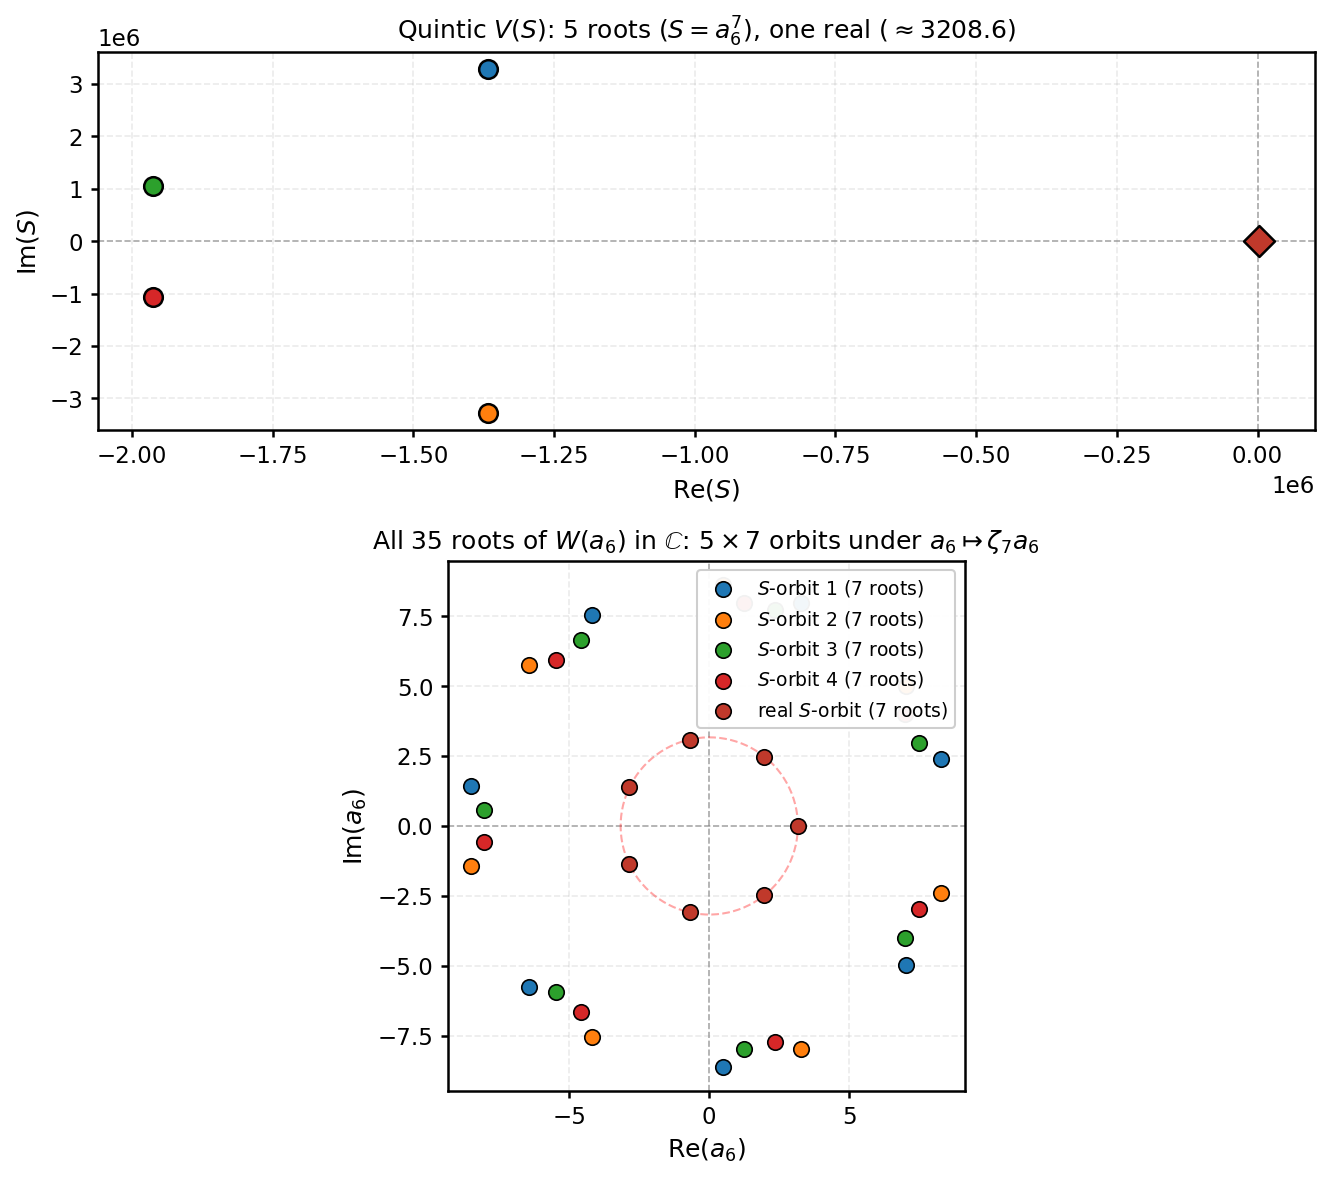
\includegraphics[width=0.85\linewidth]{figures_ab/fig3_top_layer.png}
\caption{Top: the five roots of the quintic $V(S)$ in the complex $S$-plane, computed from its integer coefficients; the real root $S\approx3208.61$ is marked with a diamond. Bottom: the $35$ roots of $\mathcal{W}(a_6)$ in $\mathbb{C}$, colored by $S$-orbit; each $S\neq0$ lifts to $7$ values of $a_6$ through the seventh roots of unity. The dashed circle marks the real $S$-orbit. The $35$ roots form a single Galois orbit over $\mathbb{Q}$.}
\label{ab:fig:top}
\end{figure}

\begin{proof}
(i) is a direct factorization in {\sc Singular} over $\mathbb{Q}$. (ii) holds by inspection, since every exponent occurring in $\mathcal{W}$ is divisible by $7$. For (iii), the discriminant was computed exactly in {\sc SymPy} and is a nonzero integer, and a Sturm sequence gives exactly one real root. (iv) is a direct $\gcd$ computation in $\mathbb{F}_{101}[a_6]$. Since $\mathcal{W}$ has integer coefficients and is squarefree modulo $101$, it is squarefree over $\mathbb{Q}$, which gives the distinctness; irreducibility gives the single Galois orbit. A real root $a_6$ of $\mathcal{W}$ has $a_6^7$ real, so $a_6^7$ is the real root of $V$ and $a_6$ is its unique real seventh root; this accounts for one real solution and $34/2=17$ conjugate pairs.
\end{proof}

\begin{remark}[Consistency of the characteristic-zero and modular routes]
Reducing the integer quintic $V$ modulo $101$ gives $58$ times the quintic obtained directly from the Gr\"obner computation modulo $101$. Equivalently the modular quintic is $54$ times $V$ modulo $101$, since $58\cdot54=3132=31\cdot101+1$.
\end{remark}

\subsection{An algebraic proof of the top-layer classification for \texorpdfstring{$m=7$}{m=7}, and its formalization}\label{ab:sec:chartproof}

The proof of Proposition~\ref{ab:prop:top-class} rests on Riemann's existence theorem, which is not available in Mathlib (at least not in the version pinned by the artifact). For $m=7$ we now give a second proof of the classification in the normalized chart of~\S\ref{ab:sec:normalization}: every solution is one of the points $(P_j(w),Q_k(w))$ with $R(w)=0$, the five $K_5$-conjugates. This is the form in which the main theorem uses Proposition~\ref{ab:prop:top-class}. The eliminant $\mathcal{W}$ and the cases $m=3,5$ are not reproved here. The proof is purely algebraic, valid over every field of characteristic~$0$, and formalized: Theorem~\ref{ab:thm:chartclass} is the Lean theorem \texttt{chartClassification\_\allowbreak{}holds} (listing~\ref{ab:lst:proofchartclass}). We use the Lean chart: $\alpha=1+a_1u+\dots+a_7u^7$, $\beta=b_0+b_1u+\dots+b_9u^9+u^{10}$, and $E_n=\sum_{i+k=n}(1+2k-3i)\,a_ib_k$ for $1\le n\le 16$ is the coefficient of $u^n$ in $\alpha\beta+u(2\alpha\beta'-3\alpha'\beta)$, with $a_0=b_{10}=1$.

\begin{theorem}[\texttt{chartClassification\_\allowbreak{}holds}]\label{ab:thm:chartclass}
Let $L$ be a field of characteristic~$0$. Suppose that $(a_1,\dots,a_7,b_0,\dots,b_9)\in L^{17}$ satisfies $E_1=\dots=E_{16}=0$ and $a_7^3b_0^2=1$. Then $(a_j,b_k)=(P_j(w),Q_k(w))$ for some root $w\in L$ of $R$, where $P_j,Q_k\in\mathbb{Q}[w]$ are the coordinates displayed in listing~\ref{ab:lst:def-chartclass}.
\end{theorem}

\begin{proof}
\emph{Step 1: reversed coordinates.} The idea is to read $\alpha$ and $\beta$ from their top ends, where the Davenport--Stothers equation becomes a statement about a square root of a power series. Since $a_7^3b_0^2=1$, we have $a_7\neq0$. Put $y_i=a_{7-i}/a_7$ for $1\le i\le 6$ and $y_7=1/a_7$, and give $y_i$ the weight~$i$. Define $S_k\in\mathbb{Q}[y_1,\dots,y_7]$, weighted homogeneous of weight~$k$, by the power series
\[
(1+y_1v+\dots+y_7v^7)^{3/2}=\sum_{k\ge0}S_k\,v^k .
\]
We derive a recursion for $S_k$. Let $F=1+\sum_iy_iv^i$ and $G=F^{3/2}=\sum_kS_kv^k$. Differentiating $G^2=F^3$ gives $2GG'=3F^2F'$, and dividing by $G=F^{3/2}$ gives $2FG'=3F'G$. The coefficient of $v^{k-1}$ on the left is $\sum_{i\ge0}2(k-i)\,y_iS_{k-i}$ (with $y_0=1$), and on the right it is $\sum_{i\ge1}3i\,y_iS_{k-i}$. Moving the terms with $i\ge1$ to one side,
\[
2kS_k=\sum_{i=1}^{7}\bigl(3i-2(k-i)\bigr)\,y_iS_{k-i}=\sum_{i=1}^{7}(5i-2k)\,y_i\,S_{k-i},\qquad S_0=1 .
\]
Now reverse $\beta$ as well: write $\tilde\beta_k=b_{10-k}$ for $0\le k\le 10$ (so $\tilde\beta_0=1$) and $\tilde\beta_k=0$ for $k>10$; in both recursions terms with a negative index are zero. We reindex $E_{17-k}$ by $i\mapsto 7-i$, $k\mapsto 10-k$. A term $a_{7-i}b_{10-j}$ with $i+j=k$ occurs in $E_{17-k}$ with coefficient $1+2(10-j)-3(7-i)=3i-2j=5i-2k$, and $a_{7-i}=a_7y_i$ (with $y_0=1$). Dividing by $a_7$,
\[
E_{17-k}/a_7=-2k\,\tilde\beta_k+\sum_{i=1}^{7}(5i-2k)\,y_i\,\tilde\beta_{k-i}\qquad(1\le k\le 16).
\]
This is the recursion for $S_k$. For $1\le k\le10$ the equations $E_{17-k}=0$ and induction on $k$ give $b_{10-k}=\tilde\beta_k=S_k(y)$. For $11\le k\le16$ we have $\tilde\beta_k=0$, and the same induction gives $0=2kS_k$, that is, $S_k(y)=0$. Finally $b_0=S_{10}(y)$, so $a_7^3b_0^2=1$ becomes $S_{10}(y)^2=a_7^{-3}=y_7^3$. Altogether
\begin{equation}\label{ab:eq:Ssystem}
S_{11}(y)=\dots=S_{16}(y)=0,\qquad S_{10}(y)^2=y_7^3 .
\end{equation}
In the language of~\S\ref{ab:sec:top}, the reversed $\beta$ is the truncation of the power-series square root of the reversed $\alpha^3/a_7^3$. This is the Davenport--Stothers condition.

\emph{Step 2: the orbit relations.} Consider the six weighted-homogeneous relations
\begin{align*}
y_4&=\tfrac{2431}{18240}y_1^4-\tfrac{1027}{1710}y_1^2y_2+\tfrac{143}{380}y_2^2+\tfrac{41}{60}y_1y_3,\\
y_5&=\tfrac{1154351}{25313472}y_1^5-\tfrac{3833107}{18985104}y_1^3y_2+\tfrac{6512}{43947}y_1y_2^2+\tfrac{24449}{166536}y_1^2y_3,\\
y_6&=\tfrac{4206749569}{4242031637760}y_1^6+\tfrac{8589189473}{1590761864160}y_1^4y_2-\tfrac{440013827}{9819517680}y_1^2y_2^2\\&\qquad+\tfrac{7454351}{734423760}y_1^3y_3+\tfrac{253}{5054}y_2^3,\\
y_7&=-\tfrac{4539711243127}{16353031963564800}y_1^7+\tfrac{13373800868041}{6132386986336800}y_1^5y_2-\tfrac{214713769679}{37854240656400}y_1^3y_2^2\\&\qquad+\tfrac{81661753}{707800898700}y_1^4y_3+\tfrac{92333}{19483170}y_1y_2^3,\\
y_2y_3&=\tfrac{3738317}{46630080}y_1^5-\tfrac{16882087}{34972560}y_1^3y_2+\tfrac{115021}{161910}y_1y_2^2+\tfrac{2277881}{5828760}y_1^2y_3,\\
y_3^2&=\tfrac{740761013029}{10605079094400}y_1^6-\tfrac{754440973541}{1988452330200}y_1^4y_2+\tfrac{3827878261}{8182931400}y_1^2y_2^2\\&\qquad+\tfrac{137816863}{918029700}y_1^3y_3+\tfrac{289}{12635}y_2^3 .
\end{align*}
Write each of them as $g=0$, with $g$ the difference of the two sides. Each satisfies
\[
y_7^3\cdot g\in(S_{11},\dots,S_{16})\subset\mathbb{Q}[y_1,\dots,y_7],
\]
with explicit cofactors of $341$ to $694$ terms whose numerators and denominators have at most $42$ digits. Since $y_7\neq0$, every solution of~\eqref{ab:eq:Ssystem} satisfies all six relations.

The relations were found by exact interpolation on the $K_5$ point, as all the weighted-homogeneous forms of weight at most~$7$ that vanish on the five orbits, and the cofactors come from exact weighted-homogeneous linear algebra over $\mathbb{Q}$. Let $(g)$ be the ideal generated by the six relations. A Gr\"obner computation over $\mathbb{Q}$ (\filename{saturation\_check.py}) shows that $(S_{11},\dots,S_{16})\subseteq(g)$ and $(g):y_7=(g)$. Together with the certificates this gives
\[
(S_{11},\dots,S_{16}):y_7^\infty=(S_{11},\dots,S_{16}):y_7^3=(g).
\]
The ideal $(g)$ has Krull dimension~$1$ and needs all six generators. It has exactly five solutions in the chart $y_1=1$ and none with $y_1=0$ other than $y=0$, in agreement with the weighted B\'ezout count $4\cdot5\cdot5\cdot6\cdot6\cdot7/7!=25200/5040=5$. These facts explain the choice of relations but are not used in the proof.

\emph{Step 3: a resultant.} The relation for $y_7$ shows $y_7\in y_1\,\mathbb{Q}[y_1,y_2,y_3]$, so $y_1\neq0$. By weighted homogeneity we may divide by powers of $y_1$: put $t=y_2/y_1^2$ and $s=y_3/y_1^3$. Substituting $y_2=ty_1^2$ and $y_3=sy_1^3$ into the relation for $y_2y_3$ and dividing by $y_1^5$ gives
\[
(t-c)\,s=N(t),\qquad c=\tfrac{2277881}{5828760},\quad N(t)=\tfrac{3738317}{46630080}-\tfrac{16882087}{34972560}\,t+\tfrac{115021}{161910}\,t^2 .
\]
The same substitution in the relation for $y_3^2$, divided by $y_1^6$, gives a monic quadratic equation in~$s$. The Sylvester resultant of the two equations with respect to $s$ is $\kappa\,m(t)$ with $\kappa\in\mathbb{Q}^\times$ and
\[
\begin{aligned}
m(t)={}&287548593020928\,t^5-688401965085696\,t^4+640652914818432\,t^3\\
&-292066554895024\,t^2+65563255857792\,t-5817852446211,
\end{aligned}
\]
which is irreducible over $\mathbb{Q}$. Since $m(c)\neq0$, the element $t-c$ is invertible modulo~$m$, and $s=q_3(t)$ for a polynomial $q_3\in\mathbb{Q}[t]$ reduced modulo~$m$. The first four relations then give $y_i/y_1^i=q_i(t)$ for $4\le i\le 7$, again with $q_i\in\mathbb{Q}[t]$ reduced modulo~$m$.

\emph{Step 4: the torus.} Let $z=1/y_1$. By weighted homogeneity, scaling each $y_i$ by $z^i$ multiplies a form of weight $k$ by $z^k$, so
\[
z^{10}S_{10}(y)=S_{10}\bigl(1,t,q_3(t),\dots,q_7(t)\bigr)\equiv\sigma(t)\pmod m\qquad\text{and}\qquad z^7y_7=q_7(t).
\]
Multiplying $S_{10}^2=y_7^3$ by $z^{21}$, the left side becomes $z\cdot\bigl(z^{10}S_{10}\bigr)^2=z\,\sigma(t)^2$ and the right side becomes $(z^7y_7)^3=q_7(t)^3$. Hence $z\,\sigma(t)^2=q_7(t)^3$, that is,
\[
y_1=\sigma(t)^2\,q_7(t)^{-3}\bmod m(t).
\]
This fixes the torus without a seventh root, as in~\S\ref{ab:sec:normalization}, and makes every $y_i$ a polynomial in $t$ modulo~$m$. The substitution $w=\omega(t)$, with $\omega\in\mathbb{Q}[t]$ of degree~$4$, induces an isomorphism $\mathbb{Q}[t]/(m)\cong\mathbb{Q}[w]/(R)=K_5$ and gives $R(w)=0$ and $y_i=Y_i(w)$.

\emph{Step 5: back to the chart.} The formulas $a_7=1/y_7$ and $a_{7-i}=y_i/y_7$, together with the recursion of Step~1 for $b_{10-k}$, give $a_j=P_j(w)$ and $b_k=Q_k(w)$.
\end{proof}

\begin{lemma}[Transfer to characteristic zero]\label{ab:lem:chart-transfer}
Let $F$ be a field of characteristic~$0$. Every $F$-valued solution of the normalized $m=7$ chart system is obtained by specializing the $K_5$-point at a root $w\in F$ of $R$. Over a splitting field of $R$, the five specializations at the five roots of $R$ are the five solutions.
\end{lemma}

\begin{proof}
Steps~1--5 are algebraic identities over $\mathbb{Q}$, so they hold over every field of characteristic zero by base change; the Lean formalization quantifies over all fields $L$ with \texttt{CharZero}. The five solutions are the $K_5$-conjugates $(P_j(w),Q_k(w))$ with $R(w)=0$.
\end{proof}

\begin{remark}[Roles of the two classifications]
The $m=7$ case of Proposition~\ref{ab:prop:top-class} is proved twice. The Belyi route combines the geometric upper bound (at most $35$ chart points over $\mathbb{C}$) with the $35$ points exhibited by the msolve parametrization, and so gives a complete classification in characteristic~$0$; it depends on Riemann's existence theorem and on the computed parametrization. The algebraic certificate of this section gives an independent classification: every solution in characteristic~$0$ lies in one of the five $K_5$-orbits (Lemma~\ref{ab:lem:chart-transfer}). Lean's \texttt{main\_\allowbreak{}theorem} uses only the algebraic route.
\end{remark}

\begin{remark}[Formalization]\label{ab:rem:chartproof-lean}
The proof is formalized in \filename{lean/Jacobian/ChartProof/}, in $12$ modules. All of them are generated by \filename{lean/certgen/chartproof/} except the hand-written \filename{Reflect.lean}.

The formal proof has $111$ steps. In $105$ of them a polynomial $g$ is shown to vanish because $g=\sum_i c_ie_i$ for polynomials $e_i$ already known to vanish. In the other six, one for each relation of Step~2, the identity $y_7^3\,g=e$ holds with $e$ already known to vanish, and $y_7^3$ is cancelled using $y_7\neq0$.

Every identity is checked by the Lean kernel. The theorem \texttt{lc\_\allowbreak{}zero} (listing~\ref{ab:lst:lczero}) and the lemma \texttt{eq\_\allowbreak{}of\_\allowbreak{}toPolyK} reduce each identity to an equality of normal forms. The normal forms are computed by the verified normalizer of \texttt{Lean.\allowbreak{}Grind.\allowbreak{}CommRing} from Lean core, with a kernel-friendly multiplication defined by recursors (\texttt{toPolyK}, with soundness theorem \texttt{denote\_\allowbreak{}toPolyK}), and \texttt{decide +kernel} evaluates them. No \texttt{native\_\allowbreak{}decide} is used, and \texttt{\#print axioms} for \texttt{chartClassification\_\allowbreak{}holds} and for \texttt{main\_\allowbreak{}theorem} reports only \texttt{propext}, \texttt{Classical.\allowbreak{}choice} and \texttt{Quot.\allowbreak{}sound}.

The certificates of Step~2 have between $27{,}747$ and $56{,}999$ monomial products each. They are split into batches of at most $9{,}000$ products, one declaration per batch.

Every certificate was also verified by exact {\sc SymPy} expansion before it was written, and the generator reproduces all eleven generated modules byte for byte. A second checker, written independently of the generator (\filename{independent\_check.py}), parses the Lean text and re-verifies all $111$ identities over $\mathbb{Z}$. This checker verifies the arithmetic of the certificates only and does not re-prove the mathematical statements; the Lean kernel alone is responsible for checking that the certificates prove the stated propositions. Six controls behave as expected: four perturbations of a single integer are rejected by \texttt{decide}, a planted \texttt{sorry} is flagged, and an unmodified module is accepted. The build takes about $25$ minutes sequentially and needs at most $5.4$\,GB of memory for any one module.
\end{remark}

\begin{remark}[Why these coordinates]
Earlier formulations failed to give certificates of practical size, because of the degenerate Davenport--Stothers components of lower degree (the solutions for $m=1,3,5$). With $a_0=b_0=1$ and $b$ eliminated, these components force saturation by $a_7^7$ or $a_7^8$, and the certificates have weight~$61$. In the chart $a_0=b_{10}=1$ the sub-case $a_1=0$ alone needed $503{,}254$ cofactor terms modulo a prime. Replayed over~$\mathbb{Q}$, its Buchberger trace reached coefficients of $2{,}722$ digits after $929$ of its $2{,}065$ elements (\filename{lean/CLASSIFICATION\_STATUS.md}, \S5). In the reversed coordinates the same components lie on $y_7=0$, so $y_7^3$ suffices, at weight at most~$28$, and the five orbits form a weighted complete intersection that can be written down explicitly. The six certificates of Step~2 have $341$ to $694$ cofactor terms each over~$\mathbb{Q}$, roughly a thousand times fewer than the modular lift for $a_1=0$ alone.
\end{remark}

% keep the caption of the next listing on the same page as its code
\par\vskip 0pt plus 8\baselineskip\penalty-200\vskip 0pt plus -8\baselineskip\relax
% BEGIN-MECHANICAL:lst:proofchartclass
\begin{leanlisting}{Mechanically extracted from \texttt{Jacobian/ChartProof/Final.lean} (sha256 \texttt{638b644ffb58cb8b}); statement verbatim, proof elided.}{ab:lst:proofchartclass}
theorem chartClassification_holds (L : Type*) [Field L] [CharZero L] : ChartClassification L := by
  -- proof body elided (see artifact)
\end{leanlisting}
% END-MECHANICAL:lst:proofchartclass
% BEGIN-MECHANICAL:lst:unconditional
\begin{leanlisting}{Mechanically extracted from \texttt{Jacobian/ChartProof/Final.lean} (sha256 \texttt{638b644ffb58cb8b}); statement verbatim, proof elided.}{ab:lst:unconditional}
theorem main_theorem {L : Type*} [Field L] [CharZero L] :
    ¬ exists (P Q : MvPolynomial (Fin 2) L) (lam : L), lam ≠ 0 /\ NewtonNF2 P Q /\ jac P Q = MvPolynomial.C lam * MvPolynomial.X 0 ^ 2 :=
  -- proof term elided (see artifact)
\end{leanlisting}
% END-MECHANICAL:lst:unconditional
% BEGIN-MECHANICAL:lst:lczero
\begin{leanlisting}{Mechanically extracted from \texttt{Jacobian/ChartProof/Reflect.lean} (sha256 \texttt{9e3ea428ffe7236b}); statement verbatim, proof elided.}{ab:lst:lczero}
theorem lc_zero (ctx : Context α) (g : Expr) (l : List (Expr × Expr))
    (hcert : Poly.beq' (toPolyK (.sub g (lcExpr l))) (.num 0) = true) (h : AllZero ctx l) :
    g.denote ctx = 0 := by
  -- proof body elided (see artifact)
\end{leanlisting}
% END-MECHANICAL:lst:lczero

\section{Descent}\label{ab:sec:descent}

Fix a top-layer solution $(\alpha,\beta)$; by Proposition~\ref{ab:prop:top-class} and the torus we may take it to be the $K_5$ point. We keep the scaled variables $A_2=u\alpha$ and $B_3=u^2\beta$, and we solve $E_4$, $E_3$, $E_2$ in turn. In each layer the new unknowns enter linearly, so each step is a question about the rank of one coefficient matrix.

\subsection{\texorpdfstring{Layer $E_4$}{Layer E4}}

In $E_4$, $2(A_2B_2'-A_2'B_2)+(A_1B_3'-3A_1'B_3)=0$, the known polynomials $A_2,B_3$ multiply the unknowns $A_1$ and $B_2$, and there is no inhomogeneous term.

\begin{proposition}[$E_4$ structure]\label{ab:prop:e4}
$E_4$ is a homogeneous linear system in $19$ unknowns ($A_1$ on $u^1,\dots,u^8$ and $B_2$ on $u^2,\dots,u^{12}$) with $18$ equations, of rank $17$, so its kernel has dimension $19-17=2$. The kernel is parametrized by $t=(t_1,t_2)$, giving $(A_1(t),B_2(t))$ linear in $t$. This is computed exactly over the quintic field $K_5=\mathbb{Q}[w]/(w^5-w^4+3w^3+3w^2+26)$ (script \filename{exact\_ranks\_K5.py}); a modular evaluation at $p=101$, $a_6=55$, is an independent cross-check.
\end{proposition}

\begin{proof}
The rank is computed on the $18\times19$ coefficient matrix, with residual assertions verifying the kernel. The scripts are \filename{exact\_ranks\_K5.py} (exact rank and kernel over $K_5$) and \filename{C5\_E2\_obstruction\_corrected.py} (which verifies that the $E_4$ kernel residuals are zero, with the cross-check modulo~$101$).
\end{proof}

\subsection{\texorpdfstring{Layer $E_3$}{Layer E3}}

In $E_3$ the unknowns are $A_0$ and $B_1$, which enter through $\mathrm{LT}_{2,1}(A_2,B_1)+\mathrm{LT}_{0,3}(A_0,B_3)=2A_2B_1'-A_2'B_1-3A_0'B_3$. The remaining term $\mathrm{LT}_{1,2}(A_1(t),B_2(t))$ is known once $t$ is chosen, and it is quadratic in $t$ because both arguments are linear in $t$. Since $A_0$ enters only through $A_0'$, its constant term $a_{0,0}$ drops out, and we take as unknowns the coefficients of $A_0$ on $u^1,\dots,u^8$ (with $a_{8,16}$ free) and of $B_1$ on $u^1,\dots,u^{12}$, $20$ in all.

\begin{proposition}[$E_3$ structure and unconditional solvability]\label{ab:prop:e3}
$E_3$ is a $19\times20$ linear system of rank $18$, with $2$-dimensional kernel. It is solvable for every direction $t=(t_1,t_2)$. Write the system as $Mx=K(t)$, with $M$ constant and $K(t)=t_1^2K_{11}+t_1t_2K_{12}+t_2^2K_{22}$ quadratic in $t$, and let $v$ be the left null vector, $v^{\mathrm{T}}M=0$. Then
\begin{equation}
v^{\mathrm{T}} K_{11}=0,\qquad v^{\mathrm{T}} K_{22}=0,\qquad v^{\mathrm{T}} K_{12}=0,
\end{equation}
so the compatibility condition $v^{\mathrm T}K(t)=0$ holds identically in $t$, and no direction is obstructed at $E_3$. All computations are exact over $K_5$; see Lemma~\ref{ab:lem:lifting}(i).
\end{proposition}

\begin{proof}
The $19\times20$ matrix $M$ has rank $18$, so its left null space has dimension $19-18=1$ and is spanned by $v$. Splitting the inhomogeneous part into its three quadratic pieces and computing each $v^{\mathrm{T}}K_{ij}$ gives zero. The script is \filename{C5\_E2\_obstruction\_corrected.py}, which verifies $E_3$ with residual assertions.
\end{proof}

The general solution of $E_3$ is thus the $2$-parameter affine family
\begin{equation}
x(t,s)=t_1^2x_{11}+t_1t_2x_{12}+t_2^2x_{22}+s_1w_1+s_2w_2,
\end{equation}
where $x_{ij}$ are particular solutions for the three quadratic pieces and $w_1,w_2$ span the kernel. It encodes $(A_0,B_1)$ in terms of $(t,s)=(t_1,t_2,s_1,s_2)\in\mathbb{C}^4$. Both kernel directions move actual coefficients.

\subsection{\texorpdfstring{Layer $E_2$}{Layer E2}}

In $E_2$, $2A_2B_0'+(A_1B_1'-A_1'B_1)-2A_0'B_2=0$, the only new unknown is $B_0$, and it enters only through the term $2A_2B_0'$.

\begin{proposition}[$E_2$ injectivity]\label{ab:prop:e2}
The homogeneous operator of $E_2$ in the unknown $B_0'$ is a $19\times12$ matrix of rank $12$, hence injective. Its left null space has dimension $19-12=7$. This is exact over $K_5$; see Lemma~\ref{ab:lem:lifting}(i)--(ii).
\end{proposition}

The sizes can be read off directly. $B_0'$ has the $12$ coefficients of $u^0,\dots,u^{11}$, and the operator is $B_0'\mapsto 2A_2B_0'$, whose values live on $u^1,\dots,u^{19}$ because $A_2$ is supported on $u^1,\dots,u^8$; this gives $19$ rows. Multiplication by the nonzero polynomial $2A_2$ is injective on $K[u]$, which explains the rank $12$. Therefore $B_0'$, and hence $B_0$ up to an additive constant, is uniquely determined by $(A_0,B_1,A_1,B_2)$. The seven left null vectors then give seven compatibility conditions,
\begin{equation}\label{ab:eq:seven}
W\cdot\mathrm{rhs}(t,s)=0,
\end{equation}
where the rows of the $7\times19$ matrix $W$ span the left null space and $\mathrm{rhs}(t,s)=-(A_1B_1'-A_1'B_1)+2A_0'B_2$ is the inhomogeneous term of $E_2$, written as a vector of $19$ coefficients. These seven conditions are the only remaining obstructions; $E_1$ is never needed for Theorem~\ref{ab:thm:main}.

% BEGIN-MECHANICAL:lst:descent
\begin{leanlisting}{Mechanically extracted from \texttt{Jacobian/Descent/Main.lean} (sha256 \texttt{e18a3a9e531df6d6}); statement verbatim, proof elided.}{ab:lst:descent}
theorem descent_K5 {L : Type*} [Field L] [CharZero L]
    (w : L)
    (hw : w ^ 5 - w ^ 4 + 3 * w ^ 3 + 3 * w ^ 2 + 26 = 0)
    (a_1_0 a_2_2 a_3_4 a_4_6 a_5_8 a_6_10 a_7_12 a_8_14 b_2_1 b_3_3 b_4_5 b_5_7 b_6_9 b_7_11 b_8_13 b_9_15 b_10_17 b_11_19 b_12_21 : L)
    (h_a_1_0 : a_1_0 = ((1 : L)))
    -- ... (18 h4_*, 19 h3_*, 19 h2_*, 8 h_a_*, 11 h_b_*, 51 lower-layer unknowns in one binder)
    (hv : b_12_24 ≠ 0) :
    False := by
  -- proof body elided (see artifact)
\end{leanlisting}
% END-MECHANICAL:lst:descent

\section{The final obstruction}\label{ab:sec:obstruction}

We use the homogeneous formulation of $E_3$ described above: $A_0$ on $u^1,\dots,u^8$ with $a_{8,16}$ free and no constant term, and $B_1$ on $u^1,\dots,u^{12}$. It gives the genuine $2$-dimensional kernel, with two independent directions $s=(s_1,s_2)$ that both move actual coefficients. (An earlier formulation froze $a_{8,16}=1$ and included the constant term as an unknown; the constant is killed by $A_0'$ and contributes only a trivial direction.)

\begin{remark}[Free parameter]
Section~\ref{ab:sec:normalization} leaves $a_{8,16}$ free from the start. The analysis of $E_2$ and $E_3$ therefore applies to every slice, including $a_{8,16}=1$, without a superset argument.
\end{remark}

\subsection{Explicit form of the seven conditions}

Before expanding~\eqref{ab:eq:seven}, we determine its shape. By Proposition~\ref{ab:prop:e4}, $A_1$ and $B_2$ are linear in $t$. By the family $x(t,s)$, $A_0$ and $B_1$ are sums of a part quadratic in $t$ and a part linear in $s$. In $\mathrm{rhs}(t,s)$ every term is a product of one factor from $\{A_1,B_2\}$ and one from $\{A_0,B_1\}$, so it is a sum of a part cubic in $t$ and a part bilinear in $t$ and~$s$.

\begin{lemma}\label{ab:lem:seven-explicit}
Each of the seven conditions has the form
\begin{equation}
b_i(t_1,t_2)+s_1\,M_i(t_1,t_2)+s_2\,L_i(t_1,t_2)=0,\qquad i=1,\dots,7,
\end{equation}
where $b_i$ is a homogeneous cubic and $M_i$, $L_i$ are linear forms in $(t_1,t_2)$. Both $s_1$ and $s_2$ occur with nonzero coefficient.
\end{lemma}

\begin{proof}
The shape follows from the remark above. The coefficients come from an exact expansion over $K_5$ in python-flint (script \filename{exact\_obstruction\_K5.py}) of $W\cdot\mathrm{rhs}(t,s)$ with the homogeneous $E_3$ parametrization $x(t,s)=t_1^2x_{11}+t_1t_2x_{12}+t_2^2x_{22}+s_1w_1+s_2w_2$ substituted. The {\sc SymPy} expansion over $\mathbb{F}_{101}$ (script \filename{C5\_E2\_obstruction\_corrected.py}) is a cross-check.
\end{proof}

\subsection{\texorpdfstring{Elimination of $(s_1,s_2)$}{Elimination of (s1,s2)}}

For fixed $t\neq0$ the seven equations are affine-linear in $(s_1,s_2)$: they say that the column $b(t)$ is a linear combination of the columns $M(t)$ and $L(t)$. Then the $7\times3$ matrix $[b(t)\mid M(t)\mid L(t)]$ has rank at most $2$, so all its $3\times3$ minors vanish:
\begin{equation}\label{ab:eq:minors}
\det\begin{pmatrix}
b_i & M_i & L_i \\ b_j & M_j & L_j \\ b_k & M_k & L_k
\end{pmatrix}=0,\qquad 1\leq i<j<k\leq7.
\end{equation}
There are $\binom{7}{3}=35$ such minors. Expanding along the first column, each is a sum of products of a cubic, a linear and a linear form, hence a homogeneous binary quintic in $(t_1,t_2)$.

\begin{theorem}[No nonzero direction]\label{ab:thm:no-direction}
The $35$ quintics~\eqref{ab:eq:minors} span the space $K_5[t_1,t_2]_5$ of binary quintics, and they generate the ideal $(t_1,t_2)^5$; that is, exactly over $K_5$ they have the Gr\"obner basis
\begin{equation}
(t_1,t_2)^5 = \left\{\, t_1^5,\; t_1^4 t_2,\; t_1^3 t_2^2,\; t_1^2 t_2^3,\; t_1 t_2^4,\; t_2^5 \,\right\}.
\end{equation}
Hence their common projective zero locus is empty, and their only common zero in $\overline{K_5}^2$ is $(0,0)$: no nonzero $t$ admits $(s_1,s_2)$ satisfying the seven $E_2$ conditions. A Gr\"obner computation modulo $101$ (lexicographic order) is an independent cross-check.
\end{theorem}

\begin{proof}
The space of binary quintics has the basis $t_1^5,t_1^4t_2,\dots,t_2^5$, so it has dimension~$6$. Writing the $35$ minors in this basis gives a $35\times6$ coefficient matrix, which has rank~$6$ over $K_5$. Hence
\[
\operatorname{span}_{K_5}\{M_{ijk}\}=K_5[t_1,t_2]_5 .
\]
So every monomial of degree five lies in the ideal $I$ generated by the minors, that is, $(t_1,t_2)^5\subseteq I$. Conversely each generator is a quintic and lies in $(t_1,t_2)^5$, so $I=(t_1,t_2)^5$. Its radical is $(t_1,t_2)$, so the affine variety over the algebraic closure is $\{(0,0)\}$. The script \filename{exact\_obstruction\_K5.py} also writes the $35\times6$ matrix and a nonzero $6\times6$ minor to \filename{logs/k5\_minor\_certificate.json} as a machine-readable certificate. The {\sc SymPy} Gr\"obner basis over $GF(101)$ (script \filename{C5\_E2\_obstruction\_corrected.py}, saved and rerunnable, log archived) is a cross-check.
\end{proof}

\begin{remark}[Interpretation]
The top layer admits five orbits in characteristic zero, but none extends to a full solution. The $E_4$ kernel gives a two-dimensional space of directions $t\in K^2$, the layer $E_3$ imposes no further restriction, and the seven $E_2$ compatibility conditions then force $t=0$ through the $35$ quintic minors. The remaining case $t=0$ is ruled out separately (Corollary~\ref{ab:cor:t0}). In other words, the top-layer solutions exist in isolation, but none extends to a Newton normal-form pair with $[P,Q]=\lambda x^2$.
\end{remark}

\subsection{\texorpdfstring{The case $t=0$}{The case t=0}}\label{ab:sec:t0}

\begin{lemma}[Collapse at $t=0$]\label{ab:lem:t0-collapse}
At $t=(0,0)$ the layer equation $E_2$ reduces to $2A_2B_0'=0$.
\end{lemma}
\begin{proof}
The target $\lambda x^2=\lambda u^2y^{-4}$ has only a $y^{-4}$ component, so the layer equation $E_4$, the $y^{-3}$ component, is homogeneous:
\[
2(A_2B_2'-A_2'B_2)+(A_1B_3'-3A_1'B_3)=0.
\]
Its solutions are the linear family $(A_1(t),B_2(t))$ of Proposition~\ref{ab:prop:e4}, so $t=(0,0)$ forces $(A_1,B_2)=(0,0)$. In $E_3$ the quadratic driving term $K(t)$ then vanishes, leaving only the homogeneous kernel. In $E_2$, the terms $(A_1B_1'-A_1'B_1)-2A_0'B_2$ each contain a factor $A_1$ or $B_2$ and vanish, which leaves $2A_2B_0'=0$.
\end{proof}

\begin{corollary}[$t=0$ is impossible]\label{ab:cor:t0}
At $t=0$ we have $2A_2B_0'=0$ by Lemma~\ref{ab:lem:t0-collapse}. Since $A_2=u\alpha\neq0$ and $K[u]$ is a domain, $B_0'=0$, and $B_0(u)$ is constant. The coefficient of $u^{11}$ in $B_0'$ is $12\,b_{12,24}$, so $b_{12,24}=0$; in particular $(12,24)$ cannot be a vertex of $N(Q)$.
\end{corollary}

This argument uses $2\neq0$ and $12\neq0$, so it is valid in every characteristic other than $2$ and $3$.

\begin{remark}
The Lean theorem \texttt{e2\_\allowbreak{}t0} (listing~\ref{ab:lst:t0}) proves $b_{12,24}=0$ by a different route: a left-inverse certificate on the reduced $E_2$ equations, with $t=0$ supplied as hypotheses, rather than the argument above. Both routes reach the same conclusion.
\end{remark}

% BEGIN-MECHANICAL:lst:t0
\begin{leanlisting}{Mechanically extracted from \texttt{Jacobian/Descent/E2/T0.lean} (sha256 \texttt{3559bcbdbff42d3c}); statement verbatim, proof elided.}{ab:lst:t0}
theorem e2_t0 {L : Type*} [Field L] [CharZero L]
    (w : L)
    (hw : w ^ 5 - w ^ 4 + 3 * w ^ 3 + 3 * w ^ 2 + 26 = 0)
    (b_11_20 b_12_22 b_11_21 b_12_23 b_1_2 b_2_4 b_3_6 b_4_8 b_5_10 b_6_12 b_7_14 b_8_16 b_9_18 b_10_20 b_11_22 b_12_24 : L)
    -- 19 reduced E2 equations (r2_1_1) ... (r2_19_37), hypotheses elided for brevity
    (ht1 : b_11_20 = 0)
    (ht2 : b_12_22 = 0) :
    b_12_24 = 0 := by
  -- proof body elided (see artifact)
\end{leanlisting}
% END-MECHANICAL:lst:t0

\subsection{Proof of the main theorem}

\begin{proof}[Proof of Theorem~\ref{ab:thm:main}]
By Proposition~\ref{ab:prop:layers} the layers satisfy the equations $E_5,\dots,E_1$. Since $a_{1,0}\,a_{8,14}\,b_{2,1}\,b_{12,21}\neq 0$, Proposition~\ref{ab:prop:top-class} puts $(A_2,B_3)$ in the torus orbit of the $K_5$ point for some root $w$ of $R$, and by torus transport (listing~\ref{ab:lst:torus}) we may take it to be that point. Propositions~\ref{ab:prop:e4}--\ref{ab:prop:e2} and Theorem~\ref{ab:thm:no-direction} force $t=0$. At $t=0$, Lemma~\ref{ab:lem:t0-collapse} and Corollary~\ref{ab:cor:t0} give $B_0'=0$, so $b_{12,24}=0$ (in Lean, \texttt{e2\_\allowbreak{}t0}, listing~\ref{ab:lst:t0}). The last sentence of the theorem follows because $\mathrm{NewtonNF2}$ requires $b_{12,24}\neq 0$.
\end{proof}

\begin{proof}[Proof of Corollary~\ref{ab:cor:a816}]
As in the proof of Theorem~\ref{ab:thm:main} we may take the top layer to be the $K_5$ point, where $E_4$, $E_3$, $E_2$ force $t=0$; torus transport multiplies each coefficient by a nonzero scalar. At $t=0$ we have $A_1=B_2=0$ (Proposition~\ref{ab:prop:e4}). By Proposition~\ref{ab:prop:e3}, the coefficients of $A_0$ other than $a_{0,0}$, and the coefficients of $B_1$, are $K_5$-linear forms in $s=(b_{11,21},b_{12,23})$, the two free unknowns of $E_3$. In particular $a_{8,16}=\gamma\,b_{12,23}$ with $\gamma\in K_5^{\times}$, and $b_{11,21}$ occurs in $a_{1,2}$ with a nonzero coefficient. Since $A_1=0$, the layer $E_1$, $A_1B_0'-A_0'B_1=0$, reduces to $A_0'B_1=0$ in $K[u]$. Because $K[u]$ is a domain, $A_0'=0$ or $B_1=0$. If $B_1=0$, then $s=0$. If $A_0'=0$, then $a_{1,2}=a_{8,16}=0$, and again $s=0$. Hence $A_0=a_{0,0}$ and $B_1=0$; in particular $a_{8,16}=0$. Finally $B_0$ is constant by Corollary~\ref{ab:cor:t0}.

In Lean (\texttt{lower\_\allowbreak{}edge\_\allowbreak{}rigidity}, generated by \filename{lean/certgen/gen\_a816.py}) the $E_1$ step uses instead the coefficients of $x^{17}y^{34}$, $x^{18}y^{36}$ and $x^{19}y^{38}$ in $E_1$. Since $E_1$ is the weight-$0$ component, $u^n$ corresponds to $x^ny^{2n}$, and these are the coefficients of $u^{17}$, $u^{18}$, $u^{19}$. At $t=0$ they are quadratic forms in $s$ that span all three quadratic monomials, and explicit $K_5$ multipliers give $b_{12,23}^2=0$ and $b_{11,21}^2=0$. The last coefficient alone gives $a_{8,16}=0$. Indeed, only the top terms reach $u^{19}$: $A_1B_0'$ contributes $a_{8,15}u^8\cdot12\,b_{12,24}u^{11}$ and $A_0'B_1$ contributes $8\,a_{8,16}u^7\cdot b_{12,23}u^{12}$, so the coefficient of $u^{19}$ in $E_1$ is
\[
12\,a_{8,15}b_{12,24}-8\,a_{8,16}b_{12,23}.
\]
At $t=0$ we have $a_{8,15}=0$ (it is a coefficient of $A_1$) and $a_{8,16}=\gamma\,b_{12,23}$, so this coefficient equals $-8\gamma\,b_{12,23}^2$, and its vanishing gives $b_{12,23}=0$ and then $a_{8,16}=0$.

A second proof of $a_{8,16}=0$, outside Lean and independent of the descent, is an explicit certificate. At the $K_5$ point, let $e_1,\dots,e_{75}$ be the coefficients of $[P,Q]-x^2$ in the layers $E_4,\dots,E_1$, as built by \filename{scripts/a816\_full.sing}; the unknowns occurring in them are the $51$ lower coefficients of $P$ and $Q$. There is an explicit identity
\[
a_{8,16}^2=\sum_{k=1}^{75}H_k\,e_k,\qquad H_k\in K_5[a,b],
\]
stored in Rabinowitsch form, $1=\sum_k z^2H_k\,e_k-(1+a_{8,16}z)(a_{8,16}z-1)$, as the $76$ cofactors of \filename{scripts/a816\_certificate/a816\_lift.txt} ($3464$ terms, with coefficients of at most $493$ digits). (Expanding, $(1+a_{8,16}z)(a_{8,16}z-1)=a_{8,16}^2z^2-1$, so the stored identity is $z^2\bigl(\sum_kH_ke_k-a_{8,16}^2\bigr)=0$, equivalent to the displayed one.) The certificate is built from the layer structure. Give the coefficients of $A_1,B_2$ depth~$1$, those of $A_0,B_1$ depth~$2$, and those of $B_0$ depth~$3$; then each equation of $E_{5-d}$ is homogeneous of depth~$d$ and linear in the unknowns of depth~$d$. Row reduction of these linear parts in $E_4$, $E_3$, $E_2$ (ranks $17$, $18$ and $12$ over $K_5$) expresses every unknown, modulo the layer ideal, as a polynomial in four free ones: $\tau=(b_{11,20},b_{12,22})$ of depth~$1$ and $\sigma=(a_{8,16},b_{11,21})$ of depth~$2$. The $32$ products of depth~$4$ formed from the reduced generators span all $14$ monomials of depth~$4$ in $K_5[\tau,\sigma]$, and lifting back gives the $H_k$. The identity is checked exactly by {\sc Singular} over $\mathbb{Q}(w)$, and independently by python-flint, which rebuilds $[P,Q]$ from $P$ and $Q$ (\filename{scripts/a816\_certificate/verify\_bundle.sh}). Hence $a_{8,16}=0$ at the $K_5$ point once $E_1$ is included. Torus transport multiplies $a_{8,16}$ by a nonzero scalar, so $a_{8,16}=0$ on the whole orbit.
\end{proof}

\begin{remark}[Further rigidity, outside the certificate]\label{ab:rem:full-rigidity}
The same span statement puts every monomial of depth at least~$4$ in $\tau,\sigma$ into the layer ideal, so each of the $51$ unknowns (the non-constant lower coefficients of $P$ and $Q$) is nilpotent modulo that ideal. At the $K_5$ point, then, the only solution of $E_4,\dots,E_1$ is $P=P_2+\mathrm{const}$, $Q=Q_3+\mathrm{const}$. Explicitly, let $x$ be an unknown of depth~$d$, and let $p_x\in K_5[\tau,\sigma]$ be the polynomial given by the row reduction, with $x\equiv p_x$ modulo the layer ideal ($p_x=x$ for a free unknown). It is homogeneous of depth~$d$ with no constant term. So $x^{\lceil 4/d\rceil}\equiv p_x^{\lceil 4/d\rceil}$, and every monomial of $p_x^{\lceil 4/d\rceil}$ has depth $d\lceil4/d\rceil\ge4$ and is therefore divisible by a monomial of depth exactly~$4$. The certificates behind this are written out and checked exactly by two independent programs (\filename{scripts/a816\_rigidity/}): the $47$ identities $x-p_x=\sum_kD_{x,k}e_k$ for the pivot unknowns, and the $14$ identities $m=\sum_kH_{m,k}e_k$ for the monomials~$m$ of depth~$4$. The zero-set form of this statement, $P=P_2+\mathrm{const}$ and $Q=Q_3+\mathrm{const}$, is the Lean theorem \texttt{lower\_\allowbreak{}edge\_\allowbreak{}rigidity} (Corollary~\ref{ab:cor:a816}); the nilpotency modulo the layer ideal is not part of the Lean formalization. Neither is used elsewhere.
\end{remark}

% BEGIN-MECHANICAL:lst:a816
\begin{leanlisting}{Mechanically extracted from \texttt{Jacobian/A816/Final.lean} (sha256 \texttt{b7f3ed6341617a44}); statement verbatim, proof elided.}{ab:lst:a816}
theorem lower_edge_rigidity {L : Type*} [Field L] [CharZero L] (P Q : MvPolynomial (Fin 2) L) (lam : L)
    (hP : forall m ∈ P.support, inNP m) (hQ : forall m ∈ Q.support, inNQ m)
    (v10 : P.coeff (mono 1 0) ≠ 0) (v814 : P.coeff (mono 8 14) ≠ 0)
    (w21 : Q.coeff (mono 2 1) ≠ 0) (w1221 : Q.coeff (mono 12 21) ≠ 0)
    (hJ : jac P Q = MvPolynomial.C lam * MvPolynomial.X 0 ^ 2) :
    (forall i j, 2 * i ≤ j + 1 → (i, j) ≠ (0, 0) → P.coeff (mono i j) = 0) /\
      (forall k l, 2 * k ≤ l + 2 → (k, l) ≠ (0, 0) → Q.coeff (mono k l) = 0) := by
  -- proof body elided (see artifact)
\end{leanlisting}
% END-MECHANICAL:lst:a816
% BEGIN-MECHANICAL:lst:a816-nf2
\begin{leanlisting}{Mechanically extracted from \texttt{Jacobian/A816/Final.lean} (sha256 \texttt{b7f3ed6341617a44}); statement verbatim, proof elided.}{ab:lst:a816-nf2}
theorem main_theorem_lower_edge {L : Type*} [Field L] [CharZero L] :
    ¬ exists (P Q : MvPolynomial (Fin 2) L) (lam : L), lam ≠ 0 /\ NewtonNF2 P Q /\ jac P Q = MvPolynomial.C lam * MvPolynomial.X 0 ^ 2 := by
  -- proof body elided (see artifact)
\end{leanlisting}
% END-MECHANICAL:lst:a816-nf2

\begin{proof}[Proof of Corollary~\ref{ab:cor:gghv}]
Apply \cite[Proposition~4.3]{GGHV} and then Theorem~\ref{ab:thm:main}.
\end{proof}

% BEGIN-MECHANICAL:lst:main
\begin{leanlisting}{Mechanically extracted from \texttt{Jacobian/BranchAbFinal.lean} (sha256 \texttt{cd4e207adba5cb7b}); statement verbatim, proof elided.}{ab:lst:main}
theorem no_completion_K5 {L : Type*} [Field L] [CharZero L] (w : L)
    (hw : w ^ 5 - w ^ 4 + 3 * w ^ 3 + 3 * w ^ 2 + 26 = 0) (lam : L)
    (A₀ A₁ A₂ B₀ B₁ B₂ B₃ : Polynomial L) (p₀ p₁ p₂ q₀ q₁ q₂ q₃ : MvPolynomial (Fin 2) L)
    (hp₀ : X 1 ^ 0 * p₀ = evH A₀) (hp₁ : X 1 ^ 1 * p₁ = evH A₁) (hp₂ : X 1 ^ 2 * p₂ = evH A₂)
    (hq₀ : X 1 ^ 0 * q₀ = evH B₀) (hq₁ : X 1 ^ 1 * q₁ = evH B₁) (hq₂ : X 1 ^ 2 * q₂ = evH B₂)
    (hq₃ : X 1 ^ 3 * q₃ = evH B₃)
    (hJ : jac (p₀ + p₁ + p₂) (q₀ + q₁ + q₂ + q₃) = C lam * X 0 ^ 2)
    (sA₀ : forall i, A₀.coeff i ≠ 0 → 0 ≤ i /\ i ≤ 8)
    (sA₁ : forall i, A₁.coeff i ≠ 0 → 1 ≤ i /\ i ≤ 8)
    (sA₂ : forall i, A₂.coeff i ≠ 0 → 1 ≤ i /\ i ≤ 8)
    (sB₀ : forall i, B₀.coeff i ≠ 0 → 0 ≤ i /\ i ≤ 12)
    (sB₁ : forall i, B₁.coeff i ≠ 0 → 1 ≤ i /\ i ≤ 12)
    (sB₂ : forall i, B₂.coeff i ≠ 0 → 2 ≤ i /\ i ≤ 12)
    (sB₃ : forall i, B₃.coeff i ≠ 0 → 2 ≤ i /\ i ≤ 12)
    (ρ σ ε : L) (hρ : ρ ≠ 0) (hσ : σ ≠ 0) (hε : ε ≠ 0)
    (t_a_1_0 : (A₂.coeff 1) = ρ * ε ^ (0 : Nat) * ((1 : L)))
    (t_a_2_2 : (A₂.coeff 2) = ρ * ε ^ (1 : Nat) * (((303) / 16 : L) + ((879) / 128 : L) * w + ((-389) / 128 : L) * w ^ (2 : Nat) + ((-51) / 128 : L) * w ^ (3 : Nat) + ((49) / 128 : L) * w ^ (4 : Nat)))
    (t_a_3_4 : (A₂.coeff 3) = ρ * ε ^ (2 : Nat) * (((315) / 16 : L) + ((693) / 8 : L) * w + ((-147) / 8 : L) * w ^ (2 : Nat) + ((-189) / 8 : L) * w ^ (3 : Nat) + ((147) / 16 : L) * w ^ (4 : Nat)))
    (t_a_4_6 : (A₂.coeff 4) = ρ * ε ^ (3 : Nat) * (((-79653) / 64 : L) + ((29463) / 64 : L) * w + ((7371) / 128 : L) * w ^ (2 : Nat) + ((-4767) / 16 : L) * w ^ (3 : Nat) + ((8001) / 128 : L) * w ^ (4 : Nat)))
    (t_a_5_8 : (A₂.coeff 5) = ρ * ε ^ (4 : Nat) * (((-33519) / 4 : L) + ((-6843) / 4 : L) * w + ((8181) / 8 : L) * w ^ (2 : Nat) + ((-1713) / 2 : L) * w ^ (3 : Nat) + ((-1305) / 8 : L) * w ^ (4 : Nat)))
    (t_a_6_10 : (A₂.coeff 6) = ρ * ε ^ (5 : Nat) * (((-8805) / 8 : L) + ((-76965) / 8 : L) * w + ((11523) / 16 : L) * w ^ (2 : Nat) + ((6927) / 4 : L) * w ^ (3 : Nat) + ((-18579) / 16 : L) * w ^ (4 : Nat)))
    (t_a_7_12 : (A₂.coeff 7) = ρ * ε ^ (6 : Nat) * (((389740) / 17 : L) + ((-51922) / 17 : L) * w + ((-48572) / 17 : L) * w ^ (2 : Nat) + ((63239) / 17 : L) * w ^ (3 : Nat) + ((-6475) / 17 : L) * w ^ (4 : Nat)))
    (t_a_8_14 : (A₂.coeff 8) = ρ * ε ^ (7 : Nat) * (((476437) / 68 : L) + ((314405) / 68 : L) * w + ((-174571) / 136 : L) * w ^ (2 : Nat) + ((1574) / 17 : L) * w ^ (3 : Nat) + ((82783) / 136 : L) * w ^ (4 : Nat)))
    (t_b_2_1 : (B₃.coeff 2) = σ * ε ^ (0 : Nat) * ((1 : L)))
    (t_b_3_3 : (B₃.coeff 3) = σ * ε ^ (1 : Nat) * (((101) / 8 : L) + ((293) / 64 : L) * w + ((-389) / 192 : L) * w ^ (2 : Nat) + ((-17) / 64 : L) * w ^ (3 : Nat) + ((49) / 192 : L) * w ^ (4 : Nat)))
    (t_b_4_5 : (B₃.coeff 4) = σ * ε ^ (2 : Nat) * (((315) / 16 : L) + ((693) / 8 : L) * w + ((-147) / 8 : L) * w ^ (2 : Nat) + ((-189) / 8 : L) * w ^ (3 : Nat) + ((147) / 16 : L) * w ^ (4 : Nat)))
    (t_b_5_7 : (B₃.coeff 5) = σ * ε ^ (3 : Nat) * (((-11379) / 8 : L) + ((4209) / 8 : L) * w + ((1053) / 16 : L) * w ^ (2 : Nat) + ((-681) / 2 : L) * w ^ (3 : Nat) + ((1143) / 16 : L) * w ^ (4 : Nat)))
    (t_b_6_9 : (B₃.coeff 6) = σ * ε ^ (4 : Nat) * (((-695299) / 48 : L) + ((-48367) / 48 : L) * w + ((52679) / 32 : L) * w ^ (2 : Nat) + ((-45661) / 24 : L) * w ^ (3 : Nat) + ((-2211) / 32 : L) * w ^ (4 : Nat)))
    (t_b_7_11 : (B₃.coeff 7) = σ * ε ^ (5 : Nat) * (((-309895) / 8 : L) + ((-251275) / 8 : L) * w + ((101481) / 16 : L) * w ^ (2 : Nat) + ((1811) / 4 : L) * w ^ (3 : Nat) + ((-60489) / 16 : L) * w ^ (4 : Nat)))
    (t_b_8_13 : (B₃.coeff 8) = σ * ε ^ (6 : Nat) * (((1733348) / 13 : L) + ((-2368725) / 26 : L) * w + ((-184976) / 13 : L) * w ^ (2 : Nat) + ((1819939) / 52 : L) * w ^ (3 : Nat) + ((-569071) / 52 : L) * w ^ (4 : Nat)))
    (t_b_9_15 : (B₃.coeff 9) = σ * ε ^ (7 : Nat) * (((18736247) / 39 : L) + ((1087133) / 13 : L) * w + ((-5656777) / 78 : L) * w ^ (2 : Nat) + ((1993384) / 39 : L) * w ^ (3 : Nat) + ((971365) / 78 : L) * w ^ (4 : Nat)))
    (t_b_10_17 : (B₃.coeff 10) = σ * ε ^ (8 : Nat) * (((305098) / 17 : L) + ((5784066) / 17 : L) * w + ((-308335) / 17 : L) * w ^ (2 : Nat) + ((-950608) / 17 : L) * w ^ (3 : Nat) + ((754021) / 17 : L) * w ^ (4 : Nat)))
    (t_b_11_19 : (B₃.coeff 11) = σ * ε ^ (9 : Nat) * (((-149721182) / 323 : L) + ((26391690) / 323 : L) * w + ((21560033) / 323 : L) * w ^ (2 : Nat) + ((-24378412) / 323 : L) * w ^ (3 : Nat) + ((2786935) / 323 : L) * w ^ (4 : Nat)))
    (t_b_12_21 : (B₃.coeff 12) = σ * ε ^ (10 : Nat) * (((-91912444) / 969 : L) + ((-20715500) / 323 : L) * w + ((17474146) / 969 : L) * w ^ (2 : Nat) + ((-1623428) / 969 : L) * w ^ (3 : Nat) + ((-8783302) / 969 : L) * w ^ (4 : Nat)))
    (hv : B₀.coeff 12 ≠ 0) : False := by
  -- proof body elided (see artifact)
\end{leanlisting}
% END-MECHANICAL:lst:main

\section{Exact descent in characteristic \texorpdfstring{$0$}{0}}\label{ab:sec:lifting}

The proof is exact over $K_5$. This section records why that suffices for every field of characteristic zero.

\begin{lemma}[Base change for the $K_5$ computations]\label{ab:lem:basechange}
The polynomial $R(w)=w^5-w^4+3w^3+3w^2+26$ is irreducible and separable over $\mathbb{Q}$, so $K_5=\mathbb{Q}[w]/(R)$ is a number field. The coefficients of the $E_4$, $E_3$, $E_2$ matrices and of the seven compatibility polynomials lie in $K_5$, and exact rank identities and exact ideal identities over $K_5$ remain valid in every field extension of $K_5$.
\end{lemma}

\begin{proof}
$R$ is monic with integer coefficients and irreducible modulo $67$ (a single quintic factor). A factorization over $\mathbb{Q}$ would, by Gauss's lemma, give one over $\mathbb{Z}$ into monic factors, and reducing it modulo $67$ would factor $R$ there; so $R$ is irreducible over $\mathbb{Q}$. It is separable, since its discriminant $784{,}822{,}272=2^{12}\cdot3\cdot13\cdot17^3$ is nonzero. Hence $K_5$ is a field. The rank of a matrix is the size of its largest nonzero minor, and ideal membership is witnessed by explicit polynomial combinations; both persist after extending scalars.
\end{proof}

\begin{lemma}[Exact obstruction]\label{ab:lem:lifting}
Let $\rho\in\overline{\mathbb{Q}}$ be any root of $\mathcal{W}$, and put $K=\mathbb{Q}(\rho)$. The $E_2$ obstruction, that no nonzero $(t_1,t_2)$ satisfies the seven compatibility conditions, holds over $K$.
\end{lemma}

\begin{proof}
By Lemma~\ref{ab:lem:basechange} the exact rank and ideal identities over $K_5$ persist in every extension field of characteristic zero. Since $K_5\cong\mathbb{Q}(\rho^7)$ for every root $\rho$ of $\mathcal{W}$ (through the parametrization by $S=a_6^7$; Remark~\ref{ab:rem:import}), the obstruction holds over $\mathbb{Q}(\rho)$, and hence over every field of characteristic zero containing such a root. The ingredients are two exact characteristic-$0$ computations.
\begin{enumerate}[nosep]
\item[(i)] Exact ranks. The ranks are computed exactly over $K_5=\mathbb{Q}[w]/(w^5-w^4+3w^3+3w^2+26)$ by \filename{exact\_ranks\_K5.py}: $17$ for $E_4$, $18$ for $E_3$ and $12$ for $E_2$.
\item[(ii)] Exact descent over $K_5$. The whole pipeline $E_4\to E_3\to E_2\to{}$($35$ minors) is redone exactly over $K_5$ by \filename{exact\_obstruction\_K5.py} (about one second): $E_3$ is solvable for every $t$, the left nullity of $E_2$ is $7$, and the $35$ minors span all binary quintics (the $35\times6$ coefficient matrix has rank~$6$ over $K_5$). Hence the only common zero is $t=0$. End-to-end residuals against the original bracket equations vanish exactly.
\end{enumerate}
The case $t=0$ is excluded by the vertex $(12,24)$ argument of~\S\ref{ab:sec:t0}. The Lean formalization (\texttt{no\_\allowbreak{}completion\_\allowbreak{}K5}, listing~\ref{ab:lst:main}, through \texttt{main\_\allowbreak{}theorem\_\allowbreak{}of\_\allowbreak{}chart}, listing~\ref{ab:lst:chart}) quantifies over all roots of $R$ and all torus parameters, and so covers all top-layer solutions by Proposition~\ref{ab:prop:top-class}, whose $m=7$ classification is formalized as \texttt{chartClassification\_\allowbreak{}holds} (\S\ref{ab:sec:chartproof}).
\end{proof}

\begin{remark}[On the derivation of $\mathcal{W}$]\label{ab:rem:import}
The polynomial $\mathcal{W}$ was originally imported from reference data (see \filename{W\_IMPORT\_DISCLOSURE.md}). It is now derived independently: the minimal polynomial of $a_6^7$, computed from the exactly verified top-layer point over $K_5$, equals the quintic $V$ coefficient for coefficient (script \filename{compare\_V.gp}), and hence $\mathcal{W}(a_6)=V(a_6^7)$. The import caveat in \filename{W\_IMPORT\_DISCLOSURE.md} is therefore retired for $\mathcal{W}$ itself. As a cross-check, the reduction modulo $101$ matches the independently computed elimination up to the scalar $54$.
\end{remark}

\section{Conclusion}\label{ab:sec:conclusion}

We have eliminated branches~(a) and~(b) of the GGHV $(72,108)$ candidate, that is, case~(2) of~\cite[Proposition~4.3]{GGHV}. The base objects (the polygons, the bracket and $\varphi$) were checked against GGHV v1. The bracket condition reduces exactly to $92$ equations in five triangular layers, verified as a symbolic identity. The top layer is a Davenport--Stothers equation whose $m=7$ solutions form one Galois orbit of $35$ points with a degree-$35$ eliminant and a single real solution. In the descent the ranks are explicit and $E_3$ is solvable in every direction, and the $35$ quintic minors of the $E_2$ conditions span $(t_1,t_2)^5$, which forces $t=0$; the exact $K_5$ descent (Lean \texttt{no\_\allowbreak{}completion\_\allowbreak{}K5}, through \texttt{main\_\allowbreak{}theorem\_\allowbreak{}of\_\allowbreak{}chart}) covers all roots of $R$ and all torus parameters. The $m=7$ top-layer classification also has an algebraic proof, using reversed coordinates, six orbit relations and a Sylvester resultant (\S\ref{ab:sec:chartproof}), and this proof is formalized in Lean. Consequently the NewtonNF2 form of Theorem~\ref{ab:thm:main} is the kernel-checked theorem \texttt{main\_\allowbreak{}theorem} (grade~A in the record), and it does not depend on GGHV Proposition~4.3. Finally, the lower edge is rigid (Corollary~\ref{ab:cor:a816}): $P=P_2+a_{0,0}$ and $Q=Q_3+b_{0,0}$, kernel-checked as \texttt{lower\_\allowbreak{}edge\_\allowbreak{}rigidity}, so that the vertex $(8,16)$ also refutes $\mathrm{NewtonNF2}$ (\texttt{main\_\allowbreak{}theorem\_\allowbreak{}lower\_\allowbreak{}edge}).

\section{Prior work, attribution, and independence}\label{ab:sec:attribution}

\emph{Prior work.} F.~Santiba\~nez-Leal's CAOS records EXP-061 and EXP-065~\cite{Santibanez} treat exactly these cases with sampled certificates, which his own later audit downgraded. We cite them for completeness.

\emph{Attribution.} The layer-reduction strategy ($u=xy^2$, five triangular layers), the identification of the Davenport--Stothers top layer, the descent architecture and the modular certificate approach originate in the initial computational package (\filename{branch\_ab\_elimination.zip}, MD5 \texttt{0cfa49d0\dots}). Its full-formulation certificate at $p=10^9+9$ and $p=10^9+21$, with a lifting argument, is a second, independent route to the same obstruction (see the Appendix). The present work reimplements the reduction independently in {\sc Singular} (C1) and recomputes the descent, but the overall strategy is not original to us.

\emph{The characteristic-zero core.} The characteristic-zero computations are documented in their scripts, which carry attribution headers: the Belyi counts (\filename{belyi\_counts\_m357.py}), the exact top-layer point over $K_5$ (\filename{e5\_exact\_K5.json}), the derivation of $\mathcal{W}$ (\filename{compare\_V.gp}), the exact ranks (\filename{exact\_ranks\_K5.py}), the exact $E_4\to E_3\to E_2$ descent (\filename{exact\_obstruction\_K5.py}) and the check of the msolve parametrization (\filename{verify\_msolve\_param.py}). The tools were python-flint~0.9.0 (exact $K_5$ arithmetic), {\sc SymPy}~1.14.0, PARI/GP~2.15.4 and {\sc Singular}~4.3.2. The case for independence rests on the artifacts, not on who ran them. The Lean kernel checks every formalized proof; the {\sc Singular} Gr\"obner computations (\filename{a816\_full.sing}, \filename{chart\_system\_Q.sing}) can be rerun from the archive; the $a_{8,16}$ certificate (\filename{scripts/a816\_certificate/}) is checked by two independent programs; and the Belyi counts were confirmed by an independent implementation of the Murnaghan--Nakayama rule.

\emph{Independent blind computational audit (completed 2026-09-25).} An independent blind computational audit reached the same conclusion by a separate route, without access to the present scripts. The auditor received only a short brief, namely the degree pair $(72,108)$ and the instruction to work from GGHV Proposition~4.3, together with GGHV v1 itself. The audit produced a proof that uses the weight grading, a Belyi-map count (at most $35$ complex points, by Riemann's existence theorem and the Frobenius character formula), exact modular certificates at $p=32003$ and $p=536870909$ ({\sc Singular}, Macaulay2, msolve) and Hensel lifting. It reached the same nonexistence conclusion and the stronger lower-edge rigidity $a_{8,16}=b_{12,24}=0$. The materials are in the folder \href{https://github.com/brandonmccraryresearch-cloud/2D-Jacobian-Conjecture-Workspace/tree/main/tier1_blind_gghv43_nf2}{\filename{tier1\_blind\_gghv43\_nf2/}}~\cite{ClaudeBlind}, committed as \texttt{37c73b67} on 2026-09-25. Its evidential weight rests on the reproduced artifacts and computations.

\begin{remark}[What remains]
The application of Theorem~\ref{ab:thm:main} to the Jacobian conjecture, Corollary~\ref{ab:cor:gghv}, is conditional on~\cite[Proposition~4.3]{GGHV} (Remark~\ref{ab:rem:conditional}). Branch~(c), case~(1) of Proposition~\ref{ab:prop:gghv43}, is eliminated in Part~II (Theorem~\ref{bc:thm:unconditional}). What remains conditional, for any application to the Jacobian conjecture, is the correctness and exhaustiveness of~\cite[Proposition~4.3]{GGHV} itself, which this paper does not re-derive. In particular the degree pair $(72,108)$ is not excluded unconditionally here, and JC(2) remains open.
\end{remark}
\part{\texorpdfstring{Elimination of the GGHV Branch-(c) Normal Form at Degree Pair (72,108)}{Elimination of the GGHV Branch-(c) Normal Form at Degree Pair (72,108)}}

\section{Introduction}

\subsection{Context and prior work}

A \emph{Keller map} of the plane is a polynomial map $(P,Q):\mathbb{C}^2\to\mathbb{C}^2$ whose Jacobian determinant
\[
[P,Q]:=P_xQ_y-P_yQ_x
\]
is a nonzero constant. We call $[P,Q]$ the \emph{bracket} of $P$ and $Q$; it is bilinear and antisymmetric, and it satisfies the Leibniz rule in each argument. The planar Jacobian conjecture asserts that every Keller map of the plane is invertible. In~\cite{GGHV}, Guccione, Guccione, Horruitiner and Valqui raise the lower bound on $\max\{\deg P,\deg Q\}$ for a hypothetical counterexample from $100$ (Moh~\cite{Moh}) to $108$. The only degree pair they leave open at that level is $(72,108)$, together with its mirror image $(108,72)$.

For the degree pair $(72,108)$ the preprint~\cite{GGHV} (arXiv:2204.14178v1, not refereed) distinguishes two corners of the Newton polygon. The corner $(9,27)$ is discarded in \cite[Prop.~4.1, Cor.~5.7 and Thm.~5.1]{GGHV}. One step of the printed argument for that corner uses that an auxiliary constant of \cite[\S5]{GGHV}, called $\lambda$ there and unrelated to the constant $\lambda$ used below, is nonzero, and this is not proved in the text. The branch where that constant vanishes has since been excluded by a separate exact computation, which we grade~B (the reduction of the corner to the system on which that computation runs is graded~C). We therefore read the discard of $(9,27)$ as resting on \cite[\S5]{GGHV} together with that computation; nothing in this Part depends on it.

The other corner, $(8,28)$ with $(m,n)=(3,2)$, is the open one. For it, \cite[Prop.~4.3]{GGHV} shows that a counterexample produces, after an explicit morphism $\varphi$ (which is not invertible), a pair $P,Q$ with $[P,Q]=\lambda x^2$, $\lambda\neq0$, whose Newton polygons take one of two shapes. Recall that the \emph{Newton polygon} $N(F)$ of a polynomial $F=\sum c_{i,j}x^iy^j$ is the convex hull in $\mathbb{R}^2$ of its support $\{(i,j):c_{i,j}\neq0\}$. Case~(2) of \cite[Prop.~4.3]{GGHV}, which comprises the branches~(a) and~(b), is eliminated in Part~I (see Theorem~\ref{ab:thm:main}) and in~\cite{BranchABv19}. Case~(1) is the subject of this Part; we call it \emph{branch~(c)}. Its polygons are
\begin{equation}\label{bc:eq:polygons}
\begin{aligned}
N(P)&=\operatorname{conv}\{(0,0),(1,0),(8,14),(8,16),(0,8)\},\\
N(Q)&=\operatorname{conv}\{(0,0),(2,1),(12,21),(12,24),(0,12)\},
\end{aligned}
\end{equation}
and the bracket condition, in the coordinates reached after $\varphi$, is $[P,Q]=\lambda x^2$ with $\lambda\neq0$. The two vertices $(0,8)$ and $(0,12)$ are what distinguish branch~(c) from branches~(a) and~(b): removing them from the vertex lists gives the polygons of case~(2). Figure~\ref{bc:fig:polygons} draws both shapes.

\begin{figure}[htbp]
\centering
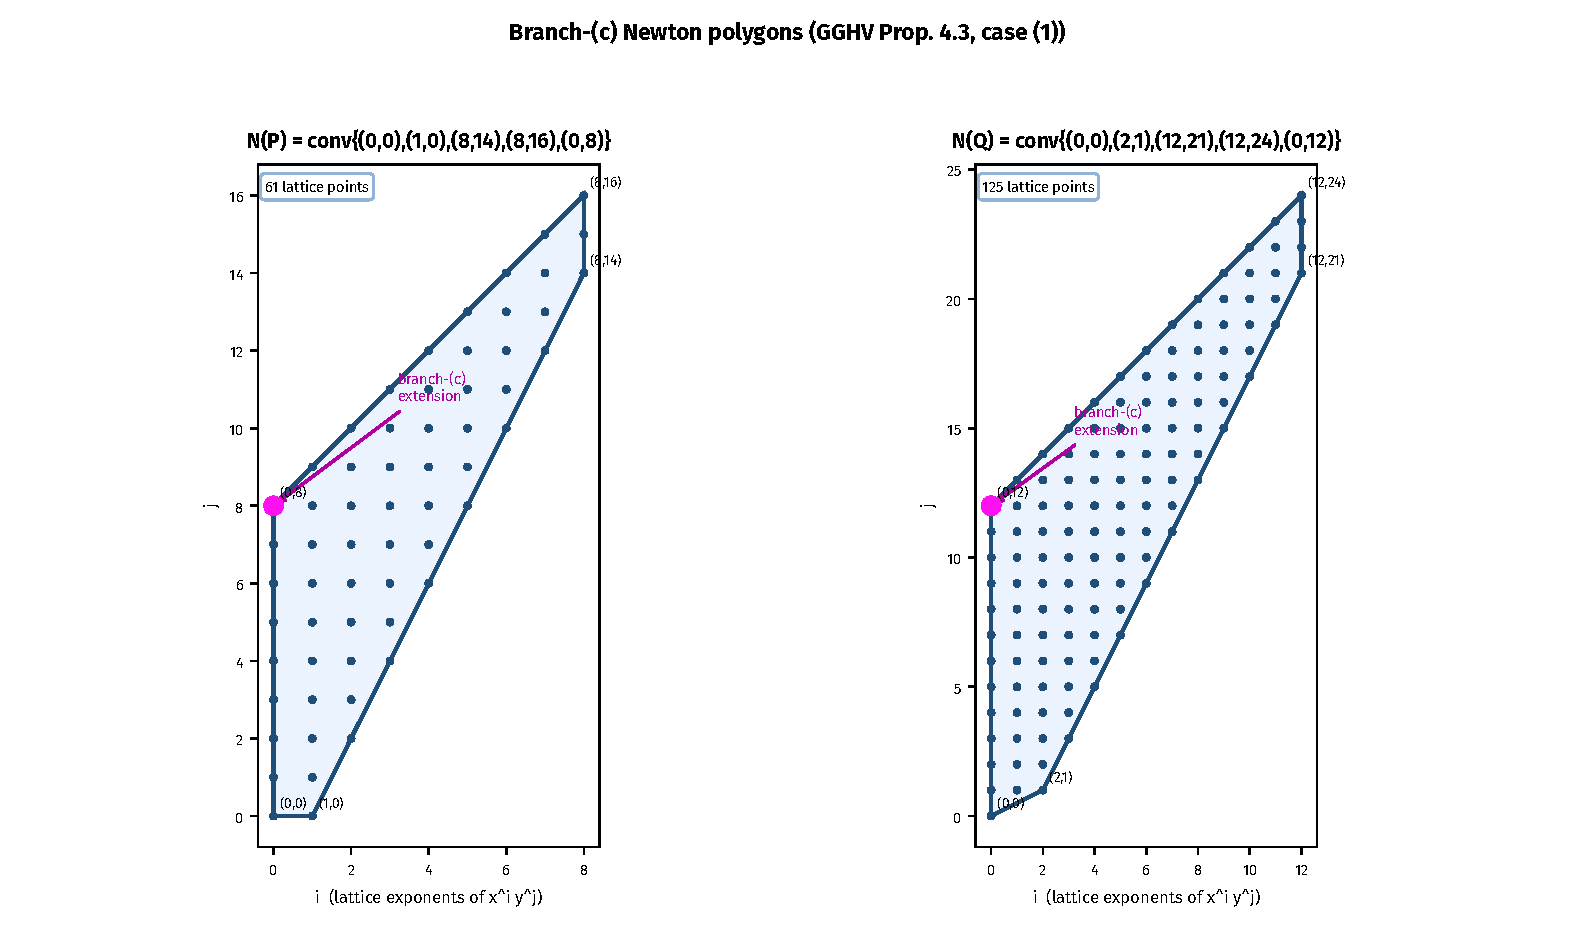
\includegraphics[width=0.95\textwidth]{figures_c/fig1_newton_polygons.pdf}
\caption{Branch-(c) Newton polygons, drawn from the exact vertex data of~\eqref{bc:eq:polygons}, which are checked against lines~494 and~617--618 of the text of~\cite{GGHV}, v1 (\S\ref{bc:sec:source}). In each panel the branch-(a,b) sub-polygon is drawn in the lighter shade underneath, and the extra branch-(c) vertices $(0,8)$ and $(0,12)$ are drawn in the accent colour. All lattice points are marked ($61$ for $N(P)$, $125$ for $N(Q)$), and the ten vertex coefficients that \texttt{NewtonNFc} requires to be nonzero are labelled. Drawn by \texttt{figures/fig1\_\allowbreak{}newton\_\allowbreak{}polygons.\allowbreak{}py} from the vertex lists.}
\label{bc:fig:polygons}
\end{figure}

Santib\'a\~nez-Leal has published machine evidence about the $(72,108)$ candidate~\cite{Santibanez,SantibanezPaper} and states explicitly that it does not amount to an elimination. The candidate itself is documented in~\cite{JC125note}. Two further treatments of the GGHV configuration appeared in 2026, neither peer-reviewed: Helali's exact characteristic-zero certificate~\cite{Helali} and the structural analysis of wstrinz~\cite{wstrinz}. The parity-constrained Davenport--Stothers equation that governs the top layer (\S\ref{bc:sec:top}) has not been classified in the literature.

\subsection{Main result}

We work over a field $L$ of characteristic~$0$ and write $L[x,y]$ for the polynomial ring in two variables.

\begin{definition}[Branch-(c) Newton normal form]\label{bc:def:newtonnfc}
Let $P,Q\in L[x,y]$. We say that $(P,Q)$ is in \emph{branch-(c) Newton normal form}, written \texttt{NewtonNFc}$(P,Q)$, when $\operatorname{supp}P\subset N(P)$ and $\operatorname{supp}Q\subset N(Q)$ for the polygons of~\eqref{bc:eq:polygons}, and the ten coefficients of $P$ at $(0,0)$, $(1,0)$, $(8,14)$, $(8,16)$, $(0,8)$ and of $Q$ at $(0,0)$, $(2,1)$, $(12,21)$, $(12,24)$, $(0,12)$ are all nonzero. The Lean definition is \texttt{NewtonNFc} in \filename{Jacobian/BranchC/DescentClaim.lean}, reproduced in Listing~\ref{bc:lst:newtonnfc}.
\end{definition}

Two facts about the proof assistant are used throughout. A Lean statement is \emph{kernel-checked} when the small trusted core of Lean~4 (the \emph{kernel}) has type-checked a proof term for it; everything else in the system, tactics included, only produces such terms. The command \texttt{\#print axioms} lists the axioms on which a kernel-checked theorem depends. The three axioms \texttt{propext}, \texttt{Classical.\allowbreak{}choice} and \texttt{Quot.\allowbreak{}sound} are the standard foundation of Lean's mathematical library, and a theorem whose list contains nothing else uses no added axiom and no unproved placeholder (\texttt{sorry}).

The proof reduces the problem, through a chain of exact steps, to a finite system of twelve polynomial equations in seven unknowns over the quintic number field $K_5$ of~\eqref{bc:eq:K5}. We call the set of their solutions with $b_{12,22}=1$ the \emph{chart} (\S\ref{bc:sec:conditions}), and we split it into two \emph{strata} according to whether the coefficient $b_{11,20}$ vanishes. The first form of the main theorem leaves the stratum $b_{11,20}\neq0$ as an explicit hypothesis.

\begin{theorem}[Elimination of the branch-(c) normal form, conditional form]\label{bc:thm:main}
Let $L$ be a field of characteristic~$0$ for which \texttt{ChartEmptyC\_\allowbreak{}T1ne0} holds (Listing~\ref{bc:lst:chartempty}), that is, the twelve chart conditions of \S\ref{bc:sec:conditions} have no common zero with $b_{12,22}=1$ and $b_{11,20}\neq0$. Then there are no $P,Q\in L[x,y]$ and no $\lambda\neq0$ with \texttt{NewtonNFc}$(P,Q)$ and $[P,Q]=\lambda x^2$.
\end{theorem}

The hypothesis \texttt{ChartEmptyC\_\allowbreak{}T1ne0} is a precise Lean proposition. It was first established outside Lean, by the rank lemma of \S\ref{bc:sec:wholechart}, at grade~B. Since November~4, 2026 it is a theorem of Lean with no hypotheses, \texttt{challenge\_\allowbreak{}target}, and this removes the hypothesis from Theorem~\ref{bc:thm:main}.

\begin{theorem}[Unconditional elimination of branch~(c) in Lean]\label{bc:thm:unconditional}
Let $L$ be a field of characteristic~$0$. There are no $P,Q\in L[x,y]$ and no $\lambda\neq0$ with \texttt{NewtonNFc}$(P,Q)$ and $[P,Q]=\lambda x^2$.
\end{theorem}

\begin{leanlisting}{\texttt{branch\_c\_eliminated}: unconditional branch-(c) elimination}{bc:lst:unconditional}
-- branch_c/grade_a/lean/GradeA/Composition.lean, lines 19-22 (verbatim)
theorem branch_c_eliminated {L : Type*} [Field L] [CharZero L] :
    ¬ ∃ (P Q : MvPolynomial (Fin 2) L) (lam : L), lam ≠ 0 ∧ NewtonNFc P Q ∧
      jac P Q = C lam * X 0 ^ 2 :=
  BranchC.main_theorem_c_of_chartEmpty_T1ne0 challenge_target
\end{leanlisting}

\begin{corollary}[The chart statement, unconditionally]\label{bc:cor:unconditional}
For every field $L$ of characteristic~$0$, \texttt{ChartEmptyC\_\allowbreak{}T1ne0} holds (\texttt{challenge\_\allowbreak{}target}), and so does the statement \texttt{ChartEmptyC} for the whole chart. The rank route of \S\ref{bc:sec:wholechart}, in which Lemma~\ref{bc:lem:rank} is applied at two primes by two independent implementations and checked against negative controls, gives the same conclusion independently, at grade~B.
\end{corollary}

\begin{corollary}[Application to the Jacobian conjecture]\label{bc:cor:gghv}
Assume that \cite[Prop.~4.3]{GGHV} is correct and that its list of cases is exhaustive. Then no counterexample to the planar Jacobian conjecture with degree pair $(72,108)$ arises from branch~(c).
\end{corollary}

\begin{proof}[Proof of Theorem~\ref{bc:thm:unconditional}, and its kernel record]
In Lean, the conditional form of the main result, Theorem~\ref{bc:thm:main}, is the theorem \texttt{main\_\allowbreak{}theorem\_\allowbreak{}c\_\allowbreak{}of\_\allowbreak{}\allowbreak chartEmpty\_\allowbreak{}T1ne0}. Applying it to \texttt{challenge\_\allowbreak{}target} gives \texttt{branch\_\allowbreak{}c\_\allowbreak{}eliminated}, which is the statement of Theorem~\ref{bc:thm:unconditional}. The proof of \texttt{challenge\_\allowbreak{}target} is explained in \S\ref{bc:sec:leanrank}: it is the rank argument of \S\ref{bc:sec:wholechart} carried out inside Lean at the prime $p=32003$. For both theorems \texttt{\#print axioms} returns exactly \texttt{propext}, \texttt{Classical.\allowbreak{}choice} and \texttt{Quot.\allowbreak{}sound}. This was recorded on November~4, 2026 on the build machine (logs \filename{bridge\_challenge\_target\_2026-11-04.log} and \filename{branch\_c\_eliminated\_2026-11-04.log}). The two theorems were first proved in scratch files and were filed on November~6, 2026 as the tracked modules \texttt{GradeA.\allowbreak{}Bridge} and \texttt{GradeA.\allowbreak{}Composition} (\filename{branch\_c/grade\_a/lean/GradeA/Bridge.lean} and \filename{branch\_c/grade\_a/lean/GradeA/Composition.lean}), where they were rebuilt under Lean~4.34.0 with the same three axioms.
\end{proof}

The scope of Theorem~\ref{bc:thm:unconditional} needs to be stated plainly. It disposes of one case, case~(1), of one proposition of~\cite{GGHV}. It does not by itself exclude the degree pair $(72,108)$, and it does not prove the planar Jacobian conjecture. Both of those would require in addition that \cite[Prop.~4.3]{GGHV} be correct and exhaustive, and that the reduction from the conjecture to that proposition be sound. We record that reduction as a premise and do not re-derive it.

\subsection{Logical status}

\begin{remark}\label{bc:rem:conditional}
Theorem~\ref{bc:thm:main} does not depend on~\cite{GGHV}. Its Lean proof starts from \texttt{NewtonNFc}$(P,Q)$ and $[P,Q]=\lambda x^2$ and reaches the chart statement through the descent, entirely inside Lean. The Lean theorem \texttt{main\_\allowbreak{}theorem\_\allowbreak{}c\_\allowbreak{}of\_\allowbreak{}\allowbreak chartEmpty\_\allowbreak{}T1ne0} (Listing~\ref{bc:lst:main}) derives the conclusion from the explicit hypothesis \texttt{ChartEmptyC\_\allowbreak{}T1ne0} (Listing~\ref{bc:lst:chartempty}); \texttt{\#print axioms} reports only the three standard axioms, and no \texttt{sorry}, added \texttt{axiom} or \texttt{native\_\allowbreak{}decide} occurs in the $790$ modules of the build. In terms of the steps B0--B7 of Table~\ref{bc:tab:bridges}, the chain is
\begin{align*}
&\texttt{NewtonNFc}+[P,Q]=\lambda x^2
\xrightarrow{\ \text{B0--B3}\ }\text{hypotheses of }\texttt{DescentClaimC}
\xrightarrow{\ \text{B4--B5}\ }\texttt{ChartEmptyC}\\
&\qquad\xrightarrow{\ \text{B6--B7}\ }\texttt{ChartEmptyC\_\allowbreak{}T1ne0}
\Longrightarrow\text{contradiction},
\end{align*}
where each arrow means that the target statement suffices to refute the source data. The theorem \texttt{challenge\_\allowbreak{}target} discharges \texttt{ChartEmptyC\_\allowbreak{}T1ne0} with no hypotheses, so the chain closes inside Lean. Only Corollary~\ref{bc:cor:gghv} uses \cite[Prop.~4.3]{GGHV}.
\end{remark}

\begin{remark}[A retraction]\label{bc:rem:retraction}
A preliminary version of this work used a ``reduction lemma'' asserting that an ideal which is the unit ideal modulo a prime $p$ is also the unit ideal over $\mathbb{Q}$. The statement is false. Take the single polynomial $F=1+109X$. Modulo~$109$ it reduces to the constant $1$, so it generates the unit ideal of $\mathbb{F}_{109}[X]$. Over $\mathbb{Q}$ it vanishes at $X=-1/109$, so it generates a proper ideal of $\mathbb{Q}[X]$. A Lean file that derives \texttt{False} from the lemma stated as an axiom is kept for the record, and every theorem that depended on the lemma is vacuous. The replacement is the rank lemma (Lemma~\ref{bc:lem:rank}). What lifts from $\mathbb{F}_p$ to characteristic~$0$ is full row rank of a Macaulay matrix of fixed degree, because full row rank is witnessed by a nonzero minor and the nonvanishing of a determinant survives the lift. Consistency of a system modulo~$p$ does not lift. Section~\ref{bc:sec:epistemic} returns to the distinction.
\end{remark}

\subsection{Outline}

Section~\ref{bc:sec:source} checks the input data against the text of~\cite{GGHV}. Section~\ref{bc:sec:system} sets up the coefficients and the grading, and Section~\ref{bc:sec:layers} derives the layer identities and the $132$ scalar equations from them. Section~\ref{bc:sec:normalization} uses the symmetries of the problem to reach the chart, and Section~\ref{bc:sec:top} recalls the top layer, which branch~(c) shares with branches~(a) and~(b). Section~\ref{bc:sec:descent} carries out the descent to twelve conditions by kernel reflection. Section~\ref{bc:sec:conditions} studies those conditions, Section~\ref{bc:sec:t1zero} eliminates the stratum $b_{11,20}=0$ inside Lean, and Section~\ref{bc:sec:wholechart} eliminates the whole chart by the rank lemma, first outside Lean and then inside it. Section~\ref{bc:sec:proof} assembles the proof, Section~\ref{bc:sec:epistemic} records the grade of each claim and what is not claimed, Section~\ref{bc:sec:modules} lists the Lean modules, and Sections~\ref{bc:sec:conclusion} and~\ref{bc:sec:attribution} conclude and give attribution. Figure~\ref{bc:fig:bridges} shows how the steps fit together.

\begin{figure}[htbp]
\centering
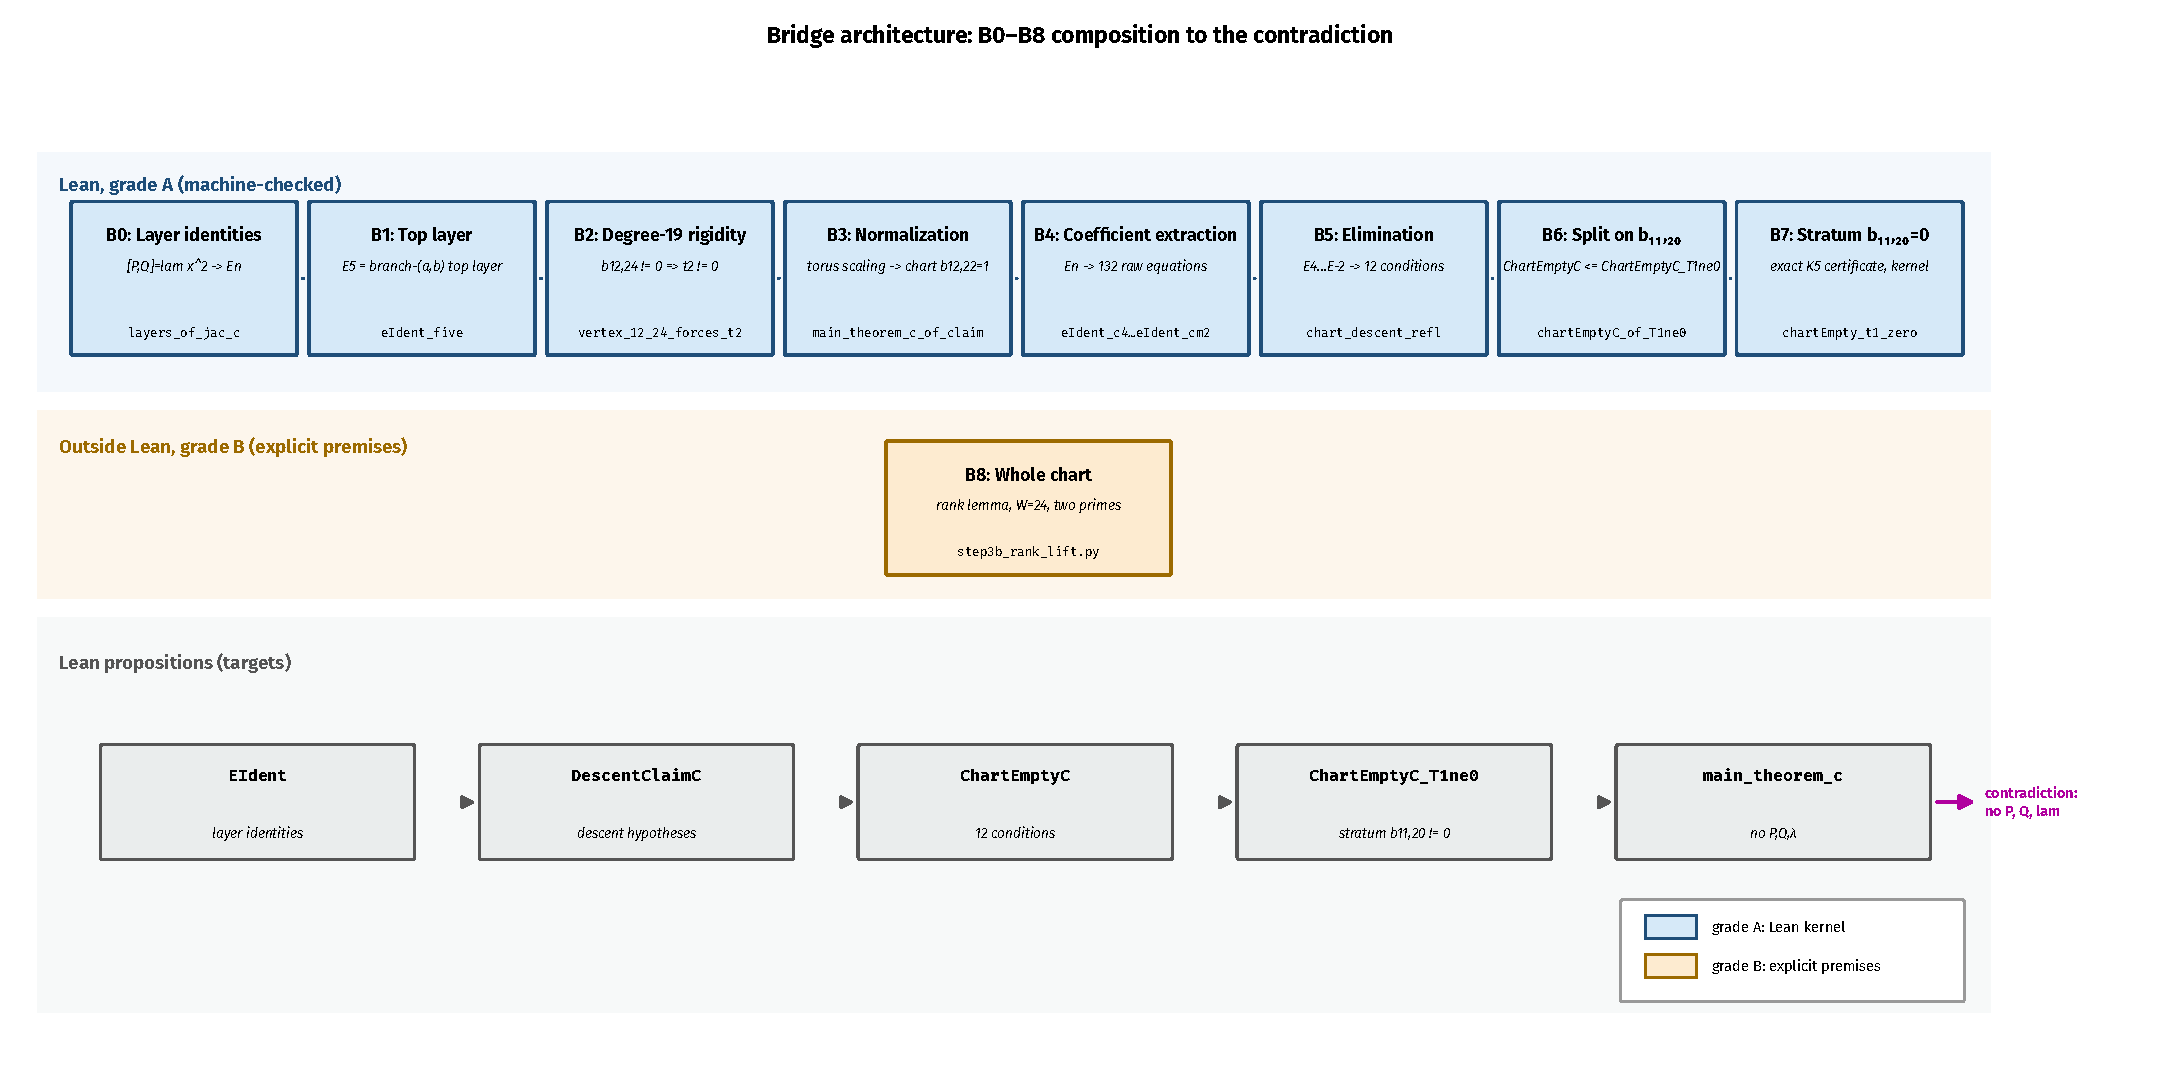
\includegraphics[width=0.97\textwidth]{figures_c/fig2_bridges.pdf}
\caption{How the steps compose. Top band: the eight Lean steps B0--B7 (grade~A), each labelled with its Lean name. Middle band: the rank lemma B8 (grade~B), now an independent corroboration of the Lean certificate of Theorem~\ref{bc:thm:unconditional}. Bottom band: the Lean propositions they reach, composing from left to right to the final contradiction. Colours follow the grades of Table~\ref{bc:tab:bridges}. Drawn by \texttt{figures/fig2\_\allowbreak{}bridges.\allowbreak{}py}.}
\label{bc:fig:bridges}
\end{figure}

\section{Source data}\label{bc:sec:source}

Every base object below was checked against the text of~\cite{GGHV}, v1, before any proof was written, as in Part~I (\S\ref{ab:sec:source}). The polygons~\eqref{bc:eq:polygons} are \cite[Prop.~4.3, case~(1)]{GGHV}. In the v1 text the vertex lists of case~(1) appear at line~494, and the list after the morphism $\varphi$ (called case~c there) at lines~617--618. The script \filename{source\_gate\_verify\_c.py} compares both lists byte for byte with the downloaded v1 text. The target $[P,Q]=\lambda x^2$ after $\varphi$ is taken from \cite[\S5]{GGHV}.

\begin{leanlisting}{The branch-(c) Newton normal form \texttt{NewtonNFc}}{bc:lst:newtonnfc}
-- Jacobian/BranchC/DescentClaim.lean (statement verbatim)
def NewtonNFc (P Q : MvPolynomial (Fin 2) K) : Prop :=
  (∀ m ∈ P.support, inNPc m) ∧ (∀ m ∈ Q.support, inNQc m) ∧
  P.coeff (mono 0 0) ≠ 0 ∧ P.coeff (mono 1 0) ≠ 0 ∧ P.coeff (mono 8 14) ≠ 0 ∧
  P.coeff (mono 8 16) ≠ 0 ∧ P.coeff (mono 0 8) ≠ 0 ∧
  Q.coeff (mono 0 0) ≠ 0 ∧ Q.coeff (mono 2 1) ≠ 0 ∧ Q.coeff (mono 12 21) ≠ 0 ∧
  Q.coeff (mono 12 24) ≠ 0 ∧ Q.coeff (mono 0 12) ≠ 0
-- inNPc, inNQc: the half-plane descriptions of the two polygons
\end{leanlisting}

The Lean development works over an arbitrary field of characteristic~$0$. The number field
\begin{equation}\label{bc:eq:K5}
K_5=\mathbb{Q}[w]/(R),\qquad R(w)=w^5-w^4+3w^3+3w^2+26,
\end{equation}
already used in Part~I (\S\ref{ab:sec:lifting}), enters through the top layer (\S\ref{bc:sec:top}). The polynomial $R$ is irreducible over $\mathbb{Q}$, so $K_5$ is a field of degree~$5$ over $\mathbb{Q}$. It stays irreducible modulo~$109$, so $\mathbb{F}_{109}[w]/(R)$ is the field $\mathbb{F}_{109^5}$; we call $109$ an \emph{inert} prime. A prime $p$ together with an integer $w_0$ satisfying $R(w_0)\equiv0\pmod p$ gives a ring homomorphism from the $p$-integral part of $K_5$ onto $\mathbb{F}_p$, sending $w$ to $w_0$. The pairs $(p,w_0)$ used below are
\begin{equation}\label{bc:eq:primes}
(101,9),\qquad (1000003,806739),\qquad (32003,11147).
\end{equation}
We checked the irreducibility of $R$ over $\mathbb{Q}$ and modulo $109$ and $67$, and the three congruences $R(w_0)\equiv0\pmod p$, with SymPy (script \filename{c2\_k5\_chart\_macaulay.py}, exit code~$0$).

\section{The polynomial system}\label{bc:sec:system}

\subsection{Lattice points}

Write $P=\sum a_{i,j}x^iy^j$ and $Q=\sum b_{i,j}x^iy^j$, where $(i,j)$ runs over the lattice points of $N(P)$ and of $N(Q)$ respectively. By Pick's theorem a lattice polygon of area $A$ with $B$ lattice points on its boundary has $I=A-B/2+1$ interior lattice points. For $N(P)$ we find $A=47$ and $B=26$, so $I=35$ and $|N(P)\cap\mathbb{Z}^2|=35+26=61$. For $N(Q)$ we find $A=105$ and $B=38$, so $I=87$ and $|N(Q)\cap\mathbb{Z}^2|=87+38=125$. Both counts agree with a direct enumeration. These supports strictly contain those of branches~(a) and~(b) (Part~I, \S\ref{ab:sec:system}), because of the vertices $(0,8)$ and $(0,12)$. In Lean the supports are encoded by the predicates \texttt{inNPc} and \texttt{inNQc}, and their layer-by-layer form by \texttt{rangeP} and \texttt{rangeQ} (\filename{Jacobian/BranchC/DescentClaim.lean}).

\subsection{The grading and the layers}

Give $x$ the weight $2$ and $y$ the weight $-1$, so that the monomial $x^iy^j$ has weight $2i-j$. Put $u=xy^2$, which has weight~$0$. Since $x^iy^j=u^i\,y^{j-2i}$, the part of $P$ of weight $k$ is $y^{-k}$ times a polynomial in $u$:
\begin{equation}\label{bc:eq:layers}
P=\sum_k y^{-k}A_k(u),\qquad Q=\sum_l y^{-l}B_l(u),\qquad A_k=\sum_{2i-j=k}a_{i,j}u^i,\quad B_l=\sum_{2i-j=l}b_{i,j}u^i .
\end{equation}
This is the decomposition~\eqref{ab:eq:decomp} of Part~I. We call $A_k$ the \emph{layer} of $P$ of index $k$ and $B_l$ the layer of $Q$ of index $l$. On the polygons~\eqref{bc:eq:polygons} the index $k=2i-j$ runs from $-8$ (at the vertex $(0,8)$) to $2$ (on the edge from $(1,0)$ to $(8,14)$), and $l$ runs from $-12$ (at $(0,12)$) to $3$ (on the edge from $(2,1)$ to $(12,21)$).

The bracket of two layers is again a single layer. Let $A,B\in L[u]$ and put $f=y^{-k}A(xy^2)$, $g=y^{-l}B(xy^2)$. Differentiating,
\[
f_x=y^{2-k}A',\qquad f_y=-k\,y^{-k-1}A+2u\,y^{-k-1}A',
\]
and similarly for $g$, where $A'$ and $B'$ are evaluated at $u$. Hence
\begin{align*}
[f,g]&=y^{2-k}A'\bigl(-l\,y^{-l-1}B+2u\,y^{-l-1}B'\bigr)-\bigl(-k\,y^{-k-1}A+2u\,y^{-k-1}A'\bigr)y^{2-l}B'\\
&=y^{1-k-l}\bigl(-lA'B+2uA'B'+kAB'-2uA'B'\bigr)\\
&=y^{1-k-l}\,\mathrm{LT}_{k,l}(A,B),\qquad \mathrm{LT}_{k,l}(A,B):=kAB'-lA'B .
\end{align*}
The right-hand side of the bracket condition is $\lambda x^2=\lambda u^2y^{-4}$, which is the power $y^{1-n}$ with $n=5$. Collecting the bracket of~\eqref{bc:eq:layers} by powers of $y$ and comparing with $\lambda u^2y^{-4}$ therefore splits $[P,Q]=\lambda x^2$ into one polynomial identity in $u$ for each $n=k+l$:
\begin{equation}\label{bc:eq:eident}
\texttt{EIdent}\ A\ B\ \lambda\ n:\qquad \sum_{k+l=n}\mathrm{LT}_{k,l}(A_k,B_l)=[n=5]\,\lambda u^2,
\end{equation}
where $[n=5]$ is $1$ if $n=5$ and $0$ otherwise. We write $E_n$ for this identity. The top identity $E_5$ involves only $k=2$ and $l=3$ and carries the term $\lambda u^2$; all the others are homogeneous.

Each identity $E_n$ is a list of scalar equations, one for each power of $u$. If $A_k$ contributes $a\,u^{i_1}$ and $B_l$ contributes $b\,u^{i_2}$, then $kAB'$ contributes $k\,i_2\,ab\,u^{i_1+i_2-1}$ and $lA'B$ contributes $l\,i_1\,ab\,u^{i_1+i_2-1}$. So the coefficient of $ab$ in the equation for $u^m$ is
\[
c=k\,(m+1-i_1)-l\,i_1,\qquad l=n-k,\quad i_2=m+1-i_1 .
\]
A coefficient $u^m$ of the layer $n$ corresponds to the monomial $u^my^{1-n}=x^my^{2m+1-n}$ of $[P,Q]$, so the scalar equation for the monomial $x^iy^j$ sits in layer $n=2i+1-j$ at the power $m=i$. These bookkeeping identities, the lattice counts, and the equation counts below were all checked with SymPy (script \filename{c1\_layers.py}, exit code~$0$).

\section{Exact layer reduction}\label{bc:sec:layers}

The layer indices satisfy $-8\le k\le2$ and $-12\le l\le3$, so $n=k+l$ lies between $-20$ and $5$. At $n=-20$ the only term is $\mathrm{LT}_{-8,-12}(A_{-8},B_{-12})$, and both $A_{-8}=a_{0,8}$ and $B_{-12}=b_{0,12}$ are constants, so this term vanishes identically. The lowest layer that carries an equation is $n=-19$.

\emph{Step B0} (Lean). From $\texttt{jac}(P,Q)=C\,\lambda\cdot x^2$ and \texttt{NewtonNFc}$(P,Q)$, the identities $\texttt{EIdent}\ A\ B\ \lambda\ n$ hold for every $n\ge-20$. This is \texttt{layers\_\allowbreak{}of\_\allowbreak{}jac\_\allowbreak{}c} (\filename{Jacobian/BranchC/LayersGen.lean}, line~131), proved from the general bracket formula \texttt{layer\_\allowbreak{}bracket\_\allowbreak{}gen} of the same file; the identity \eqref{bc:eq:eident} itself is the definition \texttt{EIdent} there. The step is an exact symbolic identity checked by the Lean kernel.

The descent uses the seven layers $n=4,3,\dots,-2$. Counting the powers of $u$ that can occur in $\sum_{k+l=n}\mathrm{LT}_{k,l}(A_k,B_l)$ with nonzero coefficient, for supports in~\eqref{bc:eq:polygons}, gives
\begin{center}
\begin{tabular}{lcccccccc}
\toprule
layer $n$ & $5$ & $4$ & $3$ & $2$ & $1$ & $0$ & $-1$ & $-2$\\
scalar equations & $17$ & $18$ & $19$ & $19$ & $20$ & $19$ & $19$ & $18$\\
\bottomrule
\end{tabular}
\end{center}
so the layers $n=4,\dots,-2$ contribute $18+19+19+20+19+19+18=132$ scalar equations. The top layer $n=5$ has $17$ equations, as in branches~(a) and~(b) (Part~I, Proposition~\ref{ab:prop:layers}). The $132$ equations involve $142$ coefficients: the $8+11=19$ coefficients of the top layers $A_2$ (the $a_{i,2i-2}$, $1\le i\le8$) and $B_3$ (the $b_{i,2i-3}$, $2\le i\le12$), and $123$ further coefficients, which we call the \emph{unknowns}.

\emph{Step B4} (Lean). Coefficient extraction turns the polynomial identities $\texttt{EIdent}\ A\ B\ 0\ n$, $n=4,\dots,-2$, into these $132$ scalar equations. For each monomial of $\mathrm{LT}_{k,l}(A_k,B_l)$ the lemma \texttt{coeff\_\allowbreak{}layerTermZ} computes its coefficient with integer indices, by the formula for $c$ above. Coefficients outside the supports vanish by \texttt{rangeP} and \texttt{rangeQ}; this produces $179$ vanishing facts. The coefficients $a_{0,0}$ and $b_{0,0}$ lie in the supports but never occur, since constants have zero derivative. Each of the $132$ equations then follows by \texttt{linear\_\allowbreak{}combination}. The lemmas are \texttt{eIdent\_\allowbreak{}c4}, \texttt{eIdent\_\allowbreak{}c3}, \texttt{eIdent\_\allowbreak{}c2c}, \texttt{eIdent\_\allowbreak{}c1}, \texttt{eIdent\_\allowbreak{}c0}, \texttt{eIdent\_\allowbreak{}cm1} and \texttt{eIdent\_\allowbreak{}cm2} in \filename{Jacobian/BranchC/Descent2R/Bridge.lean}, which is generated by \filename{certgen\_c/gen\_bridge\_c.py} following the recipe of the branch-(a,b) file \filename{BranchAbFinal.lean}.

\section{Normalization}\label{bc:sec:normalization}

\emph{Step B1} (Lean). The top identity $E_5$ involves only $A_2$ and $B_3$, and it is the same identity as in branches~(a) and~(b), because the vertices $(0,8)$ and $(0,12)$ do not touch the top layers. Part~I classifies its solutions exactly over $K_5$, in five torus orbits (Part~I, Proposition~\ref{ab:prop:top-class} and Theorem~\ref{ab:thm:chartclass}, the Lean theorem \texttt{chartClassification\_\allowbreak{}holds} in \filename{Jacobian/ChartProof/Final.lean}). Branch~(c) inherits this classification unchanged. This is where $w$ and $R$ enter. The Lean lemma that reads off $E_5$ in the form needed by the classification is \texttt{eIdent\_\allowbreak{}five} (\filename{Jacobian/BranchC/LayersGen.lean}, line~231).

\emph{Step B2} (Lean). The vertex $(12,24)$ of $N(Q)$ forces $t_2:=b_{12,22}\neq0$. We give the argument in full. Grade $L[x,y]$ by the degree in $x$ alone. For one-variable polynomials $f,g$ one has
\[
[x^if(y),\,x^kg(y)]=x^{i+k-1}\bigl(i\,fg'-k\,f'g\bigr),
\]
so the bracket of the parts of $x$-degree $i$ and $k$ has $x$-degree $i+k-1$. Since $P$ has $x$-degree at most $8$ and $Q$ at most $12$, the part of $[P,Q]$ of $x$-degree $19$ is the bracket of the columns $x^8f(y)$ and $x^{12}g(y)$ of $P$ and $Q$, where by~\eqref{bc:eq:polygons}
\[
f=\alpha y^{14}+a_1y^{15}+a_0y^{16},\qquad g=\beta y^{21}+t\,y^{22}+s\,y^{23}+b\,y^{24},
\]
with $\alpha=a_{8,14}$, $a_1=a_{8,15}$, $a_0=a_{8,16}$, $\beta=b_{12,21}$, $t=t_2=b_{12,22}$, $s=b_{12,23}$ and $b=b_{12,24}$. As $[P,Q]=\lambda x^2$ has no part of $x$-degree $19$, we get $8fg'-12f'g=0$. Expanding, the only powers of $y$ that occur are $y^{35},\dots,y^{38}$, with coefficients $4$ times
\begin{equation}\label{bc:eq:edge19}
2\alpha t-3\beta a_1,\qquad 4\alpha s-a_1t-6\beta a_0,\qquad 6\alpha b+a_1s-4a_0t,\qquad 3a_1b-2a_0s .
\end{equation}
Suppose $t=0$. The first expression gives $3\beta a_1=0$, and $\beta\neq0$ because $(12,21)$ is a vertex, so $a_1=0$. The third expression then reduces to $6\alpha b=0$, and $\alpha\neq0$ because $(8,14)$ is a vertex, so $b=b_{12,24}=0$, contradicting \texttt{NewtonNFc}. Hence $t_2\neq0$. Using all four expressions with $\alpha\neq0$ one obtains more: the identities
\[
\alpha\,(3\beta s-t^2)^2\in\bigl(\text{the four expressions}\bigr),\qquad 3\beta s=t^2,\qquad 27\beta^2b=t^3,
\]
the last one following from $\alpha(27\beta^2b-9\beta st+2t^3)$, which also lies in the ideal, together with $3\beta s=t^2$. They say that $f=\alpha(1+\gamma y)^2y^{14}$ and $g=\beta(1+\gamma y)^3y^{21}$ with $\gamma=t/(3\beta)$, and they give $b_{12,24}=t_2^3/(27b_{12,21}^2)$ directly. The expansion and the two ideal memberships, with the cofactors used in Lean, were checked with SymPy (script \filename{c4\_edge19.py}, exit code~$0$).

In Lean the four equations~\eqref{bc:eq:edge19} are \texttt{edge\_\allowbreak{}coeffs}, the relations $3\beta s=t^2$ and $27\beta^2b=t^3$ are \texttt{edge19\_\allowbreak{}rigidity} (line~324) and, read off from $P$ and $Q$, \texttt{edge19\_\allowbreak{}rigidity\_\allowbreak{}of\_\allowbreak{}jac} (line~412), and the conclusion $t_2\neq0$ is \texttt{vertex\_\allowbreak{}12\_\allowbreak{}24\_\allowbreak{}forces\_\allowbreak{}t2} (line~423), all in \filename{Jacobian/BranchC/Edge19.lean}. The special case $t_2=0\Rightarrow b_{12,24}=0$ is the \emph{degree-$19$ rigidity} lemma. In the narrower situation where both parameters $t_1,t_2$ of the kernel of $E_4$ vanish (Part~I, Corollary~\ref{ab:cor:t0}), there is a second proof through the layer identity $E_2$. Then the layers $A_1$ and $B_2$ vanish, and $E_2$ reduces to $2A_2B_0'=A_{-1}B_3'+3A_{-1}'B_3$. The coefficient of $u^{19}$ on the left is $2\cdot[u^8]A_2\cdot12\,[u^{12}]B_0=24\,a_{8,14}\,b_{12,24}$, while $\deg A_{-1}\le7$ bounds the right side by degree~$18$. This is \texttt{degree19\_\allowbreak{}rigidity} (\filename{Jacobian/BranchC/Degree19.lean}, line~125), and its application to $P$ and $Q$ is \texttt{t0\_\allowbreak{}vertex\_\allowbreak{}rigidity\_\allowbreak{}of\_\allowbreak{}jac} (\filename{Jacobian/BranchC/LayerE2.lean}, line~270). The degree count was checked in \filename{c3\_transport\_deg19.py} (exit code~$0$).

\emph{Step B3} (Lean). The torus and a weighted scaling remove the continuous symmetries. For constants $\alpha,\beta,\kappa,\tau$ with $\tau\neq0$, consider the substitution
\[
A_k(u)\longmapsto\alpha\,\tau^{2-k}A_k(\kappa u),\qquad B_l(u)\longmapsto\beta\,\tau^{3-l}B_l(\kappa u).
\]
Writing $\tilde A(u)=A(\kappa u)$ we have $\tilde A'(u)=\kappa A'(\kappa u)$, so
\[
\mathrm{LT}_{k,l}\bigl(\alpha\tau^{2-k}\tilde A_k,\ \beta\tau^{3-l}\tilde B_l\bigr)=\alpha\beta\,\tau^{5-k-l}\,\kappa\ \mathrm{LT}_{k,l}(A_k,B_l)(\kappa u).
\]
The factor $\alpha\beta\tau^{5-n}\kappa$ depends only on $n=k+l$, so every homogeneous identity $E_n$, $n\neq5$, is carried to an identity of the same form. This is \texttt{eIdent\_\allowbreak{}transport} (\filename{Jacobian/BranchC/DescentClaim.lean}, line~117); the identity was checked with SymPy in \filename{c3\_transport\_deg19.py} (exit code~$0$). The classification of Step~B1 provides $\alpha,\beta,\kappa$ that carry $(A_2,B_3)$ to the fixed $K_5$ solution, and since $t_2\neq0$ by Step~B2 the remaining freedom in $\tau$ can be spent to make the transported coefficient $[u^{12}]B_2=\beta\tau\kappa^{12}t_2$ equal to $1$. The result is the \emph{chart} normalization $b_{12,22}=1$. The theorem \texttt{main\_\allowbreak{}theorem\_\allowbreak{}c\_\allowbreak{}of\_\allowbreak{}claim} (\filename{Jacobian/BranchC/DescentClaim.lean}, line~149) carries this out. It shows that a branch-(c) pair produces data satisfying the hypotheses of the proposition \texttt{DescentClaimC} (line~90 of the same file): a root $w$ of $R$, the $19$ top-layer values given as explicit elements of $\mathbb{Q}(w)$, the $123$ unknowns, the layer identities for $-2\le n\le4$, and $b_{12,22}=1$. \texttt{DescentClaimC} asserts that such data do not exist.

\section{The top layer}\label{bc:sec:top}

At $n=5$ the layer equations of branch~(c) are those of the branch-(a,b) top layer, whose complete classification over $K_5$ is proved in Part~I (\S\ref{ab:sec:top}; Proposition~\ref{ab:prop:top-class}) and in~\cite{BranchABv19}: five torus orbits, with a degree-$35$ eliminant irreducible over $\mathbb{Q}$. After the substitution $u=s^2$ the identity $E_5$ becomes the Davenport--Stothers equation $2fg'-3f'g=c$ with $f$ even and $g$ odd~\cite{Davenport,Stothers} (Part~I, \eqref{ab:eq:e5}). We use the classification as a closed result. The $19$ top-layer values enter \filename{Jacobian/BranchC/Descent2R/Main.lean} as hypotheses, with $a_{1,0}=b_{2,1}=1$ and the others explicit elements of $\mathbb{Q}(w)$; for instance
\[
a_{2,2}=\tfrac{303}{16}+\tfrac{879}{128}w-\tfrac{389}{128}w^2-\tfrac{51}{128}w^3+\tfrac{49}{128}w^4 .
\]
The $K_5$ arithmetic they satisfy is exactly the arithmetic of~\eqref{bc:eq:K5}. Branch~(c) needs no new analysis of the top layer. What is new is the descent of \S\ref{bc:sec:descent} and the chart analysis of \S\S\ref{bc:sec:conditions}--\ref{bc:sec:wholechart}.

\paragraph{The degree-$19$ step is formalized.} An audit of the branch-(c) development dated September~26, 2026 identified the degree-$19$ rigidity lemma of Step~B2 as the one place below the chart where the argument left the Lean kernel: at that date the lemma was supplied by a certified point from an external file, checked in Lean by evaluation, with the classification argument itself graded~B. That gap has been closed. The lemma is now the Lean theorem \texttt{degree19\_\allowbreak{}rigidity} (\filename{Jacobian/BranchC/Degree19.lean}), and its use on a branch-(c) pair goes through \texttt{vertex\_\allowbreak{}12\_\allowbreak{}24\_\allowbreak{}forces\_\allowbreak{}t2} and \texttt{edge19\_\allowbreak{}rigidity\_\allowbreak{}of\_\allowbreak{}jac} (\filename{Jacobian/BranchC/Edge19.lean}). For all three, \texttt{\#print axioms} lists only \texttt{propext}, \texttt{Classical.\allowbreak{}choice} and \texttt{Quot.\allowbreak{}sound}. The theorem \texttt{main\_\allowbreak{}theorem\_\allowbreak{}c\_\allowbreak{}of\_\allowbreak{}claim} (\filename{Jacobian/BranchC/DescentClaim.lean}) calls \texttt{vertex\_\allowbreak{}12\_\allowbreak{}24\_\allowbreak{}forces\_\allowbreak{}t2} and the top-layer classification \texttt{chartClassification\_\allowbreak{}holds} directly, and it has the same three axioms. No branch-(c) Lean file reads an external certificate. The same audit noted that a line reference to~\cite{GGHV} was missing; \S\ref{bc:sec:attribution} supplies it. Closing this gap does not touch the hypotheses of Corollary~\ref{bc:cor:gghv}: the application to the degree pair $(72,108)$ remains conditional on \cite[Prop.~4.3]{GGHV}.

\section{Descent}\label{bc:sec:descent}

\emph{Step B5} (Lean, by kernel reflection). We solve the layers in the order $n=4,3,\dots,-2$. Once the top layer and the earlier layers are fixed, each identity $E_n$ is a linear system in the coefficients that appear in it for the first time, and its coefficients are polynomials in the earlier unknowns and the chart parameters. Exact ranks of these systems over $K_5$ are proved by the operator-rank theorems of the directory \filename{Jacobian/BranchC/Rank/} ($96$ modules). Wherever a system has a left null vector, that is, a linear combination of its equations in which all new unknowns cancel, the same combination of the right-hand sides must vanish, and this gives a condition on the earlier data. Table~\ref{bc:tab:descent} lists what each layer produces.

\begin{table}[htbp]
\centering
\small
\begin{tabular}{ll>{\raggedright\arraybackslash}p{0.5\textwidth}}
\toprule
Layer & Lean modules & Conditions produced \\
\midrule
$E_4$ ($n=4$) & \texttt{Descent2R/L4} ($54$) & none \\
$E_3$ ($n=3$) & \texttt{Descent2R/L3} ($57$) & none \\
$E_2$ ($n=2$) & \texttt{Descent2R/L2c} ($57$) & none (the left null vector annihilates the right-hand side) \\
$E_1$ ($n=1$) & \texttt{Descent2R/L1} ($60$) & $\Omega$ \\
$E_0$ ($n=0$) & \texttt{Descent2R/L0} ($60$) & $\Psi$ and the pure row \texttt{E0pure\_\allowbreak{}18\_\allowbreak{}37} \\
$E_{-1}$ ($n=-1$) & \texttt{Descent2R/Lm1} ($99$) & $\Phi_1,\Phi_2$ and the pure rows \texttt{Em1pure\_\allowbreak{}17\_\allowbreak{}36}, \texttt{Em1pure\_\allowbreak{}18\_\allowbreak{}38} \\
$E_{-2}$ ($n=-2$) & \texttt{Descent2R/Lm2} ($110$) & $\Theta_1,\Theta_2,\Theta_3$ and the pure rows \texttt{Em2pure\_\allowbreak{}16\_\allowbreak{}35}, \texttt{Em2pure\_\allowbreak{}17\_\allowbreak{}37} \\
\bottomrule
\end{tabular}
\caption{The conditions produced by the layers $E_4,\dots,E_{-2}$. A \emph{pure row} is a condition read off a single equation of the layer in which no new unknown occurs.}
\label{bc:tab:descent}
\end{table}

The eliminations were first computed in Python by the script \filename{lower\_c.py}. The directory \filename{Descent2R} replays them in Lean as $600$ polynomial identities of the form $\mathrm{target}=\sum_i m_i\cdot\mathrm{fact}_i$, where each $\mathrm{fact}_i$ is a raw equation or an earlier target and the $m_i$ are polynomial multipliers. Each identity is checked by the Lean kernel through \emph{reflection}: the two sides are written as terms of an expression datatype (\texttt{Expr}), a normalizing function written in Lean (\texttt{toPolyK}) turns each into a canonical polynomial, and the kernel evaluates that function and compares the results by \texttt{decide +kernel}. The library is the branch-(a,b) file \filename{Jacobian/ChartProof/Reflect.lean}, built on the commutative-ring normalizer \texttt{Lean.\allowbreak{}Grind.\allowbreak{}CommRing} of the Lean core. Each step theorem has the form $(\texttt{Expr.\allowbreak{}mul}\ (\texttt{.\allowbreak{}num}\ K)\ X)\texttt{.\allowbreak{}denote}\ \mathrm{ctx}=0$ and is proved by \texttt{lc\_\allowbreak{}zero} (\filename{Reflect.lean}, line~130) with one kernel \texttt{decide}. When the clearing integer $K$ is not $1$, the main file removes it by \texttt{cancel\_\allowbreak{}int}, using that $K\neq0$ in characteristic~$0$; this happens for $231$ of its $752$ intermediate steps. The evaluation context \texttt{gctx2} consists of $143$ atoms, namely $w$, the seven chart parameters, the $19$ top-layer values and the $123$ unknowns less the parameters already listed, stored in a balanced tree. A tactic proof of the same identities was tried first and abandoned, because the source reached $214$~MB and chunks took over $10$ minutes each. The kernel evaluates the normalizer directly with GMP arithmetic. The tactic \texttt{decide +kernel} is not \texttt{native\_\allowbreak{}decide}: no compiled code is trusted.

The main theorem of the descent is \texttt{chart\_\allowbreak{}descent\_\allowbreak{}refl} (\filename{Jacobian/BranchC/Descent2R/Main.lean}, line~530). Its hypotheses list $w$, the $19$ top-layer values with their explicit values, the unknowns and the $132$ raw equations one by one; Listing~\ref{bc:lst:descent} shows its shape.

\begin{leanlisting}{\texttt{chart\_descent\_refl}: the twelve conditions from the $132$ raw equations (abridged)}{bc:lst:descent}
-- Jacobian/BranchC/Descent2R/Main.lean (abridged: hypotheses grouped, 752 steps elided)
theorem chart_descent_refl {L : Type*} [Field L] [CharZero L]
    (w : L) (hw : w ^ 5 - w ^ 4 + 3 * w ^ 3 + 3 * w ^ 2 + 26 = 0)
    (a_1_0 ... b_12_21 : L)                          -- the 19 top-layer values
    (h_a_1_0 : a_1_0 = 1) ... (h_b_12_21 : b_12_21 = ...)
    (b_11_20 ... : L)                                -- the 123 unknowns
    (h4_... : ...) ... (hm2_17_37 : ...) :           -- the 132 raw equations
    cond_Omega w ... = 0 ∧ cond_Psi w ... = 0 ∧
    cond_Phi1 w ... = 0 ∧ cond_Phi2 w ... = 0 ∧
    cond_Theta1 w ... = 0 ∧ cond_Theta2 w ... = 0 ∧ cond_Theta3 w ... = 0 ∧
    cond_E0pure_18_37 w ... = 0 ∧ cond_Em1pure_17_36 w ... = 0 ∧
    cond_Em1pure_18_38 w ... = 0 ∧ cond_Em2pure_16_35 w ... = 0 ∧
    cond_Em2pure_17_37 w ... = 0
\end{leanlisting}

The twelve conjuncts are the conditions of \filename{lower\_c.py}, each multiplied by an explicit positive integer. They are defined once, in \filename{Jacobian/BranchC/CondsC.lean}, which is generated by \filename{certgen\_c/gen\_conds\_c.py}. Each \texttt{cond\_\allowbreak{}*} is written as an explicit polynomial with the same balanced sum tree as the reflected fact, subtrees of at most $32$ terms being separate definitions ($110$ definitions for the $12$ conditions). Consequently the statement that the reflected term evaluates to $0$ and the statement \texttt{cond\_\allowbreak{}*}~$\dots=0$ are equal by definition, and no further proof is needed to pass from one to the other. The file \filename{Jacobian/BranchC/Descent2R/Bridge.lean} then proves \texttt{descentClaimC\_\allowbreak{}of\_\allowbreak{}\allowbreak chartEmpty} (line~166): the statement \texttt{ChartEmptyC} (line~149), that the twelve conditions have no common zero on the chart, implies \texttt{DescentClaimC}.

\section{The chart conditions}\label{bc:sec:conditions}

\subsection{Chart variables}

After the normalization $b_{12,22}=1$, the twelve conditions are polynomials in $w$ and seven coefficients, which we rename as follows. Each name carries a weight, and with these weights every condition is weighted homogeneous before the normalization $T_2=1$.

\begin{center}
\begin{tabular}{lccccccc}
\toprule
Symbol & $T_1$ & $T_2$ & $S_1$ & $S_2$ & $R_1$ & $R_2$ & $Q$ \\
Coefficient & $b_{11,20}$ & $b_{12,22}$ & $b_{11,21}$ & $b_{12,23}$ & $a_{6,13}$ & $a_{7,15}$ & $b_{10,21}$ \\
Weight & $1$ & $1$ & $2$ & $2$ & $3$ & $3$ & $4$ \\
\bottomrule
\end{tabular}
\end{center}

The \emph{chart} is the set of points $(T_1,S_1,S_2,R_1,R_2,Q)$ with $T_2=1$ at which all twelve conditions vanish, for a root $w$ of $R$ in $L$. The stratum $b_{11,20}=0$ is the part of the chart with $T_1=0$, and the stratum $b_{11,20}\neq0$ is its complement.

\subsection{The twelve conditions}\label{bc:sec:twelve}

The conditions are stored in the file \filename{certgen\_c/conds\_c.json}, written by \filename{certgen\_c/lower\_c.py}; its MD5 checksum is\linebreak[0] \texttt{168299d255af3615}\allowbreak\texttt{78423c0ed4852c11}. Table~\ref{bc:tab:conds} gives, for each, its weighted degree, the number of its terms as a polynomial with coefficients in $K_5$, and the number of its terms once it is scaled to integer coefficients and $w$ is treated as a further variable.

\begin{table}[htbp]
\centering
\begin{tabular}{lccc}
\toprule
Condition & weight & $K_5$-terms & integer terms \\
\midrule
$\Omega$ & $4$ & $3$ & $15$ \\
$\Psi$ & $5$ & $32$ & $160$ \\
$\Phi_1,\ \Phi_2$ & $6$ & $54,\ 54$ & $270,\ 270$ \\
$\Theta_1,\ \Theta_2,\ \Theta_3$ & $7$ & $84,\ 84,\ 84$ & $420,\ 420,\ 420$ \\
\texttt{E0pure\_\allowbreak{}18\_\allowbreak{}37} & $5$ & $9$ & $41$ \\
\texttt{Em1pure\_\allowbreak{}17\_\allowbreak{}36}, \texttt{Em1pure\_\allowbreak{}18\_\allowbreak{}38} & $6$ & $39,\ 12$ & $195,\ 60$ \\
\texttt{Em2pure\_\allowbreak{}16\_\allowbreak{}35}, \texttt{Em2pure\_\allowbreak{}17\_\allowbreak{}37} & $7$ & $77,\ 55$ & $381,\ 275$ \\
\bottomrule
\end{tabular}
\caption{The twelve chart conditions. Term counts and weights were recomputed from \texttt{conds\_\allowbreak{}c.\allowbreak{}json} with SymPy (\texttt{c2\_\allowbreak{}k5\_\allowbreak{}chart\_\allowbreak{}macaulay.\allowbreak{}py}, exit code~$0$).}
\label{bc:tab:conds}
\end{table}

\subsection{\texorpdfstring{The $\Omega$ parabola}{The Omega parabola}}\label{bc:sec:omega}

The condition of lowest weight has only three terms. Exactly over $K_5$,
\begin{equation}\label{bc:eq:omega}
\Omega=o_1S_2^2+o_2T_2^2S_2+o_3T_2^4,\qquad o_2^2=4o_1o_3,\qquad o_1\neq0 .
\end{equation}
A binary quadratic form with vanishing discriminant is a constant multiple of a square. Explicitly, put $\kappa=-o_2/(2o_1)\in K_5$. Then $o_2=-2o_1\kappa$ and $o_3=o_2^2/(4o_1)=o_1\kappa^2$, so
\begin{equation}\label{bc:eq:omegafactor}
\Omega=o_1\bigl(S_2^2-2\kappa T_2^2S_2+\kappa^2T_2^4\bigr)=o_1\bigl(S_2-\kappa T_2^2\bigr)^2 .
\end{equation}
The relation $o_2^2=4o_1o_3$ was checked by the scripts \filename{step1/lowerc\_chart.py} and \filename{step3c\_chart\_identity.py}, and again here (\filename{c2\_k5\_chart\_macaulay.py}). The inequality $o_1(w)\neq0$ is proved in the Lean kernel by a Bezout identity $a\cdot N_{o_1}+b\cdot R=c$, where $N_{o_1}$ is the integer polynomial representing $o_1$ and $c$ is a nonzero integer of $151$ digits (\texttt{T1Zero.\allowbreak{}s\_\allowbreak{}X2}). On the chart $T_2=1$ the equation $\Omega=0$ therefore forces $S_2=\kappa$. The common denominator of $\kappa$ is $D_k=851565312$, and $D_k^2\Omega=o_1\,(D_kS_2-D_k\kappa)^2$ at $T_2=1$ (Figure~\ref{bc:fig:omega}). The same double root appears at Step~B2: in the coordinates $t_2,s_2$ the relation $3\beta s=t^2$ obtained there from~\eqref{bc:eq:edge19} is the obstruction $\Omega=0$, with double root $\kappa=1/(3b_{12,21})$ (\filename{Jacobian/BranchC/OmegaEdge.lean}).

\begin{figure}[htbp]
\centering
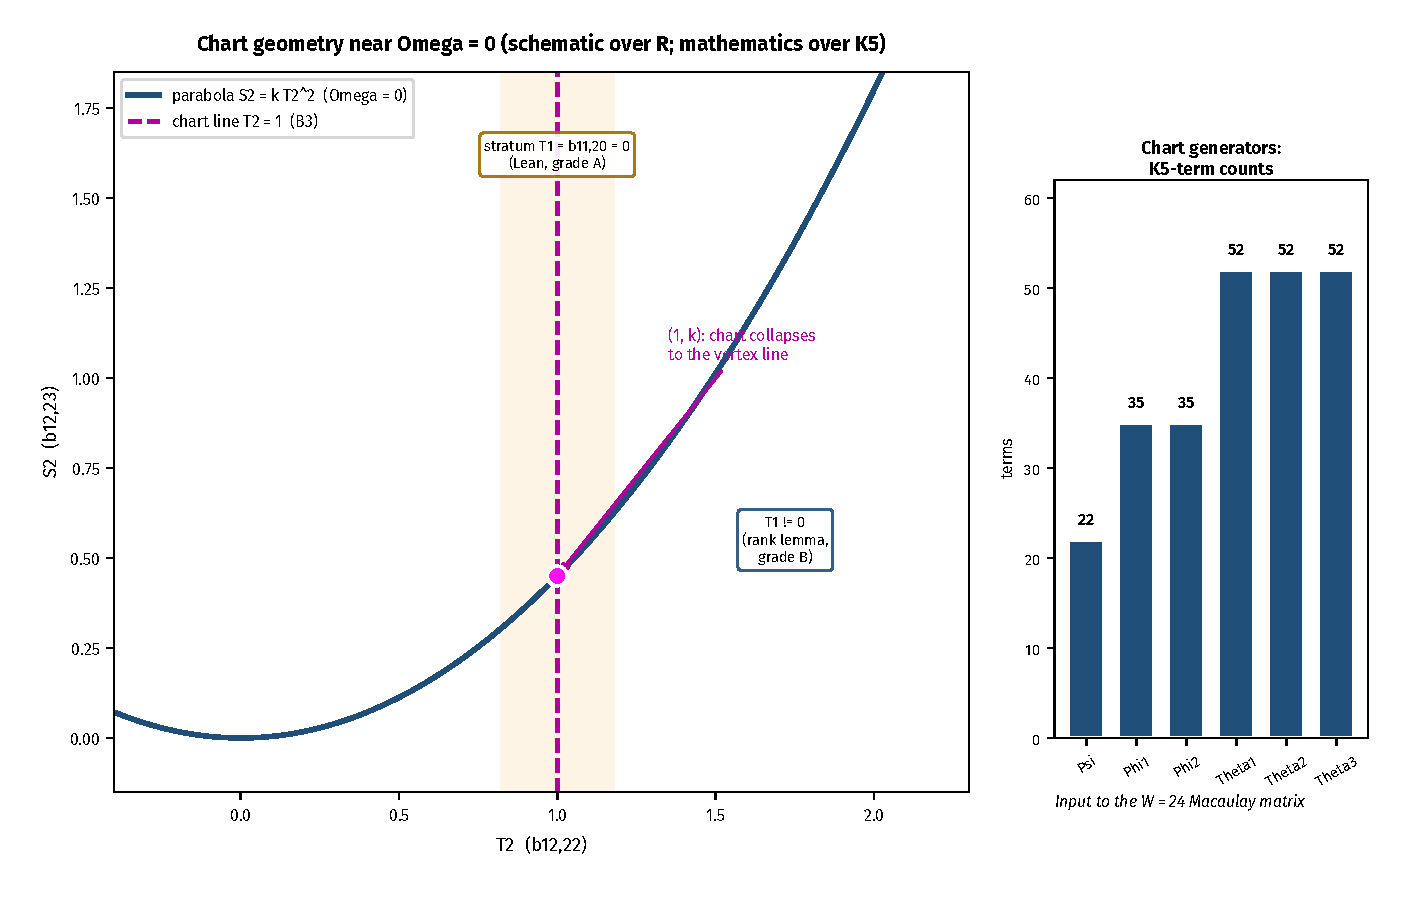
\includegraphics[width=0.95\textwidth]{figures_c/fig3_omega.pdf}
\caption{The chart near $\Omega=0$. Main panel: the $(T_2,S_2)$-plane, drawn schematically over $\mathbb{R}$ (the mathematics is over $K_5$), with the parabola $S_2=\kappa T_2^2$ of~\eqref{bc:eq:omegafactor}, the chart line $T_2=1$ of Step~B3, and their intersection $(1,\kappa)$. The stratum $T_1=b_{11,20}=0$ is indicated as a transverse slice; it is eliminated in Lean (\S\ref{bc:sec:t1zero}), and the stratum $T_1\neq0$ is eliminated by the rank lemma (grade~B) and by the Lean certificate (grade~A). Inset: the numbers of $K_5$-terms of the six chart generators ($22,35,35,52,52,52$), which are the input to the Macaulay matrix of \S\ref{bc:sec:wholechart}. Drawn by \texttt{figures/fig3\_\allowbreak{}omega.\allowbreak{}py}.}
\label{bc:fig:omega}
\end{figure}

\section{\texorpdfstring{The stratum $b_{11,20}=0$}{The stratum b11,20=0}}\label{bc:sec:t1zero}

\emph{Step B7} (Lean kernel). On the stratum $T_1=b_{11,20}=0$ the twelve conditions have no common zero, and there is an explicit proof of this small enough for the kernel. A \emph{certificate} of emptiness is a list of polynomial multipliers $c_n$ with $\sum_nc_nF_n$ equal to a nonzero constant, where the $F_n$ are the conditions together with $T_1$, $T_2-1$ and $R(w)$. Such an identity forbids a common zero, since at a common zero the left side vanishes and the right side does not. On this stratum a certificate of degree~$2$ exists, with $75$ terms over $K_5$ and coefficients of at most $9{,}681$ digits (\filename{chart\_certificates/step1/certB\_lowerc.json}). It was produced by \filename{certB\_lowerc.py}, which chooses pivots from a reduced row-echelon form modulo a prime and then solves exactly with FLINT, and it was rechecked by \filename{check\_certB\_lowerc.py}, which expands it with \texttt{fmpq\_\allowbreak{}mpoly}, treating $w$ as a variable and reducing modulo $R$ at the end. The directory \filename{Jacobian/BranchC/T1Zero}, generated by \filename{gen\_t1zero\_lean.py}, checks the whole chain in the kernel, in the steps of Table~\ref{bc:tab:t1zero}.

\begin{table}[htbp]
\centering
\footnotesize
\begin{tabular}{>{\raggedright\arraybackslash}p{0.13\textwidth}>{\raggedright\arraybackslash}p{0.62\textwidth}l}
\toprule
Step & Identity (between integer polynomials, kernel-checked) & Build time \\
\midrule
\texttt{s\_\allowbreak{}sq} & $D_OD_{o_1}D_k^2\,\Omega\equiv D_ON_{o_1}X^2\bmod(T_2-1,R)$, where $X=D_kS_2-N_\kappa(w)$ and $D_k=851565312$ & $1.5$~s \\
\texttt{s\_\allowbreak{}X2} & Bezout identity $a\cdot e_{\mathrm{sq}}+b\cdot D_OX^2R=c\cdot D_OX^2$ with $c$ of $151$ digits; hence $X=0$ & --- \\
\texttt{s\_\allowbreak{}f\_\allowbreak{}n} (six) & $D_k^d\cdot ck_n=D_k^dT_1A_1+D_k^d(T_2-1)A_2+XA_3+f_n+RA_4$ & $2.4$--$5.7$~s \\
\texttt{s\_\allowbreak{}p\_\allowbreak{}n} (six) & $p_n=\nu_nf_n-q_nR$ ($250$--$375$ terms, about $5{,}440$ digits) & $17$--$28$~s \\
\texttt{s\_\allowbreak{}final} & $\sum_np_n=DD$, an exact integer of $5387$ digits & $55.6$~s \\
\bottomrule
\end{tabular}
\caption{The kernel-checked chain for the stratum $b_{11,20}=0$ (files \texttt{Sq.\allowbreak{}lean}, \texttt{F\_\allowbreak{}*.\allowbreak{}lean}, \texttt{P\_\allowbreak{}*.\allowbreak{}lean} and \texttt{Final.\allowbreak{}lean} in \texttt{Jacobian/BranchC/T1Zero}).}
\label{bc:tab:t1zero}
\end{table}

In words: the first two steps use $\Omega=0$ and $T_2=1$ to obtain $X=0$, that is $S_2=\kappa$. The steps \texttt{s\_\allowbreak{}f\_\allowbreak{}n} rewrite each of the six conditions $\Psi,\Phi_1,\Phi_2,\Theta_1,\Theta_2,\Theta_3$, modulo $T_1$, $T_2-1$, $X$ and $R$, as a polynomial $f_n$ in the remaining variables. The steps \texttt{s\_\allowbreak{}p\_\allowbreak{}n} multiply by the certificate coefficients and reduce modulo $R$, and \texttt{s\_\allowbreak{}final} shows that the products add up to the integer $DD$. The theorem \texttt{chartEmpty\_\allowbreak{}t1\_\allowbreak{}zero} (\filename{Jacobian/BranchC/T1Zero/Main.lean}) chains these steps. At a common zero all the left sides vanish, so $DD=0$ in $L$, which contradicts characteristic~$0$; the module builds in $26$~s under \texttt{lake}. The hypotheses of \texttt{chartEmpty\_\allowbreak{}t1\_\allowbreak{}zero} are exactly the \texttt{cond\_\allowbreak{}*} of \filename{CondsC.lean}, which are by definition the conditions that \filename{Descent2R} derives. Five perturbed copies of the chain serve as negative controls: Bezout constant plus one, one equation dropped, one cofactor coefficient changed, $DD+1$ in place of $DD$, and the equation $T_2=1$ dropped. The kernel rejects all five (\filename{logs/t1z\_controls.log}: five of five fail, as required).

\emph{Step B6} (Lean). The theorem \texttt{chartEmptyC\_\allowbreak{}of\_\allowbreak{}\allowbreak T1ne0} (\filename{Jacobian/BranchC/T1Zero/Combine.lean}, line~41) splits the chart according to whether $b_{11,20}=0$. On that stratum it applies \texttt{chartEmpty\_\allowbreak{}t1\_\allowbreak{}zero}; on its complement it applies the hypothesis \texttt{ChartEmptyC\_\allowbreak{}T1ne0}. So \texttt{ChartEmptyC\_\allowbreak{}T1ne0} implies \texttt{ChartEmptyC}, and the part of the chart statement that this split leaves open is the proposition of Listing~\ref{bc:lst:chartempty}.

\begin{leanlisting}{\texttt{ChartEmptyC\_T1ne0}: the stratum $b_{11,20}\neq0$, proved in Lean by \texttt{challenge\_target} (Theorem~\ref{bc:thm:unconditional})}{bc:lst:chartempty}
-- Jacobian/BranchC/T1Zero/Combine.lean (statement with ten of the twelve condition hypotheses elided)
def ChartEmptyC_T1ne0 (L : Type*) [Field L] : Prop :=
  ∀ (w : L), w ^ 5 - w ^ 4 + 3 * w ^ 3 + 3 * w ^ 2 + 26 = 0 →
  ∀ (b_11_20 b_12_22 b_11_21 b_12_23 a_6_13 a_7_15 b_10_21 : L), b_12_22 = 1 → b_11_20 ≠ 0 →
    cond_Omega w b_11_20 b_12_22 b_11_21 b_12_23 a_6_13 a_7_15 b_10_21 = 0 →
    ...
    cond_Em2pure_17_37 w b_11_20 b_12_22 b_11_21 b_12_23 a_6_13 a_7_15 b_10_21 = 0 → False
\end{leanlisting}

\section{The whole chart}\label{bc:sec:wholechart}

On the whole chart we no longer use $T_1=0$, and a certificate of the kind used in \S\ref{bc:sec:t1zero} becomes too large to compute on the machine available. We call the identity $1=\sum_nc_nF_n$ for the whole chart the \emph{canonical certificate}. Its size can be estimated. At weight $W=24$ (defined below) Hadamard's inequality bounds the coefficient heights of its solution by $4{,}392{,}160$ digits. On the slices with $t_1=0$ at $W=2,3,4$ the actual heights are $0.061$, $0.061$ and $0.046$ times the bound, and calibrating with these ratios predicts heights of $2.0$--$2.7\times10^5$ digits per coefficient, about $2\times10^9$ digits in all. The Hadamard bound is rigorous; the calibrated prediction is a grade-C estimate. An exact solution ran out of memory at $7$~GB, and multimodular reconstruction would need about $3\times10^4$ primes at $15$--$20$~s each, about six days of computation. Instead of exhibiting the canonical certificate we prove that it exists. The determinant of the square submatrix $M_S$ that carries the argument is a different object, and it has been computed exactly (\S\ref{bc:sec:detvalue}); the canonical certificate itself has not been exhibited.

\subsection{Macaulay matrices and the rank lemma}

We first eliminate two variables. By~\eqref{bc:eq:omegafactor}, on the chart $T_2=1$ and $S_2=\kappa$. Substituting these values into $\Psi,\Phi_1,\Phi_2,\Theta_1,\Theta_2,\Theta_3$ gives six polynomials $F_1,\dots,F_6\in K_5[T_1,S_1,R_1,R_2,Q]$, the \emph{chart generators}, with $22,35,35,52,52,52$ terms over $K_5$. Give $T_1,S_1,R_1,R_2,Q$ the weights $1,2,3,3,4$ of the table above, write $\operatorname{wdeg}$ for the weighted degree of a monomial, and let $\operatorname{wt}F_n$ be the weight of the condition from which $F_n$ comes ($5$ for $\Psi$, $6$ for $\Phi_1,\Phi_2$, $7$ for $\Theta_1,\Theta_2,\Theta_3$). The five pure rows are not used.

The \emph{Macaulay matrix} of weight $W$ records the linear algebra of the equation $1=\sum_nc_nF_n$ with $\operatorname{wdeg}c_n\le W-\operatorname{wt}F_n$. Its columns are indexed by the pairs $(n,m)$ with $m$ a monomial in $T_1,S_1,R_1,R_2,Q$ and $\operatorname{wdeg}m\le W-\operatorname{wt}F_n$; its rows are indexed by the monomials that occur in the products $m\cdot F_n$, together with the monomial $1$; and the entry in row $\mu$ and column $(n,m)$ is the coefficient of $\mu$ in $m\cdot F_n$. A vector $x$ with $Mx=e_1$, where $e_1$ is the unit vector of the row of the monomial $1$, is exactly a list of multipliers with $\sum_nc_nF_n=1$. If $M$ has full row rank, that is, rank equal to its number $N$ of rows, its columns span the whole space of row vectors, so such an $x$ exists. We reproduced the sizes of these matrices from \filename{conds\_c.json} and $\kappa$: at $W=22$ there are $2281$ rows and $3934$ columns, at $W=23$ there are $2708$ rows and $4904$ columns, and at $W=24$ there are $3199$ rows and $6054$ columns (\filename{c2\_k5\_chart\_macaulay.py}, exit code~$0$).

\begin{lemma}[Fixed-degree Macaulay rank lifts]\label{bc:lem:rank}
Let $p$ be a prime, $\mathbb{Z}_{(p)}$ the ring of rational numbers with denominator prime to $p$, and $A=\mathbb{Z}_{(p)}[w]/(R)$. Then $A$ is free of rank~$5$ over $\mathbb{Z}_{(p)}$ and embeds in $K_5$. Let $w_0\in\mathbb{Z}$ satisfy $R(w_0)\equiv0\pmod p$, and let $\varphi_p:A\to\mathbb{F}_p$ be the ring homomorphism with $w\mapsto w_0$. Let $M$ be the Macaulay matrix of the chart generators at a fixed weight $W$, and assume that its entries lie in $A$. If $\varphi_p(M)$ has full row rank $N$ over $\mathbb{F}_p$, then $M$ has full row rank $N$ over $K_5$.
\end{lemma}

\begin{proof}
Since $R$ is monic of degree $5$, the classes of $1,w,\dots,w^4$ form a basis of $A$ over $\mathbb{Z}_{(p)}$, and $A\to A\otimes_{\mathbb{Z}_{(p)}}\mathbb{Q}=K_5$ is injective because $A$ is torsion-free. The map $\varphi_p$ is well defined because $R(w_0)\equiv0\pmod p$. As $\varphi_p(M)$ has rank $N$, some set $S$ of $N$ columns gives an $N\times N$ submatrix with $\det\varphi_p(M_S)\neq0$. The determinant is a polynomial with integer coefficients in the entries and $\varphi_p$ is a ring homomorphism, so $\varphi_p(\det M_S)=\det\varphi_p(M_S)\neq0$. Hence $\det M_S\neq0$ in $A$, and so in the field $K_5$, where $M_S$ is therefore invertible. Its $N$ columns are linearly independent, and $M$ has rank $N$ over $K_5$.
\end{proof}

If the hypothesis holds at $W=24$, the equation $Mx=e_1$ is solvable over $K_5$, so $1=\sum_nc_nF_n$ in $K_5[T_1,S_1,R_1,R_2,Q]$ with $\operatorname{wdeg}c_n\le24-\operatorname{wt}F_n$. Now let $L$ be any field of characteristic~$0$ and $w\in L$ a root of $R$. Sending the class of $w$ to this root embeds $K_5$ in $L$, and the identity maps to an identity in $L[T_1,S_1,R_1,R_2,Q]$, so $F_1,\dots,F_6$ have no common zero over $L$. Together with $S_2=\kappa$, which follows from $\Omega=0$ and $o_1\neq0$ by~\eqref{bc:eq:omegafactor}, no point of the chart satisfies $\Omega=\Psi=\Phi_1=\Phi_2=\Theta_1=\Theta_2=\Theta_3=0$. This is \texttt{ChartEmptyC}, and a fortiori \texttt{ChartEmptyC\_\allowbreak{}T1ne0}; it holds without the five pure rows and without the restriction $b_{11,20}\neq0$.

\begin{remark}[Why this lemma succeeds where the retracted one failed]
That the Macaulay system has a solution modulo~$p$ says only that it is consistent modulo~$p$, and consistency does not lift: $1+109X$ over $\mathbb{Z}_{(109)}$ is the example of Remark~\ref{bc:rem:retraction}. Full row rank at a fixed degree is the nonvanishing of a minor, and that does lift, by the proof above. The planted-zero control below shows how sensitive the test is: a single common zero lowers the rank by exactly one.
\end{remark}

\subsection{The instance}

The script \filename{step3b\_rank\_lift.py} ran in $6.4$~minutes using $0.5$~GB of memory (log \filename{step3b\_rank\_lift.log}; the log records a runtime of $384.3$~s). Table~\ref{bc:tab:ranks} gives its results at the two primes of~\eqref{bc:eq:primes} with large $p$. In each row ``rank'' is the rank of $\varphi_p(M)$, and ``augmented'' is the rank after the column $e_1$ is adjoined; when the augmented rank exceeds the rank, $e_1$ is not in the column space and the weight-$W$ equation $1=\sum c_nF_n$ has no solution modulo~$p$.

\begin{table}[htbp]
\centering
\small
\begin{tabular}{>{\raggedright\arraybackslash}p{0.36\textwidth}>{\raggedright\arraybackslash}p{0.3\textwidth}l}
\toprule
 & $p=1000003$, $w_0=806739$ & $p=32003$, $w_0=11147$ \\
\midrule
all coefficients $p$-integral, $R(w_0)\equiv0$ & checked & checked \\
$W=22$: rank / augmented / rows & $2277/2278/2281$: no solution & same \\
$W=23$: rank / augmented / rows & $2707/2708/2708$: no solution & same \\
$W=24$: $3199\times6054$ & $3199/3199/3199$: full row rank & same \\
independent NumPy pivot-block elimination & $\det\neq0$ & $\det\neq0$ \\
planted common zero at $W=24$ (control) & rank $3198$, no solution & same \\
\bottomrule
\end{tabular}
\caption{Ranks of the reduced Macaulay matrices. Data: \texttt{step3b\_\allowbreak{}rank\_\allowbreak{}lift.\allowbreak{}log}.}
\label{bc:tab:ranks}
\end{table}

The protocol was fixed before the run: the lemma, the second prime, the independent NumPy elimination and the controls were all written into \filename{step3b\_rank\_lift.py} before it was executed. The threshold $W=24$ is sharp, since at $W=22$ and $W=23$ the equation has no solution (Figure~\ref{bc:fig:ranks}). The chart generators were checked separately to be the right polynomials by \filename{step3c\_chart\_identity.py}: by exact evaluation at $12$ random points, by an independent computation of $\kappa$, by the exact square~\eqref{bc:eq:omegafactor}, and by controls, among them the substitution of $\kappa+1$ for $\kappa$, which is detected. We call this argument, carried out outside Lean, \emph{Step B8}; its grade is~B.

\begin{figure}[htbp]
\centering
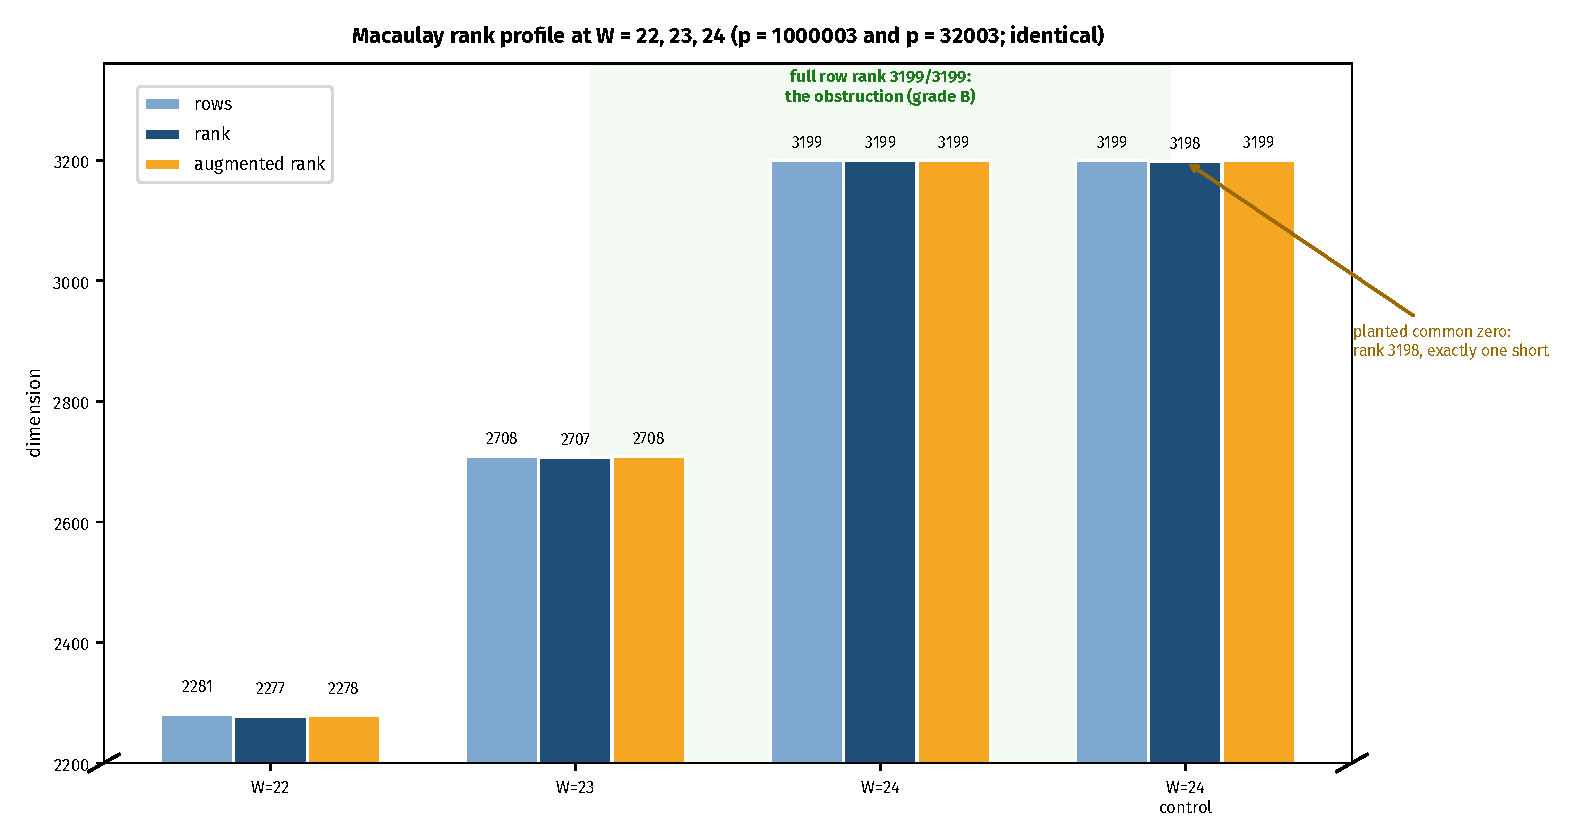
\includegraphics[width=0.95\textwidth]{figures_c/fig4_ranks.pdf}
\caption{Rank profile of the Macaulay matrices at weights $W=22,23,24$, identical at $p=1000003$ and $p=32003$. For each weight the bars give the number of rows ($2281$, $2708$, $3199$), the rank ($2277$, $2707$, $3199$) and the augmented rank; the group $W=24$, where the rank is full ($3199/3199$), is highlighted. The fourth group is the planted-common-zero control at $W=24$ (rank $3198$, one short of full). Data: \texttt{step3b\_\allowbreak{}rank\_\allowbreak{}lift.\allowbreak{}log}. Drawn by \texttt{figures/fig4\_\allowbreak{}ranks.\allowbreak{}py}; the vertical axis is truncated, with a break mark, to make the deficit of one visible.}
\label{bc:fig:ranks}
\end{figure}

\subsection{The rank argument inside Lean}\label{bc:sec:leanrank}

The theorem \texttt{challenge\_\allowbreak{}target} of Theorem~\ref{bc:thm:unconditional} is the argument of the rank lemma at the prime $p=32003$, written so that every step is checked by the kernel. Its core is \texttt{chartEmptyC\_\allowbreak{}T1ne0\_\allowbreak{}of\_\allowbreak{}\allowbreak certificate} (\filename{branch\_c/grade\_a/lean/GradeA/Chart/Assembly.lean}, line~73), and its structure is as follows.

The entries of the Macaulay matrix are taken in $\mathbb{Z}[X]$, with $X$ standing for $w$; the generators are scaled by integers so that their coefficients are integer polynomials in $w$. Let $\rho$ be an index set with $3199$ elements (\texttt{Fin 3199}), and let a square submatrix $M_S$ be specified by an injective list of $3199$ row monomials, one of which is the monomial $1$ (hypotheses \texttt{hmon} and \texttt{hr\_\allowbreak{}1}), and by $3199$ columns $(n,m)$ (the maps \texttt{gen} and \texttt{mult}). The hypothesis \texttt{hsupp2} states that every monomial of every product $m\cdot F_n$ in a chosen column is one of the listed row monomials. Suppose that $L$ has characteristic~$0$ and that $w\in L$ and a chart point are a common zero. Then the row vector $v$ of the values of the row monomials at that point has entry $1$ at the monomial $1$, so it is nonzero, and $v\,M_S(w)=0$ because each column of $M_S(w)$ lists the coefficients of a polynomial $m\cdot F_n$ that vanishes at the point (\texttt{macaulay\_\allowbreak{}vecMul\_\allowbreak{}eq\_\allowbreak{}zero}, \filename{Macaulay.lean}, line~66). So $\det M_S$, an element of $\mathbb{Z}[X]$, vanishes at $w$. Since $R$ is irreducible over $\mathbb{Q}$ (proved in Lean through its reduction modulo $67$, \filename{IrreducibleR.lean}), it is the minimal polynomial of $w$, so $R$ divides $\det M_S$ in $\mathbb{Q}[X]$, and since $R$ is monic it divides it in $\mathbb{Z}[X]$. Reducing modulo $p$ and evaluating at $w_0=11147$, where $R(w_0)\equiv0\pmod{32003}$, we get $\det M_S(w_0)\equiv0\pmod p$ (\filename{Transfer.lean}, \texttt{eval\_\allowbreak{}eq\_\allowbreak{}zero\_\allowbreak{}of\_\allowbreak{}eval\_\allowbreak{}root} and \texttt{no\_\allowbreak{}left\_\allowbreak{}kernel}). On the other hand two hypotheses checked by the kernel on explicit data assert that the reduction of $M_S$ is invertible. The first, A2, states that the reduced block equals a $3199\times3199$ matrix \texttt{MS} over $\mathbb{F}_{32003}$ times a diagonal matrix of nonzero column scalings (\filename{A2Assembly.lean}, line~169). The second, A1, states $\texttt{Cinv}\cdot\texttt{MS}=1$ for an explicit matrix \texttt{Cinv} (\filename{A1Instantiation.lean}, line~328). Together they contradict $\det M_S(w_0)\equiv0$. The chart generators used in this argument (\texttt{Fpoly}) are identified with the generators of the descent by \texttt{bridge\_\allowbreak{}Fpoly}: both are the same six \texttt{polyOfTerms} expressions, in the same order, built from the single definitions \texttt{tl\_\allowbreak{}*} of \filename{Chart/Gens.lean}.

The Lean proof differs from the argument of Lemma~\ref{bc:lem:rank} in two respects. It never uses $b_{11,20}\neq0$ or the five pure rows, so it proves more than \texttt{ChartEmptyC\_\allowbreak{}T1ne0}. And it replaces the passage through $A=\mathbb{Z}_{(p)}[w]/(R)$ in Lemma~\ref{bc:lem:rank} by the divisibility of an integer polynomial by $R$, which uses the irreducibility of $R$ and avoids localization. Of the data hypotheses, only A1, A2 and \texttt{hsupp2} at the concrete data $p=32003$, $w_0=11147$, $\rho=\mathtt{Fin}\ 3199$ are proved by kernel computation on large explicit matrices; they are the kernel-verified part of the certificate. The rank computation at $p=1000003$ and the NumPy elimination of Table~\ref{bc:tab:ranks} remain an independent check at grade~B.

\subsection{The value of the determinant}\label{bc:sec:detvalue}

The determinant $\det M_S\in K_5$ has since been computed exactly. A multimodular reconstruction, run on November~10 and~11, 2026, recovered it as five rational coefficients with respect to the basis $1,w,\dots,w^4$, with numerators of $1{,}124{,}076$ to $1{,}124{,}083$ bits and denominators of $1{,}089{,}696$ to $1{,}089{,}704$ bits. The method computes $\det M_S$ modulo many $61$-bit primes, combines the residues by the Chinese remainder theorem and recovers the rational coefficients by lattice reduction (Kannan's embedding with LLL). The same value was obtained in two verification attempts, one with $244{,}000$ equations and a modulus $M$ of $14{,}884{,}000$ bits, the other with $250{,}000$ equations and $M$ of $15{,}250{,}000$ bits. The common denominator has $2{,}800{,}648$ bits. The value is filed as \filename{gghv-dependency-closure/leg9/result.json} (sha256 \filename{e7813e7896fff29466461446ded89499e4dd17f8d7d2ccc9a071e8903e96795c}) and deposited under DOI 10.5281/zenodo.24157382. It reproduces the determinant values at six primes known beforehand, namely $32003$, $1000003$, $100003$, $500009$, $999983$ and $2^{61}-1$, none of which was used in the reconstruction, and at ten further primes chosen after the reconstruction. At three further small primes the value was checked independently in Singular, with Singular and FLINT agreeing (November~11, 2026). In particular $\det M_S\neq0$ in $K_5$, as Lemma~\ref{bc:lem:rank} already implies; the computation adds the exact value to the nonvanishing. The square submatrix is named by its row and column indices, its determinant is nonzero and its value is exhibited, which is what an explicit-minor certificate requires. The canonical certificate $1=\sum_nc_nF_n$ is still not exhibited. The value is a computational identification and is recorded as such (Table~\ref{bc:tab:grades}, C11); it changes no grade and no theorem.

\section{Proof of the main theorem}\label{bc:sec:proof}

\begin{leanlisting}{\texttt{main\_theorem\_c\_of\_\allowbreak chartEmpty\_T1ne0}}{bc:lst:main}
-- Jacobian/BranchC/T1Zero/Combine.lean, line 53 (statement verbatim)
theorem main_theorem_c_of_chartEmpty_T1ne0 {L : Type*} [Field L] [CharZero L]
    (h : ChartEmptyC_T1ne0 L) :
    ¬ ∃ (P Q : MvPolynomial (Fin 2) L) (lam : L), lam ≠ 0 ∧ NewtonNFc P Q ∧
      jac P Q = C lam * X 0 ^ 2 :=
  main_theorem_c_of_claim (descentClaimC_of_chartEmpty_T1ne0 L h)
\end{leanlisting}

\begin{proof}[Proof of Theorem~\ref{bc:thm:main}]
Let $P,Q\in L[x,y]$ and $\lambda\neq0$ satisfy \texttt{NewtonNFc}$(P,Q)$ and $[P,Q]=\lambda x^2$. Step~B0 gives the layer identities $E_n$. Step~B1 identifies the top layer with the $K_5$ solution, Step~B2 gives $t_2\neq0$, and Step~B3 transports the data to the chart $b_{12,22}=1$. The result satisfies the hypotheses of \texttt{DescentClaimC}: $19$ top-layer values, $123$ unknowns and the layer identities. Step~B4 extracts the $132$ scalar equations, and Step~B5 (\texttt{chart\_\allowbreak{}descent\_\allowbreak{}refl}) derives from them the vanishing of the twelve conditions, so the data give a point of the chart, which \texttt{ChartEmptyC} forbids. Step~B6 splits on $b_{11,20}$. If $b_{11,20}=0$, Step~B7 (\texttt{chartEmpty\_\allowbreak{}t1\_\allowbreak{}zero}) gives \texttt{False} in the kernel. If $b_{11,20}\neq0$, the hypothesis \texttt{ChartEmptyC\_\allowbreak{}T1ne0} gives \texttt{False}. Hence no such $P,Q,\lambda$ exist.
\end{proof}

Theorem~\ref{bc:thm:unconditional} and Corollary~\ref{bc:cor:unconditional} follow by supplying \texttt{ChartEmptyC\_\allowbreak{}T1ne0} from \texttt{challenge\_\allowbreak{}target} (\S\ref{bc:sec:leanrank}); the rank route of \S\ref{bc:sec:wholechart} supplies it independently at grade~B. Corollary~\ref{bc:cor:gghv} follows by applying \cite[Prop.~4.3]{GGHV}. Table~\ref{bc:tab:bridges} summarizes the composition.

\begin{table}[htbp]
\centering
\small
\begin{tabular}{l>{\raggedright\arraybackslash}p{0.22\textwidth}>{\raggedright\arraybackslash}p{0.18\textwidth}>{\raggedright\arraybackslash}p{0.31\textwidth}c}
\toprule
Step & From & To & Lean name & Grade \\
\midrule
B0 & $[P,Q]=\lambda x^2$, \texttt{NewtonNFc} & layer identities $E_n$ & \texttt{layers\_\allowbreak{}of\_\allowbreak{}jac\_\allowbreak{}c} & A \\
B1 & $E_5$, vertices & $K_5$ top layer & \texttt{eIdent\_\allowbreak{}five}, \texttt{chartClassification\_\allowbreak{}holds} & A \\
B2 & B0, B1 & $t_2=b_{12,22}\neq0$ & \texttt{vertex\_\allowbreak{}12\_\allowbreak{}24\_\allowbreak{}forces\_\allowbreak{}t2}, \texttt{degree19\_\allowbreak{}rigidity} & A \\
B3 & B0--B2 & chart $b_{12,22}=1$ & \texttt{eIdent\_\allowbreak{}transport}, \texttt{main\_\allowbreak{}theorem\_\allowbreak{}c\_\allowbreak{}of\_\allowbreak{}claim} & A \\
B4 & $E_n$, $n=4,\dots,-2$ & $132$ scalar equations & \texttt{eIdent\_\allowbreak{}c4}, \dots, \texttt{eIdent\_\allowbreak{}cm2} & A \\
B5 & $132$ equations & twelve conditions & \texttt{chart\_\allowbreak{}descent\_\allowbreak{}refl} & A \\
B6 & \texttt{ChartEmptyC\_\allowbreak{}T1ne0} & \texttt{ChartEmptyC} & \texttt{chartEmptyC\_\allowbreak{}of\_\allowbreak{}\allowbreak T1ne0} & A \\
B7 & conditions, $b_{11,20}=0$ & \texttt{False} & \texttt{chartEmpty\_\allowbreak{}t1\_\allowbreak{}zero} & A \\
B8 & chart generators & \texttt{False} & rank lemma and \filename{step3b\_rank\_lift.py} (outside Lean) & B \\
\bottomrule
\end{tabular}
\caption{The steps of the proof and their grades.}
\label{bc:tab:bridges}
\end{table}

Step~B8 corroborates and is no longer needed for the proof: \texttt{challenge\_\allowbreak{}target} discharges \texttt{ChartEmptyC\_\allowbreak{}T1ne0} at grade~A. The grades of B0--B7, and of B8 as it was proved, are unchanged.

\section{Epistemic status and what is not claimed}\label{bc:sec:epistemic}

Every claim of this Part carries a grade, in the scheme described in Appendix~\ref{app:methods}. In brief, grade~A means a proof checked by the Lean kernel or an exact deduction from stated axioms, grade~B a derivation under explicitly stated premises, which here are computations carried out outside the kernel, grade~C a heuristic or fitted estimate, and grade~D a statement that is tautological or refuted. The label F1 marks a computational identification recorded as a step, and the independence label I1 means the identification has not been reproduced by an independent party. Table~\ref{bc:tab:grades} lists the claims.

\begin{table}[htbp]
\centering
\small
\begin{tabular}{@{}l>{\raggedright\arraybackslash}p{0.38\textwidth}>{\raggedright\arraybackslash}p{0.42\textwidth}c@{}}
\toprule
ID & Claim & Evidence & Grade \\
\midrule
C1 & \texttt{main\_\allowbreak{}theorem\_\allowbreak{}c\_\allowbreak{}of\_\allowbreak{}claim} & Lean kernel & A \\
C2 & \texttt{descentClaimC\_\allowbreak{}of\_\allowbreak{}\allowbreak chartEmpty} & Lean kernel, by reflection; the $600$ identities also checked in Python & A \\
C3 & \texttt{chartEmpty\_\allowbreak{}t1\_\allowbreak{}zero} & Lean kernel; FLINT certificate rechecked in Python; five negative controls & A \\
C4 & \texttt{chartEmptyC\_\allowbreak{}of\_\allowbreak{}\allowbreak T1ne0} & Lean kernel & A \\
C5 & \texttt{ChartEmptyC} holds for every field of characteristic~$0$ & Lean: \texttt{challenge\_\allowbreak{}target} with \texttt{chartEmptyC\_\allowbreak{}of\_\allowbreak{}\allowbreak T1ne0} (November~4, 2026); independently, the rank lemma with ranks at two primes by two implementations and checks of the inputs (grade~B) & A \\
C6 & the canonical certificate needs about $2\times10^9$ digits & Hadamard bound (rigorous) times a calibrated ratio (fitted) & C \\
C7 & the reduction lemma as stated is inconsistent & Lean derivation of \texttt{False} from it, via $1+109X$ & A \\
C8 & the ideal of \filename{lower\_c.py} differs from that of the earlier pipeline & exact comparison & A \\
C9 & \texttt{ChartEmptyC\_\allowbreak{}T1ne0} holds for every field of characteristic~$0$, with no hypotheses & Lean: \texttt{challenge\_\allowbreak{}target} (identification of generators with A1, A2, \texttt{hsupp2}) & A \\
C10 & branch~(c) is eliminated: no \texttt{NewtonNFc} pair with $[P,Q]=\lambda x^2$, $\lambda\neq0$ & Lean: \texttt{branch\_\allowbreak{}c\_\allowbreak{}eliminated}, from C9 and \texttt{main\_\allowbreak{}theorem\_\allowbreak{}c\_\allowbreak{}of\_\allowbreak{}\allowbreak chartEmpty\_\allowbreak{}T1ne0} & A \\
C11 & $\det M_S$ exhibited as an explicit element of $K_5$ & multimodular reconstruction, filed as \filename{gghv-dependency-closure/leg9/result.json} (DOI 10.5281/zenodo.24157382); six known values and ten fresh primes; three fresh small primes checked in Singular; step record, I1 & F1 \\
\bottomrule
\end{tabular}
\caption{Claims of Part~II and their grades.}
\label{bc:tab:grades}
\end{table}

The verbs of the text follow the grades. We say ``proves'' only for kernel-checked or exact deductions, ``proves under stated computational premises'' for the rank route B8, and ``estimates'' for C6.

Several things are not claimed. We do not claim the planar Jacobian conjecture. We do not claim any other case of \cite[Prop.~4.3]{GGHV}, nor the reduction from the conjecture to that proposition. We do not claim that $(72,108)$ is excluded unconditionally; that needs the correctness and exhaustiveness of \cite[Prop.~4.3]{GGHV}, which we record as premises and do not re-derive. We do not claim an explicit certificate over $K_5$ for the whole chart: such a certificate exists by the rank lemma, and the load-bearing whole-chart step is the Lean certificate C9, not an exhibited certificate over $K_5$. The determinant of C11 is a different object from that whole-chart certificate; the former is exhibited and the latter is not. We have not reviewed the deferred single-prime $p$-adic argument or the retracted \texttt{char0\_\allowbreak{}cert} bundle. The Gr\"obner and lifting certificates over $\mathbb{F}_{101}$, $\mathbb{F}_{1000003}$ and $\mathbb{F}_{109^5}$ are certificates and not proofs: each excludes only those solutions that are integral at its prime. What lifts to characteristic~$0$ is the rank argument.

The open items are these. (1)~An independent replication of the rank computation of Step~B8: a rank computation of the $W=24$ Macaulay matrix in Magma, Sage or Singular, starting from \filename{conds\_c.json} and $\kappa$. (2)~A Lean formalization of the rank argument has been carried out at $p=32003$ (\S\ref{bc:sec:leanrank}); a formalization at the second prime $1000003$ has not. (3)~The deferred reviews named above. (4)~A corrected commit of the directory \filename{branch\_c/}, to be made only on the author's explicit decision. (5)~Further independent checks of the value of $\det M_S$ against \filename{gghv-dependency-closure/leg9/result.json}: the check at three fresh small primes in Singular is done, while checks at more primes, in Magma or Sage, or at fresh $61$-bit primes by an independent implementation remain open. A Lean formalization of the value itself is a separate task and is not scheduled. The tracking of \texttt{challenge\_\allowbreak{}target} and \texttt{branch\_\allowbreak{}c\_\allowbreak{}eliminated} as repository modules, listed as open in an earlier version, was done on November~6, 2026 (\S\ref{bc:sec:modules}).

\section{The Lean modules}\label{bc:sec:modules}

The branch-(c) development lives in the directory \filename{Jacobian/BranchC/} of the Lean project \filename{branch\_c/bundle\_v3\_1/jacobian\_lean}, which contains $686$ files. They fall into the groups of Table~\ref{bc:tab:modules}. The full build of the project, which also contains the branch-(a,b) modules it imports, comprises $790$ modules, all up to date in the final verification log (\filename{bundle\_v3\_1/logs/verify\_v3.log}). The directory \filename{Descent2R} contains $506$ files: the bridge \filename{Bridge.lean}, the main file \filename{Main.lean}, and $504$ generated reflection modules, namely \filename{Facts.lean}, six files \filename{Vals\_*.lean} and the $497$ layer modules of Table~\ref{bc:tab:descent} ($54+57+57+60+60+99+110=497$). The two tracked modules \texttt{GradeA.\allowbreak{}Bridge} and \texttt{GradeA.\allowbreak{}Composition}, which contain \texttt{challenge\_\allowbreak{}target} and \texttt{branch\_\allowbreak{}c\_\allowbreak{}eliminated}, live in the separate project \filename{branch\_c/grade\_a/lean} together with the data files for A1, A2 and \texttt{hsupp2}.

\begin{table}[htbp]
\centering
\small
\begin{tabular}{>{\raggedright\arraybackslash}p{0.3\textwidth}>{\raggedright\arraybackslash}p{0.5\textwidth}r}
\toprule
Group & Contents & Files \\
\midrule
top level (first and second versions) & \filename{Degree19}, \filename{DescentClaim}, \filename{Edge19}, \filename{LayerE2}, \filename{LayersGen}, \filename{OmegaEdge}, \filename{OmegaSquare} & $7$ \\
\filename{Descent/} & first descent formalization & $59$ \\
\filename{Rank/} & operator-rank theorems & $96$ \\
\filename{CondsC.lean}, \filename{Descent2R/Bridge.lean} & the twelve conditions; B4 and \texttt{ChartEmptyC} & $2$ \\
\filename{Descent2R/} other than \filename{Bridge.lean} & $504$ generated reflection modules and \filename{Main.lean} & $505$ \\
\filename{T1Zero/} & $15$ certificate modules and \filename{Main.lean}, then \filename{Combine.lean} & $17$ \\
\midrule
total & & $686$ \\
\bottomrule
\end{tabular}
\caption{The files of \texttt{Jacobian/BranchC/}. The $15$ certificate modules of \texttt{T1Zero/} are \texttt{Defs}, \texttt{Sq}, six \texttt{F\_\allowbreak{}*}, six \texttt{P\_\allowbreak{}*} and \texttt{Final}.}
\label{bc:tab:modules}
\end{table}

\section{Conclusion}\label{bc:sec:conclusion}

Branch~(c), the remaining configuration of \cite[Prop.~4.3]{GGHV} at degree pair $(72,108)$, is eliminated, and the elimination is a theorem of Lean with no hypotheses beyond the three standard axioms. The descent from $[P,Q]=\lambda x^2$ to twelve explicit chart conditions is proved twice: symbolically, as $600$ reflective identities checked by the kernel in $504$ generated modules, and numerically, by exact linear algebra over finite fields. The chart is empty. On the stratum $b_{11,20}=0$ this is checked in the kernel through an explicit certificate. On the whole chart it follows, since November~4, 2026, from the Lean theorem \texttt{challenge\_\allowbreak{}target}, which carries out the rank argument at $p=32003$. The rank lemma itself, with full row rank of the $W=24$ Macaulay matrix at two primes found by two independent implementations, remains as an independent check. An earlier, false reduction lemma is retracted and replaced by the rank lemma, and the logical dependencies of this Part are those of Table~\ref{bc:tab:grades}. The determinant of the square submatrix $M_S$ is now known exactly as an element of $K_5$, which completes the explicit-minor certificate for branch~(c); the canonical whole-chart certificate is still known only to exist. Together with the elimination of branches~(a) and~(b) in Part~I, no counterexample of degree pair $(72,108)$ arises from \cite[Prop.~4.3]{GGHV}, conditional on the correctness and exhaustiveness of that proposition.

\section{Prior work, attribution, and independence}\label{bc:sec:attribution}

The classification of~\cite{GGHV} is the only external mathematical input, and it is used only in Corollary~\ref{bc:cor:gghv}. Precisely, we use \cite[Prop.~4.3, case~(1)]{GGHV}, whose vertex lists are at line~494 of the v1 text (arXiv:2204.14178v1), and the form of those lists after the morphism $\varphi$, at lines~617--618. The classification of the top layer over $K_5$ and the reflection library are taken from the branch-(a,b) formalization (Part~I and~\cite{BranchABv19}) without modification; step~0 of the verification script \filename{verify\_branch\_c\_lean.sh} checks these prerequisites by content fingerprint. The scripts of the earlier \filename{branch\_c/} pipeline were left unchanged throughout. That pipeline parametrizes the chart differently, and the proof given here uses only the conditions of \filename{lower\_c.py}, which are derived in Lean. The rank at $W=24$ modulo $1000003$ was known from an earlier measurement before the run of \filename{step3b\_rank\_lift.py}. The lemma, the second prime $32003$, the independent NumPy elimination and the controls were fixed in that script before it ran. That the second prime agreed is what one expects, since full row rank over $K_5$ implies full row rank modulo all but finitely many primes.
\part{\texorpdfstring{Dicriticals at Infinity of Keller Maps: Theorem R and Local Obstructions}{Dicriticals at Infinity of Keller Maps: Theorem R and Local Obstructions}}

\section{Introduction: setting, definitions, and the corrected statement}\label{td:sec:statement}

\subsection{Context}

Throughout this part $K$ is an algebraically closed field of characteristic $0$. Statements
over an arbitrary field of characteristic $0$ reduce to its algebraic closure, so nothing is
lost by this assumption. For polynomials $P, Q \in K[x,y]$ we write
\[
[P,Q] := P_x Q_y - P_y Q_x
\]
for the \emph{Jacobian bracket}, where subscripts denote partial derivatives. The bracket is
bilinear and antisymmetric, so $[P,P] = 0$, and it obeys the Leibniz rule in each argument. A
\emph{Keller map} is a polynomial map $F = (P,Q) \colon \mathbb{A}^2 \to \mathbb{A}^2$ whose
Jacobian bracket is a nonzero constant, $[P,Q] \in K^\times$. The planar Jacobian conjecture,
written JC(2), asserts that every Keller map is an automorphism of $\mathbb{A}^2$, that is,
has a polynomial inverse.

The objects studied here are the dicritical divisors of the pencil $\lambda P + \mu Q$ of a
Keller map, and in particular the number of them that can lie at infinity. All of these terms
are defined in the next two subsections. An earlier draft
of this work, dated October 1, 2026, claimed that this line of argument was closed. It was
not. The present revision says exactly what is proved, what is only sketched or computed at a
fixed degree, and what is open.

Each result carries an evidence grade, in the author's grading scheme HLRE v5.1, which is
described in full in Appendix~\ref{app:methods}. In this part only three grades occur. Grade~A
means that the statement and its proof are checked by the Lean~4 proof kernel, and that
\texttt{\#print axioms} for the theorem lists only the three standard axioms
\texttt{propext}, \texttt{Classical.\allowbreak{}choice}, \texttt{Quot.\allowbreak{}sound}. Grade~B means a complete
proof by hand from stated facts, or an exact computation carried out outside Lean. Grade~C
means a proof sketch, or a computation at fixed degrees only. One attribution below also
carries the independence level I1, which records that the check was made within the author's
own line of work, without an independent re-derivation; the levels are explained in
Appendix~\ref{app:methods}.

\subsection{Standard facts used}

Let $F = (P,Q)$ be a Keller map. Its \emph{generic degree} is
$e = [K(x,y) : K(P,Q)]$, the number of preimages of a general point of the target. Its
\emph{non-properness set} $S_F \subset \mathbb{A}^2$ (target) is the set of points $b$ such
that $F$ is not proper over any Zariski neighbourhood of $b$. Over $K = \mathbb{C}$ these are
exactly the limits $\lim F(a_i)$ along sequences $a_i \to \infty$. We use three standard facts,
labelled as in the restatement note~\cite{Restatement}.
\begin{enumerate}[label=(F\arabic*),leftmargin=*]
\item $F$ is \'{e}tale, because its Jacobian determinant $[P,Q]$ vanishes nowhere. In
particular $F$ is dominant and $e \geq 1$.
\item $S_F$ is either empty or a curve, and every irreducible component of $S_F$ is a rational
curve (Jelonek~\cite{Jelonek1993}, for dominant maps $\mathbb{A}^n \to \mathbb{A}^n$).
\item $F$ is an automorphism if and only if $S_F = \emptyset$. Indeed, if $S_F = \emptyset$
then $F$ is a finite \'{e}tale cover of the simply connected $\mathbb{A}^2$, hence an
isomorphism. If $F$ is not an automorphism then $e \geq 2$: with $e = 1$ the map $F$ would be
birational and \'{e}tale, hence an open immersion by Zariski's main theorem, hence injective,
and an injective polynomial self-map of $\mathbb{A}^2$ is bijective and an automorphism
(Bia\l{}ynicki-Birula--Rosenlicht~\cite{BBR1962}).
\end{enumerate}

\subsection{Compactification, the pencil, and the standard definition}

Regard source and target as $\mathbb{A}^2 \subset \mathbb{P}^2$, with lines at infinity
$L_\infty$ (source) and $L'_\infty$ (target). The map $F$ extends to a rational map
$\bar{F} \colon \mathbb{P}^2 \dashrightarrow \mathbb{P}^2$, and since $F$ is a morphism on
$\mathbb{A}^2$, the points where $\bar F$ is undefined lie on $L_\infty$. By elimination of
indeterminacy there is a finite sequence of point blow-ups
$\sigma \colon X \to \mathbb{P}^2$, every centre lying over $L_\infty$, such that
$G = \bar{F} \circ \sigma \colon X \to \mathbb{P}^2$ is a morphism. We call such a $\sigma$ a
\emph{resolution at infinity} of $F$. Since no centre lies in $\mathbb{A}^2$, the affine plane
is still an open subset of $X$. The \emph{curves at infinity} of $X$ are the irreducible
components of $X \setminus \mathbb{A}^2$: the strict transform of $L_\infty$ and the exceptional
curves of the blow-ups.

The non-properness set has a direct description in these terms:
\begin{equation}\label{td:eq:SF-image}
S_F = G(X \setminus \mathbb{A}^2) \cap \mathbb{A}^2 .
\end{equation}
To see this, let $U \subset \mathbb{A}^2$ be open. The map $G^{-1}(U) \to U$ is proper, because
$G$ is, and $F^{-1}(U) = G^{-1}(U) \cap \mathbb{A}^2$ is a nonempty open subset of the
irreducible space $G^{-1}(U)$. So $F^{-1}(U) \to U$ is proper exactly when $F^{-1}(U)$ is also
closed in $G^{-1}(U)$, that is, when $G^{-1}(U) \subset \mathbb{A}^2$. Hence $b \notin S_F$ if and
only if some neighbourhood of $b$ avoids the closed set $G(X \setminus \mathbb{A}^2)$, which is
\eqref{td:eq:SF-image}.

A \emph{pencil} of curves on $\mathbb{A}^2$ is a family $\{\alpha_1 f_1 + \alpha_2 f_2 = 0\}$,
$[\alpha_1 : \alpha_2] \in \mathbb{P}^1$, spanned by two polynomials. For a point
$c = (c_1, c_2)$ of the target let $\pi_c \colon \mathbb{P}^2 \dashrightarrow \mathbb{P}^1$ be
the projection from $c$, which sends a point $p \neq c$ to the line through $c$ and $p$, and put
\[
\varphi_c = \pi_c \circ F \colon \mathbb{A}^2 \dashrightarrow \mathbb{P}^1, \qquad
\varphi_c(x,y) = [\,P(x,y) - c_1 : Q(x,y) - c_2\,].
\]
The pencil $\Lambda_c$ is the pencil spanned by $P - c_1$ and $Q - c_2$. Its members are the
curves $F^{-1}(\ell)$ for the lines $\ell \ni c$, equivalently the fibres of $\varphi_c$. The
pencil $\lambda P + \mu Q$ of the title is $\Lambda_0$.

A \emph{divisor over the source plane} is an irreducible curve $E$ on some surface obtained from
$\mathbb{P}^2$ by a finite sequence of point blow-ups; its \emph{centre} on $\mathbb{P}^2$ is the
image of $E$ there. The rational map $\varphi_c$ lifts to that surface and restricts to a
rational map $E \dashrightarrow \mathbb{P}^1$, which extends to a morphism because $E$ is a
smooth curve.

\begin{definition}[Dicritical divisor, standard definition]\label{td:def:dicritical}
A divisor $E$ over the source plane is \emph{dicritical} for $\Lambda_c$ if $\varphi_c|_E$ is
not constant. Its \emph{degree} $m(E)$ is the degree of
$\varphi_c|_E \colon E \to \mathbb{P}^1$. The divisor $E$ is \emph{at infinity} if its centre on
$\mathbb{P}^2$ lies on $L_\infty$; the line $L_\infty$ itself counts. Otherwise $E$ is
\emph{affine}. The \emph{depth} of $L_\infty$ is $0$, and the exceptional curve of the blow-up
at a point $p$ has depth one more than the largest depth of the curves at infinity through $p$.
Thus the curve $E_1$ obtained by blowing up a point of $L_\infty$ has depth $1$. A point of an
exceptional curve is a \emph{satellite} point if it lies on another component of the total
transform of $L_\infty$, and a \emph{free} point otherwise.
\end{definition}

\begin{remark}
The October 1 draft defined dicriticals as ``exceptional divisors on which the pulled-back
pencil has no base points.'' That is not the standard notion, and
Definition~\ref{td:def:dicritical} replaces it throughout.
\end{remark}

Figure~\ref{td:fig:dicritical} shows both kinds of branch at infinity on an explicit map that is not Keller: follow one member of the pencil from the left panel to its image line on the right, and see where its two ends land, one on $S_F$ (round marker) and one on the line at infinity (square marker).


\begin{figure}[htbp]
\centering
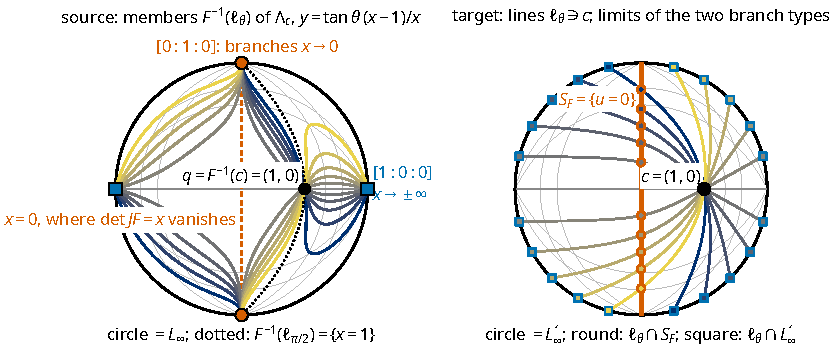
\includegraphics[width=\linewidth]{figures_jac/figJ4_dicritical_concept.pdf}
\caption{The members of a pencil $\Lambda_c$ have branches at infinity of two kinds: those that $F$ sends onto the non-properness set $S_F$, and those it sends to the line at infinity. The figure illustrates Definition~\ref{td:def:dicritical} and Proposition~\ref{td:prop:count}(b) on the map $F(x,y)=(x,xy)$. This map is not a Keller map, since $\det JF=x$; it is used only because every curve is explicit, and it is not an example of the results of this part. Here $S_F=\{u=0\}$, $c=(1,0)$ and $F^{-1}(c)=\{(1,0)\}$. Left: the members $F^{-1}(\ell_\theta)=\{y=\tan\theta\,(x-1)/x\}$ for ten directions $\theta$. Right: the lines $\ell_\theta$ through $c$. As $x\to0$ a member runs to $[0{:}1{:}0]$ and its image tends to $\ell_\theta\cap S_F=(0,-\tan\theta)$ (round markers); as $\theta$ varies these branches sweep out $S_F$. As $x\to\pm\infty$ it runs to $[1{:}0{:}0]$ and its image tends to $[1{:}\tan\theta{:}0]$ on $L'_\infty$ (square markers). Both panels use the disc model $p\mapsto p/(1+|p|)$, whose boundary circle is the line at infinity with antipodes identified; it distorts distances, not incidences. Only real points are drawn.}
\label{td:fig:dicritical}
\end{figure}

\subsection{Counting dicriticals}

The first result counts the dicriticals of $\Lambda_c$ when $c$ lies outside the
non-properness set. It uses only (F1)--(F3) and \eqref{td:eq:SF-image}.

\begin{proposition}[The count]\label{td:prop:count}
\textit{Status: grade B, proof by hand from \textnormal{(F1)--(F3)}.}
Let $F$ be a Keller map and $c \in \mathbb{A}^2 \setminus S_F$.
\begin{enumerate}[label=(\alph*),nosep]
\item The affine dicriticals of $\Lambda_c$ are exactly the $e$ exceptional curves $E_q$ of
the blow-ups at the points $q \in F^{-1}(c)$. Each has degree $1$.
\item The dicriticals at infinity are the curves at infinity $D$ of $X$ for which $G(D)$ is a
curve. For such $D$, $G(D)$ is $L'_\infty$ or a component of $\bar{S}_F$, the point $c$ does
not lie on $G(D)$, and
\begin{equation}\label{td:eq:count-degree}
m(D) = \deg\big(D \to G(D)\big) \cdot \deg G(D).
\end{equation}
\item $L'_\infty$ and every component of $\bar{S}_F$ are $G(D)$ for at least one such $D$.
So the number $N_\infty(c)$ of dicriticals at infinity satisfies
\begin{equation}\label{td:eq:count-lower}
N_\infty(c) \geq 1 + \#\{\text{components of } S_F\}.
\end{equation}
\end{enumerate}
\end{proposition}

\begin{proof}
\emph{Part (a).} Since $c \notin S_F$, the map $F$ is proper over a neighbourhood $U$ of $c$.
It is also \'{e}tale by (F1), so $F^{-1}(U) \to U$ is a finite \'{e}tale cover of degree $e$, and
the fibre $F^{-1}(c)$ consists of exactly $e$ points, at each of which $F$ is a local
isomorphism. The map $\varphi_c$ is a morphism wherever $(P - c_1, Q - c_2) \neq (0,0)$, that is,
away from $F^{-1}(c)$. A divisor whose centre is a point where $\varphi_c$ is a morphism carries
the constant value of $\varphi_c$ at that point, so it is not dicritical. Now fix
$q \in F^{-1}(c)$. Near $q$ the map $\varphi_c$ is the projection from $c$ composed with a local
isomorphism taking $q$ to $c$. After one blow-up at $q$, the exceptional curve $E_q$
parametrizes the tangent directions at $q$, and $\varphi_c|_{E_q}$ is the projectivized
differential of $F$ at $q$, an isomorphism $E_q \to \mathbb{P}^1$. So $E_q$ is dicritical of
degree $1$, and $\varphi_c$ is a morphism on a neighbourhood of $E_q$; divisors with centre on
$E_q$ are therefore not dicritical. This leaves exactly the $e$ curves $E_q$.

\emph{Part (b).} Let $D$ be a curve at infinity. Suppose first that $G(D)$ is a point $p$. By
\eqref{td:eq:SF-image}, a point of $G(X \setminus \mathbb{A}^2)$ in $\mathbb{A}^2$ lies in
$S_F$; since $c \notin S_F$, we get $p \neq c$. Then $\pi_c$ is defined at $p$, the composite
$\varphi_c = \pi_c \circ G$ takes on $D$ the single value $\pi_c(p)$, and $D$ is not dicritical.

Suppose next that $G(D)$ is a curve $C$. Either $C = L'_\infty$, or $C$ meets $\mathbb{A}^2$, and
then $C \cap \mathbb{A}^2 \subset S_F$ by \eqref{td:eq:SF-image}; being irreducible, $C$ is then a
component of $\bar{S}_F$. In both cases $c \notin C$: the affine point $c$ is not on
$L'_\infty$, and it is not on $S_F$. A projection from a point not on a plane curve $C$ restricts
to a morphism $C \to \mathbb{P}^1$ of degree $\deg C$, because a general line through $c$ meets
$C$ in $\deg C$ distinct points, none of them $c$. Composing with $D \to C$ gives
\[
m(D) = \deg(\varphi_c|_D) = \deg\big(D \to C\big) \cdot \deg\big(\pi_c|_C\big)
= \deg\big(D \to G(D)\big) \cdot \deg G(D),
\]
which is \eqref{td:eq:count-degree}. In particular $m(D) \geq 1$ and $D$ is dicritical. So the
dicriticals at infinity are exactly the curves at infinity with one-dimensional image.

\emph{Part (c).} The morphism $G$ is surjective, and $G(\mathbb{A}^2) = F(\mathbb{A}^2)$ lies in
$\mathbb{A}^2$, so $L'_\infty$ is contained in the finite union of the closed sets $G(D)$, $D$ a
curve at infinity. Being irreducible, $L'_\infty$ equals one of them. In the same way, by
\eqref{td:eq:SF-image} and (F2), each component of $S_F$ is contained in, hence equal to the affine
part of, some $G(D)$. Distinct images come from distinct curves $D$, and each such $D$ is
dicritical by part (b). Counting $L'_\infty$ and the components of $S_F$ gives
\eqref{td:eq:count-lower}.
\end{proof}

\begin{corollary}[Automorphisms]\label{td:cor:automorphisms}
\textit{Status: grade B.}
If $F$ is an automorphism, then $\Lambda_c$ has exactly two dicriticals for every $c$: one
affine, over $F^{-1}(c)$, and one at infinity, the unique curve $D$ with
$G(D) = L'_\infty$ (here $G$ is birational). Both have degree $1$.
\end{corollary}

\begin{proof}
If $F$ is an automorphism, then $e = 1$ and $S_F = \emptyset$ by (F3), so every $c$ is allowed in
Proposition~\ref{td:prop:count}. Part (a) gives exactly one affine dicritical, over the single
point $F^{-1}(c)$, of degree $1$. By part (b) a dicritical at infinity has image $L'_\infty$ or a
component of $\bar S_F = \emptyset$, so its image is $L'_\infty$, and part (c) shows that one
exists. Since $G$ is birational, exactly one curve of $X$ maps onto $L'_\infty$, with
$\deg(D \to L'_\infty) = 1$, and \eqref{td:eq:count-degree} gives $m(D) = 1 \cdot 1 = 1$.
\end{proof}

\subsection{The October 1 main theorem is false}

\begin{corollary}[The theorem as worded fails]\label{td:cor:count-fails}
\textit{Status: grade B in general; exact in the examples below.}
Every Keller map of degree at least $2$ has at least two exceptional dicriticals in
$\Lambda_0$, after a translation of the target that puts $0$ in
$F(\mathbb{A}^2) \setminus S_F$. An automorphism needs no translation. Hence the October 1
draft's theorem (``no two distinct dicritical divisors,'' with no at-infinity restriction) is
false for every Keller map of degree at least $2$. If only exceptional curves count as
divisors of the resolution, it holds exactly for affine maps, whose dicritical at infinity is
$L_\infty$ itself; if $L_\infty$ counts, it fails for them too.
\end{corollary}

\begin{proof}
Let $F$ have degree at least $2$. Translate the target so that $0 \notin S_F$ and
$0 \in F(\mathbb{A}^2)$; this is possible because $S_F$ is at most a curve and $F$ is dominant.
Then $F^{-1}(0)$ is nonempty. By Proposition~\ref{td:prop:count}(a), each point of $F^{-1}(0)$
contributes an affine dicritical of degree $1$, and by part (c) there is at least one dicritical
at infinity. That dicritical is not $L_\infty$, by Lemma~\ref{td:lem:linf} below (which needs
degree at least $2$), so it too is exceptional. That is already two exceptional dicriticals.
Example~\ref{td:ex:automorphism} exhibits both of them for an automorphism, where no
translation is needed.
\end{proof}

\begin{example}[Two dicriticals of an automorphism]\label{td:ex:automorphism}
Take
\begin{equation}\label{td:eq:auto-map}
P = x - y^2, \qquad Q = y.
\end{equation}
We compute the Jacobian bracket. The partial derivatives are
\[
P_x = 1, \qquad P_y = -2y, \qquad Q_x = 0, \qquad Q_y = 1,
\]
and substituting them into the bracket gives
\[
[P,Q] = P_x Q_y - P_y Q_x = 1 \cdot 1 - (-2y) \cdot 0 = 1 \in K^\times,
\]
so $F = (P,Q)$ is a Keller map. It is an automorphism. Solving $Q = y$ for $y$ gives $y = Q$,
and then $P = x - y^2$ gives $x = P + Q^2$; so the inverse is $(u,v) \mapsto (u + v^2, v)$, and
indeed $P + Q^2 = (x - y^2) + y^2 = x$.

\emph{The affine dicritical.} The fibre over $0$ is the single point $(0,0)$, since $Q = y = 0$
and then $P = x - y^2 = 0$ forces $x = 0$. Blow up $\mathbb{A}^2$ at the origin and use the chart
\[
x = s, \qquad y = s t,
\]
in which the exceptional curve $E$ is $\{s = 0\}$, with coordinate $t$. Substituting into $P$ and
$Q$ and factoring out $s$:
\begin{align*}
P &= s - (st)^2 = s - s^2 t^2 = s\,(1 - s t^2), \\
Q &= s t.
\end{align*}
The map $\varphi_0 = [P : Q]$ is the projection from $0$; on this chart we may cancel the common
factor $s$:
\[
\varphi_0 = [P : Q] = [\,s(1 - s t^2) : s t\,] = [\,1 - s t^2 : t\,].
\]
Setting $s = 0$ restricts it to $E$:
\[
\varphi_0|_E = [1 : t],
\]
which is non-constant in $t$, of degree $1$. Hence $E$ is dicritical of degree $1$.

\emph{The dicritical at infinity.} By Corollary~\ref{td:cor:automorphisms}, $\Lambda_0$ has
exactly one dicritical at infinity, the unique curve $D$ with $G(D) = L'_\infty$, also of degree
$1$. With the affine dicritical above, this makes two distinct dicriticals. The October 1
theorem, which forbade two distinct dicritical divisors without any at-infinity restriction, is
therefore false already for automorphisms.
\end{example}

\subsection{The corrected statement: Theorem R}

\begin{theorem}[Theorem R, the corrected main theorem; OPEN]\label{td:thm:R}
\textit{Status: open; it is not proved in this paper.}
For every Keller map $(P,Q)$, the pencil $\lambda P + \mu Q$ has at most one dicritical
divisor at infinity.
\end{theorem}

\begin{proposition}\label{td:prop:onedic}
\textit{Status: grade B.}
Let $F$ be a Keller map and $c \notin S_F$. Then $\Lambda_c$ has at most one dicritical at
infinity if and only if $F$ is an automorphism. In that case it has exactly one, of degree $1$.
\end{proposition}

\begin{proof}
If $F$ is an automorphism, Corollary~\ref{td:cor:automorphisms} gives exactly one dicritical at
infinity, of degree $1$. Conversely, suppose $\Lambda_c$ has at most one dicritical at infinity.
By Proposition~\ref{td:prop:count}(c), the number of dicriticals at infinity is at least
$1 + \#\{\text{components of } S_F\}$. So the number of components of $S_F$ is $0$, and since
$S_F$ is empty or a curve by (F2), $S_F = \emptyset$. By (F3), $F$ is an automorphism.
\end{proof}

\begin{proposition}[Theorem R is equivalent to the planar Jacobian conjecture]\label{td:prop:equiv}
\textit{Status: grade B.}
Theorem~R holds for all Keller maps if and only if the planar Jacobian conjecture holds.
\end{proposition}

\begin{proof}
If the conjecture holds, every Keller map is an automorphism, and
Corollary~\ref{td:cor:automorphisms} gives exactly one dicritical at infinity, in particular at
most one. So Theorem~R holds.

Conversely, assume Theorem~R and let $F$ be a Keller map. Pick $c \notin S_F$; such a $c$ exists
because $S_F$ is empty or a curve, never the whole target. Then $F - c$ is a Keller map, with the
same bracket, and $S_{F-c} = S_F - c$ does not contain $0$. Its pencil
$\lambda (P - c_1) + \mu (Q - c_2)$ is $\Lambda_c(F)$. Theorem~R applied to $F - c$ says that
$\Lambda_c(F)$ has at most one dicritical at infinity, and Proposition~\ref{td:prop:onedic}
(which rests on Proposition~\ref{td:prop:count} and (F3)) then makes $F$ an automorphism. Since
$F$ was arbitrary, the conjecture holds.
\end{proof}

The content of Proposition~\ref{td:prop:equiv} is known in substance, and we record its
sources. The forward direction is classical: a counterexample to JC(2) has a dicritical curve at
infinity, in Borisov's terminology a curve of type~$3$, on which the map is ramified
(Borisov~\cite[Thm.~3.1]{Borisov2011}; Borisov remarks there that the fact is well known and has
a topological proof). His argument ends in the birational case of the conjecture, which is
classical: Keller~\cite{Keller1939} treats the birational case, and
Borisov~\cite[proof of Thm.~14]{Borisov2009} gives a short direct argument through the
Abhyankar--Moh--Suzuki theorem. The description of $S_F$ as the union of the images of the
dicritical Newton--Puiseux series of $F$ is recorded by Chau~\cite[\S1, item (iii)]{Chau2007}.
Here a \emph{Newton--Puiseux series at infinity} is a finite fractional power series
$y = \sum_k a_k x^{1 - k/m} + \xi\, x^{1 - n/m}$ in $x^{-1/m}$ with a free parameter $\xi$, and it
is \emph{dicritical} when $F(x, y(x,\xi))$ tends, as $x \to \infty$, to a non-constant polynomial
function of $\xi$; we use this description only as background. Our contribution is the
formulation in terms of the pencil $\Lambda_c$. Proposition~\ref{td:prop:equiv} keeps grade B;
the attribution in this paragraph is grade C at independence level I1.

\begin{remark}
Proposition~\ref{td:prop:equiv} sets the bar for this part: a complete proof of Theorem~R would
be a proof of the conjecture. Everything that follows is measured against that bar, and no step
below is presented as reaching it.
\end{remark}

\subsection{Where a counterexample's dicriticals would sit}\label{td:sec:where}

Let $F$ be a Keller map that is not an automorphism, and let $c \notin S_F$. By (F3) and
Proposition~\ref{td:prop:count}(a), $\Lambda_c$ has $e \geq 2$ affine dicriticals. By
Proposition~\ref{td:prop:count}(b),(c) it also has at least one curve $E_\infty$ with
$G(E_\infty) = L'_\infty$, of degree $\deg(E_\infty \to L'_\infty)$, and over each component $C$
of $S_F$ at least one curve $E_S$ with $G(E_S) = C$, of degree $\deg(E_S \to C) \cdot \deg C$ by
\eqref{td:eq:count-degree}. Since $E_\infty$ always exists, Theorem~R for $\Lambda_c$ amounts to
showing that no $E_S$ exists: if there is no $E_S$, then $S_F$ has no component, so
$S_F = \emptyset$, and (F3) with Proposition~\ref{td:prop:onedic} gives exactly one dicritical
at infinity; if some $E_S$ exists, $E_\infty$ and $E_S$ are two.

The two halves of the October 1 draft, read against this picture, were as follows. The first half
claimed that no Keller map has a dicritical of degree $m \geq 2$; applied to $E_S$, this would
already exclude every counterexample whose $S_F$ has a component of degree at least $2$. The
second half claimed that there are no two dicriticals of degree $1$, which would handle the rest.
To succeed, either half must apply to $E_\infty$ and $E_S$ wherever they sit in the resolution
tree: over any point of $L_\infty$, at any depth, and after free or satellite blow-ups.
Sections~\ref{td:sec:depth01}--\ref{td:sec:bridge} record how far each half actually goes.

\section{Dicriticals at infinity of small depth}\label{td:sec:depth01}

We now take the first two steps toward Theorem~R: the line at infinity (depth $0$) and the
first blow-ups on it (depth $1$). Both turn on the same observation. The Keller condition kills
the bracket in high degree, and a vanishing bracket forces two leading parts to be proportional.
The section ends with the constant-leading-form argument, which is only a sketch and covers free
centres only. Its limits are stated where it appears. The conclusion is that every dicritical at
infinity of a non-affine Keller map has depth at least $2$.

\subsection{The line at infinity}\label{td:sec:linf}

The following lemma is in substance due to Borisov, who shows that for a counterexample to the
conjecture the strict transform of the source line at infinity is a curve of type~$2$, that is,
it is mapped to a point of the target line at infinity \cite[Prop.~15]{Borisov2009},
\cite[Cor.~3.1]{Borisov2011}. Such a curve is not dicritical, since its image is a point other
than $c$. Our statement is for an arbitrary non-affine Keller map, and we include a short
self-contained proof.

\begin{lemma}[The line at infinity]\label{td:lem:linf}
\textit{Status: grade B, proof by hand; the binary-form step is executed in
\filename{base\_point\_at\_infinity\_check.py}, check $1$, and is not in the Lean files of the
repository.}
For a non-affine Keller map, $L_\infty$ is not dicritical for any $\Lambda_c$.
\end{lemma}

The identification of Borisov's ``type~$2$'' with ``not dicritical'' made in the paragraph above
is our reading, grade C. The lemma itself keeps grade B, and we claim no novelty for it.

\begin{proof}
Let $d = \max(\deg P, \deg Q)$. A Keller map of degree $1$ is affine, so $d \geq 2$. Write $P_d$
and $Q_d$ for the homogeneous components of degree $d$ of $P$ and $Q$, setting a component to $0$
when the polynomial has smaller degree. In homogeneous coordinates $[X:Y:Z]$ with
$L_\infty = \{Z = 0\}$,
\[
P - c_1 = Z^{-d}\big(P_d(X,Y) + Z\cdot(\cdots)\big), \qquad
Q - c_2 = Z^{-d}\big(Q_d(X,Y) + Z\cdot(\cdots)\big),
\]
so the restriction of $\varphi_c$ to $L_\infty$ is $[P_d : Q_d]$, and the point $c$ plays no
part in it. We show that this ratio is constant.

\emph{Case 1: unequal degrees.} If $\deg Q < \deg P = d$, then $Q_d = 0$ and $P_d \neq 0$, so
the restriction is $[P_d : 0] = [1 : 0]$ wherever $P_d \neq 0$, hence everywhere on
$L_\infty$. It is constant, and $L_\infty$ is not dicritical. The case $\deg P < \deg Q$ gives the
constant $[0 : 1]$ in the same way.

\emph{Case 2: equal degrees.} Suppose $\deg P = \deg Q = d$, so $P_d \neq 0$ and $Q_d \neq 0$.
Each partial derivative of $P$ has top component the corresponding partial derivative of $P_d$,
of degree $d-1$, and likewise for $Q$. The products in the bracket therefore have degree at most
$2d - 2$, and their components of degree exactly $2d - 2$ come only from the top components:
\[
[P,Q]_{2d-2} = (P_d)_x (Q_d)_y - (P_d)_y (Q_d)_x = [P_d, Q_d].
\]
Since $2d - 2 \geq 2 > 0$ and $[P,Q]$ is a constant, this component vanishes:
\begin{equation}\label{td:eq:top-bracket}
[P,Q]_{2d-2} = [P_d, Q_d] = 0.
\end{equation}
So it suffices to prove the following binary-form lemma.

\begin{lemma}[Proportionality of binary forms with vanishing bracket]\label{td:lem:binary}
Let $f, g$ be binary forms (homogeneous polynomials in two variables) of the same degree
$\geq 1$, and suppose $g \neq 0$. If $[f,g] = 0$, then $f = r g$ for some constant $r \in K$.
\end{lemma}

The hypothesis $g \neq 0$ was missing in the earlier version, and the statement without it is
false: $f = x$, $g = 0$ have $[f,g] = 0$, but $x$ is not a multiple of $0$. In the use of the
lemma in Case 2 above, $g = Q_d \neq 0$, and in its later use in the proof of
Proposition~\ref{td:prop:P2}, $g = Q_D \neq 0$; so the missing hypothesis is always satisfied
and nothing downstream changes.

\begin{proof}[Proof of Lemma~\ref{td:lem:binary}]
Work in the field $K(x,y)$ and set $h = f/g$, which makes sense because $g \neq 0$. As a quotient
of two forms of the same degree, $h$ is homogeneous of degree $0$: $h(tx, ty) = h(x,y)$.
Differentiating this identity in $t$ at $t = 1$ gives Euler's relation
\begin{equation}\label{td:eq:euler-h}
x h_x + y h_y = 0.
\end{equation}
Next, by the quotient rule and $[g,g] = 0$,
\[
[h, g] = \frac{[f,g]}{g} - \frac{f\,[g,g]}{g^2} = \frac{[f,g]}{g} = 0,
\]
which, written out, is
\begin{equation}\label{td:eq:bracket-hg}
g_y\, h_x - g_x\, h_y = 0.
\end{equation}
Read \eqref{td:eq:euler-h} and \eqref{td:eq:bracket-hg} as a linear system in the unknowns
$h_x, h_y$ over $K(x,y)$. Its determinant is
\[
\det\begin{pmatrix} x & y \\ g_y & -g_x \end{pmatrix} = -(x g_x + y g_y) = -(\deg g)\, g,
\]
by Euler's relation for the form $g$. This is nonzero, because $\deg g \geq 1$, the
characteristic is $0$ and $g \neq 0$. So the only solution is $h_x = h_y = 0$. In characteristic
$0$ a rational function with both partial derivatives zero is a constant, so $h = r \in K$ and
$f = r g$.
\end{proof}

We return to Case 2. Lemma~\ref{td:lem:binary} with $f = P_d$ and $g = Q_d \neq 0$ gives
$P_d = r Q_d$, so $\varphi_c|_{L_\infty} = [r : 1]$ is constant, and $L_\infty$ is not dicritical.
\end{proof}

The binary-form step, with the hypothesis $g \neq 0$, has since been checked by the Lean kernel in
a separate Lean project of the November 2026 campaign, outside the repository. There it appears as
\texttt{binary\_\allowbreak{}form\_\allowbreak{}proportional}, together with the counterexample
\texttt{binary\_\allowbreak{}form\_\allowbreak{}needs\_\allowbreak{}g\_\allowbreak{}ne\_\allowbreak{}zero} to the statement without $g \neq 0$. This leaves the grade of
Lemma~\ref{td:lem:linf} at B, and Part~\ref{rp:part} reports the campaign work.

\subsection{First blow-ups at infinity}\label{td:sec:e1lemma}

Next we blow up once at a point of $L_\infty$. The same mechanism applies, with the $x$-degree
in place of the total degree and a Wronskian in place of the bracket of the two forms. The lemma
overlaps Borisov's study of the first blow-ups in a resolution of a counterexample
\cite[Props.~3.2--3.3 and Thm.~3.3]{Borisov2011}; we have not checked whether his statements
are exactly equivalent to ours.

\begin{lemma}[First blow-ups at infinity]\label{td:lem:e1}
\textit{Status: algebra grade A, in \filename{lean/TwoDicritical/E1Keller.lean}
(\texttt{e1\_\allowbreak{}lead\_\allowbreak{}proportional}, \texttt{jac2\_\allowbreak{}eq\_\allowbreak{}zero\_\allowbreak{}of\_\allowbreak{}natDegree\_\allowbreak{}zero}); chart step
grade B, executed in \filename{lean/check\_e1\_index.py}, check $5$, not Lean-formalized.}
For a Keller map, the exceptional curve of the blow-up at any point of $L_\infty$ is not
dicritical. This holds for every degree $m$, not only for $m = 2$.
\end{lemma}

\begin{proof}
A linear change of coordinates preserves the Keller condition, because the bracket is multiplied by
the constant determinant of the change. So we may assume the point of $L_\infty$ is $[1:0:0]$.
In the chart of the blow-up that we use,
\begin{equation}\label{td:eq:e1-chart}
x = \frac{1}{s_1 t_1}, \qquad y = \frac{1}{t_1}, \qquad E_1 = \{s_1 = 0\},
\end{equation}
obtained from the affine coordinates $s = y/x$, $t = 1/x$ at $[1:0:0]$ by $s = s_1$,
$t = s_1 t_1$. Then $t_1$ is a coordinate on $E_1$. The proof has three steps: the restriction
formula, the Wronskian computation and the degenerate case.

\emph{Step 1: the restriction formula.} Suppose $P$ and $Q$ have the same $x$-degree $n \geq 1$,
with $x^n$-coefficients $A, D \in K[y]$:
\begin{equation}\label{td:eq:lead-expansion}
P = A(y)\, x^n + (\text{terms of $x$-degree} < n), \qquad
Q = D(y)\, x^n + (\text{terms of $x$-degree} < n).
\end{equation}
In the chart \eqref{td:eq:e1-chart}, a monomial $x^i y^j$ becomes
$s_1^{-i} t_1^{-i-j}$. So $x$-degree $i$ means a pole of order exactly $i$ along $E_1$, and
\[
s_1^n P = t_1^{-n} A(1/t_1) + s_1 \cdot (\cdots), \qquad
s_1^n Q = t_1^{-n} D(1/t_1) + s_1 \cdot (\cdots).
\]
Setting $s_1 = 0$ in the ratio, the factor $t_1^{-n}$ cancels, and
\begin{equation}\label{td:eq:e1-restriction}
\frac{P}{Q}\bigg|_{E_1} = \frac{A(1/t_1)}{D(1/t_1)}.
\end{equation}
The constant $c$ again plays no part, since $c_1$ and $c_2$ have $x$-degree $0 < n$. If instead
$\deg_x P > \deg_x Q$, the same computation gives the constant $\infty$, and
$\deg_x P < \deg_x Q$ gives the constant $0$. In both of these cases $E_1$ is not dicritical, so
only the case of equal $x$-degree remains.

\emph{Step 2: the Wronskian computation.} Differentiate \eqref{td:eq:lead-expansion} term by
term and keep the top $x$-degree:
\begin{align*}
P_x &= n A(y)\, x^{n-1} + (\text{$x$-degree} < n-1), &
P_y &= A'(y)\, x^{n} + (\text{$x$-degree} < n), \\
Q_x &= n D(y)\, x^{n-1} + (\text{$x$-degree} < n-1), &
Q_y &= D'(y)\, x^{n} + (\text{$x$-degree} < n).
\end{align*}
The products $P_x Q_y$ and $P_y Q_x$ both have $x$-degree at most $2n - 1$, with
$x^{2n-1}$-coefficients $nAD'$ and $nA'D$. Lowering the $x$-degree of either factor lowers the
total, so no other product reaches $x^{2n-1}$. Therefore
\begin{equation}\label{td:eq:wronskian-coeff}
[P,Q]_{x^{2n-1}} = n\,\big(A D' - A' D\big).
\end{equation}
Since $[P,Q]$ is a constant and $2n - 1 \geq 1$, this coefficient vanishes, and since $n \geq 1$
in characteristic $0$,
\[
A D' - A' D = 0.
\]
This is the vanishing of the Wronskian of $A$ and $D$. Here $D \neq 0$, because $\deg_x Q = n$.
So
\[
\left(\frac{A}{D}\right)' = \frac{A' D - A D'}{D^2} = 0,
\]
and $A/D$ is a constant $r$; that is, $A = rD$. This is the Lean lemma
\texttt{e1\_\allowbreak{}lead\_\allowbreak{}proportional}. Substituting into \eqref{td:eq:e1-restriction},
\[
\frac{P}{Q}\bigg|_{E_1} = \frac{r D(1/t_1)}{D(1/t_1)} = r,
\]
a constant. So $E_1$ is not dicritical in the case of equal $x$-degree either.

\emph{Step 3: the degenerate case.} If both $x$-degrees are $0$, then $P, Q \in K[y]$, so
$P_x = Q_x = 0$ and $[P,Q] = 0$. This contradicts the Keller condition (Lean lemma
\filename{jac2\_eq\_zero\_of\_natDegree\_zero}), so this case does not occur.

The reduction to $[1:0:0]$ at the start covers every point of $L_\infty$.
\end{proof}

\begin{corollary}[Depth at least $2$]\label{td:cor:depth2}
\textit{Status: grade B; it follows from Lemmas~\ref{td:lem:linf} and~\ref{td:lem:e1}.}
Every dicritical at infinity of a non-affine Keller map has depth at least $2$.
\end{corollary}

\begin{proof}
The only curve of depth $0$ is $L_\infty$, which Lemma~\ref{td:lem:linf} excludes for non-affine
maps. The curves of depth $1$ are the exceptional curves of blow-ups at points of $L_\infty$, and
Lemma~\ref{td:lem:e1} excludes these. What remains has depth at least $2$.
\end{proof}

\subsection{The constant-leading-form argument: a sketch for free centers only}\label{td:sec:constant-form}

Beyond depth $1$ we have only a sketch. We record it because it identifies the mechanism that a
proof of obligation O3 would have to extend, and because the October 1 draft relied on it.

\begin{proposition}[Constant leading form, proof sketch]\label{td:prop:constant-form}
\textit{Status: grade C, proof sketch; free centers only. This is not a proof for satellite
chains, or for depth $\geq 2$ in general (obligation O3).}
Suppose $E_k$, $k \geq 2$, is dicritical of order $m \geq 1$ for the pencil, and reached by free
centres only. Then, after the standard normalization, the leading coefficient satisfies
$\deg_{u'} U(u',0) = 0$.
\end{proposition}

\begin{proof}[Proof sketch]
Let $(u', v')$ be local coordinates in which $E_k = \{v' = 0\}$. For $S \in K[x,y]$ of degree $d$,
write the pullback as
\begin{equation}\label{td:eq:pullback}
S = {v'}^{-\nu}\,U(u',v')\cdot(\text{monomial in }u'),
\end{equation}
where $\nu = \nu_{E_k}(S)$ is the order of the pole and $U$ does not vanish at the centre. The
dicritical condition of order $m$ asks that the restriction of the pencil have $u'$-degree $m$.

We follow $U$ through the blow-ups, one at a time. At a \emph{free} centre $u_0 \neq 0$, the
local coordinate $u'$ is a nonzero constant at the centre. Substituting the centre into the
blow-up chart multiplies the leading coefficient by the nonzero constant $u_0^{-2}$. If the
leading term was $c\,{u'}^{j}$, it becomes $c\, u_0^{-2}\, {u''}^{j}$ in the new coordinate
$u''$, with the same exponent. No new dependence on $u'$ appears, because $u_0$ is a constant
and not a function of $u'$. Along a chain of free centres the leading coefficient is therefore
multiplied by a nonzero constant at each step, and its $u'$-degree does not change. A direct
computation in the normalized chart then gives $u'$-degree $0$ for $U(u',0)$. The degree count is
checked in \filename{general\_constant\_form.py} (\S\ref{td:sec:correspondence}).

\emph{Where the sketch stops.} Each step uses $u_0 \neq 0$. At a satellite centre, which lies on
another component of the total transform, the relevant coordinate vanishes at the centre. The
factor is then no longer a nonzero constant, and the degree count above fails. So the sketch covers
free chains only. It does not show that no $E_k$, $k \geq 2$, is dicritical of order $m \geq 2$
in general, and we do not claim that it does; the general statement at depth $\geq 2$ is
obligation O3 in \S\ref{td:sec:open}. The middle divisor $E_2$ and the leaves $E_3$, $E_4$ are
checked separately, as fixed instances rather than the general argument, in
\filename{middle\_e2.py}, \filename{leaf\_e3.py} and \filename{leaf\_e4.py}.
\end{proof}

\begin{remark}
In the October 1 draft, Proposition~\ref{td:prop:constant-form} was followed by a corollary
claiming that no $E_k$, $k \geq 2$, is dicritical of order $m \geq 2$ for any Keller map, and
that corollary was used to close the $m \geq 2$ half of the main theorem. The inference is
withdrawn: a sketch for free centres does not yield the general corollary, and this revision
does not claim it anywhere.
\end{remark}

\section{The first exceptional divisor: a false obstruction and its correction}\label{td:sec:e1}

The October 1 draft also contained a direct obstruction at $E_1$, which is false. We show where
its proof goes wrong and give a counterexample in full. The true statement, which the draft was
aiming at, is Lemma~\ref{td:lem:e1}: first blow-ups at infinity are never dicritical for a Keller
map, for every degree $m$. That lemma has wider scope than the draft's claim, since it covers every
$m$ and not only $m = 2$, and it says less about $E_1$ itself: it makes no claim about a
hypothetical ``$m = 2$ open subset,'' which, as the counterexample shows, contains Keller pairs.

\subsection{What the October 1 draft claimed}

In substance, the draft's $E_1$ degree obstruction read as follows. Let $P, Q$ lie in the
``$E_1$, $m = 2$ open subset,'' meaning $\nu_{E_1} = -2$ and both pencil restrictions have exact
degree $2$; then $[P,Q]$ is never a nonzero constant. The proof ran: every monomial $x^J y^K$
allowed by the order condition $\nu_{E_1} \geq -2$ has $J + K \geq 2$; hence $P_x, P_y, Q_x, Q_y$
have no constant term; hence every term of $[P,Q]$ has total degree at least $2$, and $[P,Q]$
cannot be a nonzero constant. Each step after the first is correct arithmetic. The first is false.

\subsection{The order condition, computed correctly}

\begin{lemma}[The $E_1$ order condition]\label{td:lem:e1-order}
In the $E_1$ chart \eqref{td:eq:e1-chart},
\begin{equation}\label{td:eq:e1-valuation}
\nu_{E_1}(x^i y^j) = -i.
\end{equation}
Consequently $\nu_{E_1}(x^i y^j) \geq -2$ if and only if $i \leq 2$, that is, if and only if the
$x$-degree is at most $2$. The condition says nothing about the total degree $i + j$.
\end{lemma}

\begin{proof}
By \eqref{td:eq:e1-chart}, $x = s_1^{-1} t_1^{-1}$ and $y = t_1^{-1}$, so along $E_1 = \{s_1 = 0\}$
the function $x$ has a pole of order $1$ and $y$ has neither zero nor pole. This is the valuation
used in \filename{lean/check\_e1\_index.py} and \filename{lean/TwoDicritical/E1Keller.lean}. Hence
\[
\nu_{E_1}(x^i y^j) = i \cdot \nu_{E_1}(x) + j \cdot \nu_{E_1}(y) = i \cdot (-1) + j \cdot 0 = -i,
\]
and $-i \geq -2$ is $i \leq 2$. The condition bounds the $x$-degree and nothing else. In particular
the monomial $y$, with $i = 0$ and $j = 1$, has $\nu_{E_1}(y) = 0 \geq -2$ and total degree $1$.
So the draft's claim that every allowed monomial has $J + K \geq 2$ fails as soon as the valuation
is written out.
\end{proof}

\subsection{How the mix-up happened}

The error is a mix-up of indices, identified in the analysis accompanying the Lean files
(\filename{lean/README.md}, item 2). The computation \filename{e1\_solitary.py} indexes its
unknowns $p[J,K]$ by the homogeneous monomial $X^{d-J-K} Y^J Z^K$, that is, by the affine
monomial $x^{d-J-K} y^J$. The draft's proof, the script \filename{e1\_keller\_search.py} and the
Lean file \filename{lean/TwoDicritical/E1Obstruction.lean} read $p[J,K]$ as $x^J y^K$ instead.
Under that reading, the condition on the indices turns into a condition on the total degree
$J + K$, and the draft concluded that every allowed monomial has total degree at least $2$. At
$d = 4$ both index sets have $12$ monomials, so the counts agreed and the mix-up went unnoticed.
The $12$-dimensional span at $d = 4$ is real, but it is spanned by monomials of $x$-degree at most
$2$, not by monomials of total degree at least $2$. The file
\filename{lean/TwoDicritical/E1Obstruction.lean} proves a true lemma about the misread set
(\texttt{not\_\allowbreak{}keller\_\allowbreak{}of\_\allowbreak{}noLowTerms}: if every monomial of $P$ and $Q$ has total degree at least
$2$, then $[P,Q]$ has no constant term), but that set is not the $E_1$ condition, so the lemma says
nothing about $E_1$.

\subsection{The counterexample, computed in full}

\begin{example}[A Keller pair in the draft's $E_1$ open subset]\label{td:ex:e1-counter}
\textit{Status: grade A in Lean (\filename{lean/TwoDicritical/E1Keller.lean},
\texttt{thm\_\allowbreak{}e1\_\allowbreak{}false}); the computation below is exact.}
Set
\begin{equation}\label{td:eq:e1-counter}
P = (x + y^2)^2 + y, \qquad Q = P + x + y^2.
\end{equation}
Expanding,
\[
P = x^2 + 2 x y^2 + y^4 + y,
\]
with partial derivatives
\begin{align}
P_x &= 2x + 2y^2 = 2\,(x + y^2), \\
P_y &= 4x y + 4y^3 + 1 = 4y\,(x + y^2) + 1.
\end{align}
Since $Q = P + x + y^2$ and $[P,P] = 0$, bilinearity gives
\[
[P,Q] = [P, x] + [P, y^2].
\]
The function $x$ has partial derivatives $1$ and $0$, so
\[
[P,x] = P_x \cdot 0 - P_y \cdot 1 = -P_y = -\big(4y(x+y^2) + 1\big).
\]
The function $y^2$ has partial derivatives $0$ and $2y$, so
\[
[P, y^2] = P_x \cdot 2y - P_y \cdot 0 = 2y P_x = 4y(x+y^2).
\]
Adding, the terms $4y(x+y^2)$ cancel:
\begin{equation}\label{td:eq:e1-bracket}
[P,Q] = -\big(4y(x+y^2) + 1\big) + 4y(x+y^2) = -1 \in K^\times.
\end{equation}
So $(P,Q)$ is a Keller pair.

It lies in the draft's $E_1$, $m = 2$ open subset at $d = 4$. Its $x$-degree is $2$, from the
term $x^2$, so $\nu_{E_1}(P) = \nu_{E_1}(Q) = -2$ by Lemma~\ref{td:lem:e1-order}, and each pencil
restriction is the function $C(t_1) = t_1^2$, of exact degree $2$. This membership is what
\texttt{thm\_\allowbreak{}e1\_\allowbreak{}false} in \filename{lean/TwoDicritical/E1Keller.lean} formalizes, the open subset
being \texttt{E1Open4} there. Yet $[P,Q] = -1$, which contradicts the draft's theorem.

Two further observations locate the failure. First, $P$ contains the monomial $y$, of total degree
$1$, so the claimed lower bound $J + K \geq 2$ fails for a monomial that is actually present.
Second, both $P$ and $Q$ have $x^2$-coefficient $A = D = 1$, so by \eqref{td:eq:e1-restriction}
the ratio $P/Q$ restricts to $1$ on $E_1$. Thus $E_1$ is not dicritical for this pair at all, and
the draft's open subset does not even capture an $m = 2$ dicritical.
\end{example}

\begin{remark}[Withdrawn theorem]
The draft's $E_1$ degree obstruction theorem and its corollary (``no dicritical of order
$m \geq 2$ exists for any Keller map'') are both withdrawn. The corollary rested on the false
theorem for $E_1$ and on the free-only sketch of Proposition~\ref{td:prop:constant-form} for
$E_k$, $k \geq 2$, and neither supports it as stated.
\end{remark}

\subsection{The corrected \texorpdfstring{$E_1$}{E1} statement}

The conclusion the draft wanted, that the first blow-up is never dicritical for a Keller map, is
true. It is Lemma~\ref{td:lem:e1}, proved for every degree $m$. In one line: when the $x$-degrees
agree, $P/Q$ restricts to $A(1/t_1)/D(1/t_1)$ on $E_1$, and when they differ it restricts to $0$
or $\infty$; the Keller condition kills the $x^{2n-1}$-coefficient
\eqref{td:eq:wronskian-coeff}, hence the Wronskian $AD' - A'D$, hence $A = rD$, and the
restriction is the constant $r$. The algebra is grade A in Lean. The chart step is executed and not
formalized (obligation O5). The corrected proof uses no $m = 2$ open subset and no argument about
total degree.

\section{The \texorpdfstring{$m=1$}{m=1} bridge, under its premises}\label{td:sec:bridge}

We turn to the second half of the October 1 draft, two dicriticals of degree $m = 1$. The
draft's argument is linear algebra: a Vandermonde determinant and a block-rank lemma. That
algebra is sound, apart from one weight treated below, but what it proves is the collapse of a
system of equations. Whether that system is the system of two geometric $m = 1$ dicriticals
depends on two premises, (P1) and (P2). Premise (P2) was obligation O2 when this part was
first written. It was settled for Keller maps on November 11, 2026
(Proposition~\ref{td:prop:P2}, grade B, I1), so for a Keller map only (P1) remains. The theorem
of this section is still a theorem about equations under premises, not an unconditional geometric statement, and its consequences are stated with the
premises attached.

\subsection{The chart and the two premises}

Over the point $[1:0:0]$ of $L_\infty$, the second exceptional curve $E_2$ carries the
coordinate $w_2 = x/y^2$. At a point $w_2 = a$ of $E_2$ we use the chart
\begin{equation}\label{td:eq:bridge-chart}
x = \frac{1}{b^2 (a + \tilde{a} b)}, \qquad y = \frac{1}{b\,(a + \tilde{a} b)},
\end{equation}
in which $x/y^2 = a + \tilde{a} b$ and the curve $b = 0$ lies over the point $a$. For a polynomial
$S$ of degree at most $d$ with homogenization $S^h(X,Y,Z)$, substituting \eqref{td:eq:bridge-chart}
gives
\[
S = \frac{S^h\big(1, b, b^2(a + \tilde{a} b)\big)}{\big(b^2(a + \tilde{a} b)\big)^{d}},
\]
so the pole order of $S$ along $b = 0$ is $2d - \operatorname{ord}_b S^h(1, b, b^2(a+\tilde a b))$.
The two centres $a_3 \neq a_4$ of the bridge are points of this $E_2$. The \emph{bridge equations}
of the next subsection rest on two premises.
\begin{enumerate}[label=(P\arabic*),leftmargin=*]
\item The two dicriticals lie over two distinct \emph{free} points of this $E_2$.
\item Every member of the pencil has pole order at most $1$ on them.
\end{enumerate}
Premise (P1) is part of the geometric reading of the equations: \eqref{td:eq:bridge-chart} is the
chart at a free point of $E_2$, and the argument takes place in that chart. For arbitrary
polynomials, premise (P2) is not a consequence of our definitions. We defined $m$ as
the degree of $\varphi_c|_E$, and degree $1$ does not force pole order $1$
(\filename{lean/check\_satellite.py}, check $7$). For Keller maps it is a consequence of (P1), by
Proposition~\ref{td:prop:P2} below. By the formula above, (P2) says that
$\operatorname{ord}_b S^h(1,b,b^2(a+\tilde a b)) \geq 2d - 1$. Deriving (P2) from the definition of
$m$, or giving a separate argument for higher pole order, was obligation O2 in
\S\ref{td:sec:open}; Proposition~\ref{td:prop:P2} discharges it for Keller maps. Every statement
below that needs (P2) says so.

\subsection{Premise (P2) for Keller maps}\label{td:sec:P2}

For a Keller map, premise (P2) follows from (P1). We give the proof here; it was found on
November 11, 2026, after the first version of this part, and it discharges obligation O2.

Fix $a \neq 0$ and put $u = x - a y^2$, $v = y$. The map $\tau(u,v) = (u + a v^2, v)$ is a
polynomial automorphism with Jacobian determinant $1$, so for polynomials $P, Q$ the composites
$P' = P \circ \tau$ and $Q' = Q \circ \tau$ satisfy $[P', Q']_{(u,v)} = [P,Q] \circ \tau$. Write
$\deg_{(u,v)}$ for the total degree in $u$ and $v$. In the chart \eqref{td:eq:bridge-chart}, with
$w = a + \tilde a b$,
\[
u = \frac{1}{b^2 w} - \frac{a}{b^2 w^2} = \frac{w - a}{b^2 w^2} = \frac{\tilde a}{b\, w^2},
\qquad v = \frac{1}{b\, w},
\qquad\text{so}\qquad
u^j v^k = \tilde a^{\,j}\, w^{-2j-k}\, b^{-(j+k)} .
\]
We read $\tilde a$ as an indeterminate, as in the setup of the bridge equations below. The
monomials $u^j v^{D-j}$ of a fixed $(u,v)$-degree $D$ then carry distinct powers $\tilde a^{\,j}$,
so their contributions to $b^{-D}$ cannot cancel, and a polynomial $S$ with
$\deg_{(u,v)} S = D \geq 1$ has pole order exactly $D$ along $b = 0$. If
$S_D = \sum_j s_j u^j v^{D-j}$ is the top homogeneous part of $S$ in $(u,v)$, then at $b = 0$,
where $w = a$,
\begin{equation}\label{td:eq:P2-restriction}
b^D S\big|_{b=0} = \sum_j s_j\, \tilde a^{\,j} a^{-j-D} = a^{-D}\, S_D(\tilde a/a,\, 1).
\end{equation}

\begin{proposition}[Premise (P2) for Keller maps]\label{td:prop:P2}
\textit{Status: grade B, independence I1. Proof by hand, November 11, 2026. The valuation formula
and the degree count of Step~4 were checked symbolically in SymPy~1.14.0, the valuation by two
independent methods (script \filename{phase1\_p2\_check.py}, exit code $0$; re-run on November 25,
2026 with the same result). The script is not part of the archive of \S\ref{td:sec:archive}.
Not formalized in Lean.}
Let $F = (P,Q)$ be a Keller map, let $a \neq 0$, and let $E_a$ be the curve $b = 0$ of the chart
\eqref{td:eq:bridge-chart}, which lies over the free point $w_2 = a$ of $E_2$. If $E_a$ is
dicritical for $\Lambda_c$ for some $c$, then every member of $\Lambda_c$ has pole order exactly
$1$ on $E_a$, and $m(E_a) = 1$. In particular (P2) holds for every dicritical over a free point
of $E_2$.
\end{proposition}

\begin{proof}
Let $D_P = \deg_{(u,v)} P'$ and $D_Q = \deg_{(u,v)} Q'$, and let $P_D$, $Q_D$ denote top
homogeneous parts. The map $\varphi_c = [P - c_1 : Q - c_2]$ does not change if we compose with
$\tau$, and subtracting a constant does not change a top part of positive degree.

\emph{Step 1: $D_P = D_Q$.} If $D_P > D_Q$, then $(P - c_1)/(Q - c_2)$ has a pole along $E_a$ and
$\varphi_c|_{E_a}$ is the constant $[1:0]$; if $D_P < D_Q$, it is the constant $[0:1]$. Either way
$E_a$ is not dicritical. So $D_P = D_Q =: D$, and $D \geq 1$, since otherwise $P$ and $Q$ would
both be constant.

\emph{Step 2: $P_D$ and $Q_D$ are linearly independent.} By \eqref{td:eq:P2-restriction},
$\varphi_c|_{E_a} = [P_D(t,1) : Q_D(t,1)]$ with $t = \tilde a/a$. A binary form of degree $D$ is
determined by its value at $(t,1)$, so this map is constant exactly when $P_D = r\, Q_D$ for a
constant $r$. Since $E_a$ is dicritical, $P_D$ and $Q_D$ are independent.

\emph{Step 3: every member has pole order $D$.} A member of $\Lambda_c$ is
$S = \lambda (P - c_1) + \mu (Q - c_2)$ with $(\lambda, \mu) \neq (0,0)$. Its top part
$\lambda P_D + \mu Q_D$ is nonzero by Step~2, so $\deg_{(u,v)} S = D$ and $S$ has pole order $D$
on $E_a$.

\emph{Step 4: $D = 1$.} The bracket $[P', Q']_{(u,v)}$ is a nonzero constant. Write
$P' = P_D + P_{<D}$ and $Q' = Q_D + Q_{<D}$. Each partial derivative lowers degree by one, so
$[P_D, Q_D]$ is homogeneous of degree $2D - 2$ or zero, and the remaining terms of the bracket
have degree at most $2D - 3$. Hence $[P_D, Q_D]$ is the component of degree $2D - 2$ of a constant.
If $D \geq 2$, then $2D - 2 \geq 2$, so $[P_D, Q_D] = 0$, and Lemma~\ref{td:lem:binary}, applied
with $g = Q_D \neq 0$, gives $P_D = r\, Q_D$, against Step~2. So $D = 1$.

By Step~3 every member of $\Lambda_c$ has pole order $1$ on $E_a$. The map
$[P_1(t,1) : Q_1(t,1)]$ is a ratio of two independent polynomials of degree at most $1$ in $t$,
so it has degree $1$, and $m(E_a) = 1$.
\end{proof}

The Keller condition is used only in Step~4, and it cannot be dropped. Check $7$ of
\filename{lean/check\_satellite.py} uses $P_7 = (x - a_4 y^2)\, y + 1$ and $Q_7 = y^2 + 1$. In the
coordinates $(u,v)$ at $a = a_4$ these are $uv + 1$ and $v^2 + 1$: their top parts $uv$ and $v^2$
are independent of degree $2$, the dicritical has degree $1$ and pole order $2$, and
$[P_7, Q_7] = y \cdot 2y - (x - 3a_4 y^2) \cdot 0 = 2y^2$, so the pair is not Keller.

\subsection{Setup of the equations}

Write $S = \sum p_{JK}\, x^J y^K$ with $J + K \leq d$. The homogeneous monomial of $x^J y^K$ is
$X^J Y^K Z^{d-J-K}$, so at a centre $a$ the numerator above is
\begin{equation}\label{td:eq:bridge-pullback}
S_a(b) = \sum_{J,K} p_{JK}\,(a + \tilde{a} b)^{d-J-K}\, b^{2d-2J-K}.
\end{equation}
Indeed, $X^J Y^K Z^{d-J-K}$ at $(1, b, b^2(a+\tilde a b))$ is
$b^K \cdot b^{2(d-J-K)} (a+\tilde a b)^{d-J-K} = (a+\tilde a b)^{d-J-K} b^{2d-2J-K}$. Under (P2),
the $m = 1$ condition at the centre $a$ is $\operatorname{ord}_b S_a \geq 2d - 1$: the coefficients of
$b^0, \dots, b^{2d-2}$ vanish. As in the October 1 draft, we read $\tilde a$ as an indeterminate, so
that each coefficient of $\tilde a^i b^t$ with $t \leq 2d - 2$ vanishes separately. This reading
belongs to the geometric premises, and it is stated, not derived, in the Lean files.

Expand by the binomial theorem:
\[
(a + \tilde{a} b)^{e} = \sum_{i \geq 0} \binom{e}{i} a^{e - i}\, \tilde{a}^{\,i}\, b^i .
\]
The \emph{weight} of $x^J y^K$ is $W = 2J + K$. A monomial of weight $W$ contributes to
$\tilde a^i b^t$ exactly when $t = 2d - W + i$. So the coefficient of $\tilde a^i b^t$ involves only
the monomials of the single weight $W = 2d - t + i$, and the condition $t \leq 2d - 2$ becomes
$i \leq W - 2$. For fixed $W$, the monomials of weight $W$ with $J + K \leq d$ are
$(J, W - 2J)$ with $\max(0, W - d) \leq J \leq \lfloor W/2 \rfloor$. List them as $(J_k, K_k)$,
$k = 1, \dots, n$, with $J_k$ strictly decreasing, so that
\[
n = n(W) = \lfloor W/2 \rfloor + 1 - \max(0, W - d),
\]
and put
\begin{equation}\label{td:eq:ek-def}
e_k = d - J_k - K_k = d - W + J_k .
\end{equation}
For $k < l$ we have $e_k - e_l = J_k - J_l > 0$, so the $e_k$ are distinct. The \emph{bridge
equations} of weight $W$ at the centre $a$ are
\begin{equation}\label{td:eq:block}
\sum_{k=1}^n p_{J_k K_k}\binom{e_k}{i} a^{e_k-i} = 0, \qquad 0 \leq i \leq W - 2, \quad
a \in \{a_3, a_4\}.
\end{equation}
Each equation contains the variables of one weight only. The system is block-diagonal in $W$, and
the blocks can be solved independently. The descending induction of the October 1 draft is not
needed.

\begin{theorem}[Bridge collapse, under (P1) and (P2)]\label{td:thm:bridge}
\textit{Status: equations grade A, in \filename{lean/TwoDicritical/BridgeCollapse.lean}
(\texttt{bridge\_\allowbreak{}collapse}, \texttt{bridge\_\allowbreak{}jacobian\_\allowbreak{}eq\_\allowbreak{}zero}); geometric reading grade B,
executed in \filename{lean/check\_satellite.py}.}
For arbitrary distinct nonzero $a_3, a_4$ and arbitrary $d \geq 2$, the simultaneous conditions
$\operatorname{ord}_b(S) \geq 2d - 1$ at both centres, in the form \eqref{td:eq:block}, force
$p_{JK} = 0$ whenever $2J + K \geq 2$, in particular whenever $J \geq 1$. The nullspace is exactly
$\operatorname{span}\{1, y\}$.
\end{theorem}

It follows that every $P, Q$ in the span is a function of $y$ alone, so $[P,Q] \equiv 0$, and the
system of equations contains no Keller pair (\texttt{bridge\_\allowbreak{}jacobian\_\allowbreak{}eq\_\allowbreak{}zero}). Whether this rules
out two geometric $m = 1$ dicriticals depends on (P1) and (P2); see \S\ref{td:sec:bridge-scope}.

\subsection{The block-rank lemma}

\begin{lemma}[Block full rank]\label{td:lem:block-rank}
Let $e_1, \dots, e_n$ be distinct nonnegative integers, $a \neq 0$, and $m \geq n$. The
$m \times n$ matrix with entries $\binom{e_k}{i} a^{e_k-i}$, $0 \leq i \leq m - 1$, has rank $n$.
\end{lemma}

The earlier version stated the lemma for the $2m \times n$ matrix of both centres and scaled column
$k$ by $a^{e_k}$, which cannot be done for two different values of $a$ at once. A single centre
suffices, and that is the form proved in Lean (\texttt{choose\_\allowbreak{}det\_\allowbreak{}ne\_\allowbreak{}zero} in
\filename{lean/TwoDicritical/BlockRank.lean}).

\begin{proof}
We reduce the matrix in three steps, each preserving rank.

\emph{Step 1: scale rows and columns.} Multiply row $i$ by $a^{i}$ and column $k$ by $a^{-e_k}$.
Both factors are nonzero because $a \neq 0$, so the rank does not change. The entry in row $i$,
column $k$ becomes $\binom{e_k}{i}$. Since $m \geq n$, it suffices to show that the leading
$n \times n$ block
\[
B_n := \left(\binom{e_k}{i}\right)_{0 \leq i \leq n-1,\ 1 \leq k \leq n}
\]
is nonsingular. Write $V_n := \bigl(e_k^{\,i}\bigr)_{0 \leq i \leq n-1,\ 1 \leq k \leq n}$ for the
Vandermonde matrix of $e_1, \dots, e_n$, and $D_n := \operatorname{diag}(0!, 1!, \dots, (n-1)!)$.

\emph{Step 2: triangularize by row operations.} For fixed $i$, $\binom{e}{i}$ is a polynomial in
$e$ of exact degree $i$ with leading coefficient $1/i!$:
\[
\binom{e}{i} = \frac{e (e-1) \cdots (e - i + 1)}{i!}
= \frac{1}{i!} e^i + (\text{terms of degree} < i \text{ in } e).
\]
So row $i$ of $B_n$ is $\frac{1}{i!}$ times row $i$ of $V_n$ plus a combination of rows $j < i$ of
$V_n$. Working upward from $i = 0$, we subtract multiples of earlier rows to remove the lower terms.
Row $0$ is already the row of ones. Row $1$ is $(e_k)_k$ plus a multiple of row $0$, and subtracting
leaves $(e_k)_k$. Row $2$ is $\frac12 (e_k^2)_k$ plus a combination of rows $0$ and $1$, and so on.
These elementary row operations leave the determinant unchanged, and they turn $B_n$ into
$D_n^{-1} V_n$, whose entry in row $i$, column $k$ is $e_k^{\,i}/i!$.

\emph{Step 3: the Vandermonde determinant.} The determinant of $V_n$ is
$\prod_{j < k} (e_k - e_j)$, nonzero because the $e_k$ are distinct. Hence
\begin{equation}\label{td:eq:vandermonde-det}
\det B_n = \frac{\det V_n}{\det D_n}
= \frac{\prod_{1 \leq j < k \leq n}(e_k - e_j)}{\prod_{i=0}^{n-1} i!} \neq 0.
\end{equation}
So $B_n$ is a nonzero $n \times n$ minor, and the matrix has rank $n$. For $n = 3$ the script
\filename{m1\_block\_rank.py} computes the determinant symbolically as
$-(e_1-e_2)(e_1-e_3)(e_2-e_3)/2$, which is \eqref{td:eq:vandermonde-det} with
$0!\,1!\,2! = 2$ and the factors written in the other order.
\end{proof}

\begin{proof}[Proof of Theorem~\ref{td:thm:bridge}]
Fix a weight $W$ with $2 \leq W \leq 2d$. The weights $0$ and $1$ carry only the monomials $1$
($J = K = 0$) and $y$ ($J = 0$, $K = 1$), and the condition $0 \leq i \leq W - 2$ gives no equation for
them. Every monomial with $J \geq 1$ has $W = 2J + K \geq 2$.

\emph{Weights $W \geq 3$.} Here $n(W) \leq W - 1$. If $W \leq d$, then $n = \lfloor W/2 \rfloor + 1$,
and $\lfloor W/2 \rfloor \leq W - 2$ holds for $W \geq 3$. If $W > d$, then
$n = \lfloor W/2 \rfloor + 1 - W + d$, and since $d \leq W - 1$ and $\lfloor W/2 \rfloor \leq W - 1$,
\[
n \leq \lfloor W/2 \rfloor + 1 - W + (W - 1) = \lfloor W/2 \rfloor \leq W - 1 .
\]
So at the single centre $a_3$ the weight-$W$ equations \eqref{td:eq:block} number $W - 1 \geq n$, and
by Lemma~\ref{td:lem:block-rank} their matrix has rank $n$. All variables of weight $W$ vanish.

\emph{Weight $W = 2$.} Here $n = 2$ while there is only one equation per centre ($i = 0$), so
Lemma~\ref{td:lem:block-rank} does not apply, and the October 1 draft's appeal to it at this weight
fails. The variables are $p_{10}$, with $e = d - 1$, and $p_{02}$, with $e = d - 2$; we use
$d \geq 2$. Equation \eqref{td:eq:block} at a centre $a$ reads
\[
p_{02}\, a^{d-2} + p_{10}\, a^{d-1} = a^{d-2}\big(p_{02} + p_{10}\, a\big) = 0 .
\]
Since $a \neq 0$, this gives $p_{02} + p_{10} a = 0$ at $a = a_3$ and at $a = a_4$. Subtracting,
$p_{10}(a_3 - a_4) = 0$, so $p_{10} = 0$ because $a_3 \neq a_4$, and then $p_{02} = 0$. This is the
only place where the second centre is used (\texttt{block\_\allowbreak{}vanish\_\allowbreak{}two}).

So every $p_{JK}$ with $2J + K \geq 2$ vanishes, and the nullspace is $\operatorname{span}\{1, y\}$.
\end{proof}

\subsection{Computational verification}

The linear algebra has also been checked by computation, at the fixed degrees and instances
stated. These checks test the algebra; they do not replace the proof above. At general symbolic
centres $a_3 \neq a_4$ the nullity is $2$ for $d = 2$ and for $d = 3$
(\filename{m1\_bridge\_general.py}). At the numerical centres $a_3 = 2$, $a_4 = 5$ it is $2$ for
$d = 2, \dots, 8$ (\filename{m1\_induction.py}). The block structure is exhibited at $d = 6$
(\filename{m1\_triangular.py}), and the Vandermonde determinant is checked symbolically
(\filename{m1\_block\_rank.py}).

\subsection{Scope of the bridge result}\label{td:sec:bridge-scope}

Under premises (P1) and (P2) the bridge has the following consequences, and we claim no others.

With a single centre $a$, the argument for weights $W \geq 3$ goes through unchanged, while at weight
$2$ the one equation $p_{02} + a\, p_{10} = 0$ remains. The nullspace is then
$\operatorname{span}\{1, y, x - a y^2\}$ (\filename{lean/TwoDicritical/OneCenter.lean},
\texttt{bridge\_\allowbreak{}one\_\allowbreak{}center}; grade A for the equations). So one dicritical of this chart type
already forces degree at most $2$, and no pencil of degree at least $3$ has even one.

In degree $2$, the automorphism $(x - a y^2, y)$ has exactly one such dicritical. This agrees with
Theorem~R: by Corollary~\ref{td:cor:automorphisms} it has one dicritical at infinity and no second.

For Keller maps, Proposition~\ref{td:prop:P2} removes premise (P2): every dicritical over a free
point of $E_2$ has pole order $1$ and degree $1$, so the system \eqref{td:eq:block} governs it.
Under (P1) alone, and within the geometric reading of grade B, no Keller map has two dicriticals
of degree $1$ over two distinct free points of one $E_2$, and no Keller map of degree at least $3$
has even one dicritical of this chart type. Nor does the bridge cover dicriticals over
satellite points, over different points of $L_\infty$, or at different depths. Those
configurations are obligation O1.

\subsection{The adjacent case: a computation at \texorpdfstring{$d = 3$}{d=3} only}

In the adjacent $m = 1$ case, two dicriticals share a curve of the resolution tree instead of lying
over two free points of one $E_2$. This paper treats that case only by computation at $d = 3$
(\filename{e3\_adjacent.py}, \filename{routeB\_cancellation.py}), for the adjacent pair
$E_2$--$E_3$ at that degree. \textit{Status: grade C, fixed-degree computation.} We give no argument
for other degrees; the general adjacent case is obligation O4 in \S\ref{td:sec:open}. The October 1
draft cited this computation as closing the adjacent case in every degree, and that citation is
withdrawn.

\section{What remains open}\label{td:sec:open}

This section replaces the October 1 draft's ``Proof of the main theorem.'' That proof put together
the false $E_1$ theorem, the free-only constant-form sketch, the bridge with its premises and the
$d = 3$ adjacent computation, and derived a contradiction through a case split (``an adjacent pair
or a bridge'') that was asserted, not proved. We attempt no such assembly. The obligations below are
what a proof of Theorem~R still needs, and the tests after them are checks that any proposed proof
must pass.

\subsection{Obligations}

\begin{enumerate}[label=O\arabic*.,leftmargin=*]
\item \emph{The case split.} The positions of two dicriticals in a resolution
tree are more varied than ``an adjacent pair or a bridge'': dicriticals can lie over
\emph{different points} of $L_\infty$ (a pencil can have several base points at infinity in
general, as the non-Keller map $(x, xy)$ shows, and whether a Keller counterexample's pencil
can must be settled); over \emph{satellite points} (the point $a = \infty$ of $E_2$ in
$(x + y^3, y)$, and deeper ones); and at \emph{different depths}. A proof must cover every
configuration of $E_\infty$ and $E_S$ from \S\ref{td:sec:where}.
\item \emph{Premise (P2).} Derive pole order at most $1$ from the definition of
$m$, or restate the bridge with (P2) as a hypothesis and supply a separate argument for
higher pole order. Until then, the bridge governs only the system
\eqref{td:eq:bridge-pullback}--\eqref{td:eq:block} under (P1) and (P2). \emph{Status: discharged for
Keller maps on November 11, 2026, by Proposition~\ref{td:prop:P2} (grade B, I1). The bridge now
governs that system under (P1) alone.}
\item \emph{$m \geq 2$ at depth $\geq 2$.} Prove the constant-leading-form
statement of Proposition~\ref{td:prop:constant-form} for every chain of centers, satellite ones
included. Today there is a sketch for free chains only.
\item \emph{The adjacent case} for every degree, not only $d = 3$.
\item \emph{Two small formalizations:} the chart step of Lemma~\ref{td:lem:e1}
and the binary-form step of Lemma~\ref{td:lem:linf} in Lean. The algebra of Lemma~\ref{td:lem:e1}
is formalized; the chart step is executed, not formalized.
\item \emph{The Keller condition must be used globally.} Theorem~R is false
without it. The map $(x, xy)$, with Jacobian $x$, has two dicriticals at infinity in
$\Lambda_{(1,1)}$, over $[1 : 0 : 0]$ and $[0 : 1 : 0]$; the second maps onto the line $u = 0$
of non-proper values (\filename{restatement\_checks.py}, check $2$). Any argument that never
uses $[P,Q] \in K^\times$ cannot prove Theorem~R. This is a standing check on every step
above: Lemmas~\ref{td:lem:linf} and~\ref{td:lem:e1} use the Keller condition (vanishing of
$[P_d, Q_d]$, vanishing of the Wronskian coefficient), while the bridge's linear algebra and
the constant-form sketch must be read with their premises attached.
\end{enumerate}

For O5, the binary-form step of Lemma~\ref{td:lem:linf}, with the hypothesis $g \neq 0$ added in
Lemma~\ref{td:lem:binary}, has since been formalized in a separate Lean project, outside the
repository (\S\ref{td:sec:linf}). For O6, the bracket is $[x, xy] = 1 \cdot x - 0 \cdot y = x$, which
vanishes on the line $x = 0$, so $(x, xy)$ is not a Keller map.

\subsection{Tests any proof must pass}

\begin{enumerate}[label=T\arabic*.,leftmargin=*]
\item Automorphisms have exactly one dicritical at infinity, of degree $1$
(Corollary~\ref{td:cor:automorphisms}), but its position varies: over the free point $a$ of
$E_2$ for $(x - a y^2, y)$ (where $P/Q = \tilde{a}/a$ there), and over the satellite point
$a = \infty$ of $E_2$, at depth $5$, for $(x + y^3, y)$. A lemma that rules out a dicritical
in either position is false.
\item The identity. Its dicritical at infinity is $L_\infty$ itself;
Lemma~\ref{td:lem:linf} excludes only non-affine maps.
\item Non-Keller maps can have two dicriticals at infinity (O6).
\item Every Keller map of degree at least $2$ has two exceptional dicriticals in
total (Corollary~\ref{td:cor:count-fails}), so only the count \emph{at infinity} can be
bounded. Any argument that bounds the total count is refuted by Example~\ref{td:ex:automorphism}.
\end{enumerate}

The value in T1 comes from the chart \eqref{td:eq:bridge-chart}. Write $w = a + \tilde a b$. For
$P = x - a y^2$ and $Q = y$,
\[
P = \frac{1}{b^2 w} - \frac{a}{b^2 w^2} = \frac{w - a}{b^2 w^2} = \frac{\tilde a\, b}{b^2 w^2},
\qquad Q = \frac{1}{b\, w},
\]
so $P/Q = \tilde a / w = \tilde a/(a + \tilde a b)$, which tends to $\tilde a/a$ as $b \to 0$.

The obligations are stated here as they stood when this part was written, except that the entry
for O2 records its discharge on November 11, 2026, by Proposition~\ref{td:prop:P2}.
Part~\ref{rp:part} reports the progress made between November 22 and November 25, 2026; none of
that progress is used in this part.

\section{Script-to-arithmetic correspondence}\label{td:sec:correspondence}

Each script in the table below was executed, and its output is archived in \filename{outputs/}. The
table maps every script to the statement of this part that it certifies, read under the corrected
statements of this revision. The grade column follows \S8 of the restatement
note~\cite{Restatement}, with the meanings given at the start of \S\ref{td:sec:statement} and in
Appendix~\ref{app:methods}. A script that once certified a withdrawn statement is listed with what it
certifies now, not with the draft's reading of it.

\begin{center}
\small
\begin{tabular}{@{}>{\raggedright\arraybackslash}p{0.30\textwidth}>{\raggedright\arraybackslash}p{0.20\textwidth}>{\raggedright\arraybackslash}p{0.36\textwidth}c@{}}
\toprule
Script & Paper locus & Certifies & Grade \\ \midrule
\filename{general\_constant\_form.py} & Prop.~\ref{td:prop:constant-form} & Leading-unit degree count, free chains only & C \\
\filename{middle\_e2.py} & Prop.~\ref{td:prop:constant-form} & $E_2$ instance of the sketch & C \\
\filename{leaf\_e3.py} & Prop.~\ref{td:prop:constant-form} & $E_3$ leaf instance of the sketch & C \\
\filename{leaf\_e4.py} & Prop.~\ref{td:prop:constant-form} & $E_4$ leaf instance of the sketch & C \\
\filename{e1\_solitary.py} & \S\ref{td:sec:e1} & $12$-monomial count at $d = 4$ (indexing as computed) & C \\
\filename{e1\_global.py} & \S\ref{td:sec:e1} & Explicit pair, $\nu = -2$, $\deg = 2$ (membership data) & C \\
\filename{e1\_keller\_search.py} & \S\ref{td:sec:e1} & Searched the misread monomial set; superseded & --- \\
\filename{m1\_bridge\_general.py} & Thm.~\ref{td:thm:bridge} & Symbolic nullspace, $d = 2, 3$ & B \\
\filename{m1\_induction.py} & \S\ref{td:sec:bridge} & Nullity $2$ for $d = 2, \dots, 8$ & C \\
\filename{m1\_triangular.py} & \S\ref{td:sec:bridge} & Block-triangular structure at $d = 6$ & C \\
\filename{m1\_block\_rank.py} & Lem.~\ref{td:lem:block-rank} & Vandermonde determinant $\neq 0$ & B \\
\filename{at\_degree\_bound.py} & Prop.~\ref{td:prop:constant-form} & Finite bridge table, $m \leq 4$ & C \\
\filename{at\_degree\_bound\_m5.py} & Prop.~\ref{td:prop:constant-form} & Finite bridge table, $m \leq 5$ & C \\
\filename{mixed\_poles.py} & Prop.~\ref{td:prop:constant-form} & Mixed $(2,3)$ bridge instance & C \\
\filename{depth5\_global.py} & Prop.~\ref{td:prop:constant-form} & Depth-$5$ enumeration & C \\
\filename{depth6\_enum.py} & Prop.~\ref{td:prop:constant-form} & Depth-$6$ enumeration & C \\
\filename{routeB\_cancellation.py} & \S\ref{td:sec:bridge} & Adjacent $m = 1$ at $d = 3$ only & C \\
\filename{e3\_adjacent.py} & \S\ref{td:sec:bridge} & $E_2$--$E_3$ adjacent pair at $d = 3$ & C \\
\bottomrule
\end{tabular}
\end{center}

The Lean evidence is separate from the scripts. In \filename{lean/TwoDicritical/E1Keller.lean},
\texttt{thm\_\allowbreak{}e1\_\allowbreak{}false} shows that the draft's $E_1$ theorem is false
(Example~\ref{td:ex:e1-counter}), and \texttt{e1\_\allowbreak{}lead\_\allowbreak{}proportional} with
\texttt{jac2\_\allowbreak{}eq\_\allowbreak{}zero\_\allowbreak{}of\_\allowbreak{}natDegree\_\allowbreak{}zero} is the algebra of Lemma~\ref{td:lem:e1}, grade A. The
files \filename{lean/TwoDicritical/BridgeCollapse.lean}, \filename{lean/TwoDicritical/BlockRank.lean}
and \filename{lean/TwoDicritical/OneCenter.lean} contain the bridge equations, the rank step and the
one-centre span (Theorem~\ref{td:thm:bridge}, Lemma~\ref{td:lem:block-rank},
\S\ref{td:sec:bridge-scope}), grade A for the equations. For every theorem named here,
\texttt{\#print axioms} in the build log of the repository lists only \texttt{propext},
\texttt{Classical.\allowbreak{}choice} and \texttt{Quot.\allowbreak{}sound}. The executed checks \filename{lean/check\_e1\_index.py}
(check $5$) and \filename{lean/check\_satellite.py} (check $7$) cover the $E_1$ chart step and the
distinction between degree and pole order, grade B. The checks
\filename{base\_point\_at\_infinity\_check.py} (check $1$) and \filename{restatement\_checks.py} (check
$2$) cover the binary-form step of Lemma~\ref{td:lem:linf} and the non-Keller example of O6, also
grade B.

\section{Computational archive}\label{td:sec:archive}

All scripts used in this part are archived in \filename{scripts/}, with their outputs in
\filename{outputs/}, as archived with the October 1 draft. There are $18$ Python scripts, based on
SymPy, each with a header stating its epistemic status, and $18$ output files recording the exact
standard output and exit code. All scripts exited with code $0$ on re-execution on October 1, 2026.
This revision changes no script and claims no new re-execution. The corrections concern the
statements the scripts are read as certifying (\S\ref{td:sec:correspondence}), not the scripts.

\subsection*{Reproducibility}

All artifacts are in
\href{https://github.com/brandonmccraryresearch-cloud/2D-Jacobian-Conjecture-Workspace}{the public
repository}, directory \filename{dicriticals-at-infinity/}. The script \filename{verify\_all.sh}
re-runs every script under the interpreter named by the environment variable \texttt{PYTHON}
(default \texttt{python3}), checks each exit code, and compares each output byte for byte with the
archived one. Its header records that all $18$ outputs were identical under Python 3.11.15 with
SymPy 1.14.0 on October 12, 2026. Passing shows that the computations reproduce. It does not show
that Theorem~R is proved.
\part{Progress toward Theorem R, November 2026}\label{rp:part}

\section{Introduction}\label{rp:sec:intro}

Part~III stated Theorem~R (Theorem~\ref{td:thm:R}): for every Keller map $F=(P,Q)$ of the plane, the pencil $\lambda P+\mu Q$ has at most one dicritical divisor at infinity. It proved, at grade B, that Theorem~R is equivalent to the planar Jacobian conjecture (Proposition~\ref{td:prop:equiv}), and it closed with a list of obligations O1--O6 and tests T1--T4 (\S\ref{td:sec:open}) that any proof must meet. One of these, O2, was discharged on November 11, 2026, before the period reported here: for a Keller map, premise (P2) of the bridge theorem holds at every free point of $E_2$, and every dicritical there has degree $m=1$ (Proposition~\ref{td:prop:P2}, grade B, I1). The geometric reading of the bridge theorem (Theorem~\ref{td:thm:bridge}) therefore needs Part~III's premise (P1) alone. This part reports what was done between November 22 and November 25, 2026; dates are given in US Central time. Nothing reported here proves Theorem~R, and nothing here proves the Jacobian conjecture. Theorem~R, which is equivalent to JC(2) (Proposition~\ref{td:prop:equiv}, grade B), is open. What changed is the state of many intermediate statements: several are now theorems checked by the Lean kernel, a few printed arguments in the literature turned out to have gaps or misprints, and the open part of the problem has been pushed into a small number of sharply stated residual questions. We describe them in order of their logical role and say for each how far it is established.

We recall the conventions. A \emph{Keller map} over a field $K$ of characteristic zero is a pair $P,Q\in K[x,y]$ whose Jacobian bracket
\[
[P,Q]=P_xQ_y-P_yQ_x
\]
is a nonzero constant. JC(2) is the assertion that every Keller map is an automorphism of $K[x,y]$. All fields in this part have characteristic zero.

Every claim below carries the grade it was given at the time in the project's verification log, a dated log kept during the work that records, for each proof or computation, the tools used, their exit codes and the grade assigned. Items numbered E1, E2, and so on refer to the author's errata list (version 17, November 25, 2026), described in Appendix~\ref{app:history}. The scheme is described in Appendix~\ref{app:methods}; in brief, the letters A--D measure the strength of the evidence (A strongest), and the independence level I0--I4 measures how independent the check was from the work it checks. I1 means the work and its check were done in one environment; I2 means that an independent re-derivation in a separate environment agreed. The log writes ``4K'' for a statement that the Lean kernel accepted. We call a statement \emph{kernel-verified} only when Lean~4.34.0 (with Mathlib) compiled it with exit code~$0$, its source contains no \texttt{sorry}, and \texttt{\#print axioms} lists exactly \texttt{propext}, \texttt{Classical.\allowbreak{}choice} and \texttt{Quot.\allowbreak{}sound}. We keep three kinds of claim apart throughout: kernel-verified statements; machine computations (Singular, SymPy, FLINT through python-flint, msolve, Wolfram Engine, run on a Google Cloud virtual machine), which certify a finite algebraic fact; and readings, which assert that a formal or computed statement says the same thing as a printed one. A kernel theorem is only as useful as the reading that connects it to the mathematics it is meant to capture, and in several places below the reading is the weaker link. Most checks were accompanied by \emph{planted controls}: deliberately false test claims inserted to make sure that the checking procedure rejects them.

The Lean names quoted in this part were located in the source files and their statements read there; the file and line of each are listed in the source log that accompanies this part. The arithmetic shown in the text was re-checked in SymPy~1.14.0 (\filename{notes/checks\_part4/part4\_checks.py}, 31 checks, exit code $0$, with 4 of 4 planted false statements rejected by \filename{part4\_plants.py}).

\section{Rows, chains and the enumeration premise}\label{rp:sec:rows}

Most of the work toward Theorem~R in this period went through the literature's reduction of JC(2) to a finite list of Newton-polygon configurations, so we set up that language first.

For $w=(w_1,w_2)\in\mathbb Z^2$ the \emph{$w$-degree} of a monomial $x^iy^j$ is $w_1i+w_2j$, and $v_w(P)$ denotes the largest $w$-degree of a monomial in the support of $P$. The \emph{leading form} $\ell_w(P)$ is the sum of the terms of $P$ of $w$-degree $v_w(P)$. The \emph{Newton polygon} of $P$ is the convex hull of its support together with the origin. If $P,Q$ is a Keller pair that is not an automorphism, the Abhyankar--Moh theory and its refinements by Moh~\cite{Moh} and by Guccione, Guccione, Horruitiner and Valqui (GGHV~\cite{GGHV}, building on~\cite{GGV1}) bring the pair, after an automorphism, into a normal form in which the Newton polygons of $P$ and $Q$ are proportional, $\deg P:\deg Q=m:n$ with $\gcd(m,n)=1$ and $m,n\ge2$, and the polygons are cut out by a finite sequence of edges. The \emph{first edge} is the edge met first when the boundary of the polygon of $P$ is traversed clockwise from the top; its endpoints and direction are the first-edge datum. A \emph{chain} is the sequence of corners produced by the reduction steps of~\cite{GGV1,GGHV}, and a \emph{row} is one entry of the resulting enumeration of candidate data: a chain together with its ratio $(m,n)$. Excluding a row means proving that no Keller pair carries that row's data. The four rows that matter below are recorded with these degree pairs (errata item E153, grade A for the arithmetic): the chain called $C^*$, of degree $(56,84)=(2,3)\cdot28$; row~168, of degree $(112,168)=(2,3)\cdot56$; row~120, of degree $(120,80)=(3,2)\cdot40$; and row~175, of degree $(70,175)=(2,5)\cdot35$.

Two further words are needed. The printed enumeration imposes a condition, numbered (4) in~\cite{GGHV}, which we identified with a Cassou-Nogu\`es condition; its printed justification uses Puiseux expansions. If that condition is dropped, extra rows appear. These are the \emph{CN-only rows}. There are 218 of them, counted as pairs (chain, $(m,n)$). They fall into three classes according to whether the chain step at the first edge, an argument written for an edge of slope $1$ that aligns the corner of the chain, can be carried out. In 166 rows no point of the lattice $m\mathbb Z^2$ lies in the region that the chain's half-planes cut out beyond the corner, and the step goes through; we call these the \emph{unblocked} rows. In 27 rows such a lattice point exists, always on or next to the $x$-axis, and it blocks the step; these are the \emph{blocked} rows. In the remaining 25 the last vertex of the chain is not a lattice point or lies above the diagonal, so the step does not apply.

Finally, every elimination of a row rests on the premise that the enumeration is correct and complete, that every non-automorphic Keller pair really does land on some listed row. In our working notes this premise is called P1. To avoid a clash with Part~III, where (P1) is the premise of the bridge theorem in \S\ref{td:sec:bridge}, we call it the \emph{enumeration premise}. It splits into layers, of which two matter here. Layer (i) is the normal-form theorem of~\cite{GGV1}: a minimal counterexample can be moved by an automorphism into a box with the standard conditions. Layer (ii) is the covering statement: every pair in that normal form carries the datum of a listed row. The enumeration premise is graded B, and it stays B at the end of the period. Every row elimination below is therefore conditional on it, as well as on the reading that a row's Lean statement says what the printed row says; we call the latter the R-def reading (R-def for ``row definition'').

\section{Degree \texorpdfstring{$(56,84)$}{(56,84)}: the chain \texorpdfstring{$C^*$}{C*}}\label{rp:sec:cstar}

The chain $C^*$ has $(m,n)=(2,3)$ and first edge from $(7,21)$ to $(2,1)$. When condition (4) is dropped, it is the only new chain up to maximal degree $150$ (found on November 23, 2026). Its exclusion is now a single kernel theorem. We describe it in three layers, from the most explicit to the most intrinsic.

\subsection{The support form}

Write $p_{ij}$ and $q_{ij}$ for the coefficients of $x^iy^j$ in $P$ and $Q$. The first statement fixes the supports by half-planes. Let
\[
S_P=\{(i,j): i-j\le 2,\ 4i-j\le 14\},\qquad S_Q=\{(i,j): i-j\le 3,\ 4i-j\le 21\}.
\]
The kernel theorem \texttt{W6B.\allowbreak{}cstar\_\allowbreak{}no\_\allowbreak{}pair} says: if $K$ has characteristic zero, $\mu\ne0$, $[P,Q]=\mu$, the support of $P$ lies in $S_P$, the support of $Q$ lies in $S_Q$, and $p_{20}$, $p_{42}$, $q_{30}$ are nonzero, then we have a contradiction. The proof first passes to an algebraic closure $\bar K$, which is harmless because all hypotheses are preserved by the injective map $K\to\bar K$, and then compares coefficients of $[P,Q]$ monomial by monomial. The hypotheses on supports and on the three coefficients are the premises we label P-b and P-c, together with the nonvanishing of the vertex coefficients.

The condition $\mu\ne0$ cannot be dropped, and a two-line computation shows why. Take $G=x+x^2y$, $P=G^2$, $Q=G^3$. By the chain rule $P_x=2GG_x$, $P_y=2GG_y$, $Q_x=3G^2G_x$, $Q_y=3G^2G_y$, so
\[
[P,Q]=2GG_x\cdot3G^2G_y-2GG_y\cdot3G^2G_x=6G^3(G_xG_y-G_yG_x)=0 .
\]
The supports of $G^2$ and $G^3$ satisfy the half-plane conditions of the theorem (checked on November 23, 2026), so a statement without $\mu\ne0$ would be false. The same argument gives $[G^a,G^b]=0$ for all exponents; we checked $1\le a,b\le6$ in SymPy.
 Figure~\ref{rp:fig:cstar} draws the two supports and the counterexample: the dots of $G^2$ and $G^3$ sit exactly on the boundary lines, and the circled vertex coefficients are present.

\begin{figure}[htbp]
\centering
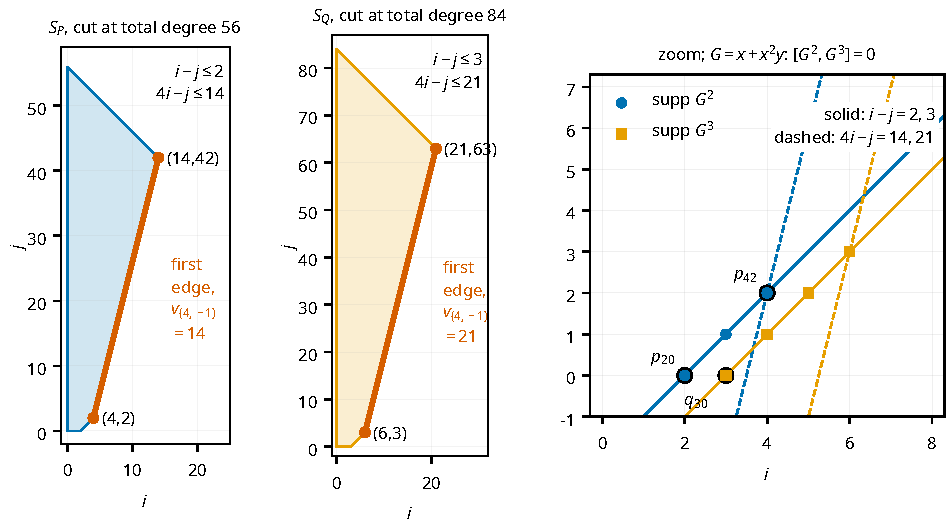
\includegraphics[width=\linewidth]{figures_jac/figJ6_cstar_support.pdf}
\caption{The chain $C^*$ at degree $(56,84)$ is excluded by half-plane support conditions, and the hypothesis $\mu\neq0$ cannot be dropped. Left and centre: the supports $S_P=\{i-j\le2,\ 4i-j\le14\}$ and $S_Q=\{i-j\le3,\ 4i-j\le21\}$, cut at total degree $56$ and $84$ for orientation. The thick edge is the first edge $(7,21)\to(2,1)$ scaled by $2$ and $3$: $(14,42)$--$(4,2)$ and $(21,63)$--$(6,3)$. Right: a zoom on the corner, with the coefficients $p_{20}$, $p_{42}$, $q_{30}$ (circled) that the theorem requires to be nonzero, and the supports of $G^2$ and $G^3$ for $G=x+x^2y$. These supports lie on the boundary lines and satisfy every hypothesis except $\mu\neq0$, while $[G^2,G^3]=0$. The statements \texttt{cstar\_no\_pair\_firstEdge} and \texttt{cstar\_no\_pair\_deg} are Lean kernel theorems. The row stays at grade B, because the passage from the printed row to \texttt{FirstEdgeCstar} is a reading and because the row matters only if the enumeration premise and the reduction chain hold.}
\label{rp:fig:cstar}
\end{figure}

\subsection{The certificate}

The coefficient comparison produces a finite system of polynomial equations in the unknown coefficients. The second form of the exclusion is a certificate for that system: $1$ lies in the ideal generated by $55$ polynomials in $70$ variables over $\mathbb Q$ (\texttt{W9.\allowbreak{}CstarBridge.\allowbreak{}one\_\allowbreak{}mem\_\allowbreak{}span}). A certificate of this kind excludes solutions over every field of characteristic zero for an elementary reason. If $1=\sum_k c_kg_k$ with $c_k\in\mathbb Q[z_1,\dots,z_{70}]$, and if a point $z\in K^{70}$ satisfied $g_k(z)=0$ for all $k$, then evaluating at $z$ would give $1=0$. The theorem \texttt{no\_\allowbreak{}common\_\allowbreak{}zero\_\allowbreak{}field} is this conclusion, proved in the kernel for an arbitrary field $K$ of characteristic zero. The certificate is graded 4K as a statement, and the elimination, as a chain, B.

Two encodings of the same system were written, one from the support form and one from the generator list, and a third theorem joins them: \texttt{W10.\allowbreak{}CstarLink.\allowbreak{}span\_\allowbreak{}eq} proves that the two ideals are equal, \texttt{one\_\allowbreak{}mem\_\allowbreak{}span\_\allowbreak{}w6b} transfers the certificate, and \texttt{cstar\_\allowbreak{}no\_\allowbreak{}pair\_\allowbreak{}gen2} restates the support-form exclusion through the second encoding. The bridge between the encodings is graded kernel-verified, I1; it is a bridge between two Lean encodings and not a comparison with the printed GGHV text.

\subsection{The first-edge form}

The support hypotheses of \texttt{cstar\_\allowbreak{}no\_\allowbreak{}pair} are strong, and a reader may ask whether they follow from the data that define the row. They do. The structure \texttt{FirstEdgeCstar} asks only that every monomial $x^iy^j$ of $P$ satisfy $4i\le j+14$, that is, $v_{(4,-1)}(P)\le14$, and that $p_{42}\ne0$. The kernel theorem reads as follows.

\begin{leanlisting}{\texttt{W15-CERT/lean/W15Cert/CstarF.lean}, lines 76--78 and 83--86, verbatim; the two-line proof of the first theorem (file lines 79--80) is omitted and described below.}{rp:lst:cstar}
theorem cstar_no_pair_firstEdge [CharZero K] (P Q : MvPolynomial (Fin 2) K) (μ : K) (hμ : μ ≠ 0)
    (hJ : W6B.jac P Q = C μ) (hr : 3 * P.totalDegree = 2 * Q.totalDegree)
    (hP1 : 1 < P.totalDegree) (hE : FirstEdgeCstar P) : False := by
  ...

theorem cstar_no_pair_deg [CharZero K] (P Q : MvPolynomial (Fin 2) K) (μ : K) (hμ : μ ≠ 0)
    (hJ : W6B.jac P Q = C μ) (hdP : P.totalDegree = 56) (hdQ : Q.totalDegree = 84)
    (hE : FirstEdgeCstar P) : False :=
  cstar_no_pair_firstEdge P Q μ hμ hJ (by omega) (by omega) hE
\end{leanlisting}

The proof has two steps. The lemma \texttt{cstar\_\allowbreak{}chain} derives the half-plane supports and the nonvanishing of $p_{20}$ and $q_{30}$ from the Keller condition, the ratio $3\deg P=2\deg Q$ and the first-edge datum; then \texttt{W6B.\allowbreak{}cstar\_\allowbreak{}no\_\allowbreak{}pair} applies. The second theorem is the specialization to the literal degrees $(56,84)$, where $\deg P=56$ and $\deg Q=84$ give $3\cdot56=168=2\cdot84$. These implications are graded 4K/I1. The row itself stays at grade B, because the passage from the printed row to \texttt{FirstEdgeCstar} is a reading of the row definition, and because the row only matters if the enumeration premise and the reduction chain hold.

A further tool developed in this period is a gauge lemma (Lemma~G). In a row's normal form, part of the freedom in $(P,Q)$ is a change of variables that does not alter the prescribed top forms; the lemma says that if at each depth the pivot map $H\mapsto(\text{coefficients of }[H,R^m])$ is onto the gauge coordinates, then every solution can be moved to one whose gauge coordinates vanish, so emptiness of the gauge-fixed system implies emptiness of the original (\texttt{W10Gauge.\allowbreak{}gauge\_\allowbreak{}elim}). The ingredient went from C to 4K; its faithfulness to the hand argument is B/I1.

\section{A gap in the Puiseux-free proof of the degree-84 row}\label{rp:sec:lambda}

GGHV give a second proof of the exclusion of the row with $\mathcal A_0=(7,21)$, the row of degree $(56,84)$ just discussed, in their \S5, and that proof avoids Puiseux series. It writes $C=P^{1/2}$ in $K[y,y^{-1}]((x^{-1}))$ and seeks $\tilde Q=\tilde C^3+\lambda\tilde C^{-1}+\tilde F$, where $\lambda$ is the coefficient of $C^{-1}$. A finite system of twelve equations in the coefficients $d_k(y)$ of the shifted series follows, and the argument ends by observing that a certain right-hand side is not the square of a polynomial because $\alpha$ and $\lambda$ are nonzero. A reading of \S5 on November 23, 2026 found that nothing there proves $\lambda\ne0$. Since $[C^2,C^{-1}]=0$, the Jacobian condition does not see $\lambda$ at the order where the system is set up, so there is no evident reason for it to be nonzero.

At $\lambda=0$ the system has solutions, and they are explicit. The final relation becomes
\[
(27\alpha^9d_0-2y^9)^2=108\,\alpha^{13}y^8 .
\]
Put $27\alpha^9d_0=2y^9+\beta y^4$. Then the left side is $(\beta y^4)^2=\beta^2y^8$, so the relation holds exactly when $\beta^2=108\,\alpha^{13}$. With $\alpha=3$ we have $108\cdot3^{13}=4\cdot27\cdot3^{13}=4\cdot3^{16}=(2\cdot3^8)^2$, so $\beta=\pm2\cdot3^8$ works. More generally $\alpha=3t^2$, $\beta=2\cdot3^8t^{13}$ gives $\beta^2=4\cdot3^{16}t^{26}=108\cdot3^{13}t^{26}=108\,\alpha^{13}$ for every $t\ne0$. Completing the remaining coefficients, all twelve equations vanish identically, every $d_k$ is a polynomial with $\deg d_k\le9-3k$, and the solution lies within GGHV's degree bounds. Singular, SymPy and FLINT (the last on the full system of $402$ coefficient generators) agree, so the witness is grade B. With $\lambda$ left free, the same point leaves exactly one equation unsatisfied, $Q_3=\lambda y^8$, which shows that $\lambda\ne0$ is precisely the input the printed argument uses. This is a gap in the printed argument, not a counterexample: the \S5 system is only a consequence of the Jacobian condition, and its solutions need not come from Keller pairs.

Later the same day we closed the gap by excluding the branch $\lambda=0$ directly. After the shift $X\mapsto X-c(y)$ with $\deg c\le3$, the full Jacobian condition in the $\lambda=0$ family becomes the equation
\[
\text{(E)}\qquad y\,[P',Q']-6P'_X\,Q'+4P'\,Q'_X=(X-c)\,y^9 ,
\]
which is linear in the unknown coefficients of $Q'$ and of $c$. The resulting linear system is inconsistent: FLINT at several values of $t$, Singular with $t$ symbolic (where $1$ lies in the ideal), and an independent generator written in Singular alone all agree, and a positive control of the right shape is consistent of dimension $8$. The exclusion of the $\lambda=0$ branch is graded B, raised to I2 by an independent re-derivation in a separate environment, which also rejected all five planted controls given to it. Still on November 23 the reduction from the Jacobian condition to (E) was chained in the kernel: \texttt{W9R.\allowbreak{}lam0\_\allowbreak{}hat}, \texttt{W9R.\allowbreak{}lam0\_\allowbreak{}cleared} and \texttt{W9R.\allowbreak{}lam0\_\allowbreak{}no\_\allowbreak{}partner} go from $[P,Q]=x$, through the shift and the bound on the weighted degree of $\hat Q$, to the inconsistency of (E). The overall exclusion stays B, conditional on GGHV's own premises at this point (completeness of the family, the Newton polygon of $Q$, and $\deg c\le3$). Neither~\cite{GGV1} Theorem~2.6 nor the companion papers supply $\lambda\ne0$ either, so the printed sentence remains unproved as written; it is simply no longer needed.

\section{Lemma B and Lemma S}\label{rp:sec:lemmaB}

Lemmas B and S concern the bottom row of a Laurent Keller pair and feed the analysis of the slot in \S\ref{rp:sec:slot}. We work with finitely supported functions $f,g:\mathbb Z^2\to K$, regarded as Laurent polynomials $\sum f(i,j)x^iy^j$, with the bracket extended in the obvious way. Suppose $[f,g]=c\,x^{-2}$ with $c\ne0$, both supports have nonnegative $y$-exponents, the smallest $x$-exponent in the support of $f$ is $-m$, and the row of $f$ at $x$-exponent $-m$, read as a polynomial in one variable, equals $\lambda\sigma^m$. Lemma B says something about the polynomial $\sigma$, and Lemma S turns that into a statement of shape.

\begin{definition}\label{rp:def:rf}
A nonzero polynomial $\sigma\in K[X]$ is \emph{residue-free} if there are $H\in K[X]$, an integer $t\ge0$ and a constant $c\ne0$ with
\[
H'\sigma-tH\sigma'=c\,\sigma^t .
\]
\end{definition}

The name is explained by the quotient rule. For any $H$ and $t$,
\[
\Bigl(\frac{H}{\sigma^t}\Bigr)'=\frac{H'\sigma^t-H\cdot t\sigma^{t-1}\sigma'}{\sigma^{2t}}=\frac{H'\sigma-tH\sigma'}{\sigma^{t+1}} .
\]
So the defining identity holds if and only if $(H/\sigma^t)'=c/\sigma$: the rational function $c/\sigma$ is a derivative. A derivative of a rational function has residue zero at every pole, since the derivative of a Laurent series has no term in $(X-r)^{-1}$. Hence a residue-free $\sigma$ has $1/\sigma$ with all residues zero.

This is strictly stronger than having no simple root, and the example that separates the two conditions is the one behind a correction to our own earlier results. Take $\sigma=X^2(X-1)^2$. It has no simple root. Its partial fraction decomposition is
\[
\frac{1}{X^2(X-1)^2}=\frac{2}{X}+\frac{1}{X^2}-\frac{2}{X-1}+\frac{1}{(X-1)^2},
\]
so the residues at $0$ and $1$ are $2$ and $-2$, and $\sigma$ is not residue-free. The kernel theorems \texttt{W15S.\allowbreak{}not\_\allowbreak{}RF\_\allowbreak{}two\_\allowbreak{}roots} and \texttt{nsr\_\allowbreak{}two\_\allowbreak{}roots} prove both facts.

On November 23 and 24, 2026 we reported Lemma~B ``for every $m$'' as a kernel theorem (\texttt{W12S.\allowbreak{}lemmaB\_\allowbreak{}prime}, \texttt{W13B.\allowbreak{}lemmaB\_\allowbreak{}all}, \texttt{lemmaB\_\allowbreak{}every}). Reading the statements as text on November 24 showed that all of them conclude only that $\sigma$ has no simple root (errata E171). Those theorems are correct as stated, but they cannot feed Lemma~S, which needs the residue-free form; what was overstated was the reading of them as the Lemma~B that Lemma~S consumes. The repair is \texttt{W15R.\allowbreak{}lemmaB\_\allowbreak{}every\_\allowbreak{}rf}, with the same hypotheses, for every $m\ge1$, concluding that $\sigma$ is residue-free. It is graded 4K/I1.

\begin{leanlisting}{\texttt{W15-LEAN/lean/W15\_LemmaS.lean}, lines 28--29 and 268--269; statement verbatim, proof elided, except that the type $\mathbb N$ is written \texttt{Nat}, which Lean reads as the same type.}{rp:lst:lemmaS}
def RF (σ : K[X]) : Prop :=
  ∃ (H : K[X]) (t : Nat) (c : K), c ≠ 0 ∧ derivative H * σ - C (t : K) * H * derivative σ = C c * σ ^ t

theorem lemmaS {K : Type*} [Field K] [CharZero K] [IsAlgClosed K] {σ : K[X]} (hσ : σ ≠ 0)
    (hrf : RF σ) : ∃ r : K, σ = C σ.leadingCoeff * (X - C r) ^ σ.natDegree :=
\end{leanlisting}

Lemma~S says that over an algebraically closed field a residue-free polynomial is a constant times a power of one linear factor. Its proof in the kernel is algebraic, by counting degrees, with no appeal to the Riemann--Hurwitz formula; hand grade B/I1 became 4K/I1. Combining the two, \texttt{W15R.\allowbreak{}bottom\_\allowbreak{}prime\_\allowbreak{}power} shows that under the Keller condition and the bottom-row hypothesis (we call it hF) $\sigma=\mathrm{lc}(\sigma)\,(X-r)^{\deg\sigma}$ with $\deg\sigma\ne1$, again 4K/I1.

The hypothesis hF deserves comment. When $\gcd(m,b)=1$, where $b$ is the bottom exponent of $g$, it is discharged by the earlier \filename{W5F.lemmaU\_bottom} (\filename{W15W.lemmaB\_coprime}, 4K/I1). When $\gcd(m,b)>1$ it is not a consequence of the Keller condition: \filename{W15W.hF\_not\_from\_keller} refutes that implication in the kernel by an explicit pair, so hF stays a premise for those rows. Later on November 24 we generalized Lemma~U to bottom rows of the form $\lambda H^{m/d}$, $\mu H^{b/d}$ (\filename{W16U.lemmaU\_bottom\_gen}) and proved Lemma~D, a descent along the bottom chain, for every exponent $e\ge1$ (\filename{W16D.lemmaD\_chain}, 4K/I1). The statement of Lemma~D needs $c\ne0$; for $c=0$ there is the explicit counterexample $f=x^{-1}w$, $g=x^{-2}w^2$.

\section{Orevkov's construction and its misprints}\label{rp:sec:orevkov}

Orevkov's paper~\cite{Orevkov2001} constructs a map with one dicritical at infinity that satisfies every combinatorial condition at infinity a Keller map would, and is still not an embedding; it is the standard warning that information local at infinity cannot decide the conjecture. We transcribed the linear system of his \S4.2 into Lean, where it depends on two parameters $(A_2,A_3)$. One polynomial certificate, valid in every commutative ring and for every value of the parameters, shows that the conditions imposed by the hulls force the linear form that Orevkov uses to derive his contradiction to vanish (\texttt{W13O5.\allowbreak{}P\_\allowbreak{}all.\allowbreak{}orev42\_\allowbreak{}all}). This certificate should not be confused with obligation O5 of Part~III, which concerned the chart step of Lemma~\ref{td:lem:e1} and the binary-form step of Lemma~\ref{td:lem:linf}. That obligation was met on November 22, 2026: the binary-form lemma is grade A with the added hypothesis $g\ne0$ (a kernel-checked counterexample shows the printed lemma false without it), and the polynomial identities of the chart step are grade A, while the rational-function reading stays B.

The Orevkov certificate is graded 4K/I1 for the system as transcribed, and a separate audit compared the transcription with the printed text (English edition, pp.~23--24, and the Russian original, p.~202): it is graded faithful, B/I1, as a reading. Re-deriving the polygons from the blow-up data alone also clarified two misprints. Lemma~4.1(c) prints the factor $(1+y_{10'})^{-6a}$ in both editions, while Figure~22 (height $27=9a$ at $a=3$), the vertex $(-6a,-9a)$, Lemma~4.2 and Figure~23 all fit an exponent of magnitude $9a$. The re-derivation gives the pole order $p_7=9a$ along the seventh exceptional curve, $27$ at $a=3$ and $180$ at $a=20$, which supports the reading that $-6a$ is a misprint for $-9a$. The misprint diagnosis was first graded C (errata E23); the re-derivation from the blow-up data is graded B/I1 (errata E173, which amends E23), and the misprint has not been confirmed by the author. The same re-derivation found that a vertex of the polygon $P_{10'}$ labelled $(0,-1)$ is in fact $(-1,0)$ (B/I1, also unconfirmed). Orevkov's conclusion, the contradiction of \S4.2 from $Q$ alone at $a=3$, is reproduced and unaffected.

\section{The chain through van den Essen's Chapter 10}\label{rp:sec:vde}

Layer (i) of the enumeration premise is the normal-form theorem of~\cite{GGV1}, and its proof runs through results of Chapter~10 of van den Essen's book~\cite{vdE2000}. Reading the book's chain in full showed that it uses no Puiseux series. We have since formalized the chain result by result.

The first point of interest is Lemma~10.2.4 (p.~246), which concerns two $w$-homogeneous polynomials $f,g$ with $[f,g]=0$. Its part (i), as printed, asserts that both are constant multiples of powers of a single $w$-homogeneous $h$. This is false when the $w$-degree of $h$ is zero. Take $w=(1,-1)$, $f=xy$, $g=x^2y^2+xy$. Both have $w$-degree $0$, and $[f,g]=0$ because $g=f(f+1)$ is a polynomial in $f$. Since $f=x\cdot y$ is a product of two distinct primes, $f=c\,h^n$ forces $h\sim xy$ and $n=1$; but $g$ has two terms, so it is not a constant times a power of $xy$ (errata E90, grade B). The fix is to add the hypothesis that $f$ or $g$ has nonzero $w$-degree; we read every use in Chapter~10 and in~\cite{GGV1} as satisfying it (a reading, grade C; derived in the kernel for 10.2.5), so the defect appears harmless. The corrected statement is the kernel theorem \texttt{W14Z.\allowbreak{}vdE\_\allowbreak{}10\_\allowbreak{}2\_\allowbreak{}4} (4K/I1), and the printed form is refuted in the kernel by \texttt{printed\_\allowbreak{}10\_\allowbreak{}2\_\allowbreak{}4\_\allowbreak{}i\_\allowbreak{}false}, using exactly the example above; the faithfulness of that refutation to p.~246 is a reading, grade B.

The rest of the chain is now in the kernel. Theorems 10.2.3, 10.2.5, 10.2.6, 10.2.7 and the core of 10.2.10 were formalized on November 24, 2026, and later the same day the normal form 10.2.12 and then 10.2.8 in full (\texttt{vdE\_\allowbreak{}10\_\allowbreak{}2\_\allowbreak{}8}, 4K/I1, faithfulness B/I1). On November 25 we added 10.2.13 (which the book leaves as an exercise), 10.2.15, the cases of 10.2.17, the numerical part of 10.2.19 and case (i) of 10.2.18. Later that day we completed 10.2.18 in its three cases and proved 10.2.21 by strong induction on the degree drop, over an algebraically closed field of characteristic zero: for a Keller pair there is an automorphism $\alpha$ with $\deg\alpha P\le1$ or $\deg\alpha Q\le1$, or $\alpha P$ lies in the box of the normal form (\texttt{W19Z.\allowbreak{}vdE\_\allowbreak{}10\_\allowbreak{}2\_\allowbreak{}18}, \texttt{W19Z.\allowbreak{}vdE\_\allowbreak{}10\_\allowbreak{}2\_\allowbreak{}21}, both 4K/I1). Two gaps between the book and~\cite{GGV1} were then closed: a pair with a linear component is an automorphism, and the descent from an algebraic closure back to the base field holds, in the form ``JC(2) over an extension $E$ implies JC(2) over $L$'' (\texttt{W19Z2.\allowbreak{}isAut\_\allowbreak{}descent}, \texttt{W19Z2.\allowbreak{}jc\_\allowbreak{}descent}). The ``Theorem central'' of~\cite{GGV1} was proved as \texttt{W19Z5.\allowbreak{}centralOpen} (4K/I1).

The literature notes from this reading are minor and we record them briefly. In the proof of 10.2.18, case (ii) is left to the reader as an exercise and case (iii) is reduced to an earlier case by exchanging $X$ and $Y$; this is an omission, not a false step (E219). On p.~252 the exponent $v_0$ is given as $b-\sum n_i$ where the definition gives $b-u\sum n_i$; the two agree because the proof has already shown $u=1$ (E220). The notations $T(k,2)$ and $T(2,k)$ are interchanged between statement and proof (E221). On p.~253, line~2 compares $\deg_Y\varphi(Y)$ with $\deg_YP$ where the argument needs $\deg_Y\varphi(P)$ (E222). Separately, the book uses on p.~249 the commutation $[P,P^{j/n}]=0$ without proving it; this is a gap in exposition, not an error. Case (ii) of 10.2.18 also needs the field to be algebraically closed: over $\mathbb R$ the form $(X^2+Y^2)^n$ has no linear factor (E91).

With these pieces, the normal-form theorem of~\cite{GGV1} (the proposition titled ``primera condici\'on est\'andar'') is a kernel theorem without the Cassou-Nogu\`es premise. The kernel first proves the needed Cassou-Nogu\`es statement \texttt{W19Z7.\allowbreak{}cn2011} and then \texttt{W19Z7.\allowbreak{}primera\_\allowbreak{}ekua4}: over an algebraically closed field, a Keller pair that is not an automorphism and has minimal $\gcd(\deg P,\deg Q)$ among such pairs can be moved by an automorphism into the box with the standard conditions. The printed form is \texttt{W19Z8.\allowbreak{}primera\_\allowbreak{}printed}, and \texttt{W19Z8.\allowbreak{}jc2\_\allowbreak{}of\_\allowbreak{}noNF} states the consequence: JC(2) over $L$ follows if no pair over $\bar L$ is in that normal form. All are 4K/I1. Layer~(i) of the enumeration premise is thereby a standalone kernel theorem, but the link from it to the rows is a reading, and the enumeration premise as a whole stays B.

\section{Rows 175, 168 and 120}\label{rp:sec:rowsdetail}

\subsection{Row 175}

Row~175 has first edge from $(10,25)$ to $(2,1)$, $(m,n)=(2,5)$, and degrees $(70,175)$; GGHV never printed it, because it is CN-only. Its exclusion is a certificate of the same kind as for $C^*$: $1$ lies in the ideal of $105$ generators in $135$ variables over $\mathbb Q$, a kernel certificate completed on November 23, 2026 (algebra 4K/I1). The kernel proof was replayed independently with Lean's \texttt{leanchecker}: all $1225$ modules passed, with no failures. On November 24 we derived the support premise P-b from the first-edge datum (\texttt{W14.\allowbreak{}R175F.\allowbreak{}chain\_\allowbreak{}of\_\allowbreak{}firstEdge175}) and stated the elimination with the ratio $5\deg P=2\deg Q$ rather than the literal degrees (\texttt{r175\_\allowbreak{}no\_\allowbreak{}pair\_\allowbreak{}firstEdge}). The row is graded B, and the grade will not be raised while the enumeration premise is B.

\subsection{Row 168}

Row~168 has $(m,n)=(2,3)$ and degree $(112,168)$. After a hand reduction (which we label C1) to two gauge-fixed normal forms, indexed by a coefficient $s_0\in\{0,1\}$, the case $s_0=1$ was eliminated by an exact certificate on November 23, 2026 (B/I1) and later in the kernel (\texttt{W12.\allowbreak{}R168s1L.\allowbreak{}row168F\_\allowbreak{}no\_\allowbreak{}solution}). The case $s_0=0$ depends on a parameter $r_1$, and the branches $r_1=2$ and $r_1=-2$ are related by a symmetry, which we now verify.

Let $P,Q\in\mathbb Q(i)[x,y]$ and put $\tilde P(x,y)=P(ix,iy)$, $\tilde Q(x,y)=-Q(ix,iy)$. By the chain rule $\tilde P_x=i\,P_x(ix,iy)$, $\tilde P_y=i\,P_y(ix,iy)$, $\tilde Q_x=-i\,Q_x(ix,iy)$ and $\tilde Q_y=-i\,Q_y(ix,iy)$. Therefore
\[
[\tilde P,\tilde Q]=(i)(-i)\bigl(P_xQ_y-P_yQ_x\bigr)(ix,iy)=-i^2\,[P,Q](ix,iy)=[P,Q](ix,iy).
\]
If $[P,Q]=\mu$ is constant, then $[\tilde P,\tilde Q]=\mu$ as well, so the substitution carries Keller pairs to Keller pairs with the same constant. The sign in front of $Q$ is what makes the factor $i\cdot(-i)$ equal to $1$; without it the constant would change to $i^2\mu=-\mu$, and the planted check of that sign was rejected as expected. (By contrast, $y\mapsto-y$ alone multiplies the bracket by $-1$.) This substitution maps the normal form of the branch $r_1=-2$ onto that of $r_1=2$, as $228$ generators matched in two tools show, and the kernel theorem \texttt{W13.\allowbreak{}S0.\allowbreak{}minus2\_\allowbreak{}of\_\allowbreak{}plus2} transfers the inconsistency of the $r_1=2$ system to the $r_1=-2$ system over every field of characteristic zero, through $229$ symmetry identities. The branch $r_1=2$ itself was closed by a complete tree of $65$ nodes with no open node.

Of the remaining branch hypotheses, the one called h010 is a kernel theorem (\filename{W16.GlueHa.h010}, 4K/I1), and the joined statement \filename{W16.R168J.row168\_joint16a} is a kernel theorem conditional only on the generic-$r_1$ hypothesis hgen, together with the hand reduction C1 and the enumeration premise. Row~168 is graded B/I1. The build that would discharge hgen in the kernel was still running at the close of work on November 25, 2026, so the unconditional joined theorem does not exist yet.

\subsection{Row 120}

Row~120 has $(m,n,g)=(3,2,4)$ and degree $(120,80)$. Its analysis splits on a coefficient $f_5$. The branch $f_5\ne0$ is closed, B/I1. The branch $f_5=0$ is open. Its tree has been partly decided: the nodes 0011010, 001101110 and 001101100 are inconsistent (B/I1), the leaves 001101100 and 001101111100 are closed at B/I1 (both resting on the premise that the layer core lies in the node ideal), and the leaf 001101101000 is C/I1. The obstacle is that the core of node 001101 at layer~13 is a non-empty rational open threefold (C/I1), so the system becomes inconsistent, if at all, only at a deeper layer. A gauge instance for this row is in the kernel (\texttt{W10Gauge.\allowbreak{}Row120.\allowbreak{}row120\_\allowbreak{}gauge\_\allowbreak{}elim}, 4K/I1), but it is a reduction, not an elimination.

\section{The CN-only rows and the cover}\label{rp:sec:w19}

The CN-only rows need the Cassou-Nogu\`es condition, which until then had been a premise. On November 25, 2026 it was proved in the form used by the rows. Define $\mathrm{CNAt}(P,Q)$ to mean: if $[P,Q]$ is a nonzero constant, then the face of the support of $P$ on which $i-j$ is largest consists of a single point. The kernel theorem \texttt{W19.\allowbreak{}Wire.\allowbreak{}cnat} proves $\mathrm{CNAt}(P,Q)$ for all $P,Q$ over every field of characteristic zero, by a local residue computation at one root in a simple algebraic extension. The face condition is not empty: for $P=y+x^2$ the maximum of $i-j$ over the support $\{(0,1),(2,0)\}$ is $2$, attained only at $(2,0)$, consistent with the theorem. A second premise, a support-level form of~\cite{GGV1} Theorem~2.6 at a direction $w$ (the predicate $\mathrm{T26At}$), is now the kernel theorem \texttt{W19.\allowbreak{}T26.\allowbreak{}t26at}, and the counting lemma of~\cite{GGV1} called ``Lema Joseph'' is \texttt{joseph\_\allowbreak{}lemma}. All three are 4K/I1.

Applying these theorems to the rows uncovered an error in our own earlier results, which we report in full because it changes what the earlier row theorems can be said to have shown. For each row, the \emph{terminal} theorem is the last theorem of its chain, the one that derives a contradiction from the row's data. For $99$ of the $166$ unblocked rows the terminal theorem carried an added hypothesis, \texttt{hEd}, asserting a second support point on the top line of slope $-1$ through the final corner. For $97$ of those rows \texttt{hEd} contradicts the row's own half-planes (59 kernel theorems \texttt{W19.\allowbreak{}VoidHEd.\allowbreak{}void\_\allowbreak{}row\dots}, confirmed by Python and Singular scans). A theorem with contradictory hypotheses is true and eliminates nothing, so those terminals were vacuous (errata E238). The cause was that the Cassou-Nogu\`es datum had been attached to the wrong stage of the chain: in all $99$ rows the condition that was dropped from the printed enumeration applies at stage $0$, to the pair before any transformation of the chain. The rows were rewired to the stage-$0$ datum (66 theorems \texttt{W19.\allowbreak{}Stage0.\allowbreak{}s0\_\allowbreak{}\dots}), with the data checked satisfiable apart from the Keller condition in SymPy and Singular, and every rewired theorem was then checked non-vacuous in two tools. A further $27$ rows whose relaxation sits on a transformed stage-1 pair were re-justified after the kernel showed that the stage map is $y\mapsto y+c$, so the stage-1 pair is again a polynomial Keller pair (E239a). The final count is that all $193$ unblocked and blocked CN-only rows ($166+27$) are eliminated in the kernel: $87$ from the Keller condition and the original chain data, and $106$ from the Keller condition and their defining slope-1 datum at the correct stage. The rows stay at grade B, because of the R-def reading and the enumeration premise.

Layer~(ii) of the enumeration premise was then reduced to a single Lean proposition. A row is modelled as a ratio $(m,n)$ and a predicate $D$ on $P$, its first-edge datum. A row is \emph{killed} if no Keller pair with $n\deg P=m\deg Q$ and $\deg P>1$ satisfies $D$, and a list of rows \emph{covers} if every pair in the normal form of \S\ref{rp:sec:vde}, after a coordinate change, carries the datum of some listed row. We then proved that a covering list of killed rows gives JC(2) over every field of characteristic zero (\texttt{W19Z9.\allowbreak{}jc2\_\allowbreak{}of\_\allowbreak{}cover}), refined the covering condition to the column-positive, aligned form \texttt{CoversAutAl}, and supplied $124$ terminal theorems for CN-only rows in the form of killed rows.

\begin{leanlisting}{\texttt{W19-ZAR10/lean/W19Z10\_Ref.lean}, lines 11--15; statement verbatim, proof elided.}{rp:lst:cover}
theorem jc2_of_coverCN {L : Type} [Field L] [CharZero L]
    (rest : List (W19Z9.RowT (AlgebraicClosure L))) (hk : ∀ r ∈ rest, W19Z9.Kills r)
    (hc : CoversAutAl (Kill.rowsCN ++ rest)) :
    ∀ (P Q : MvPolynomial (Fin 2) L) (c : L), c ≠ 0 → W13Z.br P Q = C c →
      W19Z.IsAut (W19Z2.pairHom P Q) := by
\end{leanlisting}

The theorem is 4K/I1 as an interface. Its content is a reformulation, and we stress what it does not say. The two hypotheses \texttt{hk} and \texttt{hc} are exactly what remains of the enumeration premise: a list \texttt{rest} of further rows, each killed, such that together with the CN-only rows they cover every normal-form pair. Supplying \texttt{hc} is the completeness of the GGHV and~\cite{GGV1} enumeration, and this needs regular-corner conditions and a degree bound that are not yet in Lean. Layer~(ii) stays B.

A different reduction concerns a sub-problem on the bottom chain that we label SP-W4, which arises in the slot of \S\ref{rp:sec:slot} for bottom exponent $a_0\le-2$. It carries a parameter $\gamma$ in its top condition. At $\gamma=0$ the full list of hypotheses is contradictory (\texttt{W19W.\allowbreak{}spw4\_\allowbreak{}gamma0\_\allowbreak{}false}, 4K/I1), and an earlier case R is excluded as well. For $\gamma\ne0$ the problem is open and, by the following argument, of the strength of JC(2) itself: in the chart $v=z/x^2$ a survivor becomes a polynomial Keller map of the $(x,v)$-plane that stays bounded along a branch $x\to\infty$, $v\sim\gamma x^{-2}$, hence is not proper and would be a counterexample.

\section{The last step: proper Keller maps}\label{rp:sec:F3}

Part~III's argument from Theorem~R to JC(2) uses the fact (F3): a Keller map $F$ is an automorphism if and only if its non-properness set $S_F$ is empty. Part~III gave the classical argument: if $S_F=\emptyset$, then $F$ is a finite étale cover of the simply connected plane, hence an isomorphism. This step is classical. In this period it was formalized, and we report it as a formalization, not as new mathematics.

Over $\mathbb C$, \texttt{W19TOP4.\allowbreak{}proper\_\allowbreak{}keller\_\allowbreak{}automorphism\_\allowbreak{}uncond} proves that a polynomial map of $\mathbb C^2$ with Jacobian determinant a nonzero constant, under which preimages of compact sets are compact, has a two-sided polynomial inverse. The route is analytic: bijectivity and the inverse function theorem give a holomorphic inverse, a root bound gives uniform polynomial growth along lines, and Cauchy estimates and interpolation show the inverse is polynomial. We checked that the hypotheses are only the nonzero constant $c$, the Jacobian identity and properness, and that the map $(x^2,y)$, proper but not Keller, fails the conclusion, so the Keller hypothesis does real work. Over an arbitrary field $K$ of characteristic zero, the algebraic version is \texttt{W19TOP5.\allowbreak{}F3\_\allowbreak{}field\_\allowbreak{}iff}: if $[P,Q]=c\ne0$, then $(P,Q)$ is an automorphism if and only if $K[x,y]$ is a finite module over $K[P,Q]$. Its two directions are \texttt{F3a\_\allowbreak{}field} and \texttt{F3b\_\allowbreak{}field}. All are 4K/I1.

Two readings connect these theorems to (F3) as printed. First, ``$S_F=\emptyset$'' is identified with ``$K[x,y]$ is finite over $K[P,Q]$''; second, the Lean predicate of being an automorphism is identified with the printed notion. Both readings are grade B, and the pointwise equality of the algebraic and the topological $S_F$ is not formalized.

The logical position is then as follows. Let $F$ be a Keller map, fix a point $c\notin S_F$, and let $N_\infty(c)$ be the number of dicriticals at infinity of the pencil $\Lambda_c$. Proposition~\ref{td:prop:count}(c) of Part~III gives
$$N_\infty(c)\ \ge\ 1+\#\{\text{components of }S_F\}.$$
Suppose Theorem~R holds for $F$, so that $N_\infty(c)\le1$. Then $1+\#\{\text{components of }S_F\}\le1$, hence $S_F$ has no components, that is, $S_F=\emptyset$; this is the argument of Proposition~\ref{td:prop:onedic}. The fact (F3) turns $S_F=\emptyset$ into ``$F$ is an automorphism''. Theorem~R for every Keller map would therefore give JC(2), which is one half of Proposition~\ref{td:prop:equiv}. The present formalization secures the last implication, from $S_F=\emptyset$ to automorphism, in the kernel, up to the two readings just named; the count itself remains grade B from Part~III. It does nothing for the hypothesis: Theorem~R remains open, and so does JC(2).

\section{The slot}\label{rp:sec:slot}

\subsection{The problem}

Part~III showed that every dicritical at infinity of a non-affine Keller map has depth at least $2$ (Corollary~\ref{td:cor:depth2}). Call a dicritical at infinity an $E_S$ if it maps onto an affine curve, that is, onto a component of $S_F$. On November 22, 2026 we excluded an $E_S$ at the end of a free chain of depth $3$ with $A=1$ (in our normalisation $A$ is the log discrepancy of the end divisor; on this chain the chart Jacobian $\partial(x,y)/\partial(\xi,\tau)$ equals $-1$), by a residue obstruction, and deduced that every $E_S$ of a Keller map has depth at least $4$ (grade B, I1). The first open configuration is a free chain of depth $4$ over $[1{:}0{:}0]$, which we call the \emph{slot}. In the chart $x=1/\xi$, $y=c\xi^2+\xi^3\tau$ with $c\ne0$, solving for $\tau$ gives
\[
\tau=\frac{y-c\xi^2}{\xi^3}=x^3y-cx ,
\]
and the ring of polynomials regular on the chart is $\mathcal O=K[y,\,xy,\,x^2y,\,x^3y-cx]$ (the Jacobian of the chart is $\partial(x,y)/\partial(\xi,\tau)=(-\xi^{-2})(\xi^3)-0=-\xi$). The case $c=-1$ is the ring $\mathbb C[Y,XY,X^2Y,X^3Y+X]$ of Wright~\cite{Wright1997}, which Wright names, after his Theorem~3.3, the simplest unresolved case of his Conjecture~3.2: that there is no counterexample to the Jacobian conjecture with both components in this ring (p.~601). In Wright's parametrization this is the case $m=3$, $\alpha_1=0$; his Theorem~3.3 settles the case $\alpha_1\ne0$. Wright's conjecture is not known to be equivalent to JC(2), so excluding the slot would settle a named open problem but would not prove JC(2). A realized slot does give a Keller pair in $\mathcal O$; the converse needs one more case, which we call case Z, so ``slot excluded'' is formally weaker than this case of Wright's conjecture.

One computation explains why the slot resists the residue arguments that work at smaller depth. For $\tau=x^3y-cx$ we have $[y,\tau]=y_x\tau_y-y_y\tau_x=0-(3x^2y-c)=c-3x^2y$ and $[xy,x^2y]=y\cdot x^2-x\cdot2xy=-x^2y$, so
\[
[y,\tau]-3\,[xy,x^2y]=c .
\]
A nonzero constant is a sum of brackets of elements of $\mathcal O$. Hence no linear functional $L$ on $\mathcal O$ with $L([P,Q])=0$ for all $P,Q\in\mathcal O$ can have $L(1)\ne0$, and no obstruction that is linear in the Jacobian (a residue, a period, a twisted residue) can exclude the slot (grade B, November 22, 2026).

Figure~\ref{rp:fig:slot} follows the curves $\tau=\mathrm{const}$ through the four blow-ups: in each panel watch whether the curves still meet in the circled centre; they part only in the last panel, on $E_4$.

\begin{figure}[htbp]
\centering
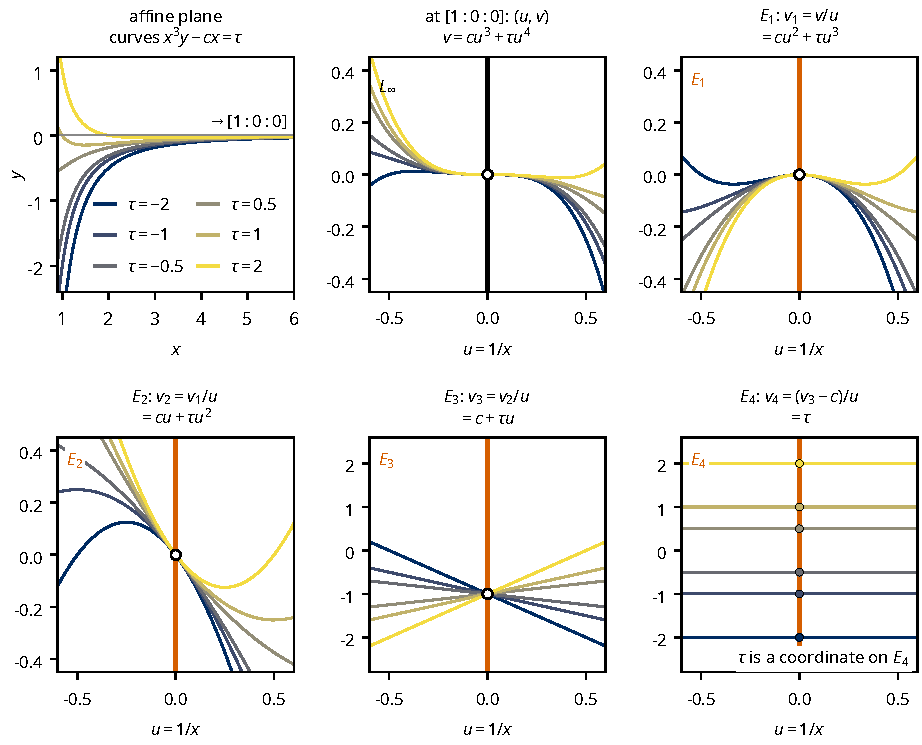
\includegraphics[width=\linewidth]{figures_jac/figJ5_slot_chain.pdf}
\caption{In the slot, the curves $x^3y-cx=\tau$ all pass through the first three centres and separate only on the fourth exceptional curve $E_4$, where $\tau$ is a coordinate. The chart is the one above, with $c=-1$, Wright's case. Top left: the real curves $\tau=\mathrm{const}$ for $x>0$, approaching $[1{:}0{:}0]$. The other panels use $u=1/x$, $v=y/x$ and then the successive blow-up charts $v_1=v/u$, $v_2=v_1/u$, $v_3=v_2/u$ and $v_4=(v_3-c)/u$; in them the curve is $v=cu^3+\tau u^4$, $v_1=cu^2+\tau u^3$, $v_2=cu+\tau u^2$, $v_3=c+\tau u$ and $v_4=\tau$. The vertical line is $L_\infty$ or $E_k=\{u=0\}$, and the open circle marks the next centre: $(0,0)$ three times, then $(0,c)$. Each centre is a free point of the newest exceptional curve. Every $E_S$ has depth at least $4$ (B/I1); the slot itself, condition R$\infty$, is open. The figure shows the geometry of the chart only, and says nothing about whether a Keller pair realizes it.}
\label{rp:fig:slot}
\end{figure}

\subsection{The formal computations}

We attacked the slot through a formal expansion. In the grading of $\mathcal O$ by $\deg X=-1$, $\deg Y=2$ that Wright suggests, one fixes the shape of a hypothetical pair (we work with the $(2,5)$ shape of genus~$1$) and solves $[P,Q]=c$ layer by layer in a band variable. At each order $m$ the new equations are linear in the new unknowns and are eliminated against pivots. A \emph{pivot stream} is the sequence, indexed by $m$, of the pivot coefficients at a fixed offset from the current order; six streams occur, at offsets $m-12$, $m-10$ and $m-5,\dots,m-2$. The \emph{run-A slice} fixes $t_1=1$ and a small set of other parameters. A \emph{window termination at $J$} would mean that the formal solution stops after layer $J$, so that $P,Q$ are polynomials of bounded degree; excluding it at $J$ excludes such pairs of the corresponding degree on the slice.

The results, with their grades, are these. All six pivot streams have exact closed forms (C/I1, empirical: fitted on $m\le25$ and matched exactly for $m=26,\dots,40$ on two slices, with a refit in Wolfram Engine over $m=26,\dots,45$). These forms were then derived for every $m\ge13$ on the run-A slice, by hand lemmas reducing order $m$ to a finite computation from order $m-13$ and an identity check in SymPy and Wolfram Engine (B/I1). For generic $t_1$ the four middle streams are rational functions of $(m,t_1)$, and they depend on $t_1$ through
\[
\kappa(t_1)=25-2t_1^2 ,
\]
which enters at the coefficient $p_{2,0}=(2t_1^2-25)/50=-\kappa/50$. With $q(m)=\kappa\,m(m+1)-1200$, one has, for instance, $L(m-2)=\frac{t_1}{3125}\cdot\frac{q(m)}{m}$. (The symbolic computations work in a shifted order variable $X$, fixed by how many layers they keep: $X=m-12$ in the run-A derivation, which keeps layers up to $13$, and $X=m-5$ in the generic-$t_1$ derivation, which keeps layers up to $6$; the forms printed here are in $m$.) These forms are B/I1, conditional on the hand lemmas of November 23 and on a generic-pattern hypothesis. The pivots vanish only on the countable exceptional set
\[
\Sigma=\{t_1\kappa(12t_1^2-25)=0\}\ \cup\ \{t_1:\ q(j)\,r(j)=0\ \text{for some integer } j\ge10\},
\]
where $r$ is an explicit cubic in $j$ with coefficients in $\kappa$. The second set starts at $j=10$ because the pivots at offset $m-3$ already involve $q(10)$ at $m=13$. That point is genuine: $q(10)=110\kappa-1200=0$ gives $\kappa=120/11$, and $120/11\ne1200/(j(j+1))$ for $j\ge13$. Earlier transient values belong to the same families; for example $q(7)/1000=(56\kappa-1200)/1000=\tfrac15-\tfrac{14}{125}t_1^2$, so the transient $t_1^2=25/14$ found on November 23 is the zero of $q(7)$. On November 25 we showed that the branches of $\Sigma$ are isolated for starting order $m_0\ge13$ (B/I1).

Figure~\ref{rp:fig:kappa} plots the four forms against the solver values; look at the bottom-left panel, where all seven values of $t_1$ fall on straight lines whose slopes are $\kappa(t_1)$, and at the residual panel, which is identically zero.

\begin{figure}[htbp]
\centering
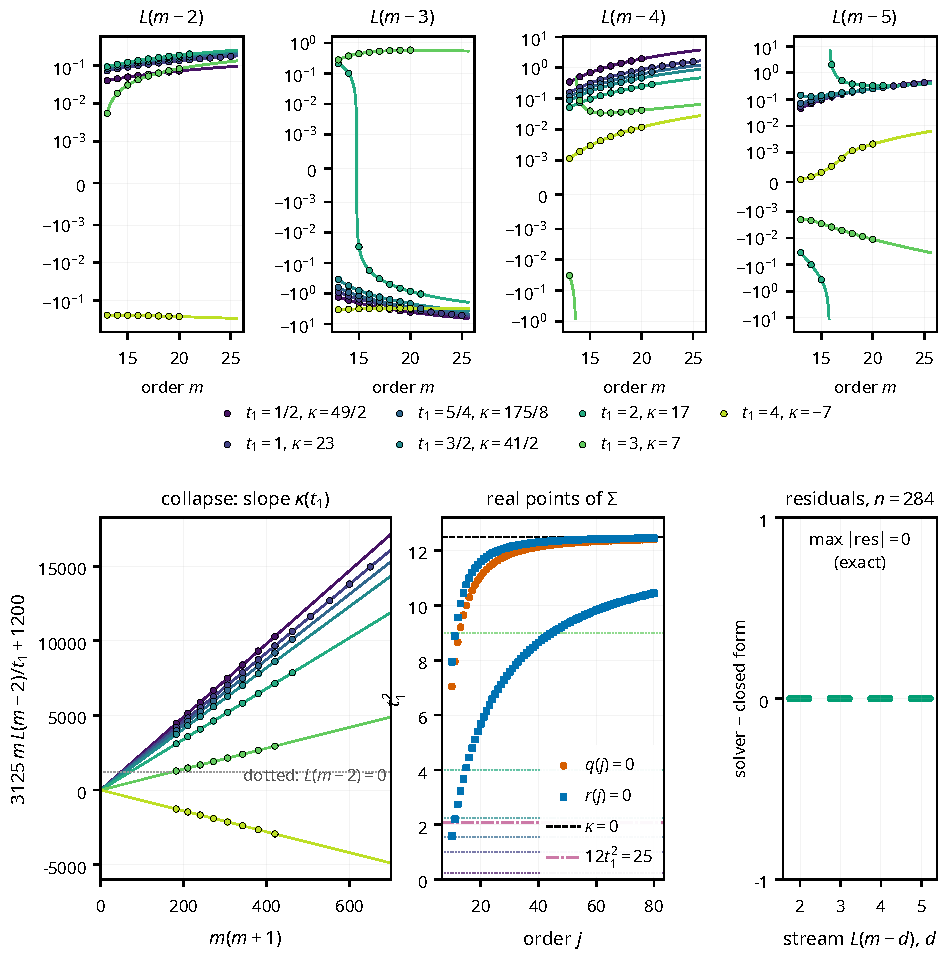
\includegraphics[width=\linewidth]{figures_jac/figJ3_kappa_law.pdf}
\caption{For generic $t_1$, the four middle pivot streams of the slot depend on $t_1$ only through $\kappa(t_1)=25-2t_1^2$, and they agree with the exact solver values. Top: the closed forms $L(m-2)=\tfrac{t_1}{3125}\tfrac{q(m)}{m}$, $L(m-3)=-\tfrac{r(m)}{1250\,m(m-1)}$, $L(m-4)=\tfrac{\kappa^3(m-6)\cdots(m-9)}{2500\,t_1(m-2)\,q(m-1)}$ and $L(m-5)=\tfrac{\kappa^4(m-6)\cdots(m-10)}{12500\,(m-3)\,r(m-1)}$, with $q(m)=\kappa m(m+1)-1200$ and $r(m)=\kappa^2m^3-350\kappa m^2+(1225\kappa-\kappa^2)m+7875(25-\kappa)$. The lines extend the forms to real $m$ as a guide; only integer $m$ is meaningful. The markers are the $284$ coefficients with $m\ge13$ at offsets $2,\dots,5$ from eight independent solver runs at $t_1\in\{\tfrac12,1,\tfrac54,\tfrac32,2,3,4\}$ (two runs at $t_1=1$). The vertical axis is symmetric-logarithmic, linear for $|L|<10^{-3}$. Bottom left: the collapse $3125\,m\,L(m-2)/t_1+1200=\kappa\,m(m+1)$, a line through the origin of slope $\kappa$. Bottom centre: real points of $\Sigma$ for $10\le j\le80$, namely the zeros of $q(j)$, $t_1^2=\tfrac{25}{2}-\tfrac{600}{j(j+1)}$, and the real roots of $r(j)$ read as a quadratic in $\kappa$; both accumulate at $t_1^2=25/2$. Complex points are not shown, and the dotted lines mark the sampled $t_1^2$. Bottom right: solver value minus closed form, in exact rationals; all $284$ differences are $0$. The $\kappa$ law is grade B/I1, conditional on the five hand lemmas L1--L5 of November 23 and on a generic-pattern hypothesis, and it holds off $\Sigma$. The agreement $284/284$ is a check on eight $t_1$ slices, not a proof.}
\label{rp:fig:kappa}
\end{figure}

On the side of exclusions, the truncated systems of the second face case at caps $2$ and $3$ were settled: cap~$2$ has dimension~$0$ with $287$ solutions (B), and cap~$3$ has a real point (B/I1). These are consistency results; they show that small truncations prove nothing, as Moh's analysis warns. Window termination is excluded over $\mathbb Q$ on the run-A slice for $J=15,\dots,20$ (B/I1) and then for $J=21,\dots,24$, and on the two further slices B and C, which fix $t_1=5/4$ and $t_1=2$, for $J=15,\dots,19$; on slice~B, and later slice~C, for $J=20,\dots,24$ the systems have dimension $0$ at two primes in Singular and msolve (B/I1, finite range only). The passage from characteristic $p$ to $\mathbb Q$ uses a projective-reduction lemma (M1): if the weighted homogenizations of $p$-integral generators define a zero-dimensional scheme modulo $p$, the ideal over $\mathbb Q$ has no zero. All these results are negative-only, scoped to the slice, and vacuous against Moh's degree bound: excluding termination up to $J_0$ excludes $\deg Q\le3J_0-34$, which is $26$ at $J_0=20$ and $38$ at $J_0=24$, while reaching Moh's bound of $100$ would need $J_0\approx45$ ($3\cdot45-34=101$).

On November 25 we also tested a structural guess. The hope was that the minimal core of the system closes on a two-branch ansatz; at depth~$1$ this is false as stated, and we restate the sub-problem as a Riccati pair for a potential $\Phi$. The condition we call R$\infty$, that the formal solution extends to a polynomial one, is equivalent to $L_{X,Y}\Phi$ being a polynomial of degree at most $2$ (B/I1). A nonlinear test showed the corresponding ideal to be the unit ideal in msolve off a degenerate locus, but in one engine, modulo primes, and at the lowest setting only (C/I1). R$\infty$ is open, and the slot is not excluded.

\subsection{A gap in a recent conditional proof}

Rodríguez Díaz~\cite{RD2024} claimed in the first version of his paper that every two-dimensional complex étale extension of polynomial rings is integral, which is JC(2); the second version states that a lemma of the first was wrong and makes the results conditional on a primary-submodule hypothesis. Under that hypothesis its Proposition~3.10 places the integral closure in Wright's ring, and Theorem~3.12 is meant to eliminate the index-3 case. We found that the proof of Theorem~3.12 applies Proposition~3.10 in coordinates adapted to the bundle, $(v,\lambda w+h(v))$, and silently takes $h=0$. A linear $h$ already breaks the step: for the map $(x,y+5x)$, which has Jacobian $1$, the second coordinate is not in the required ring. We grade the gap B/I1. It is a gap in a proof step, not a counterexample to the theorem or to JC(2), and the lemma the step relies on (Lemma~3.11) is true. A second possible gap, that Corollary~2.6 needs ramification index exactly $2$, was also confirmed as a gap in the toy cases; in that setting the ramification index is $e=m-1$ (B/I1), so $e=2$ only when $m=3$. The open sub-problem that remains is to exclude Keller pairs whose integral closure is Wright's ring $A_m$ with $m\ge4$, $\alpha_1=0$; when $\alpha_2\ne0$ this ring contains the slot ring, so this case is stronger than the slot and does not reduce to it.

\section{Further items from the literature}\label{rp:sec:other}

Formanek's Theorem~1~\cite{Formanek1987} states that an endomorphism with invertible Jacobian is an automorphism if one more polynomial, added to its components, generates the polynomial ring. For $n=2$ it is a kernel theorem (\texttt{W9F.\allowbreak{}formanek\_\allowbreak{}n2}). A reading found the first formal statement weaker than the print: it concluded only $K[P,Q]=K[x,y]$, surjectivity, where the print concludes ``automorphism''. A wrapper using injectivity closes that difference (\texttt{W10Fm.\allowbreak{}formanek\_\allowbreak{}n2\_\allowbreak{}bijective}). The formal statement has not yet been checked line by line against the printed paper, and until it is, the formalization should be cited with that caveat. Joseph's Lemma~2.2, used in the reduction, is closed at grade F1/I1; its faithfulness to the printed lemma was not re-checked.

Borisov's paper~\cite{Borisov2009} contains, in the proof of Theorem~18, a sign slip: a term $+2x_j$ should read $-2x_j$. The same slip appears in the author version of his Beitr\"age paper~\cite{Borisov2015author}, Theorem~3.3, p.~12. Both are grade B. The published text in Beitr. Algebra Geom. 56 (2015), 299--312, has not been read, so whether the printed version carries the slip is unknown. Borisov has not been contacted.

Finally, a corollary of~\cite{GGV2} on Cassou-Nogu\`es type conditions is stated for Laurent pairs in $K[x^{\pm1},y]$, and as printed it is false there. Take $P=y+x^{-1}$ and $Q=-x$. Then $P_x=-x^{-2}$, $P_y=1$, $Q_x=-1$, $Q_y=0$, so
\[
[P,Q]=(-x^{-2})(0)-(1)(-1)=1 ,
\]
while the support of $P$ has an edge of slope $1$ that the corollary excludes. The proof drops the residue term, the coefficient of $x^{-1}y^0$ in $QD_xP$ (errata E241, B/I1, checked in SymPy and Singular). The rows of \S\ref{rp:sec:w19} are unaffected, since their stage map has $x$-exponent~$0$. The authors have not been told.

\section{What is and is not established}\label{rp:sec:status}

Theorem~R, and with it JC(2), is open; the equivalence itself is Proposition~\ref{td:prop:equiv} (grade B). Nothing in this part proves either. The settlement of (P2) on November 11, 2026 (Proposition~\ref{td:prop:P2}, grade B, I1) removes one premise from the bridge theorem of Part~III; the bridge still covers only two dicriticals over distinct free points of one $E_2$, and obligations O1, O3 and O4 are untouched by it.

\begin{figure}[htbp]
\centering
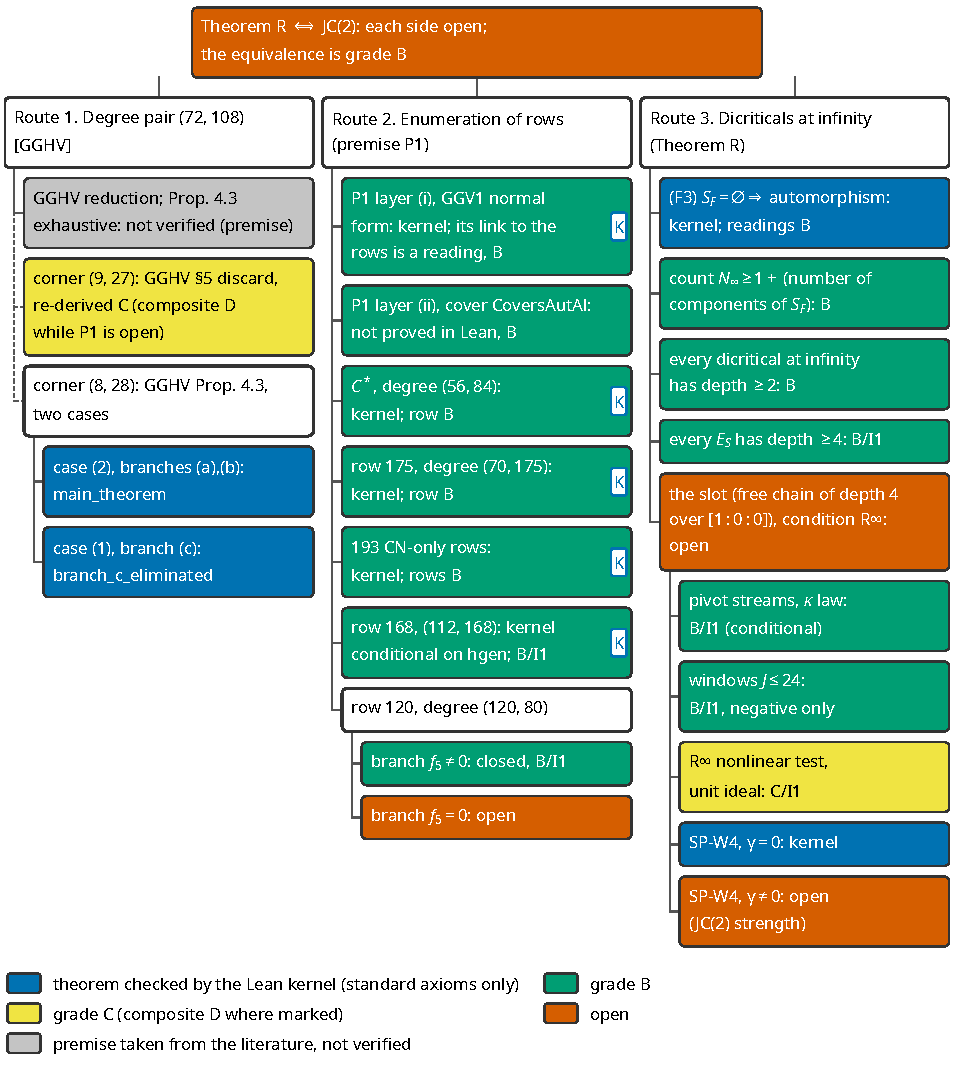
\includegraphics[width=\linewidth]{figures_jac/figJ2_status_map.pdf}
\caption{None of the three routes to Theorem~R is closed: each ends in an open box or in an unverified premise. Each box is one result or obligation, and its fill is its grade in the project's verification log. Blue is a theorem checked by the Lean kernel on the standard axioms, green is grade B, yellow is C, vermillion is open, and grey is a premise taken from the literature and not verified; white boxes only group results. A K badge on a green box means that the formal statement is a kernel theorem, while the row or step it is read as stays at grade B, because the passage from the printed row to the formal statement is a reading and because the enumeration premise P1 is grade B. Each box also states its grade in words, so the figure reads correctly in greyscale. Dashed edges mark the passage from a corner of $(72,108)$ to its normal form, which is GGHV's. The colours record grades; they are not a proof. The snapshot is the state at the close of the 25 November 2026 work (14:05 CST); compare Table~\ref{rp:tab:status}. The $\kappa$-law box is conditional (Figure~\ref{rp:fig:kappa}); the windows result is negative only and finite in range; (F3) is a formalization of a classical result.}
\label{rp:fig:status}
\end{figure}

The degree pair $(72,108)$ is eliminated only conditionally. Parts~I and~II eliminate the two cases of GGHV Proposition~4.3 in Lean, but the exclusion of $(72,108)$ rests on that proposition being correct and exhaustive (\cite{GGHV}, arXiv:2204.14178v1) and on the reduction chain, which is ledgered and not re-derived. The same holds for every row in this part: $C^*$, rows $168$, $175$ and the $193$ CN-only rows are eliminated in the kernel from their defining data, but their grade as eliminations of printed rows is B, because the enumeration premise is B and the R-def reading is B. Row~$120$ is half done. The layer-(i) normal-form theorem is a kernel theorem; the passage from it to the rows is a reading, and the covering statement of layer (ii) is an explicit Lean proposition that has not been proved.

The sharpest open problems are the following. First, layer~(ii) of the enumeration premise: regular-corner conditions on aligned first-edge data and a degree bound, which would make \texttt{CoversAutAl} a bounded decidable check. Second, SP-W4 at $\gamma\ne0$, which is of the strength of JC(2). Third, the condition R$\infty$ of the slot. Fourth, the build that would discharge hgen for row~$168$. Fifth, the branch $f_5=0$ of row~$120$, where consistency must be decided at layer $13$ or beyond. Sixth, the wiring of the formalized (F3) into the reduction step that uses it, with a check that the field degree is the same object on both sides. To these we add an audit of earlier verdicts that relied on msolve alone, and the case $m\ge4$, $\alpha_1=0$ of the Rodríguez Díaz reduction.

Figure~\ref{rp:fig:status} gathers these statuses into one map of the three routes; read each column from its heading down to the first vermillion or grey box, which is where that route stops.


\begin{center}
\refstepcounter{table}\label{rp:tab:status}%
\small
\begin{tabular}{@{}>{\raggedright\arraybackslash}p{5.6cm}>{\raggedright\arraybackslash}p{5.2cm}>{\raggedright\arraybackslash}p{3.2cm}@{}}
\toprule
Result & Form of evidence & Grade\\
\midrule
(P2) at a free point of $E_2$ (Part~III), November 11 & proof by hand; SymPy check & B, I1\\
$C^*$, degree $(56,84)$, from first edge and ratio & kernel (\texttt{cstar\_\allowbreak{}no\_\allowbreak{}pair\_\allowbreak{}firstEdge}) & 4K/I1; row B\\
$C^*$ certificate, 55 generators & kernel & 4K statement; chain B\\
Two encodings of $C^*$ agree & kernel (\texttt{span\_\allowbreak{}eq}) & 4K, I1\\
Gauge lemma G & kernel; reading & C$\to$4K; faithfulness B/I1\\
GGHV \S5 needs $\lambda\ne0$; solutions at $\lambda=0$ & three tools & B (gap, not counterexample)\\
$\lambda=0$ branch excluded & three tools; reduction in kernel & B, I2; overall B conditional\\
Lemma B, residue-free form & kernel (\texttt{lemmaB\_\allowbreak{}every\_\allowbreak{}rf}) & 4K/I1\\
Lemma S & kernel (\texttt{lemmaS}) & 4K/I1\\
Earlier ``Lemma B for all $m$'' is the weak form & reading, two-tool witness & B, I1 (correction E171)\\
Orevkov \S4.2 system, all parameters & kernel (\texttt{orev42\_\allowbreak{}all}) & 4K/I1 as transcribed\\
Transcription faithful to Orevkov 2001 & reading & B/I1\\
vdE 10.2.4 corrected; printed (i) refuted & kernel & 4K/I1; reading B\\
vdE 10.2.8, 10.2.13, 10.2.15, 10.2.18, 10.2.21 & kernel & 4K/I1\\
GGV1 normal form (``primera'') & kernel (\texttt{primera\_\allowbreak{}ekua4}) & 4K/I1; enumeration premise B\\
Row 175 & kernel; replay 1225/1225 & B\\
Row 168 & kernel, conditional on hgen & B/I1\\
Row 120, $f_5\ne0$ / $f_5=0$ & certificates & B/I1 / open\\
CNAt, T26At & kernel (\texttt{cnat}, \texttt{t26at}) & 4K/I1\\
193 CN-only rows & kernel & rows B\\
Cover interface & kernel (\texttt{jc2\_\allowbreak{}of\_\allowbreak{}coverCN}) & 4K/I1; layer (ii) B\\
SP-W4 at $\gamma=0$ / $\gamma\ne0$ & kernel / none & 4K/I1 / open\\
(F3) over any field of char.~0 & kernel (\texttt{F3\_\allowbreak{}field\_\allowbreak{}iff}) & 4K/I1; readings B\\
Slot: pivot forms, all $m\ge13$, run-A slice & hand lemmas, two tools & B/I1\\
Slot: window termination, $J\le24$ & Singular, msolve & B/I1, negative only\\
Slot R$\infty$ & none & open\\
Rodríguez Díaz Thm 3.12 step & two tools & B/I1 (gap)\\
GGV2 corollary false for Laurent pairs & two tools & B/I1\\
Theorem R (equivalently JC(2)) & none & open\\
\bottomrule
\end{tabular}

\smallskip
Table~\thetable. Main results of November 22--25, 2026, with the (P2) settlement of November 11, and the grades assigned in the verification log. ``Kernel'' means accepted by the Lean kernel with only the three standard axioms.
\end{center}

The work of this period strengthened the instruments without changing the verdict. Its most useful product may be negative in the best sense: a list of residual statements, each now precise enough that a proof or a counterexample would be recognized as such.
\appendix
\renewcommand{\thesection}{\Alph{section}}
\renewcommand{\theHsection}{app.\Alph{section}}
\section{Methods: software, verification and grades}\label{app:methods}

This appendix describes how the results of the paper were obtained and checked. It is written for a reader who wants to know exactly what kind of evidence stands behind each statement, and in particular how much of it rests on a proof checker, how much on computer algebra, and how much on reading a printed source.

\subsection{Software and hardware}

The formal proofs are written in Lean~4, version 4.34.0 (core commit \texttt{293d5d0}), with Lake 5.0.0 and the Mathlib library pinned at commit \texttt{5ed29652}. Exact symbolic computation used Singular 4.4.1 (and 4.3.1 on the remote machine; Part~I records some early runs under 4.3.2), SymPy 1.14.0 under Python 3.11, the Wolfram Engine 15.0 with WolframScript 1.14.0 (the Wolfram Language of Mathematica), python-flint 0.9.0 for fast arithmetic over $\mathbb{Q}$ and over prime fields, and msolve 0.9.5 for Gr\"obner bases and real solving. With msolve 0.9.5 we found that unexpanded input could be parsed incorrectly when parentheses were present, so every system sent to it was first expanded to a sum of monomials. Most heavy computations ran on a Google Cloud virtual machine with 24 virtual CPUs and 96\,GB of memory (machine type \texttt{n2-custom-24-98304}, zone \texttt{us-central1-a}); smaller checks ran locally. This document was typeset with Xe\LaTeX{} from TeX Live 2026. Every script, log and Lean file cited in the paper is in the repository named on the title page, or in the campaign archive described in Part~IV.

\subsection{What a kernel check certifies}

Lean reduces every proof to a term in a small type theory, and a short program, the \emph{kernel}, checks that term. When we say a statement is \emph{kernel-checked} we mean three things. The statement compiles as a Lean theorem with no \texttt{sorry}. The command \texttt{\#print axioms} applied to it lists only \texttt{propext}, \texttt{Classical.choice} and \texttt{Quot.sound}, the three axioms of Lean's standard foundations. And the formal statement has been read against the mathematical statement it is meant to express, with every hypothesis, quantifier and definition compared. The third step is a human reading and can fail; where a formal statement has not yet been compared line by line with a printed source we say so. A kernel check is therefore much stronger than a computer-algebra verdict, but it certifies the formal statement, not automatically the informal reading of it. Statements that were only read and compared, without a kernel proof, are called \emph{statement-audited}; that is a weaker category and we keep the two apart throughout. In particular, a Lean development that has been read in full and found free of \texttt{sorry} but whose kernel compilation has not been reproduced is not counted as kernel-checked.

\subsection{Cross-checks and planted controls}

A computer-algebra verdict that carries weight in an argument (an ideal containing $1$, a rank, a determinant, a Gr\"obner basis) is recomputed with a second program, typically Singular and SymPy, or Singular and FLINT, or the Wolfram Engine. Agreement of two programs written by different people guards against bugs in either, though not against a mistake in the shared formulation of the problem; for that, the formulation itself is re-derived from the source where possible.

A verification that never rejects anything is not evidence. We therefore use \emph{planted controls}: a deliberately false statement, or a deliberately corrupted input (a reversed inequality, a wrong coefficient, a \texttt{sorry} hidden in a Lean file), is mixed into the material handed to a check, without marking it. A check counts only if it rejects every plant. The record of each investigation in Part~IV lists the plants used and whether they were caught. The validation of this edition used the same device (Appendix~\ref{app:history}).

\subsection{Grades}

Every claim carries a grade under the author's evidence-accounting scheme (HLRE, version 5.1). A claim is graded, never a person or a program, and the grade attaches to the narrow statement printed, not to anything it might suggest. The letter grades mean the following. Grade~A is the strongest: for a deductive claim it means the statement is machine-checked or independently re-derived with every premise accounted for. Grade~B means strong, constrained support: for instance a complete exact computation cross-checked by two programs, or a careful proof that has not been machine-checked, or a kernel proof whose link to the intended mathematical statement passes through a reading that has not itself been formalized. Grade~C means a plausible claim with constrained but incomplete support, such as a proof sketch or a computation at a single degree. Grade~D means exploratory.

A second index records independence. I0 means the check used the same data that produced the claim; I1 means a new analysis by the same route, sharing choices with the original; I2 means an independent re-derivation by a check that did not see the original work, or a held-out test under a protocol fixed in advance; I3 means an independent team, dataset or instrument; I4 means independent replication together with a comparison against competing explanations. Kernel-checked results are written 4K in the record, so ``4K/I1'' means a kernel proof produced and checked within one line of work. For claims inside a formal system the record sometimes uses the finer labels F1 (machine-checked, or re-derived with a closed premise ledger), F2 (one independent route) and F3 (a single computational route).

A grade never rises by itself. When a result depends on a premise of lower grade, the result inherits the lower grade, and we say which premise is responsible. This is why, for example, several kernel theorems in Part~IV appear next to rows of the enumeration that remain at grade~B: the theorem is certain, but its application to the row passes through a step that is not.


\section{Revision history and corrections}\label{app:history}

Parts~I--III were drafted between September 28 and October 1, 2026, combined into one document on October 22, and revised on November 4 and November 22, 2026. Part~IV is new in the present edition. We record here what changed in this edition and which errors in the earlier ones it corrects, so that a reader who has the November 22 version can tell exactly what is different. Every correction listed below was first logged in the author's errata file (version 17, November 25, 2026, where items are numbered E1, E2, and so on), or in the audit of the journal galley proof of Part~II (November 13, 2026). We keep those numbers here so that each change can be traced to its source.

\paragraph{Corrections in Part~I.} The earlier text said that the corner $(9,27)$ is discarded in \S5 of \cite{GGHV}. The discard is in fact spread over Proposition~4.1, Corollary~5.7 and Theorem~5.1 there, and the reference now says so (E40). No other erratum concerns Part~I. The mathematics is unchanged. The exposition was rewritten from the beginning: a section on setting and notation now defines each object before it is used, the layer reduction is derived from an explicit bracket identity for layer terms, and the descent through the layers is written out step by step. Every algebraic step added in the rewrite was checked by a SymPy script (77 checks, all passing).

\paragraph{Corrections in Part~II.} A paragraph on the formalization of the degree-$19$ rigidity step was stale. It described the step as not yet formalized, although it had been proved in Lean, by \texttt{degree19\_\allowbreak{}rigidity} and the edge lemmas that \texttt{main\_\allowbreak{}theorem\_\allowbreak{}c\_\allowbreak{}of\_\allowbreak{}claim} calls directly, with no external certificate. The paragraph has been replaced (E36, with E152 and E156). The replacement says explicitly that the application to the degree pair $(72,108)$ remains conditional on GGHV Proposition~4.3. The galley audit found that one entry of the grade table was out of date: the emptiness of the chart had been proved in Lean on November 4, 2026 (\texttt{challenge\_\allowbreak{}target}), so its grade is A, not B. The rank argument of the whole-chart section is kept as an independent check at grade~B. A sentence about a Lean proof of the stratum $b_{11,20}\ne0$, left over from an earlier list, has been deleted. The file counts of the Lean development are now stated with their scopes: the full overlay builds $790$ modules, the branch-(c) directory has $686$ files, and the reflection descent consists of $504$ generated modules, which together with its main file make $505$, and with the bridge file the $506$ files of that directory. The earlier description of $505$ files as all generated is corrected to this. The corner $(9,27)$ citation is corrected as in Part~I (E40), and a gap in the printed treatment of $(9,27)$, an auxiliary constant used without a proof that it is nonzero, is now mentioned together with its separate exclusion (E80). Two smaller slips were fixed: a stray parenthesis, and theorem names typeset as file names (E44). Two listings that had been labelled as exact statements were abridged; they are now labelled as excerpts, and the definition of $\mathrm{NewtonNFc}$ is printed as it appears in the source. The two validation notes that preceded the table of contents in the November~22 edition have been worked into the body of Part~II.

\paragraph{Corrections in Part~III.} Lemma~\ref{td:lem:binary} was false as stated: it needs the hypothesis $g\ne0$, and $f=x$, $g=0$ is a counterexample. The hypothesis is added, and its applications already have $g\ne0$ (E1). The bibliography entry for arXiv:0801.4138, a withdrawn preprint that was listed but never cited, has been removed (E2). The counting proposition now states the hypothesis $c\notin G(D)$ that its proof uses, and the consequences drawn from it name their premises (E4, E5). Lemma~\ref{td:lem:linf} is in substance due to Borisov \cite{Borisov2009,Borisov2011}, and the first-blow-up lemma overlaps his results; both are now credited, and no novelty is claimed for them (E7, E13). An attribution paragraph after Proposition~\ref{td:prop:equiv} records that the forward direction of the equivalence with JC(2), the reduction to the birational case and the description of the non-properness set by dicritical series are classical \cite{Borisov2011,Keller1939,Borisov2009,Chau2007}; what is ours is the formulation in terms of the pencil (E20, E110). The open item on the binary-form step notes that this step has been formalized for $g\ne0$ outside the repository (E45). The proof of the bridge theorem has been rewritten to match its Lean formalization: the equations split by weight, so no descending induction is needed, and at weight $2$ the printed argument applied a rank lemma outside its hypotheses. The corrected proof uses two distinct centres at that weight, as the Lean proof does, and the rank lemma is restated for a single centre. No grade changes. Premise (P2) of the bridge theorem, listed as open (obligation O2) in the earlier editions, was settled for Keller maps on November 11, 2026; the proof is now Proposition~\ref{td:prop:P2} (grade B, I1), and the geometric reading of the bridge theorem needs (P1) alone. The section disclosing computational assistance has been removed from Part~III; its content is in Appendix~\ref{app:methods} and in the note at the end.

\paragraph{New material.} Part~IV reports investigations made in November 2026 on the obligations of Part~III. Each result there carries the grade recorded for it at the time of writing, and \S\ref{rp:sec:status} lists what is not established. Where a result of Part~IV bears on a statement of Parts~I--III, the earlier statement has been left as it was, with its original grade, and Part~IV says how it has moved.

\paragraph{Validation of this edition.} Before this edition was assembled, every changed or new claim was checked against the research record and every new citation against the source it cites. A deliberately false claim was planted among the claims to be checked, and the check rejected it. The details are in the file \filename{VALIDATION.md} distributed with the source.

\begin{thebibliography}{99}

\bibitem{GGHV} J.~A.~Guccione, J.~J.~Guccione, R.~Horruitiner, C.~Valqui, \textit{Increasing the degree of a possible counterexample to the Jacobian conjecture from 100 to 108}, arXiv:2204.14178v1 (2022).

\bibitem{Stothers} W.~W.~Stothers, \textit{Polynomial identities and Hauptmoduln}, Quart.\ J.\ Math.\ Oxford Ser.\ (2) \textbf{32} (1981), 349--370.

\bibitem{Davenport} H.~Davenport, \textit{On $f^3(t)-g^2(t)$}, Det Kongelige Norske Videnskabers Selskabs Forhandlinger \textbf{38} (1965), 86--87.

\bibitem{Moh} T.~T.~Moh, \textit{On the Jacobian conjecture and the configurations of roots}, J.\ Reine Angew.\ Math.\ \textbf{340} (1983), 140--212.

\bibitem{Santibanez} F.~Santiba\~nez-Leal, \textit{CAOS records EXP-061 and EXP-065}, GitHub repository \href{https://github.com/fsantibanezleal/CAOS_RESEARCH}{\filename{github.com/fsantibanezleal/CAOS\_RESEARCH}} (2026).

\bibitem{SantibanezPaper} F.~Santiba\~nez-Leal, \textit{CAOS v0.34}, Zenodo \href{https://doi.org/10.5281/zenodo.22834215}{doi:10.5281/zenodo.22834215} (2026).

\bibitem{JC125note} B.~D.~McCrary et al., \textit{The $(72,108)$ candidate for the planar Jacobian conjecture: a containment note}, Zenodo \href{https://doi.org/10.5281/zenodo.22941057}{doi:10.5281/zenodo.22941057} (2026).

\bibitem{ClaudeBlind} \textit{Independent blind replication: GGHV Proposition~4.3, normal form~(2)}, folder of the repository named on the title page (see the Note on assistance at the end of the paper), \href{https://github.com/brandonmccraryresearch-cloud/2D-Jacobian-Conjecture-Workspace/tree/main/tier1_blind_gghv43_nf2}{\textcolor{magenta}{\filename{tier1\_blind\_gghv43\_nf2/}}} in B.~D.~McCrary, \textit{2D-Jacobian-Conjecture-Workspace}, GitHub (2026), commit \texttt{37c73b67} (2026-09-25).

\bibitem{BranchABv19} B.~D.~McCrary, \textit{Elimination of the GGHV branch-(a,b) normal form at degree pair $(72,108)$: a certified computational audit. Layer reduction, top-layer classification, and final obstruction}, Zenodo \href{https://doi.org/10.5281/zenodo.23023490}{doi:10.5281/zenodo.23023490} (2026).

\bibitem{Helali} H.~Helali, \textit{Exact computer-assisted exclusion of the $(72,108)$ frontier in the two-dimensional Jacobian problem}, Zenodo \href{https://doi.org/10.5281/zenodo.21479814}{doi:10.5281/zenodo.21479814} (2026).

\bibitem{wstrinz} wstrinz, \textit{Structural analysis of the plane Jacobian $(72,108)$ candidate}, GitHub repository \href{https://github.com/wstrinz/plane-jacobian-72-108}{\filename{github.com/wstrinz/plane-jacobian-72-108}} (2026).

\bibitem{Jelonek1993} Jelonek, Z. \textit{The set of points at which a polynomial map is not proper.} Ann.\ Polon.\ Math.\ 58 (1993), no.~3, 259--266. doi:10.4064/ap-58-3-259-266.

\bibitem{Chau2009} Nguyen Van Chau. \textit{Pencil of irreducible rational curves and plane Jacobian conjecture.} arXiv:0905.3939.

\bibitem{AH2015} Abhyankar, S.~S., Heinzer, W.~J. \textit{Existence of dicritical divisors revisited.} arXiv:1508.06015.

\bibitem{AbhyankarSurvey} \textit{Abhyankar's work on dicritical divisors.} arXiv:1707.06733. A survey; it states no equivalence between dicriticals and the conjecture.

\bibitem{BBR1962} Bia\l{}ynicki-Birula, A., Rosenlicht, M. \textit{Injective morphisms of real algebraic varieties.} Proc.\ Amer.\ Math.\ Soc.\ 13 (1962), 200--203.

\bibitem{Restatement} McCrary, B.~D. \textit{The two-dicritical theorem, restated.} Unpublished working note, \filename{dicriticals-at-infinity/RESTATEMENT.md}, October 13, 2026. Not published or deposited.

\bibitem{Borisov2009} A.~Borisov, \textit{A geometric approach to the two-dimensional Jacobian conjecture}, arXiv:0912.4803v1 (2009).

\bibitem{Borisov2011} A.~Borisov, \textit{On resolution of compactifications of unramified planar self-maps}, arXiv:1110.5118 (2011; v4, 2012).

\bibitem{Borisov2015author} A.~Borisov, \textit{On the Stein factorization of resolutions of Jacobian self-maps of $\mathbb{P}^2$}, author's version of the paper in Beitr.\ Algebra Geom.\ \textbf{56} (2015), 299--312. The printed version has not been consulted.

\bibitem{Chau2007} Nguyen Van Chau, \textit{A note on singularity and non-proper value set of polynomial maps of $\mathbb{C}^2$}, arXiv:0710.5212 (2007).

\bibitem{Formanek1987} E.~Formanek, \textit{Two notes on the Jacobian conjecture}, Arch.\ Math.\ \textbf{49} (1987), 286--291.

\bibitem{GGV1} J.~A.~Guccione, J.~J.~Guccione, C.~Valqui, \textit{On the shape of possible counterexamples to the Jacobian conjecture}, J.\ Algebra \textbf{471} (2017), 13--74; arXiv:1401.1784v3.

\bibitem{GGV2} J.~A.~Guccione, J.~J.~Guccione, C.~Valqui, \textit{The two-dimensional Jacobian conjecture and the lower side of the Newton polygon}, arXiv:1605.09430v2 (2017).

\bibitem{Keller1939} O.-H.~Keller, \textit{Ganze Cremona-Transformationen}, Monatsh.\ Math.\ Phys.\ \textbf{47} (1939), 299--306, doi:10.1007/BF01695502. Cited for the birational case, from the 1939 reviews (Zbl 0021.15303, JFM 65.0713.02).

\bibitem{Orevkov2001} S.~Yu.~Orevkov, \textit{Counterexamples to the ``Jacobian conjecture at infinity''}, Proc.\ Steklov Inst.\ Math.\ \textbf{235} (2001), 173--201.

\bibitem{RD2024} L.~O.~Rodr\'iguez D\'iaz, \textit{On the integrality of \'etale extensions of polynomial rings}, arXiv:2403.02219v2 (2024).

\bibitem{vdE2000} A.~van den Essen, \textit{Polynomial Automorphisms and the Jacobian Conjecture}, Progress in Mathematics \textbf{190}, Birkh\"auser, Basel, 2000.

\bibitem{Wright1997} D.~Wright, \textit{Affine surfaces fibered by affine lines over the projective line}, Illinois J.\ Math.\ \textbf{41} (1997), no.~4, 589--605, doi:10.1215/ijm/1256068982.

\end{thebibliography}


\section*{Note on assistance}\addcontentsline{toc}{section}{Note on assistance}

The research reported here was carried out with agentic AI assistance, used for deep literature research and for writing Wolfram Language (Mathematica), Singular, Lean and SymPy code. This assistance cut the research time by roughly a thousandfold, from what would have been several years to a few months. Some of the cited records were produced in this way: the blind replication \cite{ClaudeBlind} and some independent re-derivations were made by separate AI systems, and the deposit \cite{JC125note} names the assistant as a co-author. Every result in the paper has been checked by the tools and procedures described in Appendix~\ref{app:methods}, and the author takes responsibility for all of it.

\end{document}
